%%%*******************************************************************************
%  Classe Latex SENAI CIMATEC, Version 0.0.0 16/04/2009
%
%  Define as normas e estilo das disserta��es e teses do SENAI CIMATEC
%
%  Author : Hernane Pereira
%%%-------------------------------------------------------------------------------

%%%-------------------------------------------------------------------------------
% Changes log
%%%-------------------------------------------------------------------------------
% Version 1.1.1 - 08/03/2005
% - Added support for amsmath, amsthm, amsfonts and amssymb as default
%
% Version 1.1.0 - 22/07/2004
% - updated university front page format
%
% Version 1.1.0 - 20/06/2003
% - Initial version
%%%-------------------------------------------------------------------------------

%%%-------------------------------------------------------------------------------
%  DOCUMENTATION WITH EXAMPLE
%%%*******************************************************************************

%%%-------------------------------------------------------------------------------
%%% Thesis default options
%%%-------------------------------------------------------------------------------
%\documentclass[subook]{Classes/PPGMCTI}
%\documentclass[sureport]{Classes/PPGMCTI}

%%%-------------------------------------------------------------------------------
%%% Thesis custom options
%%%-------------------------------------------------------------------------------

%%% Fancy page headings
%\documentclass[fancyheadings, subook]{Classes/PPGMCTI}
%\documentclass[fancyheadings, sureport]{Classes/PPGMCTI}

%%% Fancy chapters and sections headings
%\documentclass[fancychapter, subook]{Classes/PPGMCTI}
%\documentclass[fancychapter, sureport]{Classes/PPGMCTI}

%%% Fancy page , chapters and sections headings
%\documentclass[fancyheadings, fancychapter, subook]{Classes/PPGMCTI}
%\documentclass[fancyheadings, fancychapter, sureport]{Classes/PPGMCTI}
\documentclass[fancyheadings, fancychapter, sureport]{PPGMCTI}

%%%-------------------------------------------------------------------------------
%%% Thesis Commands (ONLY with fancy page headings)
%%%-------------------------------------------------------------------------------

%%%Page header line width
%\footlinewidth{value}

%%%Page footer line width
%\headlinewidth{value}

%%%Page header and footer line width
%\headingslinewidth{value}

%%%Page header and footer lines without text
%\headingslinesonly

%%%The default line width is 0.3pt.
%%%Set the value to 0pt to remove the page header and/or footer line

%%%-------------------------------------------------------------------------------
%%% SUThesis Supported Graphic Formats
%%%-------------------------------------------------------------------------------
% The figures formats supported depend upon the selected output file
% Include your figure without the extention, the SUThesis will automatically
% search the predefined `Figures' directory tree for the right file format.
%
% - The pdfLaTEX (PDF) supports graphics inclusions in PDF, JPG, PNG, and
%   MetaPost (with .mps extention) formats.
%
% - The Latex (DVI) supports graphics inclusions in EPS and PS formats.
%%%-------------------------------------------------------------------------------


%%%-------------------------------------------------------------------------------
%%% �rvore de diret�rio PPGMCTI
%%%-------------------------------------------------------------------------------
%  Diret�rio
%       \Classes        (requerido)
%       \Figures        (requerido) --------------------------------->
%       \Figures\PDF    (optional)
%       \Figures\JPG    (optional) Figures located within these
%       \Figures\PNG    (optional) folders are searched automatically
%       \Figures\MPS    (optional)  by the PPGMCTI class.
%       \Figures\EPS    (optional)
%       \Figures\PS     (optional) <--------------------------------
%       \Tables         (requerido)
%       \Others         (requerido)
%       \Chapters       (requerido)
%       \Appendices     (optional)
%       \References     (requerido)
%%%-------------------------------------------------------------------------------

%%%-------------------------------------------------------------------------------
%%% PDF File Summary
%%%-------------------------------------------------------------------------------
\ifpdf
    \hypersetup{ % backref,
                colorlinks  = true,
                pdftitle    = Sistema Generativo de Projeto Aplicado ao Desenho e Otimiza��o da Estrutura de um Shed,                pdfauthor   = {Fernando Ferraz Ribeiro,ffribeiro@gmail.com},
                pdfsubject  = Mestre em MCTI,
                pdfcreator  = Subtitulo,
                pdfproducer = PDFLatex,
                pdfkeywords = {Sistemas de Projeto Generativo, Grafost�tica, Geometria, Arquitetura ,Otimiza��o}
    }
 \fi

%%%-------------------------------------------------------------------------------
%%% Required packages
%%%-------------------------------------------------------------------------------
% - ifthen
% - setspace
% - amsmath
% - amsfonts
% - amssymb
% - amsthm
% - eucal
% - graphics
% - fancyhdr
%%%-------------------------------------------------------------------------------

%%%-------------------------------------------------------------------------------
%%% Optional packages
%%%-------------------------------------------------------------------------------
\usepackage[latin1]{inputenc}
\usepackage{longtable}
\usepackage{multirow}
\usepackage{lscape}
\usepackage{graphicx}
\usepackage{wrapfig}
\usepackage{float,subfigure}
%\usepackage{cite}
\usepackage[left=3cm,top=3cm,right=2cm,bottom=2cm]{geometry}
%\usepackage[alf,abnt-etal-list=1]{abntex2cite} 
%\usepackage[alf,abnt-etal-list=5]{abntcite}
\usepackage{algorithm}
\usepackage{algorithmic}
\usepackage{ifpdf}

\usepackage[procnames]{listings}
\usepackage{listingsutf8}
\usepackage{color}

\usepackage[alf]{abntex2cite} 
%\usepackage[style=authoryear-comp,
%     hyperref,
%     backend=biber,
%     isbn=false,
%     doi=false,
%     url=false,     
%     date=year]{biblatex}

%\addbibresource{References/library.bib}
%Tables and Figures Caption
\setlength{\LTcapwidth}{\textwidth}

%\newtheorem{theorem}{Teorema}
%\newtheorem{definition}[theorem]{Defini\c{c}\~ao}


%%%-------------------------------------------------------------------------------
%%% Start thesis root document
%%%-------------------------------------------------------------------------------
\begin{document}




    %%----------------------------------------------------------------------------
    %% Define the title page
    %%----------------------------------------------------------------------------
    \university{SENAI CIMATEC}
%    \faculty{Pro\-gra\-ma de P\'os-gra\-dua\-\c{c}\~ao em Mo\-de\-la\-gem Com\-pu\-ta\-cio\-nal e Tec\-no\-lo\-gia In\-dus\-trial}
    \faculty{Pro\-gra\-ma de P�s-gra\-dua\-��o em Mo\-de\-la\-gem Com\-pu\-ta\-cio\-nal e Tec\-no\-lo\-gia In\-dus\-trial}
%    \school{School of Mathematics}
    \course{Mestrado em Modelagem Computacional e Tecnologia Industrial}
    \typework{Disserta\c{c}\~ao de mestrado}
%    \typework{Tese de doutorado}
%    \course{Doutorado em Modelagem Computacional e Tecnologia Industrial}
    \thesistitle{Sistema Generativo de Projeto Aplicado ao Desenho e Otimiza��o da Estrutura de um \textit{Shed}}
    \hidevolume
    \thesisvolume{Volume 1 of 1}
    \thesisauthor{Fernando Ferraz Ribeiro}
    \thesisadvisor{Davidson Martins Moreira}
%   \hidecoadvisor
    \thesiscoadvisor{Arivaldo Le�o de Amorim}
    \thesisdegreetitle{Mestre em Modelagem Computacional e Tecnologia Industrial}
%    \thesisdegreetitle{Doutor em Modelagem Computacional e Tecnologia Industrial}
%    \thesismonthyear{M\^es de Ano}
    \thesismonthyear{Abril de 2015}

    \maketitlepage

    %%----------------------------------------------------------------------------
    %% Inserir Folha de rosto, Nota de estilo, folha de assinaturas, dedicatoria
    %%----------------------------------------------------------------------------
    % !TeX encoding = ISO-8859-1
% !TeX spellcheck = pt_BR
%==========================================================
%        Document: PPGMCTI
%        File....: FolhaRosto.TEX
%        Author..: Hernane Pereira
%        Date....: 16 de abril de 2009
%==========================================================
\begin{folharosto}

\begin{center}
\theauthor
\end{center}
\ \\
\ \\
\ \\
\ \\
\ \\
\begin{spacing}{2}
   \begin{center}
   {\LARGE {\bf \thetitle}}
   \end{center}
\end{spacing}
\ \\
\ \\
\ \\
\begin{flushright}

   \begin{list}{}{
      \setlength{\leftmargin}{4.5cm}
      \setlength{\rightmargin}{0cm}
      \setlength{\labelwidth}{0pt}
      \setlength{\labelsep}{\leftmargin}}

      \item \thetypework apresentada ao \thefaculty, Curso de \thecourse
      do \theuniversity, como requisito parcial para a obten\c{c}\~ao do
      t\'itulo de {\bf \thedegreetitle}.

      \begin{list}{}{
      \setlength{\leftmargin}{0cm}
      \setlength{\rightmargin}{0cm}
      \setlength{\labelwidth}{0pt}
      \setlength{\labelsep}{\leftmargin}}

      \item \'Area de conhecimento: Interdisciplinar

      \item Orientador: \theadvisor
      \newline \hspace*{2.1cm}  {\it \theuniversity}

      % Caso haja um co-orientador(a), retirar os '%' das duas linhas seguintes 
      \item Co-orientador: \thecoadvisor
      \newline \hspace*{2.1cm}  {Faculdade de Arquitetura - UFBA} % ou inserir o nome da IES do(a) Co-orientador(a) no caso da IES ser diferente do SENAI CIMATEC

      \end{list}
   \end{list}

\end{flushright}
\ \\
\ \\
\ \\
\ \\
%\begin{spacing}{1.5}
   \begin{center}
   Salvador \par
   \theuniversity \par
   2015
   \end{center}
%\end{spacing}

\end{folharosto}

    % !TeX encoding = ISO-8859-1
% !TeX spellcheck = pt_BR
%==========================================================
%        Document: PPGMCTI
%        File....: NotaEstilo.TEX
%        Author..: Hernane Pereira
%        Date....: 16 de abril de 2009
%==========================================================

\begin{notaestilo}
Esta \thetypeworkthree foi elaborada considerando as normas de
estilo (i.e. est\'eticas e estruturais) propostas aprovadas pelo
colegiado do \thefacultytwo e est\~ao dispon\'iveis em formato
eletr\^onico ({\it download} na P\'agina Web
http:$//$ead.fieb.org.br$/$portal\_faculdades$/$dissertacoes-e-teses-mcti.html
ou solicita\c{c}\~ao via e-mail \`a secretaria do
programa) e em formato impresso somente para consulta. \\

Ressalta-se que o formato proposto considera diversos itens das
normas da Associa\c{c}\~ao Brasileira de Normas T\'ecnicas (ABNT),
entretanto opta-se, em alguns aspectos, seguir um estilo pr\'oprio
elaborado e amadurecido pelos professores do programa de
p\'os-gradua\c{c}\~ao supracitado.

\end{notaestilo}

    % !TeX encoding = ISO-8859-1
% !TeX spellcheck = pt_BR
%==========================================================
%        Document: PPGMCTI
%        File....: FolhaAssinaturas.TEX
%        Author..: Hernane Pereira
%        Date....: 16 de abril de 2009
%==========================================================

\begin{folhaassinaturas}

%\thispagestyle{empty}

%*********************************************************************
% O codigo seguinte foi extraido do arquivo DissertacaoMIMC_Estilo.tex
%*********************************************************************

\def\signature#1#2{\parbox[b]{1in}{\smash{#1}\vskip12pt}
\hfill \parbox[t]{3in}{\shortstack{\vrule width 3in height
0.4pt\\\small#2}}}

\def\InstituicaoMembro#1#2{\parbox[b]{1in}{\smash{#1}\vskip12pt}
\hfill \parbox[t]{3in}{\shortstack{\vrule width 3in \\\small#2}}}

\def\signaturepage{%

    \begin{spacing}{1.5}
        \begin{center}
        {\LARGE \theuniversity} \\
        {\large \thefaculty} \\
        {\large \thecourse} \\
        \end{center}
    \end{spacing}

   \vskip 0.25in plus 0.4in minus 0.1in

    \begin{spacing}{1.5}
        \begin{sloppypar}
        A Banca Examinadora, constitu\'ida pelos professores abaixo
        listados, leram e recomendam a aprova\c{c}\~ao [com distin\c{c}\~ao] da
        \thetypeworktwo, intitulada ``\thetitle",
        apresentada no dia (dia) de (m\^es) de (ano), como requisito
        parcial para a obten\c{c}\~ao do t\'itulo de {\bf \thedegreetitle}.\\
        \end{sloppypar}
    \end{spacing}

    \def\sigskip{\vskip0.15in plus 0.2in minus 0.1in}
    \def\beginskip{\vskip0.3875in plus 0.2in minus 0.1in}

    \beginskip
    \signature{Orientador:}{Prof. Dr. \theadvisor} \\
    \InstituicaoMembro{}{\theuniversity} \\

    % Caso haja um co-orientador(a), retirar os '%' das quatro linhas seguintes 
    \sigskip
    \beginskip
    \signature{Co-orientador:}{Prof. Dr. \thecoadvisor} \\
    \InstituicaoMembro{}{Faculdade de Arquitetura - UFBA} \\ % ou inserir o nome da IES do(a) Co-orientador(a) no caso da IES ser diferente do SENAI CIMATEC
    
    \sigskip
    \beginskip
    \signature{Membro externo da Banca:}{Prof. Dr. Felipe Tavares da Silva} \\
    \InstituicaoMembro{}{Faculdade de Arquitetura - UFBA} \\


    \sigskip
    \beginskip
   	\signature{Membro interno da Banca:}{Prof. Dr. Renelson Ribeiro Sampaio} \\
   	\InstituicaoMembro{}{\theuniversity} \\
   	
   	\sigskip
   	    \beginskip
   	   	\signature{Membro interno da Banca:}{Prof. Dr. Gilney Figueira Zebende} \\
   	   	\InstituicaoMembro{}{\theuniversity} \\
   	

    \vfill
    \newpage
    \setcounter{page}{3}
}
%*********************************************************************


\signaturepage


\end{folhaassinaturas}

    % !TeX encoding = ISO-8859-1
% !TeX spellcheck = pt_BR

%==========================================================
%        Document: PPGMCTI
%        File....: Dedicatoria.TEX
%        Author..: Hernane Pereira
%        Date....: 16 de abril de 2009
%==========================================================

\begin{dedicatoria}
%\thispagestyle{empty}
\ \\
\ \\
\ \\
\ \\
\ \\
\ \\
\ \\
\ \\
\ \\
\ \\
\ \\
\ \\
\ \\
\ \\
\ \\
\ \\
\ \\
\ \\
\ \\
\ \\
\ \\
\ \\
\ \\
\ \\
\ \\
\ \\
\ \\
\ \\
\ \\



\begin{flushright}
Dedico este trabalho a minha m�e,\\  \textbf{Aidil Nunes Ferraz Ribeiro},\\ pelo amor e apoio que nunca me faltaram;\\ e a mem�ria de meu pai,\\ \textbf{Ubirajara Gomes Ribeiro},\\ pelas inesquec�veis li��es de Geometria, \\mas principalmente, \\pelos esquadros e compassos da vida.
\end{flushright}
\end{dedicatoria}

    % !TeX encoding = ISO-8859-1
% !TeX spellcheck = pt_BR
%==========================================================
%        Document: PPGMCTI
%        File....: Agradecimentos.TEX
%        Author..: Hernane Pereira
%        Date....: 16 de abril de 2009
%==========================================================

\begin{agradecimentos}

Um trabalho desta natureza n�o pode ser realizado sem a inestim�vel ajuda de muitas pessoas. � o resultado de experi�ncias profissionais, pessoais a acad�micas que se acumularam, ganharam forma e me fizeram olhar para minha trajet�ria profissional com felicidade e gratid�o. Agrade�o a meu orientador, Davidson Martins Moreira e meu co-orientador, Arivaldo Le�o de Amorim, por todos os conselhos, cr�ticas, orienta��es e pelo trato amistoso e paciente que sempre me reservaram. Aos professores do programa de p�s-gradua��o PPG-MCTI e aos professores e palestrantes convidados, tanto pelo conhecimento dividido, quanto pela oportunidade de crescimento acad�mico e pessoal que me proporcionaram. Aos funcion�rios do colegiado e secretaria do mesmo programa, pela maneira sol�cita que exercem suas fun��es. Aos colegas de turma, pelo ambiente de amizade e colabora��o que marcou nossa conviv�ncia. � equipe do LCAD da Faculdade de Arquitetura da UFBA, e a professora Natalie Johanna Groetelaars, que me receberam durante a atividade de tiroc�nio docente, tanto pela oportunidade de acompanhar as aulas e o desenvolvimento da turma durante os trabalhos e avalia��es, quanto pelos conhecimentos divididos e multiplicados. � equipe do Instituto Brasileiro de Tecnologia do Habitat, representada pelo seu presidente, o arquiteto Jo�o Filgueiras Lima (Lel�), pelo per�odo de intenso trabalho e pela vis�o do papel e da profiss�o de arquiteto que fui apresentado. � equipe do escrit�rio Eleve Engenharia, onde pude aprimorar meus conhecimentos sobre estruturas. Aos membros das bancas de qualifica��o e defesa, pelas cr�ticas e corre��es fundamentais. Aos amigos arquitetos, companheiros de muitos projetos e colabora��es: Deraldo Tourinho, Arlindo Esteve, Daniel Gomes, M�rcio Targa, M�rio Vitor Bastos e Luiz Villa. Aos amigos pesquisadores de diversas �reas, pelas conversas e conselhos: Sandra Maria Ferraz Mello (amiga, tia e madrinha), Alexis Dourado Guedes, Lorena Guedes, Marcos Rodrigues, Lia Seixas e Paolo Bruni. � fam�lia de meu tio, Archibaldo Ferraz Melo, com um pedido de desculpas por ter alterado o roteiro de suas f�rias para que me trouxessem de presente um livro utilizado nesta pesquisa. Ao grande amigo Alessandro Soares, a quem sempre recorro nas d�vidas com o idioma ingl�s e conselhos sobre muito mais. Aos amigos que n�o desistiram de mim, me procurando mesmo sabendo que eu passaria os fins de semana imerso em trabalho: Maur�cio Cerqueira, Rog�rio Ribeiro (amigo e irm�o), Norbert Siering, Carlos Pereira, Miguel Cordeiro e Juliano Pontes. � minha grande amiga Carolina de Britto Fernandes, pelo carinho e apoio em todas as horas. Agrade�o tamb�m a todos os amigos e familiares, que acreditando e me incentivando tornaram essa jornada poss�vel.






\ \\

\noindent
Salvador, Brasil \hfill \theauthor\\
30 de \mesdeano
\end{agradecimentos}


%%%-------------------------------------------------------------------------------
%%% Definicao de comandos para apresentar algoritmos em portugues
%%%-------------------------------------------------------------------------------
\definecolor{keywords}{RGB}{0,0,255}
\definecolor{comments}{RGB}{100,100,100}
\definecolor{red}{RGB}{160,0,0}
\definecolor{green}{RGB}{0,150,0}
\definecolor{gray}{RGB}{120,120,120}
 
\lstset{language=Python,
        numbers=left,                   
        numberstyle=\tiny\color{gray},  
        stepnumber=4,
        inputencoding=utf8/latin1, 
        basicstyle=\ttfamily\small, 
        keywordstyle=\color{keywords},
        commentstyle=\color{comments},
        stringstyle=\color{red},
        showstringspaces=false,
        identifierstyle=\color{green},
        showlines = false,
        breaklines = false,
        procnamekeys={def,class}}
 



\renewcommand{\listalgorithmname}{Lista de Algoritmos}

\renewcommand{\algorithmicrequire}{\textbf{requer:}}
\renewcommand{\algorithmicensure}{\textbf{garantir:}}
\renewcommand{\algorithmicend}{\textbf{fim}}
\renewcommand{\algorithmicif}{\textbf{se}}
\renewcommand{\algorithmicthen}{\textbf{ent�o}}
\renewcommand{\algorithmicelse}{\textbf{sen�o}}
\renewcommand{\algorithmicelsif}{\textbf{sen�o se}}
\renewcommand{\algorithmicendif}{\textbf{fim se}}
\renewcommand{\algorithmicfor}{\textbf{para}}
\renewcommand{\algorithmicforall}{\textbf{para todo}}
\renewcommand{\algorithmicdo}{\textbf{fa�a}}
\renewcommand{\algorithmicendfor}{\textbf{fim para}}
\renewcommand{\algorithmicwhile}{\textbf{enquanto}}
\renewcommand{\algorithmicendwhile}{\textbf{fim enquanto}}
\renewcommand{\algorithmicloop}{\textbf{loop}}
\renewcommand{\algorithmicrepeat}{\textbf{repetir}}
\renewcommand{\algorithmicuntil}{\textbf{at�}}
\renewcommand{\algorithmicto}{\textbf{at�}}
\renewcommand{\algorithmiccomment}[1]{\hskip$\rightarrow$ #1}
\floatname{algorithm}{Algoritmo}


    %%----------------------------------------------------------------------------
    %% Resumo/abstract, sum�rio e siglas
    %%----------------------------------------------------------------------------

    \begin{romanpagenumbers}
        % !TeX encoding = ISO-8859-1
% !TeX spellcheck = pt_BR

\begin{thesisresumo}
O presente trabalho � uma investiga��o sobre a teoria e as aplica��es dos sistemas generativos de projeto como ferramenta de aux�lio na tomada de decis�es para a concep��o de formas na ind�stria da constru��o civil. Adotando uma metodologia experimental, um conjunto de algoritmos foi proposto como instrumentos de concep��o e desenho de um grupo de treli�as de suporte de uma cobertura tipo \textit{shed}, inspiradas na obra do arquiteto Jo�o Filgueiras Lima (Lel�). Al�m da gera��o de formas, o sistema conta com uma ferramenta de an�lise de estruturas, cuja modelagem foi baseada na Grafost�tica. Uma metodologia de trabalho e abordagem das quest�es relativas ao projeto arquitet�nico � proposta, e as contribui��es deste m�todo para a concep��o de elementos construtivos s�o avaliadas e discutidas.




\end{thesisresumo}
\hfill \break

Palavas Chave: Sistemas Generativos de Projeto, Algoritmos Generativos, Modelagem Param�trica, Grafost�tica, Arquitetura.

        % !TeX spellcheck = en_US
% !TeX encoding = ISO-8859-1


\begin{thesisabastract}
This Dissertation is a research on the theory and applications of the generative design systems as a tool in decision making for defining forms in the construction industry. Adopting an experimental methodology, a set of algorithms was proposed as assisting instruments aimed to design a group of shed trusses inspired by the work of architect Jo�o Filgueiras Lima (Lel�). Besides the generation of forms, the system has a structural analysis tool, which was based on Graphical Statics. A working methodology and an approach to architectural design related topics is proposed, and the contributions of this method for the design of building elements are evaluated and discussed.


\end{thesisabastract}

\hfill \break
Keywords: Generative Design Systems, Generative Algorithms, Parametric Modeling, Graphical Statics, Architecture.
        % Make list of contents, tables and figures
        \thesiscontents
        %Include other required section
        \begin{thesisabbreviations}
\begin{footnotesize}
\begin{longtable}[l]{p{2cm}l}
  AC    \dotfill & Aut�matos Celulares\\
  AG    \dotfill & Algoritmos Generativos\\
  BIM   \dotfill & Building Information Modeling \\
  CG    \dotfill & Computa��o Gr�fica\\
  DOF   \dotfill & Design Optimization and Fabrication\\
  DV    \dotfill & Diagrama de Voronoi\\
  FG    \dotfill & Forma Geom�trica\\
  GF    \dotfill & Gram�ticas de Forma\\
  GS    \dotfill & Grafost�tica (Est�tica Gr�fica) \\
  ICC   \dotfill & Industria da Constru��o Civil \\
  LS    \dotfill & L-Systems\\
  MPR   \dotfill & Modelos de Par�metros e Restri��es\\
  PF    \dotfill & Pol�gono de For�as\\
  SA    \dotfill & Simulated Annealing\\
  SGP   \dotfill & Sistema Generativo de Projeto \\
  SI    \dotfill & Swarm Intelligence\\
  
  
  
  
  
  
\end{longtable}
\end{footnotesize}
\end{thesisabbreviations}


        %Switch the page numbering back to the default format
    \end{romanpagenumbers}

    %%----------------------------------------------------------------------------
    %% Include thesis chapters
    %%----------------------------------------------------------------------------
    \parskip=\baselineskip
    % !TeX encoding = ISO-8859-1
% !TeX spellcheck = pt_BR
\chapter{Introdu\c{c}\~ao}
\label{chapter:introducao}

\begin{flushright}
  "Existe geometria no som das cordas;\\
   existe m�sica no espa�amento das esferas"\\
  \ \\
  (Atribuido � Pit�goras de Samos)
\end{flushright}

No decorrer dos �ltimos 50 anos, grandes mudan�as tem acontecido na Ind�stria da Constru��o Civil (\textbf{ICC}). As atividades de planejar e transformar o espa�o ao redor de si, almejando uma ocupa��o ideal e deparando-se inevitavelmente com as poss�veis apropria��es reais, foram subitamente abordadas por novas formas, m�todos de trabalho, demandas, cr�ticas e paradigmas, est�ticos e t�cnicos. � interessante notar o qu�o pequeno � esse espa�o de tempo em uma atividade cuja origem se encontra ligada � das primeiras civiliza��es humanas. 

A for�a que as quest�es ecol�gicas gradativamente ganharam, desde a d�cada de 1960, levaram as atuais preocupa��es de conserva��o de energia na fabrica��o, execu��o e uso das edifica��es. A Computa��o Gr�fica (CG) desenvolve-se no mesmo per�odo e colocou a disposi��o dos projetistas, primeiro novas ferramentas de desenho que rapidamente substituem a prancheta como instrumento prevalente no mercado, para ent�o terem a sua rec�m conquistada hegemonia desafiada por sistemas param�tricos de projeto, algoritmos generativos (\textbf{AG}), Sistemas Generativos de Projeto (\textbf{SGP}) e pela aplica��o do conceito BIM (\textbf{\textit{Building Information Modeling}}). Algoritmos e programas de an�lise dos diversos comportamentos do edif�cio proporcionaram tanto uma maior velocidade de trabalho, quanto crit�rios de julgamento mais objetivos. A otimiza��o ganha import�ncia pelo valor que se tem dado ao desempenho energ�tico das constru��es e economia de recursos na execu��o.

A crise propositiva do Movimento Moderno da Arquitetura, que simbolicamente culmina na demoli��o do conjunto habitacional Pruitt-Igoe em 1972, pode ser encarada como o rebatimento da crise do modelo mecanicista do universo na Filosofia das Artes. No livro "Complexidade e Contradi��o na Arquitetura", um manifesto e um dos textos chave para o estudo est�tico deste per�odo de transi��o, Robert  \citeonline{venturi1977} transforma o preceito do design minimalista \textbf{\textit{"less is more"}}(menos � mais) do arquiteto Mies van der Rhoe em \textbf{\textit{"less is a bore"}}(menos � um t�dio), afirmado que uma "Simplicidade for�ada resulta em uma uma simplifica��o excessiva"\footnote{\textit{Forced simplicity results in oversimplification.}}. Se parte do modernismo tem sua inspira��o nas linhas aerodin�micas dos carros, trens e aeronaves \cite{lecorbusier2000}, Paolo \citeonline[p. 35]{portoghesi2002}, em outro texto fundamental da mesma �poca, aponta o fato de que "(...)calculadoras eletr�nicas n�o s�o m�quinas no sentido tradicional, de transforma��o de energia, mas instrumentos que operam de forma an�loga ao c�rebro humano", dentre os motivos da atual inadequa��o dos valores que nortearam grande parte da produ��o arquitet�nica da primeira metade do s�culo XX. 

 \citeonline{Oxman2006} reconhece o Museu Guggenheim de Bilbao como um catalizador da complexidade deste momento da Arquitetura em diversos contextos. Principalmente por introduzir, nas suas superf�cies met�licas, curvas detalhadas com o suporte do \textit{software} CATIA, a complexidade de novas formas geometricas, livres de formalimos anteriores\footnote{\textit{In architecture, the Guggenheim Museum, Bilbao by Frank Gehry was the most prominent catalyst of theorizing new formal directions and postulating new design methods. Beyond the Postmodern sensibility of complexity through "heterotopia", or complex hybrids, the Guggenheim introduced the complexity of new geometric approaches freed from a priori formalisms, such as linguistic formalisms.}}. \citeonline{picon2011} aponta a ret�cula das fachadas do \textit{Young Museum}(2005) dos arquitetos Herzog \& de Meuron como um convite para uma experi�ncia t�til, diluindo as barreiras entre objeto e observador, conceito que, segundo o autor, muitos dos projetistas que exploram as potencialidades das ferramentas de projeto digital se identificam. Peter Eisenman \cite[p. 130-135]{eisenman1996} prop�e na sua "Casa Guardiola" de 1988 um espa�o resultante de opera��es matem�ticas entre s�lidos sobrepostos (interse��o, subtra��o...) realizadas em projeto atrav�s de comandos de um programa CAD 3D. \citeonline[p. 64]{mitchell2008} identifica nas formas fluidas e din�micas de alguns projetos contempor�neos, citando os trabalhos da arquiteta iraniana Zaha Hadid, uma alus�o ao ambiente computacional que os originou. O grupo de arquitetos ingleses Archigram, reunidos por volta de 1961 em torno da revista de mesmo nome onde apresentavam sua "abordagem infraestrutural, leve e \textit{high-tech}"\cite{frampton2000} da Arquitetura. Na proposta intitulada \textit{Instant City} (1969), imaginava-se que "as unidades habit�veis estivessem ligadas(...) a uma megaestrutura informacional que alimentaria e possibilitaria a maleabilidade do cotidiano urbano" \cite[p. 104-105]{duarte1999arquitetura}. A plena realiza��o deste ideal est�tico s� aconteceu ap�s o desenvolvimento da tecnologia CAD, como no projeto do Museu de Arte de Graz (\textit{Kunsthaus Graz}, conecido tamb�m pelo apelido de \textit{Friendly Alien}), inaugurado em 2003, de autoria de um dos antigos membros do grupo, o arquiteto Peter Cook. Coincidindo com um per�odo importante na difus�o das estruturas de informa��o atualmente dispon�veis.

A presente pesquisa prop�e um m�todo de trabalho onde aspectos estruturais e est�ticos de uma determinada treli�a de sustenta��o de coberturas s�o analisados com o aux�lio de algoritmos generativos, uma ferramenta de an�lise estrutural cuja modelagem foi baseada em alguns m�todos da Grafost�tica e a possibilidade de  utiliza��o desta an�lise em um experimento de otimiza��o da forma. Visando a aplicabilidade na pr�tica projetual de alguns dos conceitos que vem mudando a maneira de encarar o projeto arquitet�nico, bem como a sempre presente necessidade de comunica��o e debate entre alguns dos profissionais envolvidos no processo. Um exerc�cio onde a complexidade inerente � Arquitetura, mostrada na mistura de t�cnica, tecnologia e est�tica que a define, pode ser apreciada e estudada enquanto procura-se colaborar com os debates em torno dos seus atuais paradigmas.  


\section{Defini\c{c}\~ao do Problema}
\label{section:definicaoproblema}
O experimento realizado utiliza um \textbf{Sistema Generativo de Projeto} pass�vel de ser utilizado por arquitetos como ferramenta de aux�lio nos primeiros est�gios de concep��o e defini��o de um elemento de projeto a ser desenvolvido, bem como servir de ponto de partida do di�logo com outras equipes, particularmente com os escrit�rios de c�lculo e detalhamento de estruturas. O conceito de projeto generativo pode ser definido de maneira simples como "(...)um algoritmo ou processo baseado em regras pelo qual v�rias potenciais solu��es de projeto podem ser criadas"\footnote{\textit{Generative Design can be broadly defined as an algorithmic or rule-based process through which various potential design solutions can be created.}}\cite{fasoulaki2008}.

O algoritmo em foco pode ser conceitualmente dividido em 3 partes que ser�o adiante explicadas:

\begin{itemize}
\item Um modelo geom�trico baseado em par�metros e restri��es;
\item Um algoritmo de an�lise estrutural;
\item Um m�todo de otimiza��o.
\end{itemize}

Toda atividade de projeto, em qualquer �rea, mas particularmente nas que tem por objetivo a confec��o de um produto espec�fico, agrega em si uma complexidade de t�picos e �reas do conhecimento. No caso da constru��o, principalmente vista pelo prisma da Arquitetura, onde t�cnica, humanidades e arte se mesclam de forma peculiar, o entrela�amento de diversos campos do saber apresenta um contorno n�o menos complexo. O modelo te�rico representado na Figura \ref{figura:mod} procura ilustrar as rela��es centrais confrontadas e aliadas neste trabalho.
 
\begin{figure}[!ht]
\begin{center}
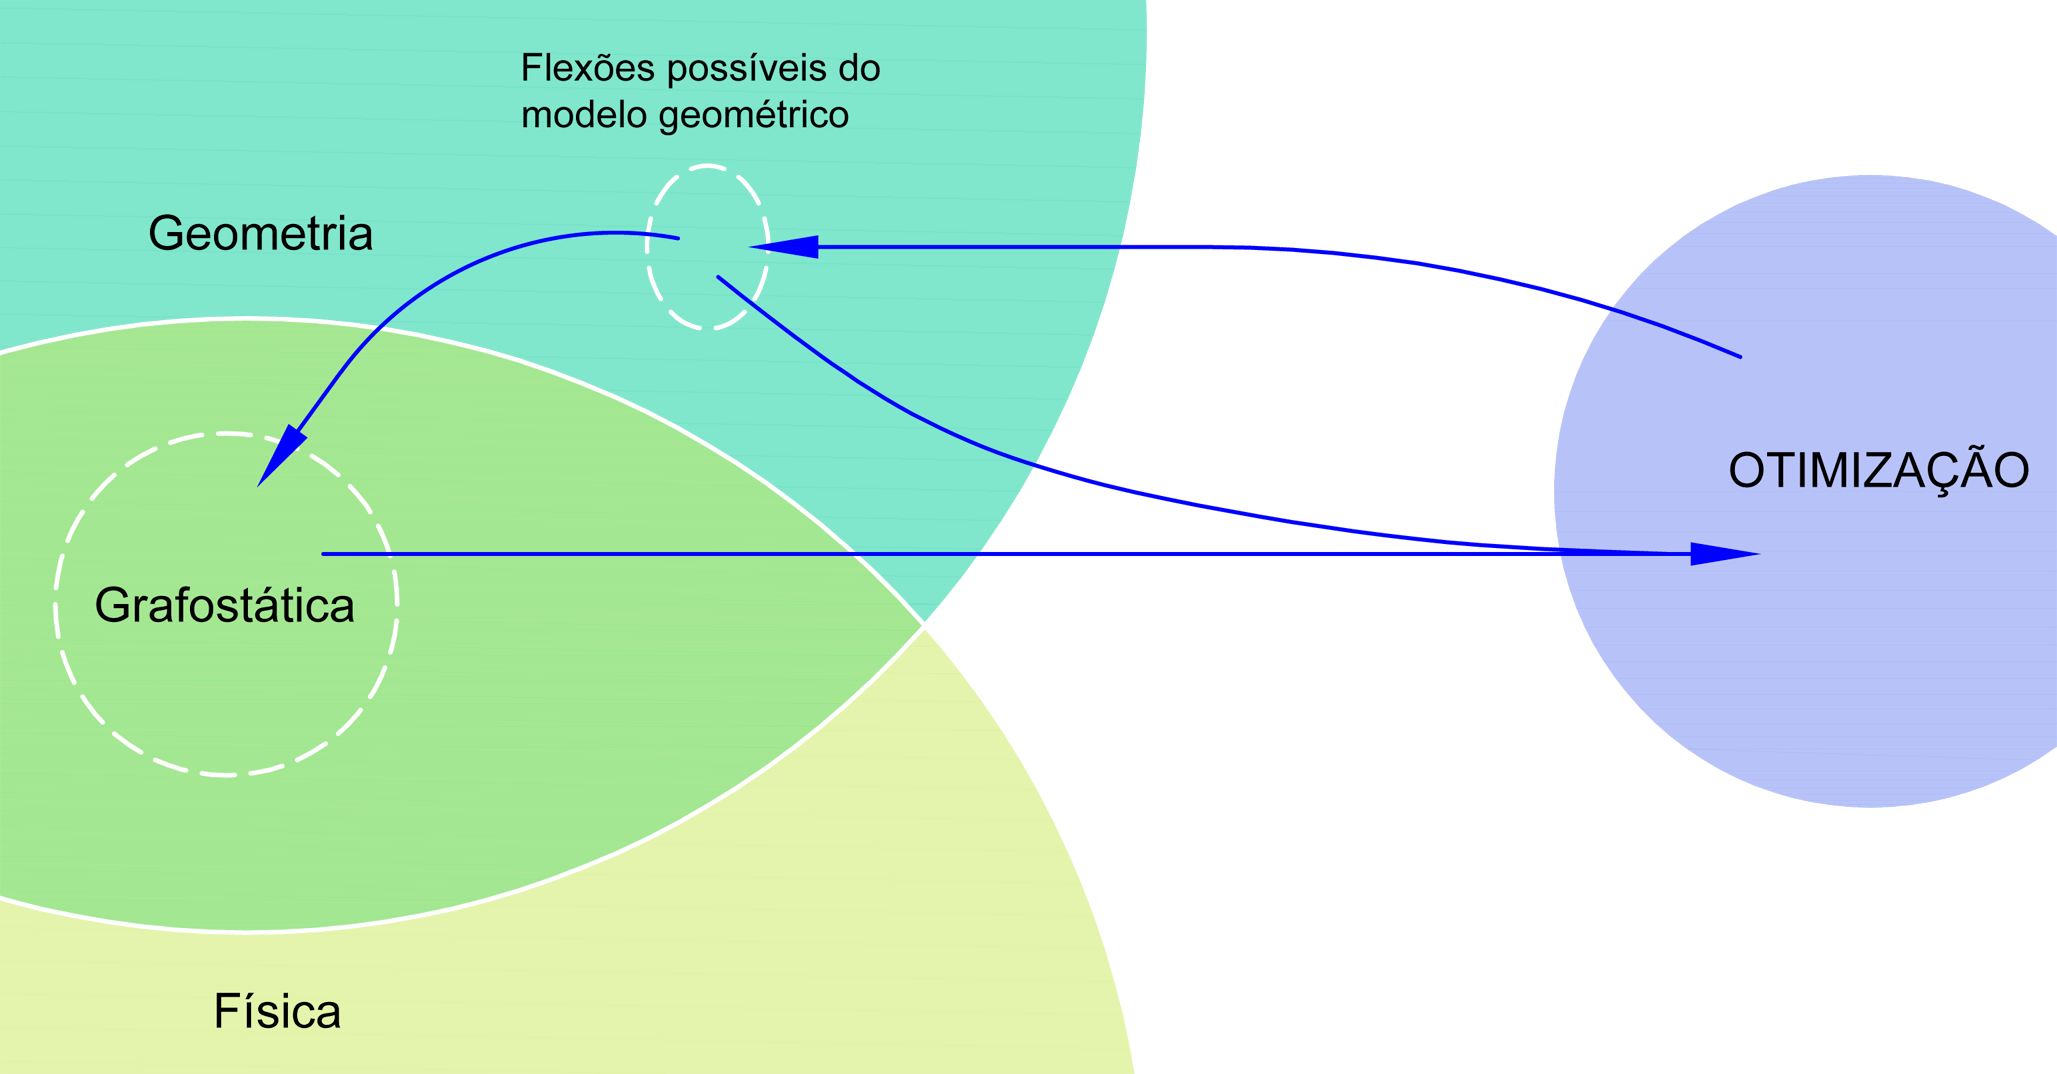
\includegraphics[width=0.9\textwidth]{modelo.png}
\caption{Modelo Te\'orico} \label{figura:mod}
\end{center}
\end{figure}

A primeira das partes do algoritmo, o modelo geom�trico baseado em par�metros e restri��es, corresponde no modelo te�rico �s "flex�es poss�veis do modelo geom�trico". Imaginemos um ret�ngulo ($L$x$P$) onde a medida de um dos lados � definida por uma vari�vel que representa um n�mero real variando entre 2 e 8. Alterando esse valor entre os limites estabelecidos a Figura � redesenhada para que a medita do referido lado corresponda ao valor da vari�vel. Para desenhar a outra dimens�o do ret�ngulo estabelece-se como regra que a �rea do pol�gono deve ser sempre igual a $10\quad unidades$. Para $L=2$, temos $P = \frac{10}{2} , \Rightarrow P = 5$. Para $L=8$, analogamente temos $P=1,25$, e assim para qualquer valor intermedi�rio ( $L=4 \Rightarrow P=2,5$; $L=3,2 \Rightarrow P=3,125$ ). A vari�vel que define o valor de $L$ � chamada de par�metro, e os valores limites desta e a obriga��o de ter-se sempre uma �rea $= 10 $ s�o denominados de restri��es e as altera��es nos valores das vari�veis produzem as flex�es do modelo.

A utiliza��o deste tipo de parametriza��o modifica o m�todo tradicional de projeto onde se prop�e o objeto, desenha, analisa e reprop�e. Aqui n�o se prop�e um modelo, mas um conjunto de par�metros e restri��es capaz de gerar uma s�rie de objetos para serem analisados como poss�veis solu��es para o problema. A etapa de an�lise n�o recai mais sobre um �nico objeto proposto, mas sobre uma gama de flex�es. Esta etapa pode levar tanto a uma reconfigura��o das vari�veis, quanto a redefini��o dos crit�rios de parametriza��o at� que conduza ao objeto final, eleito como solu��o do problema de projeto.

Esta abordagem auxilia o projetista a explorar uma gama maior de solu��es do que seria poss�vel pelo m�todo tradicional, principalmente quando os objetivos do projeto abrangem interesses subjetivos e criatividade \cite{krish2011}.

A an�lise de uma proposta de projeto pode ser feita unicamente pela t�cnica, experi�ncia e subjetividade do projetista, quanto pode contar com o aux�lio de ferramentas computacionais espec�ficas para alguns de seus aspectos. Um instrumento de avalia��o estrutural � implementado na segunda parte do algoritmo. As demais implica��es do problema podem ser avaliadas pelos crit�rios citados acima. Contudo, uma das grandes virtudes dos modelos baseados em  paramentos e restri��es � a velocidade com que se produzem varia��es na forma. Utilizando ferramentas de an�lise de desempenho � poss�vel realizar sucessivas simula��es, alterando a configura��o das vari�veis do SGP. Os resultados de cada uma destas simula��es podem contribuir com a experi�ncia do projetista para que as flex�es seguintes melhorem os desempenhos investigados.

O c�lculo e a an�lise de estruturas aparecem na ilustra��o do modelo te�rico (Figura \ref{figura:mod}) pertencendo zona de interse��o entre a F�sica e a Geometria. Com particular �nfase na Grafost�tica, descrita por \citeonline{baumgart2000} como:

\begin{quotation}
(...) um quase esquecido m�todo gr�fico intuitivo para a resolu��o de problemas mec�nicos (...) Era o m�todo Padr�o (...) usado por engenheiros civis pelo menos at� os anos 1940. Foi Gradualmente substituido por alternativas anal�ticas, principalmente por m�todos baseados na Tecnologia da Compuata��o.\footnote{\textit{Graphical statics is an almost forgotten, intuitive drawing method for solving plane mechanical problems."(...)"Graphical statics was the standard method for solving mechanical problems used by civil engineersmat least up until the 1940s. It was gradually replaced by analitical methods, especially methods based on computer tecnology.}}
\end{quotation}

O aspecto "quase esquecido" ser� contraposto no desenvolvimento desta disserta��o. Tendo em vista que, pelo aperfei�oamento da pr�pria Tecnologia da Computa��o, na medida em que esta ganhou profici�ncia na manipula��o e exibi��o de formas geom�tricas (Computa��o Gr�fica), autores e centros de pesquisa se interessaram pela Grafost�tica, dentre outros motivos pela natureza intuitiva do m�todo.

O m�todo de otimiza��o proposto, nada mais � do que a aplica��o de sucessivas flex�es ao modelo geom�trico, comparando os resultados �s suas correspondentes an�lises Grafost�ticas, aos aspectos est�ticos das formas resultantes e a antevis�o das demais caracter�sticas t�cnicas, funcionais, construtivas que a equipe de projeto, por seu estudo e experi�ncia seja capaz de enxergar.

Para um problema real de constru��o pode-se citar uma s�rie de vari�veis cuja quantifica��o � extremamente complexa ( aspectos est�ticos, a cultura construtiva, qualifica��o da m�o-de-obra local, etc). O m�todo tradicional de projeto, onde de uma proposi��o geral de uma forma passa por uma etapa  de questionamentos, altera��es e descartes, divide-se em elementos menores que passam pelo mesmo processo, at� que as solu��es de projeto sejam eleitas, oscila seus resultados entre sucessos e fracassos. A compet�ncia de uma equipe pode ser entendida, ainda que de maneira extremamente simplista, como a rela��o entra as ocorr�ncias de cada extremo desta oscila��o ao longo de sua atividade. As habilidades t�cnicas e a experi�ncia da equipe s�o diretamente ligadas aos relativos �xitos e insucessos, seja no m�todo tradicional ou qualquer outro.

Os SGP proporcionam uma metodologia expressivamente mais r�pida de se alterar as formas em estudo, possibilitando a experimenta��o de uma gama maior de varia��es, dentre as poss�veis solu��es, podendo recorrer diretamente � crit�rios de escolha utilizados pelo m�todo tradicional sobre uma quantidade maior de propostas.   
 
\subsection{Objeto de Estudo}
\label{subsection:objetodeestudo}

\begin{figure}[!ht]
\begin{center}
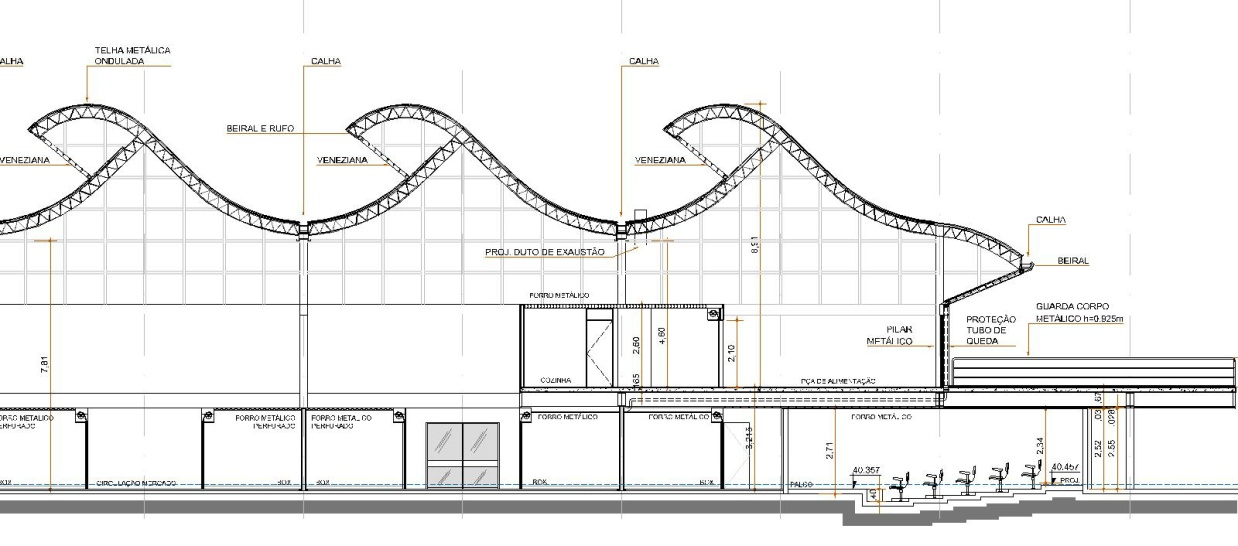
\includegraphics[width=0.9\textwidth]{cortemercado.png}
\caption{Proposta para o Mercado S�o Miguel - Autoria: Jo�o Filgueiras Lima e Instituto Habitat - Trecho do "Corte AA"\ - Fonte: Acervo do Instituto Habitat} \label{figura:ctmercado}
\end{center}
\end{figure}

O obejeto de estudo eleito foi uma treli�a de sustenta��o de coberturas do tipo \textit{\textbf{shed}} com inspira��o nas treli�as met�licas recorrentemente apresentadas na obra do arquiteto Jo�o (Lel�) Filguiras Lima. No exemplo mostrado na Figura \ref{figura:ctmercado} v�-se um trecho de um corte da proposta para a requalifica��o do Mercado S�o Miguel em Salvador - Ba.

O interesse pelos \textit{\textbf{sheds}} vem destes serem, al�m de estruturas de suporte de coberturas, elementos de ilumina��o e ventila��o capazes de melhorar substantivamente o conforto do ambiente para o uso humano, e assim diminuindo o consumo de energia com ilumina��o e climatiza��o do espa�o. Muito utilizados em projetos de grandes galp�es e plantas industriais.

A inspira��o na citada obra procura trazer o apuro est�tico que acompanham as solu��es tecnicamente embasadas que marcam de forma singular o trabalho de um dos mais importantes arquitetos brasileiros, trazendo mais complexidade ao experimento.

Aplicando o Modelo Te�rico e as partes do algoritmo ao objeto de estudo, o que se prop�e � um SGP formado por um modelo baseado em par�metros e restri��es capaz de produzir alternativas de projeto para uma treli�a de um \textit{\textbf{shed}}. Este modelo deve levar em conta que as vari�veis devem sintetizar uma forma de desenho onde a criatividade e outros aspectos subjetivos do projeto tenham espa�o para emergir no processo\ \cite{shea2005}. Uma ferramenta de an�lise estrutural capaz de calcular as tens�es atuantes em cada um dos elementos das diversas configura��es poss�veis do modelo geom�trico, sendo baseada majoritariamente em mecanismos da Grafost�tica.

%Nesta se\c{c}\~ao o problema \'e claramente identificado. Deve-se
%apresentar os argumentos que levaram \`a identifica\c{c}\~ao do
%problema que ser\'a trabalho. Alguns autores podem ser citados com
%o prop\'osito de explicitar a preocupa\c{c}\~ao da comunidade
%cient\'ifica ou de parte dela, em tentar resolver o problema
%dentro dos \^ambitos estabelecidos.

\section{Objetivos}
\label{section:objetivo}

O objetivo geral deste trabalho �:

\begin{itemize}
\item Analisar a viabilidade pr�tica da utiliza��o dos SGP na atividade de projeto arquitet�nico.
\end{itemize}

Como Objetivos espec�ficos temos:
\begin{itemize}
\item Implementar um SGP para atuar como ferramenta de aux�lio no projeto da cobertura de um \textit{\textbf{shed}};
\item Comprovar a eficacia dos SGP na elabora��o de solu��es de projeto onde aspectos subjetivos s�o parte integrante do problema;
\item Repensar as virtudes da Grafost�tica como instrumento de an�lise estrutural, ressaltando seu aspecto intuitivo e pr�tico. 
\end{itemize}


%Nesta se\c{c}\~ao os objetivos principal e espec\'ificos (tamb\'em
%pode-se se utilizar a palavra meta) da monografia de
%gradua\c{c}\~ao ou especializa\c{c}\~ao, disserta\c{c}\~ao de
%mestrado ou tese de doutorado s\~ao apresentados.



\section{Import\^ancia da Pesquisa}
\label{section:importanciapesquisa}

\citeonline{kolarevic2003} relata que o distanciamento entre o planejamento e a execu��o na \textbf{ICC} gradativamente transformou a Arquitetura em "(...)uma profiss�o incerta quanto ao seu papel na sociedade contempor�nea e sua economia, e uma profiss�o incapaz de responder aos desafios da Era da Informa��o."\footnote{\textit{The outcome of this progressive disassociation of architecture  from the rest of the building industry is a professsion unsure of its role in contemporary society and it�s economy, and a profession unable to respond to the challenges and opportunities of the Information Age.}} Entretanto aponta, com bastante otimismo que:

\begin{quotation}
Nos novos processos de produ��o assistidos por computador, projeto e constru��o n�o s�o mais dom�nios separados(...)Construtores e fabricantes se envolveram nas primeiras fases do projeto e os arquitetos participam ativamente em todas as fases da constru��o.\footnote{\textit{In the digitelly-driven processes of production, design and construction are no longer separate realms but are instead , fluidly amalgamated.Builders and fabricators become involved in the earlies phases of constructions and architects aactively participate in all phases of construction.}}
\end{quotation}

\citeonline{Florio2011} constata que uma semelhante "Fragmenta��o do ensino em disciplinas estanques, sem conex�es umas com as outras, sempre gerou s�rios problemas para a integra��o com os conte�dos no curr�culo." E encontrou em atividades de modelagem param�trica desenvolvidas entre estudantes de Arquitetura uma resposta animadora no encurtamento destas dist�ncias.

E inevit�vel imaginar o quanto as disrupturas sentidas na pr�tica e no ensino est�o relacionadas. A natureza interdisciplinar da aplica��o dos SGP se evidencia em ambos os casos. Os benef�cios apontados recaem n�o somente sobre a profiss�o de arquiteto, trabalha-se com a esperan�a de levar as virtudes da interdisciplinaridade � \textbf{ICC} como um todo.

O experimento desenvolvido aqui, embora calcado especialmente na etapa de projeto, procura trazer uma contribui��o pontual no corrente debate.

Entre tantos desempenhos que poderiam ser escolhidas como objetivo da segunda parte do algoritmo, os argumentos favor�veis � estrutura partem da base do que chamamos de Arquitetura. Vitr�vio, autor do mais antigo tratado arquitet�nico conhecido pela Hist�ria (10 volumes, aprox. 27 a 16  A.C.), embasou a teoria e pr�tica da atividade em 3 pilares:

\begin{itemize}
\item Firmitas
\item Utilitas
\item Venustas
\end{itemize}

O terceiro pilar refere-se � est�tica da obra. O segundo sobre o uso. A atividade fim para qual a constru��o foi dedicada, bem como toda e qualquer apropria��o humana que ali ocorra. O primeiro est� ligado � propriedade do edif�cio de permanecer inteiro. � no espa�o formado por elementos capazes de se portar que qualquer uso pode ocorrer e qualquer teoria est�tica sobre a Arquitetura pode ser levantada. No caso dos \textit{\textbf{sheds}}, o benef�cio que pode ser alcan�ado, por exemplo, pela exaust�o do "ar quente" pela abertura superior, precisa em primeiro lugar que a solu��o estrutural seja poss�vel.

A Grafost�tica aparece como uma ferramenta proposta para o entendimento dos prolemas estruturais. \citeonline{gerhardt2003} defendem o valor dos m�todos gr�ficos no ensino da estrutura para engenheiros porque estes permitem que se experimente visualmente as inter-rela��es entre, por exemplo, a geometria da estrutura e as for�as atuantes. Relatam tamb�m a aplica��o do m�todo para um estudo de refor�o estrutural visando atender uma mudan�a de uso para um dos espa�os do pr�dio da prefeitura de Berlim. Aplicou-se simplesmente um programa CAD e o conhecimento do m�todo. Os m�todos anal�ticos relacionam express�es matem�ticas � formas geom�tricas, as vantagens cognitivas de se aplicarem formas geom�tricas para avaliar a solidez de outras formas geom�tricas s�o defendidas pelos autores. A interse��o de duas retas tem por equivalente anal�tico a resolu��o de um sistema de duas equa��es com duas inc�gnitas. O CAD funciona como uma calculadora geom�trica extremamente interessante para a tarefa: Al�m de  fazer parte do cotidiano profissional dos projetistas, promove uma liga��o entre diferentes disciplinas ligadas � constru��o.

\begin{figure}[!ht]
\begin{center}
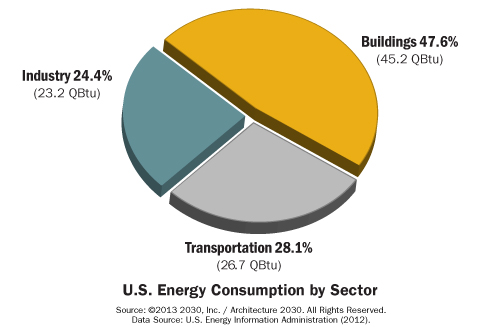
\includegraphics[width=0.70
\textwidth]{energybysector.jpg}
\caption{Consumo de Energia - Gr�fico produzido pela ONG Architecture 2030. Com base nos dados coletados pela ag�ncia U.S. Energy Information Administration (EIA) referentes ao ano de 2012}
\label{figura:consumoenergetico}
\end{center}
\end{figure}

A relev�ncia do estudo e aplica��o dos m�todos de otimiza��o na ICC est� diretamente ligada ao crescimento da for�a que as preocupa��es ecol�gicas e de conserva��o de energia ganharam. O papel a ser desempenhado pela Ind�stria da Constru��o neste cen�rio n�o � pequeno. A Figura  \ref{figura:consumoenergetico} apresenta um gr�fico elaborado pela ONG \textit{Architecture 2030} a partir de dados coletados pela ag�ncia \textit{U.S. Energy Information Administration} (EIA) sobre o consumo de energia nos EUA dividindo-o em tr�s setores: a ind�stria, o transportes e os edif�cios. A esse �ltimo setor cabe a maior das parcelas, acumulando quase a metade da energia consumida no pais ($ 47,6 \% $). A contribui��o que a otimiza��o por SGP pode oferecer � defendida por \citeonline{krish2011}:
\begin{quotation}
Os SGP, por outro lado, tem a capacidade de operar nas fases conceituais do projeto, quando a este ainda est� sendo formulado. A habilidade de explorar varia��es nestes primeiros est�gios pode produzir benef�cios muito maiores  que a otimiza��o realizada entre limites estreitos nas fases finais do processso.\footnote{\textit{Generative design on the other hand, can operate at the conceptual stages of design,where the design is still under formulation. The ability to explore design variations at the early stages of design can produce far more beneficial results, than optimizing it within narrow means at the final stages of design.}}
\end{quotation}
%O pesquisador/estudante deve apresentar os aspectos mais
%relevantes da pesquisa ressaltando os impactos (e.g. cient\'ifico,
%tecnol\'ogico, econ\^omico, social e ambiental) que a pesquisa
%causar\'a. Deve-se ter cuidado com a ingenuidade no momento em que
%os argumentos forem apresentados.



%\section{Motiva\c{c}\~ao}
%\label{section:motivacao}

%Muito associada \`as se\c{c}\~oes \textbf{Defini\c{c}\~ao do
%problema} e \textbf{Import\^ancia da pesquisa}, esta se\c{c}\~ao,
%apesar de ser opcional, pode ser relevante principalmente em se
%tratando de projetos de disserta\c{c}\~oes de mestrado e teses de
%doutorado. Pode-se apresentar motiva\c{c}\~oes pessoais, baseadas
%em dados e em interesses do(s) centro(s) de pesquisa onde se
%est\'a desenvolvendo o projeto.



\section{Limites e Limita\c{c}\~oes}
\label{section:limiteslimitacoes}

Uma s�rie de quest�es deve ser levada em conta na implementa��o do experimento proposto neste trabalho de pesquisa. Quanto a an�lise de estruturas vale dizer que, salvo poucas exce��es (e.g. c�lculo de estruturas pelo m�todo dos elementos finitos planos e espaciais), trabalha-se com simplifica��es das formas onde linhas de eixo representam elementos tridimensionais a serem dimensionados. O que j� representa uma simplifica��o, apesar de estar na base da teoria das estruturas.

Uma s�rie de outras simplifica��es foram tomadas quanto as estruturas analisadas pelo trabalho que ser�o apresentadas a medida que o experimento � descrito. � importante entender contudo que a exequibilidade de uma estrutura depende tanto da sua an�lise e dimensionamento quanto do seu detalhamento. Uma simples liga��o entre elementos construtivos mal estudada, um erro de soldagem pode levar ao colapso do conjunto.

Os SGP s�o em si um exec�cio de limites e possibilidades. � desej�vel que os algoritmos sejam capazes de produzir uma gama de solu��es fact�veis. A natureza de como eles s�o constru�dos, baseando-se em par�metros e restri��es, por si j� subentende-se que cada algoritmo trabalha dentro de suas pr�prias limita��es. Cria-se um territ�rio de fronteiras demarcadas mas que deve ser vasto o suficiente para que aconte�a uma satisfat�ria investiga��o do que nele pode estar contido.

Embora o pressuposto da pesquisa seja de propor um m�todo de trabalho aplic�vel em projetos reais, onde estruturas fact�veis possam ser propostas e modificadas, dentro de uma estrat�gia compat�vel com os recursos e prazos usuais em um escrit�rio de projetos, a pesquisa n�o trata de um projeto espec�fico. Isso explicita que, no desenvolvimento do experimento, n�o se conhece o contexto em que uma solu��o da treli�a vai ser escolhida. Sem o programa da edifica��o e o uso destinado, o v�o entre apoios n�o pode ser determinado. Sem as informa��es sobre o clima do local de implanta��o do projeto, a orienta��o, o regime de chuvas, etc; a necessidade de maior ou menor exaust�o n�o pode ser analisada. A rela��o entre est�tica e custo tamb�m precisaria de mais dados para nortear uma investiga��o da forma. O que se apresenta no trabalho � um m�todo de projeto suficientemente vers�til para se adaptar as demandas de diversas edifica��es que admitam algumas das treli�as contidas nas flex�es do SGP como solu��es de cobertura.

Ao tratar de um SGP que procura valorizar os atributos est�ticos do desenho, faz-se necess�rio ressaltar que a Filosofia das Artes � um campo de estudo espec�fico e vasto. Qualquer investiga��o neste campo demanda um investimento de tempo, conceitualiza��o e literatura espec�fica que ultrapassam o escopo da presente pesquisa. 
%Nesta se\c{c}\~ao o pesquisador apresenta os limites e
%limita\c{c}\~oes definidas antes e e durante o desenvolvimento da
%pesquisa. Assim, o trabalho fica resguardado de poss\'iveis
%cr\'iticas. Os limites s\~ao aspectos que estabelecem o escopo da
%pesquisa e as limita\c{c}\~oes s\~ao os problemas enfrentados
%durante a pesquisa que levam a tomadas de decis\~ao que podem,
%inclusive, mudar o direcionamento da pesquisa.

\section{Quest\~oes e Hip\'oteses}
\label{section:questoeshipoteses}

Como os SGP podem contribuir nas fases iniciais da concep��o das formas de um projeto arquitet�nico?

Esta � a principal quest�o investigada por esta pesquisa. Quanto �s hip�teses, imagina-se que � poss�vel desenvolver um SGP que sirva como uma ferramenta � ser usada por equipes de Arquitetura que seja: 

\begin{itemize}
\item de intera��o direta com o desenho, o tra�o e os aspectos est�ticos da cria��o;
\item forne�a subsidio para um julgamento t�cnico da forma que emerge do processo  de projeto;
\item apresente uma forma pr�tica de alterar, estudar e eleger uma solu��o.
\end{itemize}

Investiga-se tamb�m a hip�tese de que a implementa��o do algoritmo de an�lise baseado na Grafost�tica apresenta mecanismos semelhantes e compat�veis com os utilizados na constru��o de um SGP, e apresenta vantagens, do ponto de vista cognitivo, em rela��o aos seus an�logos anal�ticos. 

%Esta \'e uma se\c{c}\~o importante, pois nela as quest\~oes feitas
%a partir da defini\c{c}\~ao do problema (comentada na Se\c{c}\~ao
%\ref{section:definicaoproblema}) s\~ao explicitamente expressadas,
%conduzindo \`a n\~ao menos expl\'icita, hip\'otese (ou
%hip\'oteses) que ser\'a investigada, aceita ou rejeitada.

\section{Aspectos Metodol\'ogicos}
\label{section:aspectosmetodologicos}

Lan�ando m�o de uma metodologia experimental, a organiza��o geral do algoritmo baseou-se no fluxograma proposto por \citeonline{bohnacker2012}, mostrado na Figura \ref{figura:fluxogramametodologia}. Pode-se ver no diagrama as etapas de concep��o e funcionamento de um SGP al�m de ilustrar a maneira como a otimiza��o ocorre, sempre atrav�s do julgamentos do projetista (\textit{Designer}). 

\begin{figure}[!ht]
\begin{center}
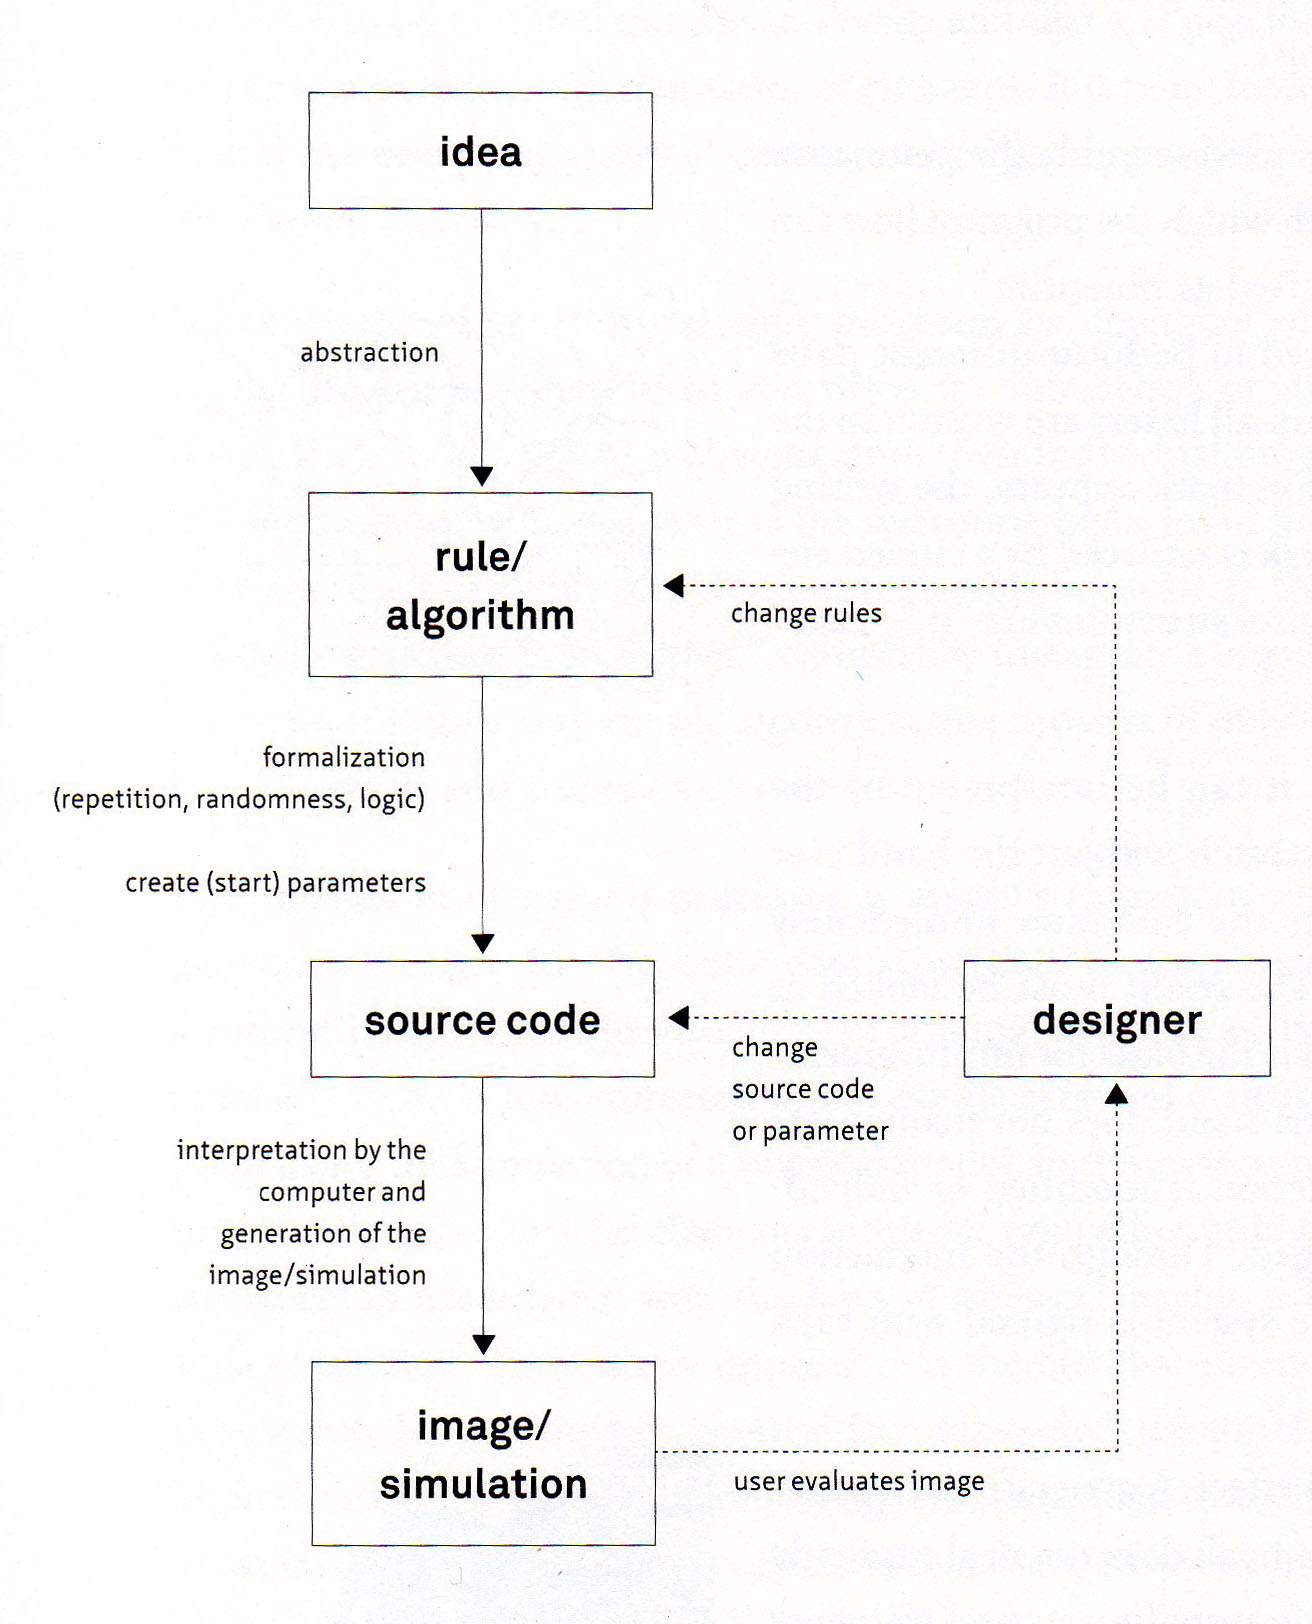
\includegraphics[width=0.75\textwidth]{fluxogramametodologia.jpg}
\caption{Fluxograma de um SGP - fonte: \citeonline{bohnacker2012}}
\label{figura:fluxogramametodologia}
\end{center}
\end{figure}

A valida��o dos resultados segue crit�rios espec�ficos para cada uma das partes do algoritmo apresentadas na Se��o \ref{section:definicaoproblema}:

No caso do modelo geom�trico baseado em par�metros e restri��es, vistas as limita��es quanto a aprecia��o dos aspectos est�ticos, ser�o avaliadas as capacidades de produzir varia��es. A facilidade e velocidade com que essas transforma��es ocorrem. A praticidade da utiliza��o dessas ferramentas no cotidiano do projetista.

O algoritmos de an�lise Grafost�tica deve ser constru�do de maneira coerente com os m�todos desta, bem como da Mec�nica dos S�lidos e Resist�ncia dos Materiais. Os resultados obtidos ser�o validados pela coer�ncia dos gr�ficos gerado pelo algoritmo com a teoria e regras da Grafost�tica, t�cnica de c�lculo reconhecida e matematicamente provada pelos tratados de \citeonline{cremona1890graphical}.

O m�todo de otimiza��o passa, inevitavelmente, pelo julgamento do projetista. A rela��o entre pl�stica e economia assume diferentes pesos e prefer�ncias de acordo com �s opini�es de cada projetista e a finalidade de cada projeto. Para que esse julgamento seja feito � preciso assegurar que as informa��es de forma e an�lise estrutural sejam coerentes, que a r�pida altera��o de uma implique numa tamb�m veloz e coerente altera��o de outra, e que o conjunto opere sem conflitos entre as partes.

%Aqui devem ser apresentados as assun\c{c}\~oes do pesquisador com
%rela\c{c}\~ao \`as perspectivas filos\'oficas, aos m\'etodos de
%pesquisa utilizados e aos modos de an\'alise. Assim, ainda que
%apresente resultados ou achados pol\^emicos, a pesquisa poder\'a
%ser validada, pois estar\'a consistente e apresentar\'a uma
%coer\^encia com as assun\c{c}\~oes do pesquisador.

%Quando para a pesquisa \'e muito importante ressaltar os
%fundamentos metodol\'ogicos, sugere-se escrever ou transformar
%esta se\c{c}\~ao em um cap\'itulo espec\'ifico.



\section{Organiza��o da Disserta��o de Mestrado}
\label{section:organizacao}

Este documento apresenta $6$ cap�tulos e est\'a estruturado da
seguinte forma:

\begin{itemize}

  \item \textbf{Cap\'itulo \ref{chapter:introducao} - Introdu\c{c}\~ao}: contextualiza o \^ambito, no qual a
  pesquisa proposta est\'a inserida. Apresenta, portanto, a
  defini\c{c}\~ao do problema, objetivos e justificativas da pesquisa e
  como esta \thetypeworkthree est\'a estruturada;

  \item \textbf{Cap\'itulo \ref{chapter:sistemasgenerativosdeprojeto} - Sistemas Generativos de Projeto}: apresenta o conceito de algoritmo, investiga o significado dos algoritmos generativos e apresenta os principais modelos dos AGs aplicados ao projeto arquitet�nico;

  \item \textbf{Cap\'itulo \ref{chapter:grafostatica} - Grafost�tica}: apresenta os fundamentos do m�todo, os procedimentos de c�lculo de treli�as utilizados na implementa��o do algoritmo de an�lise estrutural, as pesquisas em que este vem sendo atualmente aplicado, os \textit{sotftwares} que utilizam, e um breve levantamento da pesquisa bibliogr�fica, citando alguns algoritmos apresentados nos manuais pr�ticos da Est�tica Gr�fica;

  \item \textbf{Cap\'itulo \ref{chapter:ambientedeimplementacao} - ambiente de Testes do Algoritmo}: uma r�pida apresenta��o do ambiante computacional onde o experimento foi realizado;

  \item \textbf{Cap\'itulo \ref{chapter:trabalhoexperimental} - Implementa��o do Experimento}: apresenta como os algoritmos que formam o SGP foram criados, como funcionam, como se estabelece a comunica��o entre eles, e como podem ser utilizados na explora��o das poss�veis solu��es de projeto;

  \item \textbf{Cap\'itulo \ref{chapter:consideracoesfinais} - Conclus�es}: apresenta as conclus\~oes, contribui\c{c}\~oes
  e algumas sugest\~oes de atividades de pesquisa a serem desenvolvidas no futuro.

\end{itemize}

    % !TeX encoding = ISO-8859-1
% !TeX spellcheck = pt_BR
\chapter{Algoritmos Generativos e Sistemas Generativos de Projeto}
\label{chapter:sistemasgenerativosdeprojeto}

\begin{flushright}
  \textit{"A man provided with paper, \\pencil, and rubber,\\ and subject to strict discipline,\\ is in effect a universal machine."}
  \\
  (Alan Turing)
\end{flushright}

Os componentes essenciais de um SGP s�o: os algoritmos generativos e o ambiente computacional onde estes ser�o executados. Envolvendo os sistemas operacionais, os programas, as linguagens de programa��o, os computadores e demais dispositivos empregados (\textit{hardware}) e as interfaces com usu�rios, os ambientes de implementa��o s�o correspons�veis pelos limites e possibilidades entre os quais operam os SGP. No caso espec�fico desta pesquisa, a praticidade de se gerar formas em um ambiente CAD utilizado no mercado de desenho de projetos, a capacidade de se implementar algoritmos de maneira r�pida e eficiente, e a facilidade de ver os resultados das altera��es dos par�metros em tempo real, tiveram grande import�ncia na escolha. J� os Algoritmos Generativos determinam principalmente a l�gica que rege a cria��o de formas. As caracter�sticas b�sicas do ambiente computacional escolhido s�o apresentadas no Cap�tulo \ref{chapter:ambientedeimplementacao}. As defini��es, conceitos e principais os modelos computacionais dos AG aplicados � Arquitetura formam o conte�do deste cap�tulo.


\section{Defini��o de Algoritmo e Algoritmos Generativos}
\label{section:definiAlgor}

A palavra "algoritmo" tem sua origem no nome do matem�tico e astr�nomo �rabe Mohammed ibu-Musa al-Khowarizmi (s�culo VII). A tradu��o latina de um de seus livros, sobre a "arte hindu de calcular", foi respons�vel por difundir o sistema de numera��o que chamamos de hindu-ar�bicos na Europa. Embora n�o revindicasse a autoria do sistema, a "nova" nota��o, come�ou a ser referida como a de "al-Khowarizmi" ou "algorismi" e posteriormente "algorismo" ou "algoritmo". Com o passar do tempo a palavra "algoritmo" passou a significar processo, regra, m�todo (e.g. O algoritmo de Euclides para encontrar o m�ximo divisor comum de um n�mero) \cite[p. 166]{boyer1974}.

\citeonline[p. 1-8]{knuth1997art} define o conceito atual do termo como um conjunto finito de regras que fornece uma sequ�ncia de opera��es para a solu��o de um problema espec�fico, e que deve atender cinco requisitos:

\begin{itemize}  
\item{Finitude}  
\item{Precis�o}  
\item{Entrada de Informa��o}
\item{Sa�da de Informa��o}
\item{Efetividade} 
\end{itemize}

Em conson�ncia com os assuntos abordados por esse trabalho, na fun��o de ilustrar o conceito, foi escolhido um exemplo de algoritmo proveniente da geometria e desenho t�cnico, em lugar de uma abordagem puramente num�rica: o m�todo de divis�o de uma seguimento de reta $\overline{AB}$ qualquer em uma quantidade finita de seguimentos iguais, representada pelo n�mero inteiro $N$. O processo � realizado com  �xito seguindo os cinco passos da "receita" descrita abaixo e representados graficamente na Figura \ref{figura:algorEg}:

\begin{enumerate}  
\item{Dado o segmento de reta $\overline{AB}$ desenhar, a partir do ponto A, uma semi-reta n�o paralela � $\overline{AB}$.}  
\item{Dado o n�mero $N$ de divis�es, utilizando o compasso com uma mesma abertura qualquer,  partindo do ponto $A$, marcar $N$ pontos consecutivos e equidistantes sobre a semi-reta tra�ada no passo anterior.}  
\item{Tra�ar um segmento unindo o "N-�simo" ponto marcado no passo anterior com a extremidade B do segmento $\overline{AB}$.}
\item{ Tra�ar paralelas ao segmento desenhado no passo 3, passando pelos pontos definidos no passo 2 e interceptando o segmento de reta $\overline{AB}$.}
\item{FIM} 
\end{enumerate}

\begin{figure}[!ht]
\begin{center}
  \mbox{
      \subfigure[Dados Iniciais]
         {
            \label{figura:algorEgP0}
            \includegraphics[width=0.40\textwidth]{algorEgP0.png}
         }
  }
  \mbox{
      \subfigure[Passo 1]
         {
            \label{figura:algorEgP1}
            \includegraphics[width=0.45\textwidth]{algorEgP1.png}
         }
  }


\mbox{
      \subfigure[Passo 2]
         {
            \label{figura:algorEgP2}
            \includegraphics[width=0.45\textwidth]{algorEgP2.png}
         }
  }
  \mbox{
        \subfigure[Passo 3]
           {
              \label{figura:algorEgP3}
              \includegraphics[width=0.45\textwidth]{algorEgP3.png}
           }
    }
    
    \mbox{
          \subfigure[Passo 4]
             {
                \label{figura:algorEgP4}
                \includegraphics[width=0.45\textwidth]{algorEgP4.png}
             }
      }
\end{center}
\caption{Exemplo de algoritmo - subdivis�o de um seguimento em um n�mero finito (5) de partes iguais}
\label{figura:algorEg}
\end{figure}

Comparando o exemplo com a defini��o acima, nota-se que o m�todo de divis�o de segmentos tem um fim. A precis�o diz respeito a clareza das instru��es que, no caso citado, s�o suficientemente claras para o entendimento humano. Por entrada de informa��es temos o n�mero inteiro de divis�es e o objeto seguimento de reta $\overline{AB}$. Por sa�da podemos considerar os pontos que dividem o seguimento em $N$ partes ou os $N$  seguimentos de reta justapostos sobre o seguimento $\overline{AB}$. E a efetividade, a capacidade de lograr �xito na execu��o do seu prop�sito, pode ser aferida analisando a Figura \ref{figura:algorEgP4} comparada com o teorema descrito por Tales: um feixe de paralelas cortado por duas transversais quaisquer as divide em seguimentos proporcionais.

O pioneiro dos sistemas generativos de projeto aplicados � Arquitetura, William J. \citeonline[p.61-64]{mitchell2008} afirma que todo o trabalho de desenho geom�trico/t�cnico � fundamentado em algoritmos (e.g. os m�todos descritos em "Os Elementos" de Euclides). O vocabul�rio algor�tmico do desenho � absorvido pelo projetista e, pela combina��o de uma gama de procedimentos, v�o surgindo n�o s� formas gradativamente mais elaboradas, como uma linguagem t�cnica do desenho de projetos. Palavras como perpendicular, paralela, ponto central, tangente, etc passam a resumir uma s�rie de instru��es e descrever algoritmos inteiros. Nos prim�rdios do projeto assistido por computador, esse era o papel dos programadores: A transposi��o dos algoritmos de desenho para o ambiente digital.



Os Algoritmos Generativos s�o um campo de estudo novo e, embora estejam sendo abra�ados pelos grandes escrit�rios de Arquitetura do mundo e estejam sendo estudados e ensinados em muitos centros acad�micos de Arquitetura \cite{krish2011}, ainda est� a procura de uma defini��o clara e completa. A simples formula��o de que s�o algoritmos voltados a gera��o de forma, cai por terra pelo simples falto de todo o desenho t�cnico ser constru�do a partir de algoritmos.

A simples transcri��o dos algoritmos de desenho a ferramenta computacional tamb�m n�o � suficiente para definir o termo. Em seguida, partiu-se para novos dom�nios como relatado no mesmo texto de \citeauthoronline{mitchell2008}:

\begin{quotation}
(...) Com o apoio das habilidades de programa��o mais do que inventividade mec�nica, programadores gr�ficos primeiro replicaram as fun��es de instrumentos de desenho tradicional, depois foram muito al�m. Isso disponibilizou para os projetistas um ainda maior vocabul�rio gr�fico junto com uma sintaxe mais elaborada - em suma, uma mais rica e potencialmente mais expressiva linguagem gr�fica e espacial.\footnote{\textit{Relying upon software skills rather than mechanical ingenuity, graphics programmers first replicated the functions of traditional drafting instruments, and then went far beyond them. This has made a wider graphic vocabulary available to designers, together with a more elaborate syntax?in all, a richer and potentially more expressive graphic and spatial language.}}  
\end{quotation}

\citeonline[p. 37-64]{terzidis2006algorithmic} classifica os problemas de projeto como: pass�veis de solu��o (\textit{problem-solving}), referindo-se ao conceito tradicional de encontrar um caminho entre os pontos $A$ e $B$, ou de abordagem (\textit{problem-adressing}). Problemas como a forma inicial, est�tica ou planejamento n�o tem uma solu��o definitiva, mas estrat�gias de trabalho que podem atingir resultados mais ou menos satisfat�rios. Para o autor, projetar � uma forma de pensar. � uma atividade intrinsecamente atada as caracter�sticas mais existencialmente humanas como a l�gica, criatividade e identidade. E acaba por conferir � certos algoritmos a capacidade de explorar al�m, em paralelo ou no lugar de maneiras tradicionais e estabelecidas de se pensar o projeto.

\citeonline{DIno2012} elenca quatro caracter�sticas presentes nos AG: Os par�metros de entrada, os mecanismos generativos (regras e algoritmos), a gera��o de varia��es de formas (sa�da), e a escolha da melhor varia��o. Os dois primeiros requisitos est�o presentes de maneira id�ntica na defini��o de algoritmo, os outros est�o mais ligados � forma de aplica��o das ferramentas. Gerar uma sa�da de dados processados � tamb�m uma caracter�stica  dos algoritmos. Entradas diferentes produzem sa�das variantes em qualquer problema, trabalhar com varia��es e escolher entre estas, como � pontuado nos dois �ltimos requisitos, fazendo com que as propriedades de um AG diferenciem-se das caracter�sticas b�sicas de um algoritmo apenas por uma maior especificidade no que diz respeito ao modo de utiliza��o da ferramenta.

Em suma, os autores concordam que, al�m da gera��o de formas, os Algoritmos Generativos possibilitam a aplica��o de uma metodologia diferente de trabalho. Parte importante do que caracteriza um AG � a possibilidade de se escolher uma solu��o de projeto a partir da variabilidade gerada pelos par�metros e regras. O desafio te�rico, que esta pesquisa n�o encontrou resposta definitiva, � formular uma defini��o mais precisa, que abarque as referidas novas formas de se trabalhar e eleger uma solu��o de projeto.


\section{Principais Modelos de Algoritmos Generativos Aplicados � Arquitetura e ICC}
\label{section:tiposag}

Os AG s�o sim algoritmos capazes de gerar formas, mas tamb�m de trazer algo novo para esse antigo jogo. Procurando revelar mais sobre a natureza destes m�todos, uma lista dos principais tipos de AGs e algumas de suas aplica��es na Arquitetura aparece como o caminho eficaz. Algumas revis�es de literatura serviram como base para a elabora��o desta lista (\citeonline{ fasoulaki2008}; \citeonline{Santos2009}; \citeonline{daly2009}; \citeonline{Singh2012}), bem como artigos fundamentais e atuais sobre os diversos modelos utilizados. Aplica��es dos principais algoritmos foram buscados tanto nos artigos cient�ficos quando em projetos constru�dos e propostas. 

Curiosamente a maioria desses m�todos tem rela��o direta com aspectos da natureza, a fonte de inspira��o dos primeiros construtores, dotados apenas da geometria que estavam formulando e de instrumentos rudimentares de desenho e constru��o, e repetidamente interpretada por todas as gera��es de projetistas. No "Ensaio sobre a Arquitetura" de 1753, o Abade Laugier revisita o conceito fundamental da "cabana primitiva", quatro pilares de trocos de �rvore suatentando uma cobertura r�stica de duas �guas. Uma apologia � simplifica��o das formas. Segundo \citeonline[p. 5]{frampton2000}, foi um ponto crucial na sucess�o de fatos que nos levam ao lema "ornamento � crime" do arquiteto Adolf Loos no in�cio do s�culo XX. Um elo na cadeia de eventos que transformou as formas detalhadamente esculpidas de colunas cl�ssicas em s�lidos plat�nicos como o cilindro e o prisma. Por�m o que grande parte dos m�todos aqui apresentados explora s�o justamente os elementos que o platonismo, a Geometria, as ci�ncias e a Arquitetura tinham deixado de lado, e que passaram a ser discutidos cientificamente pelos estudos relacionados com o fim do modelo mecanicistas do universo (Sistemas Complexos, Teoria do Caos Determin�stico, etc).

\subsection{Gram�ticas de Forma (GF)}
\label{subsection:agGF}

Introduzido por George Stiny e James Gips em 1971 \cite{stiny1972} nos campos da Pintura e Escultura e seguidamente aplicado � Arquitetura por \citeonline{Stiny1978}, � considerado o primeiro Sistema Generativo aplicado ao projeto. Os quatro elementos b�sicos de uma gramatica de formas s�o:

\begin{itemize}
\item um conjunto finito de formas;
\item um conjunto finito de s�mbolos;
\item um conjunto finito de regras de formas;
\item uma forma inicial.
\end{itemize}

Partindo da forma inicial, as solu��es s�o geradas pela modifica��o (adi��o, subtra��o, substitui��o) de elementos ( membros do conjunto finito de formas) obedecendo as regras presentes no conjunto finito de regras de formas \cite{stiny2008}.

\begin{figure}[!ht]
\begin{center}
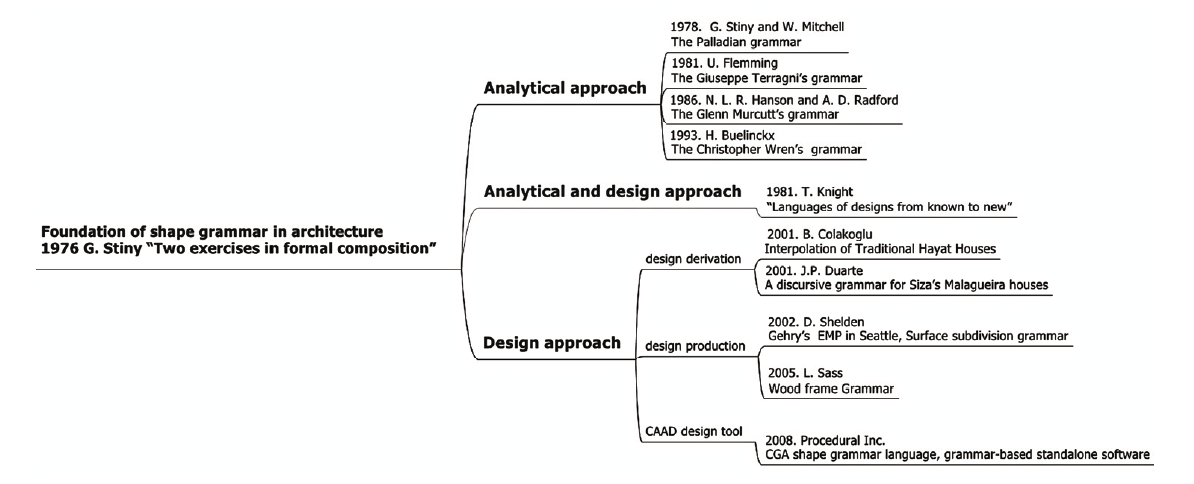
\includegraphics[width=1\textwidth]{shapegrammars.png}
\caption{�rvore Evolutiva das Gram�ticas de Forma } \label{figura:gramaticadeformas}
\end{center}
\end{figure}

A Figura \ref{figura:gramaticadeformas} \cite{tepavcevic2012} mostra uma �rvore evolutiva das GF onde destacam-se as implementa��es capazes de simular "estilos" de arquitetos not�veis (Palladio, Terragni, Siza...). No caso da GF baseada na Casa Malagueira do arquiteto portugu�s �lvaro Siza, \citeonline{duarte2005} relata que o pr�prio autor teve dificuldade de distinguir entre o projeto de sua autoria e algumas das simula��es a ele apresentadas. 

 
\subsection{\textit{L-Systems} (LS)}
\label{subsection:ls}

Os \textit{\textbf{Lindenmayer Systems}}, ou simplesmente \textit{\textbf{L-Systems}}, foram concebidos pelo bot�nico Aristid Lindenmayer como um modelo matem�tico do crescimento de plantas. O conceito inicial, embora n�o tivesse ainda uma representa��o geom�trica, rapidamente evoluiu tornando-se, n�o s� um vers�til modelador de plantas e estruturas org�nicas, como uma ferramenta r�pida para visualiza��o de fractais \cite{prusinkiewicz1996}. Os LS possuem 3 componentes:

\begin{itemize}
\item um conjunto finito de s�mbolos;
\item um conjunto finito de regras de reescrita;
\item uma configura��o inicial dos s�mbolos.
\end{itemize}

Como exemplo podemos ter um conjunto de s�mbolos composto pelas letras "A" e "B", uma configura��o inicial apenas com o s�mbolo "A" e duas regras de escrita:

\begin{itemize}
\item todo s�mbolo "A" deve ser reescrito como "ABA";
\item todo s�mbolo "B" deve ser reescrito como "BBB".
\end{itemize}

Partindo da configura��o inicial e operando por tr�s gera��es geramos:
\begin{center}
A \\
ABA\\
ABABBBABA \\
ABABBBABABBBBBBBBBABABBBABA
\end{center}

Para gerar gr�ficos a partir desta ferramenta basta que se associe formas a cada um dos s�mbolos. Se no exemplo acima o "A" representasse uma linha horizontal ininterrupta e o "B" uma interrup��o na linha, este LS desenharia o fractal "Conjunto de Cantor" (Figura\ref{figura:cantor}).


\begin{figure}[!ht]
\begin{center}
  \mbox{
      \subfigure[Conjunto de Cantor]
         {
            \label{figura:cantor}
            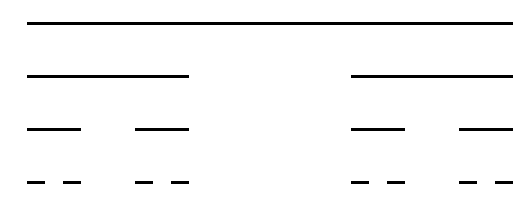
\includegraphics[width=0.40\textwidth]{cantor.png}
         }
  }
  \mbox{
      \subfigure[Curva de Koch - fonte : \citeonline{prusinkiewicz1996}]
         {
            \label{figura:Koch}
            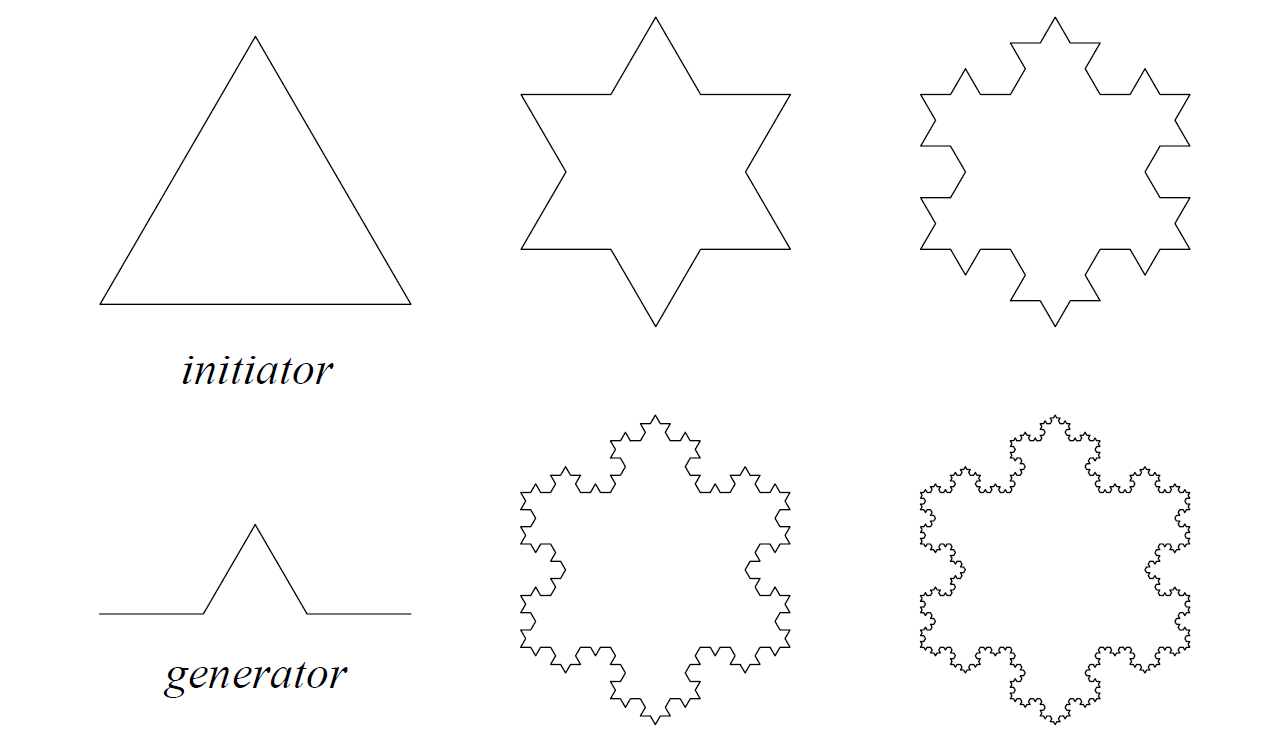
\includegraphics[width=0.50\textwidth]{Koch.png}
         }
  }

\end{center}
\caption{Exemplos de aplica��es dos L-Systems}
\label{figura:LSexemplo}
\end{figure}

Embora os LS sejam definidos como um m�todo de escrita, atrav�s de s�mbolos que representam as formas, uma abordagem gr�fica destes modelos foi tamb�m exposta no livro "The Algorithmic Beaulty of Plants"\cite{prusinkiewicz1996} coescrito pelo autor da proposta original. A Figura \ref{figura:Koch} mostra aa configura��o inicial (\textit{initiator}) onde cada linha do tri�ngulo � substitu�da pelo elemento "\textit{generator}"(que corresponde graficamente � regra de reescrita) na primeira gera��o. O mesmo acontece nas quatro gera��es seguintes, cada linha � redesenhada, mantendo o tamanho e colocando o "\textit{generator}" em escala proporcional ao da linha que este substitui. estas opera��es resultam no fractal conhecido como Curva de Koch.

\begin{figure}[!ht]
\begin{center}
  \mbox{
      \subfigure[Volumetria dos arranha-c�us]
         {
            \label{figura:eVolo072nd0}
            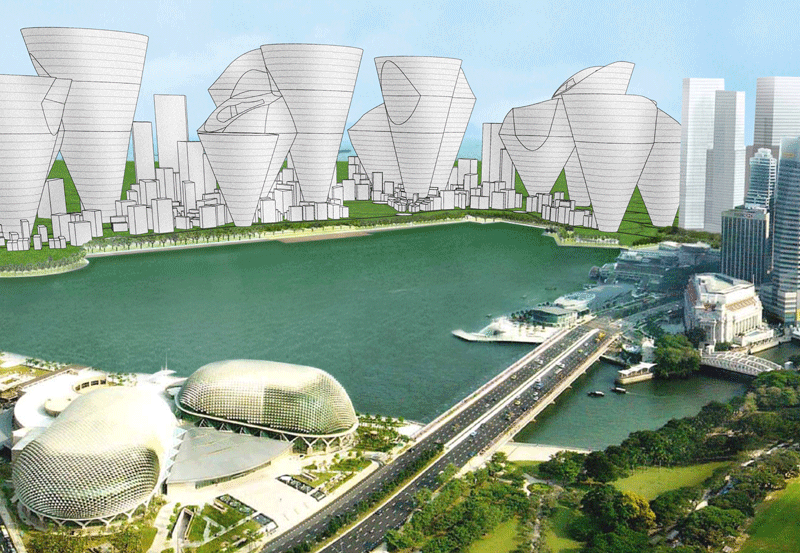
\includegraphics[width=0.30\textwidth]{eVolo072nd0.png}
         }
  }
  \mbox{
      \subfigure[Diagrama estrutural dos arranha-c�us]
         {
            \label{figura:eVolo072nd1}
            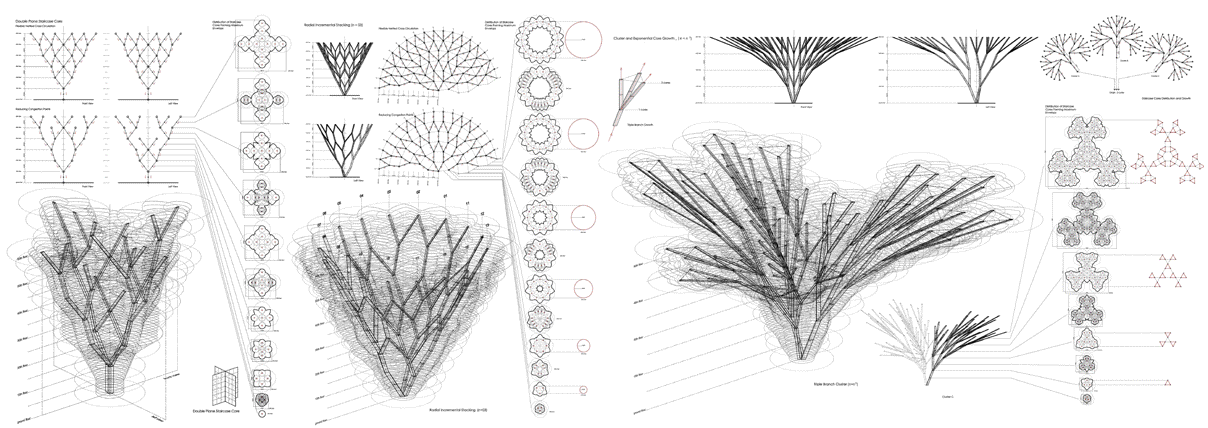
\includegraphics[width=0.60\textwidth]{eVolo072nd1.png}
         }
  }

\end{center}
\caption{Inverted Skyscraper Typology - fonte: \citeonline{inveskytopo}}
\label{figura:LSexemplo1}
\end{figure}


\citeonline{Pascal2006} prop�em uma estrat�gia de modelagem procedural de edif�cios baseado nas Gram�ticas de Chomsky e em L-Systems, objetivando ampla varia��o das formas e grande n�vel de detalhe, aplicado a grandes �reas. \citeonline{daly2009} cita como aplica��o dos LS na Arquitetura a proposta do arquiteto Yi Cheng Pan, premiada com o segundo lugar na edi��o de 2007 do concurso de arranha-c�us promovido pelo peri�dico de Arquitetura eVolo. A ideia consiste na cria��o de grandes edif�cios que ocupem uma �rea diminuta em sua base, liberando o terreno como espa�o p�blico, e que gradativamente, a medida em que se distancia do ch�o, a �rea �til de cada pavimento possa aumentar (Figura \ref{figura:eVolo072nd0}). O diagrama estrutural dos pr�dios, representado na Figura \ref{figura:eVolo072nd1}, baseia-se nas formas encontradas nas ramifica��es dos galhos de �rvores. A aplica��o dos LS se justifica neste caso pela efici�ncia do m�todo na simula��o do crescimento de plantas. 


\subsection{Aut�matos Celulares (AC)}
\label{subsection:autoCel}

Os aut�matos celulares s�o um poderoso e simples modelo matem�tico/computacional com aplica��es importantes em diversas �reas do conhecimento (e.g. F�sica, Biologia, Tecnologia, Artes, Ci�ncias Humanas) \cite{wolfram2002}. A teoria dos aut�matos celulares tem seu in�cio em meados do s�culo XX, nos trabalhos de von Neumann e Morgenstern. O que se buscava era uma formaliza��o matem�tica e l�gica, capaz de contribuir para o entendimento tanto dos sistemas naturais, quanto da computa��o. Podem ser definidos como uma regra evolutiva fixa para um grupo de c�lulas de uma matriz ou grade, onde o tempo � discreto e o estado de cada c�lula e alterado dependendo apenas dos estados anteriores (geralmente apenas o imediatamente anterior), dos seus vizinhos e dela pr�pria \cite{pereira2010}. Posteriormente os fundamentos desta teoria foram estruturados por Wolfram, tendo por base os aut�matos celulares elementares.

Os aut�matos celulares elementares consistem em matrizes unidimensionais onde as c�lulas podem apresentar apenas dois estados ( 0 ou 1, "preto" ou "branco"). O estado de cada c�lula depende apenas do estado anterior dela pr�pria e das vizinhas. Levando em conta que cada c�lula pode apresentar apenas 2 estados, existem oito ($ 2 \times 2 \times 2 $) combina��es poss�veis para o estado de tr�s casas consecutivas. Cada uma destas combina��es determinar� um dos dois valores poss�veis para a c�lula central, o que totaliza 256 regras ($2^8=256$).

\begin{figure}[!ht]
\begin{center}
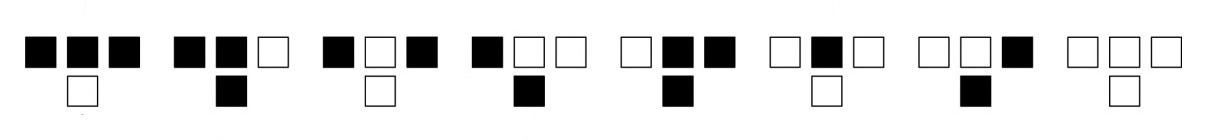
\includegraphics[width=0.80\textwidth]{regra90ac.png}
\caption{Ilustra��o da regra 90 dos AC elementares } \label{figura:regra90ac}
\end{center}
\end{figure}

A Figura \ref{figura:regra90ac} ilustra a regra 90 dos aut�matos celulares elementares. Na linha superior temos as oito combina��es poss�veis, e na linha inferior os resultados de cada combina��a para a regra 90. Na Figura \ref{figura:regra90Sierpinski} cada linha representa uma passagem de tempo onde o valor de cada c�lula � alterado (ou mantido) segundo a regra 90. Partindo de um �nico ponto com o valor "preto", e colocando cada uma das passagens de tempo como se v� na Figura \ref{figura:regra90Sierpinski}, o desenho formado � uma imagem semelhante ao fractal "Triangulo de Sierpinski".

Parindo-se da primeira linha da Figura \ref{figura:regra90Sierpinski}, procura-se determinar qual valor cada uma das c�lulas deve assumir na linha seguinte pela aplica��o da regra descrita na Figura \ref{figura:regra90ac}. O procedimento consiste em, para cada c�lula, considerar o valor dela pr�pria e de suas duas vizinhas imediatas (esquerda e direita), na ordem que elas aparecem na linha (vizinha � esquerda, c�lula a ser reescrita, vizinha � direita). Sempre que as tr�s c�lulas tiverem o valor "branco", aplica-se a oitava posi��o da Figura \ref{figura:regra90ac} e escreve-se "branco" no estado subsequente da c�lula em quest�o. Ao analisar a c�lula imediatamente � esquerda do elemento "preto" central da primeira linha da Figura \ref{figura:regra90Sierpinski}, aplica-se a s�tima posi��o da regra: para a sequ�ncia de valores "branco", "branco", "preto", o estado seguinte da c�lula analisada ser� "preto". Para a c�lula central da primeira linha aplica-se a sexta posi��o da regra 90 e o novo estado da c�lula central � "branco". Para definir o novo estado da c�lula imediatamente � direita do centro aplica-se a quarta posi��o da regra e o valor "preto" � encontrado. As linhas sucessivas da Figura \ref{figura:regra90Sierpinski} s�o determinadas da mesma maneira: observa-se o valor da vizinha � esquerda, da pr�pria c�lula e a da imediatamente � direita, procura-se na regra a mesma sequ�ncia de valores, e utiliza-se o valor de novo estado para essa ordem descrito na regra. 

\begin{figure}[!ht]
\begin{center}
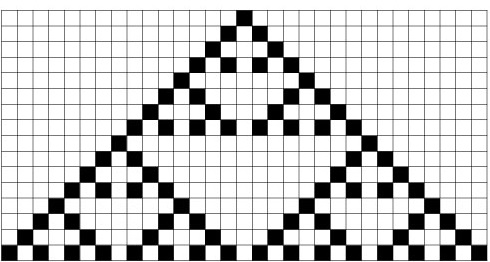
\includegraphics[width=0.60\textwidth]{regra90Sierpinski.png}
\caption{Resultados obtidos a partir de sucessivas aplica��es da regra 90 dos AC elementares - Triangulo de Sierpinski } \label{figura:regra90Sierpinski}
\end{center}
\end{figure}

\citeonline{Herr2007} apresentam uma adapta��o dos AC para proporcionar maior intera��o do projetista com o processo, ao inv�s de deixar o desenho ser unicamente guiado pelas regras de reescrita primariamente definidas. O emprego do AC aparece como um "movimento" opcional de projeto fazendo uso da sua capacidade de gerar variedade formal. Durante o processo � oferecido ao usu�rio a premissa de aceitar as mudan�as propostas pelas regaras e/ou intervir no modelo para direcionar a solu��o do passo seguinte. Um experimento de redesenho de uma proposta para um conjunto de pr�dios proposto para a cidade de Aomori, no norte do Jap�o, pelo grupo de arquitetos espanh�is Cero9 em 2001 (Figura \ref{figura:cero9prop}). Um projeto inspirado em CA onde a inclina��o de cada andar � alterada em fun��o da inclina��o dos andares adjacentes, com os volumes gerados pela adapta��o da mesma proposta com o aux�lio do algoritmo descrito no experimento (Figura \ref{figura:cero9alternativo}) obtendo um jogo volum�trico bastante semelhante.

\begin{figure}[!ht]
\begin{center}
  \mbox{
      \subfigure[Poposta do Grupo Cero9]
         {
            \label{figura:cero9prop}
            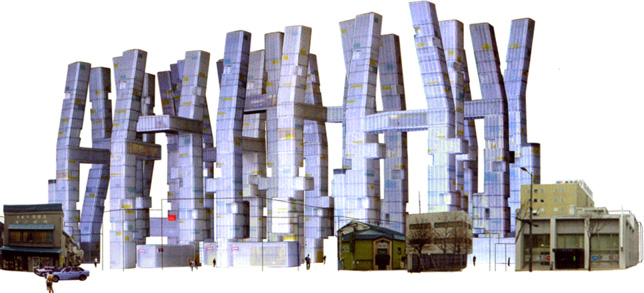
\includegraphics[width=0.40\textwidth]{cero9prop.jpg}
         }
  }
  \mbox{
      \subfigure[Alternativa por Herr e Kvan(2007)]
         {
            \label{figura:cero9alternativo}
            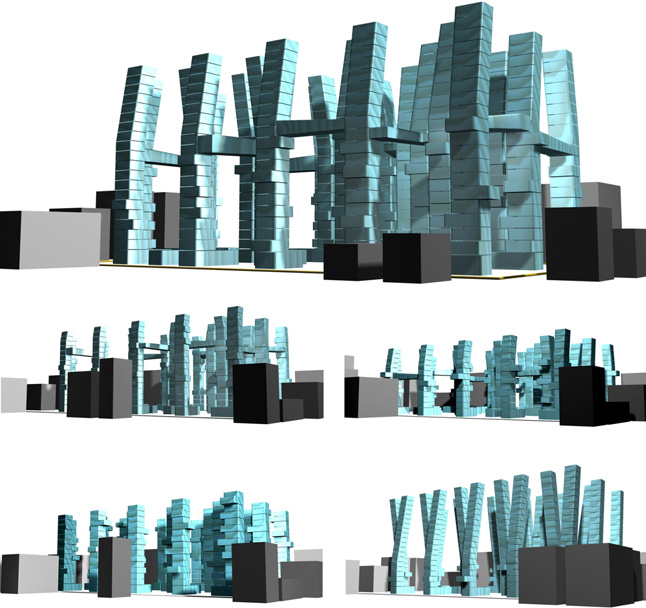
\includegraphics[width=0.50\textwidth]{cero9alternativo.jpg}
         }
  }

\end{center}
\caption{Duas propostas para o conjunto de pr�dios em Aomori/jap�o - fonte: Herr e Kvan(2007)}
\label{figura:Aomori}
\end{figure}


\subsection{\textit{Swarm Intelligence} (SI)}
\label{subsection:si}

\textit{Swarm Intelligence} (intelig�ncia de enxame) � um conjunto de modelos de intelig�ncia artificial baseado no comportamento de coletivos descentralizados e auto-organizados. Lan�ando m�o de Agentes (elementos de programa��o capazes de atuar com autonomia e de acordo com seus pr�prios crit�rios) que interagem, competem e colaboram e assim levam o sistema global ao objetivo almejado \cite{Singh2012}.

Os algoritmos de SI s�o comummente nomeados e classificados em refer�ncia aos seres ou coletivo que os inspirou, entre eles temos:

\begin{itemize}
\item Col�nia de Formigas (\textit{Ant Colony});
\item Col�nia de Abelhas  (\textit{Artificial Bee Colony});
\item Algoritmos das Abelhas (\textit{The Bees Algorithm});
\item Enxame de Part�culas (\textit{Particle Swarm}).
\end{itemize}

As virtudes dos SI nos campos da organiza��o do trabalho, divis�o de tarefas e cronogramas, s�o investigadas tamb�m quando esses campos s�o usados pela Ind�stria da Constru��o Civil. A atividade fim da ICC n�o se passa em um ambiente projetado e planejado como uma planta industrial convencional, mas no terreno escolhido e servido pelo entorno existente (densamente povoado, urbano, rural, etc), o que acarreta em um grade grau de incerteza quanto a qual seria o melhor planejamento para cada caso. \citeonline{Zhang2005} prop�em a aplica��o do modelo baseado em "Enxame de Part�culas" para a defini��o do cronograma de trabalho em atividades de constru��o com limita��es no acesso aos recursos necess�rios. Na mesma linha, porem com um rebatimento formal, \citeonline{Yahya2014} fazem uso de um algoritmo "Col�nia de Abelhas" para o planejamento dos espa�os de um canteiro de obra. Na gera��o de formas a serem constru�das, o trabalho de \citeonline{Luh2011} apresenta um algoritmo para otimiza��o topol�gica de estruturas, baseando-se em um \textit{Particle Swarm} bin�rio. \citeonline[p. 62-71]{aranda2006} discutem estrat�gias de gera��o de formas pela aplica��o de algoritmos inspirados nos coletivos dos p�ssaros (\textit{Flock of Birds}).

\subsection{Diagramas de Voronoi (DV)}
\label{subsection:voronoi}

Definidos de maneira simples e intuitiva: Para um conjunto finito de pontos isolados em um espa�o cont�nuo ($\mathbb{D}^{n}$), associa-se todos os pontos do espa�o ao elemento mais pr�ximo do conjunto de pontos \cite[p. 1]{Okabe2000}. Na Figura \ref{figura:voronoi2d} vemos um DV bi-dimensional com pol�gonos demarcando a regi�o do espa�o em que qualquer dos pontos internos ao per�metro est�o mais pr�ximos do pontos gerador contido no mesmo pol�gono do que de qualquer outro. Os lados do pol�gono ($\mathbb{D}^{n-1}$) est�o equidistante a dois geradores e os v�rtices ($\mathbb{D}^{n-2}$) equidistantes a tr�s pontos. Nos Diagramas 3D, Figura
\ref{figura:voronoi3d}, as faces dos s�lidos ($\mathbb{D}^{n-1}$) representam a regi�o equidistante � dois, as arestas ($\mathbb{D}^{n-2}$) � tr�s e os v�rtices ($\mathbb{D}^{n-3}$) � quatro pontos geradores.

\begin{figure}[!ht]
\begin{center}
  \mbox{
      \subfigure[Diagrama de Voronoi 2D]
         {
            \label{figura:voronoi2d}
            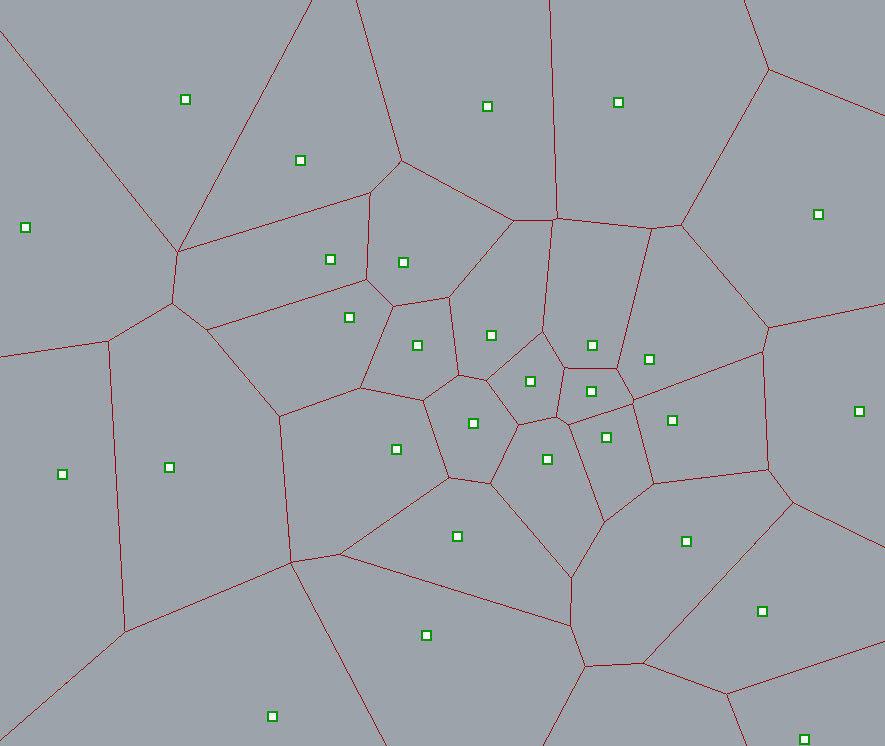
\includegraphics[width=0.45\textwidth]{voronoiRhino.png}
         }
  }
  \mbox{
      \subfigure[Diagrama de Voronoi 3D]
         {
            \label{figura:voronoi3d}
            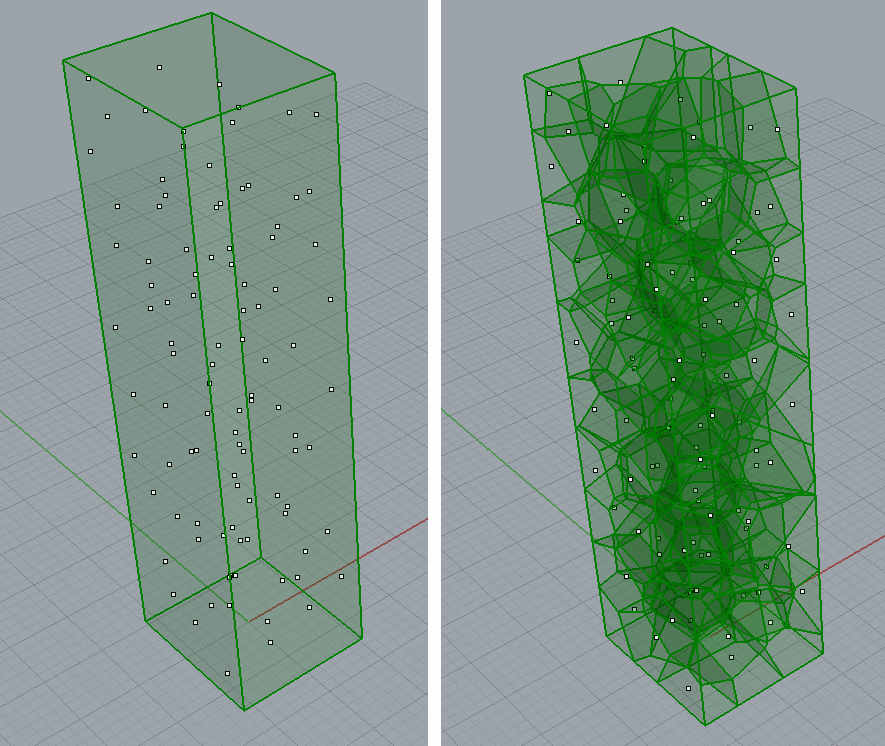
\includegraphics[width=0.45\textwidth]{voronoi3D.png}
         }
  }

\end{center}
\caption{Gerados no \textit{Software \textit{Rhinoceros} 3D}}
\label{figura:voronoi2d-3d}
\end{figure}

A descoberta dos DV (tamb�m chamados de Tesselagem de Dirichlet) � frequentemente atribu�da � Dirichlet (1850) e ao matem�tico Georgy Voronoi (1907) embora tenham sido tratados por Descartes em um estudo sobre a fragmenta��o c�smica, publicado em 1644. Uma estrutura geom�trica vers�til com aplica��es em Geografia, F�sica, Astronomia, Rob�tica, Biologia e muitas outras �reas \cite[p. 147-161]{deberg2008}.

Essas malhas ganharam o interesse de arquitetos pelo seu apelo est�tico org�nico, complexo e, ao mesmo tempo, ordenado. O desenho come�a pela escolha dos pontos geradores do diagrama, o algoritmo desenha a manha do Voronoi, avalia-se o resultado e intervem na disposi��o dos pontos para direcionar o desenho. Sua aplica��o na arquitetura pode ser observada no Centro de Esportes Aqu�ticos da olimp�ada de Pequim (\citeauthor{pwtsite}, Figura \ref{figura:watercube}), onde seu uso busca conferir sensa��o de fluidez ao involucro do pr�dio.

\begin{figure}[!ht]
\begin{center}
  \mbox{
      \subfigure[Centro de Esportes Aqu�ticos - Pequim, China]
         {
            \label{figura:watercube}
            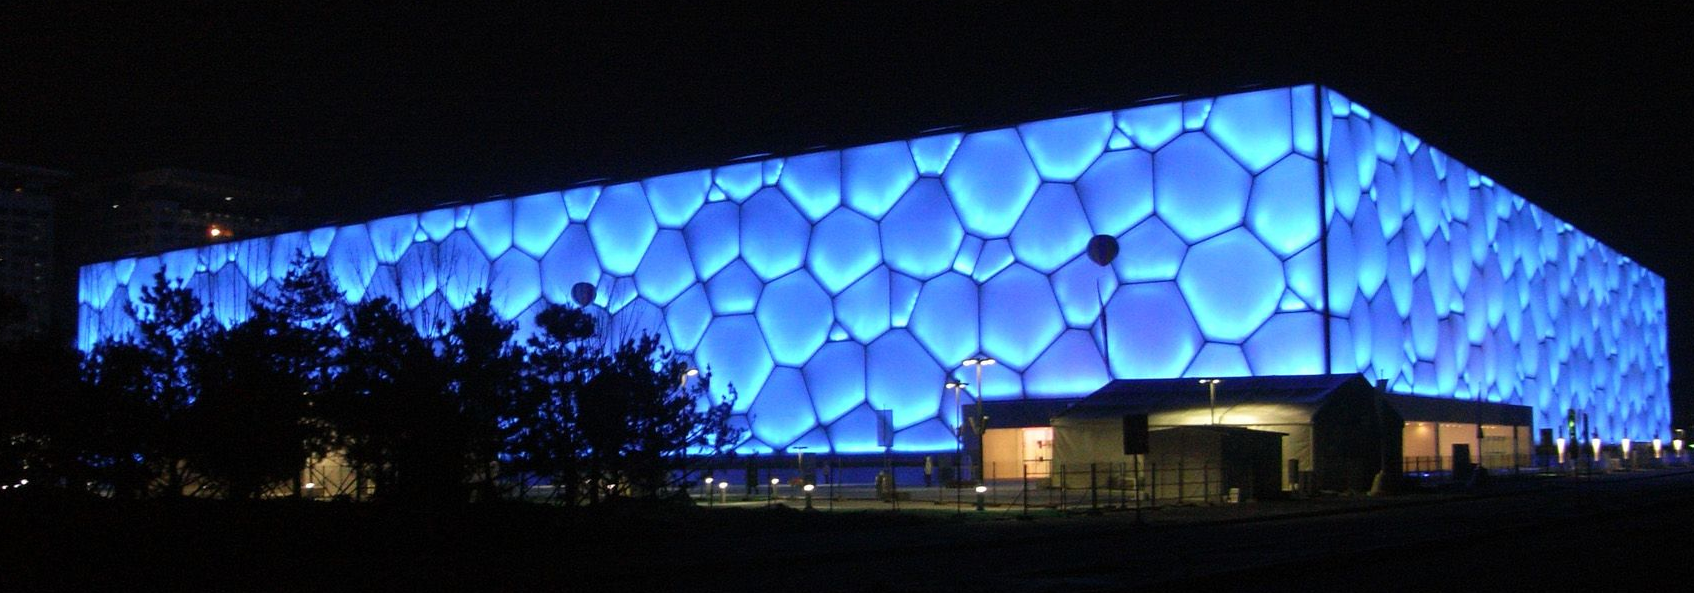
\includegraphics[width=0.55\textwidth]{watercube.png}
         }
  }
  \mbox{
      \subfigure[Jellyfish House]
         {
            \label{figura:Jellyfish_house}
            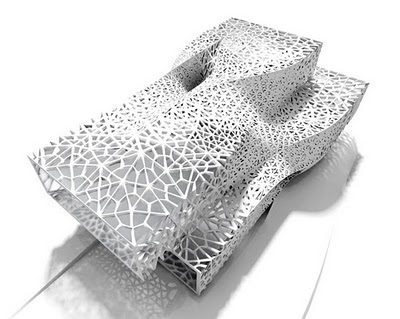
\includegraphics[width=0.35\textwidth]{Jellyfish_house.jpg}
         }
  }


\end{center}
\caption{Exemplos de Diagrmas de Voronoi na Arquitetura}
\label{figura:VoronoiArq}
\end{figure}



O escrit�rio californiano \citeauthor{IwamotoSite} prop�s a \textit{Jellyfish House} (Figura \ref{figura:Jellyfish_house} ) para uma exibi��o de conceitos sobre o futuro pr�ximo das \textit{smart houses}. O fechamento externo apresenta ramifica��es org�nicas, desenhadas com a sobreposi��o de um DV e uma outra malha gerada pela triangula��o de Delauney.


\subsection{Algoritmos de Otimiza��o Estoc�stica}
\label{subsection:algorEstoc}

Tudo que � calculado ou representado em computa��o; a altura de um pr�dio, O raio de um circulo, a inclina��o de um telhado, a largura de uma rua, o calor do sol, a velocidade do vento, etc; � feito atrav�s de vari�veis. A otimiza��o � a procura dos valores ideais de vari�veis, para que o cen�rio descrito por elas possa ser configurado da melhor maneira poss�vel. Quando o problema � simples e bem definido (e.g. qual a menor quantidade em $m^2$ de paredes e laje de uma caixa-d'�gua para armazenar 5.000 litros de �gua?), os m�todos determin�sticos s�o suficientes para se encontrar com exatid�o o resultado ideal. Quando o n�mero de vari�veis � grande e/ou a fun��o que relaciona estas � grandeza que se pretende otimizar � muito complexa ou o que se entende por "melhor cen�rio poss�vel" n�o � muito bem determinado, a otimiza��o determin�stica n�o � suficiente para solucionar o problema e outros modelos ganham import�ncia.
 
A otimiza��o estoc�stica refere-se aos m�todos de procura por uma solu��o ideal (em rela��o a um objetivo determinado) onde a aleatoriedade est� envolvida de forma construtiva. Os principais algoritmos de otimiza��o estoc�stica s�o \cite{Fouskakis2002}:

\begin{itemize}
\item Algoritmos Gen�ticos
\item \textit{Simulated Annealing} 
\item \textit{Tabu Search}
\end{itemize}

\subsubsection{Algoritmos Gen�ticos}
\label{subsection:algorEstocAG}

Os Algoritmos Gen�ticos s�o, dentre os m�todos de otimiza��o estoc�sticos, os mais aplicados na Arquitetura \cite{Singh2012}. Propostos por John Holland em 1975 \cite{Lodding2004}, estes algoritmos s�o modelos computacionais inspirados nos conceitos darwinianos de sobreviv�ncia dos mais aptos \cite{Caldas2002}. Opera��es de sele��o e recombina��es s�o aplicadas entre as solu��es candidatas na procura dos que apresentam um melhor desempenho. A terminologia usada tamb�m faz analogia com a teoria da evolu��o das esp�cies: as solu��es candidatas s�o chamadas de indiv�duos, os grupos de indiv�duos existentes em cada estado � denominado de popula��o, cada vez que uma nova popula��o � criada, chama-se de gera��o. As principais opera��es realizados por um algoritmo gen�tico s�o: a reprodu��o, o \textit{crossover} e a muta��o.

\begin{figure}[!ht]
\begin{center}
  \mbox{
      \subfigure[\textit{Integrated Design} - \citeonline{fasoulaki2008}]
         {
            \label{figura:integated_design}
            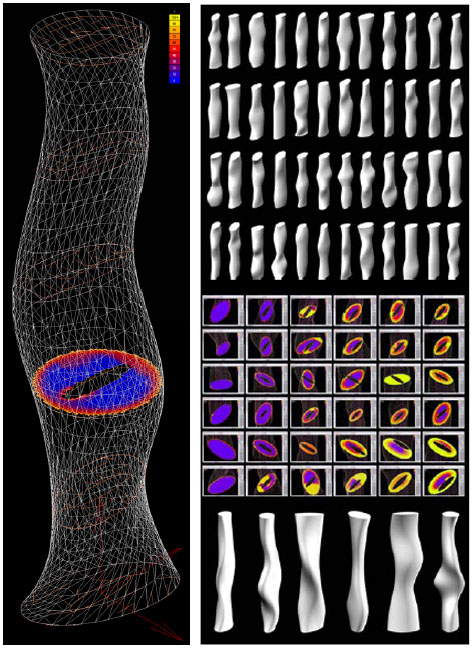
\includegraphics[width=0.30\textwidth]{integated_design.jpg}
         }
         
         \quad
         \quad

        \subfigure[Fachadas Escolhidas, Gene Arch - \citeonline{Caldas2008} ]
           {
              \label{figura:GeneArch}
              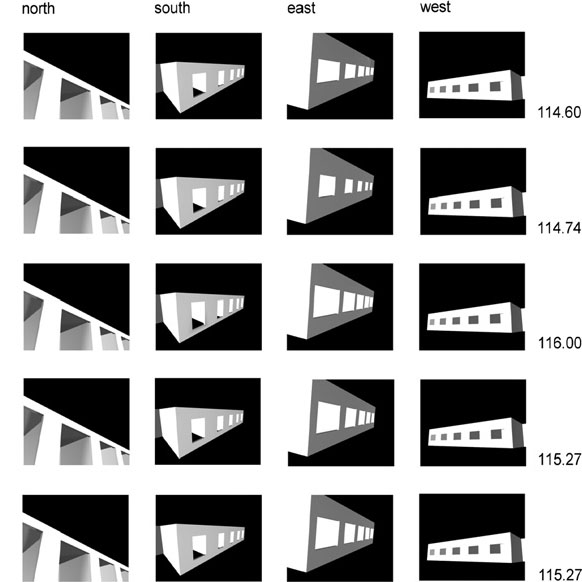
\includegraphics[width=0.42\textwidth]{GeneArch.jpg}
           }
    }

\end{center}
\caption{Exemplo de Aplica��es de Algoritmos Gen�ticos na Arquitetura}
\label{figura:geneticos}
\end{figure}

Inicialmente o algoritmo gera aleatoriamente uma popula��o inicial de indiv�duos, um conjunto de poss�veis configura��es das vari�veis do problema. Em seguida aplica-se a fun��o objetivo, tamb�m chamada de \textit{fitness function} ou fun��o de aptid�o, para todos os candidatos gerados no passo anterior. A \textit{fitness function} alude ao conceito evolucionista em que os mais aptos sobrevivem. Na s�rie de trabalhos desenvolvidos por \citeonline{caldas1999}, (\citeyear{cladas2001}), (\citeyear{Caldas2002}),  (\citeyear{Caldas2008}) o que se pretende analisar � a temperatura e ilumina��o resultante das dimens�es das janelas de fachadas com orienta��es distintas, em diferentes cidades do mundo. Os indiv�duos s�o configura��es das fachadas com variadas dimens�es de abertura para  cada fachada. A \textit{fitness function} se alimenta pelos valores de  ilumina��o e temperatura analisada pelo software DOE2.1E. Simulando as caracter�sticas clim�ticas de uma cidade espec�fica, o \textit{software} recebe os par�metros de cada individuo e calcula a sensa��o t�rmica e a ilumina��o em um c�modo com essas configura��es e a energia gasta para que, com ilumina��o e controle t�rmico artificiais, o ambiente se aproxime de condi��es definidas como ideais. A partir desses dados, ordenam-se os indiv�duos de acordo com a efici�ncia energ�tica de cada an�lise, medindo-se assim a aptid�o � "sobreviv�ncia" de cada candidato. As melhores solu��es s�o eleitas para a pr�xima fase. O \textit{crossover} permite reorganizar partes de duas solu��es eleitas, gerando uma nova configura��o, um novo individuo integrante de uma nova gera��o e muta��es ocorrem com definida probabilidade sobre os indiv�duos da popula��o. Os trabalhos evoluem e um \textit{software} de otimiza��o baseado em algoritmos gen�ticos para Arquitetura, o \textit{Gene Arch}, � apresentado \ref{figura:GeneArch}.

Muta��o � um evento aleat�rio que ocorre com uma probabilidade definida pelo usu�rio para alguns indiv�duos da popula��o. � aplicada para garantir a diversidade gen�tica da nova gera��o \cite{fasoulaki2005}\footnote{\textit{Mutation is a random event, occurring with a user-defined probability to only some of the new offspring. It is used to maintain genetic diversity by altering only a little piece of the new offspring.}}. As opera��es s�o repetidas seguidamente, de gera��o � gera��o, analisando candidatos at� que os crit�rios de parada do algoritmo sejam atendidos e a solu��o otimizada seja escolhida.

No experimento proposto por \citeonline{fasoulaki2008} quatro caracter�sticas de um edif�cio em Nova York s�o otimizadas: o insolejamento, a estrutura, a ventila��o e maximiza��o da �rea constru�da de acordo com as limita��es do c�digo de obras da cidade. O modelo � parametrizado em sete pavimentos de controle el�pticos igualmente distantes. Neles O desempenho t�rmico e a ilumina��o s�o avaliados. A volumetria � criada a partir da interpola��o de uma superf�cie entre as linhas de contorno de cada pavimento de controle. A �rea das interse��es de planos na altura de cada andar (para este c�lculo n�o s�o utilizados apenas os pavimentos de controle) � somada para se aferir o valor da �rea constru�da . Avalia-se atrav�s de uma planilha o custo estimado da estrutura de cada candidato. Os genes controlam a posi��o e rota��o de cada pavimento de controle e as muta��es transformam pavimentos el�pticos em circulares. A fun��o de aptid�o � avaliada ap�s normalizarem-se os valores de cada an�lise entre zero e um, atribuindo-se pesos para cada uma das quatro caracter�sticas estudadas. O m�todo, intitulado \textit{Integrated Design} (Figura )\ref{figura:integated_design}), defende uma negocia��o entre os diversos profissionais envolvidos no projeto, ouvindo especialistas de cada �rea para que se definam os pesos. A grosso modo, � a tentativa de estabelecer uma propor��o entre o benef�cio de uma melhor insola��o com o custo estrutural que isso acarreta, por exemplo.


\subsubsection{\textit{Simulated Annealing} (SA)}
\label{subsection:algorEstocSA}

Supondo que, em um problema de otimiza��o onde se procura o valor m�nimo de uma fun��o utilize-se o seguinte m�todo: uma configura��o inicial, representada pelo ponto $P1$ � fornecida para o problema. Outros pontos s�o escolhidas aleatoriamente na vizinhan�a do $P1$, chamados aqui genericamente de $Pn$. A fun��o objetivo $F(x)$ � avaliada para os novos pontos. Caso o valor da fun��o objetivo para $Pn$ seja menor que o valor da fun��o objetivo em $P1$, a configura��o $Pn$ � armazenada como um candidato poss�vel para melhor solu��o. Se $F(P1)<F(Pn)$, o ponto $Pn$ � descartado.


\begin{figure}[!ht]
\begin{center}
  \mbox{
      \subfigure[\textit{Hill Climbing}]
         {
            \label{figura:hillclimbing}
            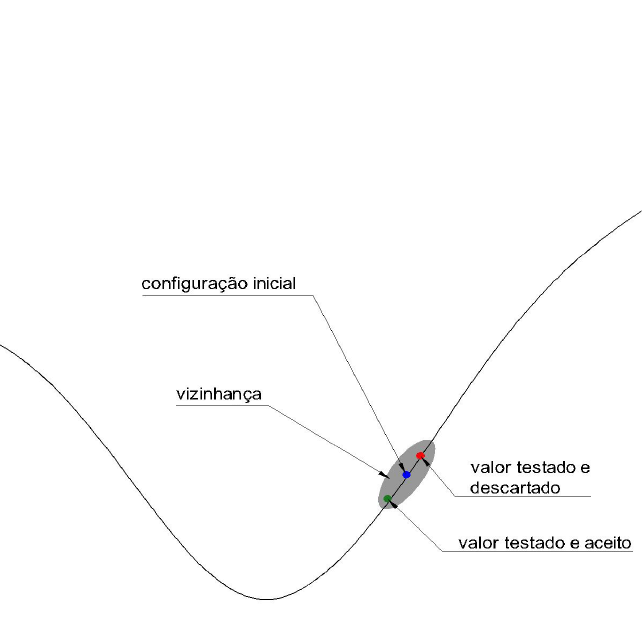
\includegraphics[width=0.45\textwidth]{hillclimbing.png}
         }
         
         
         

        \subfigure[M�nimo Local e Gobal]
           {
              \label{figura:MINIMO_LOCAL}
              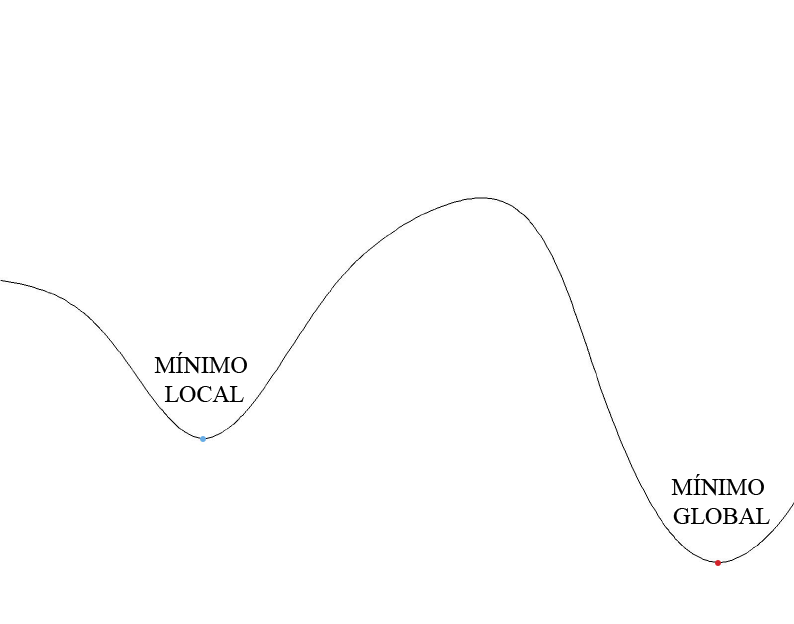
\includegraphics[width=0.45\textwidth]{MINIMO_LOCAL.png}
           }
         }
         
  \mbox{
           \subfigure[Curva Exponencial]
                      {
                         \label{figura:exponencial}
                         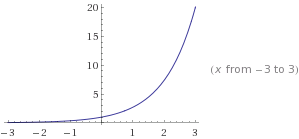
\includegraphics[width=0.45\textwidth]{exponencial.png}
                      }
                      
                      
           \subfigure[\textit{Simulated Annealing}]
                                 {
                                    \label{figura:SA_conceito}
                                    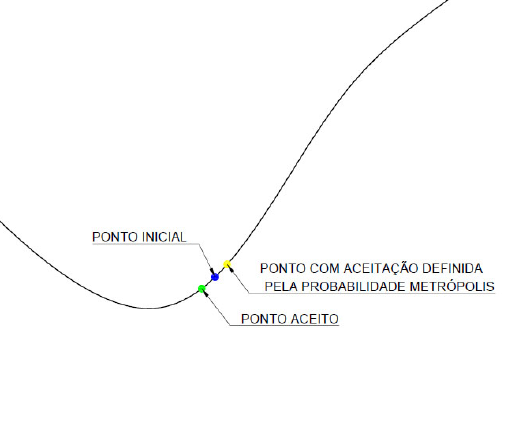
\includegraphics[width=0.45\textwidth]{SA_conceito.png}
                                 }
    }
 

\end{center}
\caption{\textit{Simulated Annealing} - Conceitua��o}
\label{figura:baseSA}
\end{figure}

O m�todo descrito acima se chama \textit{hill climbing}, ilustrado na Figura \ref{figura:hillclimbing}. Apresenta grande velocidade de converg�ncia, caso o problma seja bem definido, a fun��o objetivo seja simples ou o ponto inicial seja convenientemente escolhido. Em casos onde a fun��o apresenta uma curva menos previs�vel, apresentando m�nimos locais e um m�nimo global, como no exemplo da Figura \ref{figura:MINIMO_LOCAL}, dependendo do ponto inicial escolhido, o procedimento apresentado pode convergir para um m�nimo local e ficar estacionado. Em fun��es objetivos complexas e com n�mero de vari�veis maior que dois, a determina��o da regi�o que faria o resultado do \textit{hill climbing} convergir para o m�nimo global costuma ser impreciso.

O \textit{Simulated Annealing}, ou recosimento simulado, prop�e uma altera��o no algoritmo \textit{hill climbing} baseando-se no processo metal�rgico do recosimento (\textit{annealing}) e no algoritmo Metropolis-Hastings. O objetivo desta implementa��o � um m�todo de otimiza��o que consiga executar uma varredura mais completa no espa�o de solu��es do problema, evitando que o resultado fique sujeito � converg�ncia em m�nimos locais.

O recosimento � um processo metal�rgico de se resfriar gradualmente um corpo, com uma queda lenta e controlada da temperatura para que as mol�culas formem cristais, a acomoda��o que acarreta em uma menor energia para o sistema. Caso a queda da temperatura seja brusca, a tend�ncia � vitrificar, equivalendo a m�nimos locais no que diz respeito � minimiza��o da energia do sistema.

O algoritmo Met�polis-Hastings, ou simplesmente o algoritmo Metr�polis, se encaixa perfeitamente na analogia criada por se tratar de uma aplica��o do algoritmo probabil�stico de Monte-Carlo para simular a configura��o energ�tica mais prov�vel das mol�culas de um sistema em equil�brio t�rmico. O modelo f�sico utilizado para relacionar energia com temperatura foi a distribui��o de Boltzmann, descrita na equa��o \ref{equacao:sa}:


\begin{equation}
\label{equacao:sa}
P(E)= e^{x}
\verb| , sendo |
x=\frac{-\Delta E}{k \times T}
\end{equation}



A distribui��o de Boltzmann parte da no��o F�sica de que as part�culas de um sistema em equil�brio t�rmico n�o tem todas a merma energia. A distribui��o desta energia n�o acontece por igual, de forma que a soma de pequenas partes iguais resultem na temperatura do sistema. Calcula-se aqui a probabilidade, $P()$, de uma dessas mol�culas ter determinada energia, $E$, em fun��o da varia��o da energia global, $\Delta E$, e da temperatura do sistema, $T$. O $k$ � a chamada constante de Boltzmann ($1,38 \times 10\mathbb{}^{-23} J/K$), e a curva da probabilidade, $P(E)$ apresenta a forma de uma exponencial, $e^{x}$, mostrada na Figura \ref{figura:exponencial}. 

Os algoritmos SA possuem tr�s requisitos b�sicos:

\begin{itemize}
\item uma fun��o objetivo;
\item uma configura��o inicial das vari�veis;
\item uma agenda de resfriamento.
\end{itemize}

Semelhante ao modelo \textit{Hill Climbing}, configura��es aleat�rias s�o escolhidas na vizinhan�a da configura��o inicial. Caso o valor da fun��o objetivo seja menor em um ponto sorteado na vizinhan�a do que na configura��o inicial, esse ponto � aceito no conjunto das configura��es, caso contrario, o ponto n�o � imediatamente descartado como no \textit{Hill Climbing}, mas se aceita ou refuta o candidato de acordo com uma probabilidade baseada na distribui��o de Boltzmann (Figura \ref{figura:SA_conceito} ).

Para os pontos com fun��o objetivo maior que � inicial, a probabilidade de ingresso no conjunto de candidatos aceitos � definida por uma avalia��o da fun��o $P(E)$, tendo por $\Delta E$ a varia��o da fun��o objetivo para $P(1)$ e $P(n)$ e $T$ a temperatura atual da agenda de resfriamento. A temperatura tem import�ncia determinante no valor da probabilidade e perman�ncia do novo ponto. Se $T$ tem um valor muito alto, $x$ ser� um valor negativo muito baixo, levando a fun��o $e^x$ assumir posi��o pr�xima a 1 no gr�fico da Figura \ref{figura:exponencial}. a medida que $T$ diminui, o valor de $e^x$ se aproxima de zero. Com a probabilidade calculada, um n�mero entre zero e 1 � sorteado (algoritmo pseudo-rand�mico). Se a probabilidade � maior que o n�mero sorteado, o ponto � aceito, caso contrario � descartado. E o processo reinicia tendo os membros do conjunto dos candidatos aceitos como configura��o inicial.

A agenda de resfriamento define de quantos em quantos \textit{loops} a temperatura sera controladamente reduzida, e quais valores vai assumir ao longo do tempo de execu��o do SA. Os crit�rios s�o definidos pelo usu�rio � podem variar de acordo com o problema a ser otimizado.

No in�cio de sua execu��o, a probabilidade de aceita��o de valores rejeitados pelo \textit{Hill Climbing} � muito grande, permitindo ao SA explorar amplamente o espa�o de solu��es poss�veis. Com o resfriamento simulado no algoritmo, menos candidatos com $P(1)<P(n)$ s�o aceitos e os candidatos tendem a convergir para diversos m�nimos locais, eventualmente encontrando o m�nimo global do sistema \cite{Kirkpatrick1983}.

\citeonline{Lamberti2008} prop�e uma varia��o do SA denominada CLMPSA (\textit{Corrected Multi-Level Multi-Point Simulated Annealing}), descrevendo detalhadamente a estrutura do algoritmo para a otimiza��o estrutural de treli�as. O m�todo procura mover configura��es de maior valor para a fun��o objetivo antes de fazer o teste probabil�stico, mostra um crit�rio de defini��o da agenda de resfriamento em fun��o das varia��es da energia do sistema e compara os resultados com implementa��es do SA alternativas e outros m�todos de otimiza��o. \citeonline{Sonmez2007} usa o SA para otimiza��o de forma estrutural submetida a carregamento quasi-est�tico representada em duas dimens�es.


%\subsubsection{\textit{Tabu Search}}
%\label{subsection:algorEstocTS}


\subsection{Fractais}
\label{subsection:fractais}

Embora n�o seja exatamente um algoritmo, mas possam ser gerados por uma gama destes, os fractais s�o uma das mais importantes descobertas  cientificas do s�culo XX. Uma particularidade interessante � que estas formas geom�tricas atra�ram a aten��o n�o s� de cientistas, mas tamb�m de artista e \textit{designers}. Na Arquitetura n�o foi diferente. O escrit�rio \citeonline{hparc}, por exemplo, no projeto do \textit{Grand Egyptian Museum} em Giz� no Egito, utiliza do Tri�ngulo de Sierpinski em uma fachada lateral transl�cida tanto como uma alus�o � emblem�tica imagem hist�rica das pir�mides quanto como um contraponto est�tico contempor�neo.

\begin{figure}[!ht]
\begin{center}
  \mbox{
      \subfigure[\textit{Grand Egyptian Museum} Giz�, Egito - fonte: \citeonline{hparc}]
         {\label{figura:grandEgyptianmuseum}
          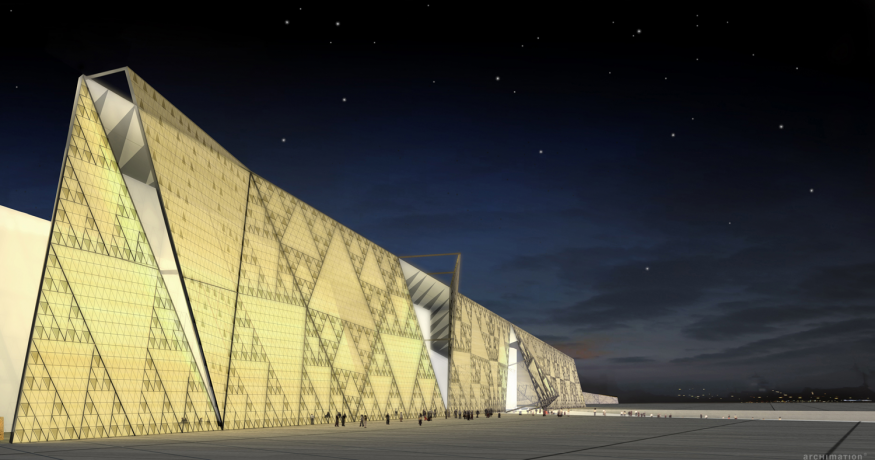
\includegraphics[width=0.71\textwidth]{grandEgyptianmuseum.png}
         }
         
         
        \subfigure[\textit{Federation Square of Melbourne} - fonte: \citeonline{Hammer2006} ]
           {\label{figura:fsm}
            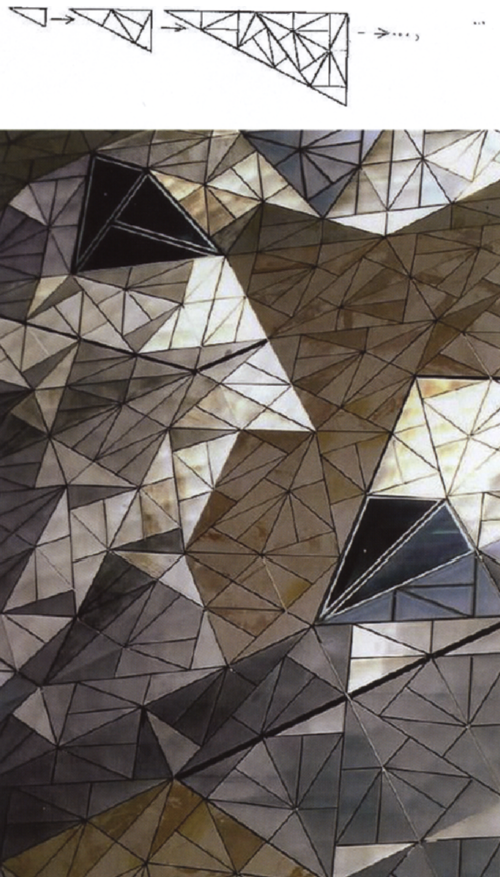
\includegraphics[width=0.21\textwidth]{FederationSquare.png}
           }
       }

\end{center}
\caption{Exemplos de Utiliza��o dos Fractais na Arquitetura}
\label{figura:fractaisArqExemplos}
\end{figure}



O termo fractal foi cunhado pelo matem�tico Benoit Mandelbrot em um artigo publicado em 1975. Tem por raiz a palavra \textit{fractus}, oriunda do latim, significando "quebrado" ou "fragmentado". Aplicando processos de computa��o gr�fica para estudar o comportamento de m�todos iterativos na resolu��o de certas equa��es complexas (tendo por base alguns trabalhos do matem�tico Gast�n Julia), gerou-se  uma s�rie de gr�ficos onde propriedades geom�tricas divergentes das estabelecidas nos estudos euclidianos foram encontradas, estudadas e mesuradas. Ao ramo da Matem�tica que trata dos elementos que possuem estas propriedades foi dado o nome de Geometria Fractal.  O livro "The Fractal Geometry of Nature" de Benoit Mandelbrot \cite{mandelbrot1983fractal} que, segundo o pref�cio do autor, � uma extens�o e corre��o de seus artigos anteriores sobre o tema; parte da ideia de que uma montanha n�o � um cone e as nuvens n�o s�o esferas, propondo uma abordagem cient�fica aplic�vel ao estudo de formas n�o euclidianas. Como principais caracter�sticas dos fractais est�o a auto-similaridade (ligada ao conceito de escala),  replicabilidade infinita e  a dimens�o de Hausdorff diferente da dimens�o euclidiana (muitas vezes n�o sendo um n�mero inteiro).

Para facilitar a apreens�o dos conceitos b�sicos, tomou-se como exemplo o fractal proposto pelo matem�tico polon�s Waclaw Franciszek Sierpinski em 1915, o Tri�ngulo de Sierpinski. Embora a figura proposta seja anterior � cria��o deste ramo da geometria, n�o esta s� entre as constru��es matem�ticas preexistentes que se encaixam no conceito.

Sua constru��o se d� pelo desenho inicial de um triangulo, a partir do qual um segundo triangulo � formado pela liga��o dos pontos m�dios dos lados do primeiro. Considera-se que este segundo tri�ngulo � uma subtra��o da �rea do original (quebra ou fragmenta��o). Tem-se agora tr�s tri�ngulos e um vazio triangular(Figura \ref{figura:sierpinskigrasshopper2D}). Em cada um dos tri�ngulos o procedimento � refeito, gerando mais tr�s tri�ngulos para cada. Repete-se a opera��o infinitas vezes e a cada etapa se d� o nome de itera��o, numerando-as a partir da primeira vez que a forma inicial � subdividida (primeira itera��o).

\begin{figure}[!ht]
\begin{center}
  \mbox{
      \subfigure[Tri�ngulo de Sierpinski 2D]
         {
            \label{figura:sierpinskigrasshopper2D}
            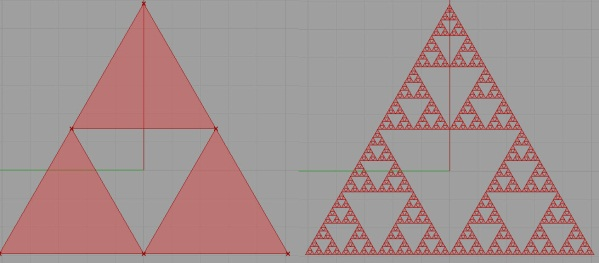
\includegraphics[width=0.45\textwidth]{sierpinskigrasshopper.png}
         }
  }
  \mbox{
      \subfigure[An�logo 3D do Tri�ngulo de Sierpinski]
         {
            \label{figura:sierpinskigrasshopper3D}
            \includegraphics[width=0.45\textwidth]{sierpinskigrasshopper3d.png}
         }
  }

\end{center}
\caption{Gerados no \textit{Rhino3d/Grasshopper} utilizando o \textit{add-on Hoopsnake} para uma e cinco itera��es}
\label{figura:sierpinskigrasshopper}
\end{figure}


A partir da Figura \ref{figura:sierpinskigrasshopper}, gerada no ambiente \textit{Rinoceros / Grasshopper} (ver Ap�ndice \ref{Apend2:triSierp}) pode-se aferir pela simples observa��o duas das caracter�sticas b�sicas dos fractais e calcular a terceira. Nota-se que pequenos peda�os do desenho reproduzem o todo. Tendo em mente a ideia de uma constante aproxima��o da figura, de tal forma que a escala dos tri�ngulos menores vai aumentando e, em dado momento, um deles assume o tamanho do triangulo inicial. � intuitivo perceber que a imagem encontrada � semelhante ou mesmo igual (caso n�o se possa enxergar qualquer peda�o contido nos outros tri�ngulos gerados na mesma itera��o, e o n�mero de itera��es seja equivalente para se ter o mesmo n�vel de detalheda imagem) � figura como era vista antes da aproxima��o. A capacidade dos fractais de carregar em suas partes a representa��o do todo se d� o nome de auto-similaridade.

\begin{figure}[!ht]
\begin{center}
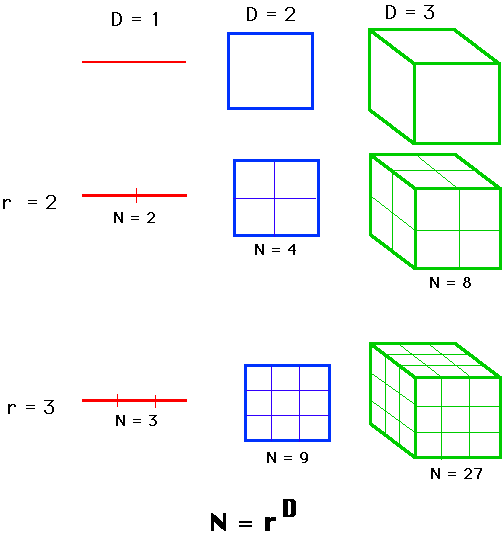
\includegraphics[width=0.50\textwidth]{haussdorf.png}
\caption{Dimens�o de Haussdorf - fonte: http://en.wikipedia.org/wiki/Fractal\_dimension} \label{figura:haussdorf}
\end{center}
\end{figure}

Um dos interesses cient�ficos  no estudo dos Fractais � a sua ocorr�ncia na natureza. Uma planta onde suas estruturas ramificam-se  repetindo em escala reduzida formas semelhantes ao todo (ou a parte do todo) � o que se observa no tri�ngulo de Sierpinski sob o conceito de auto-similaridade (uma parte representa o todo). A replicabilidade infinita, a possibilidade de observar elementos recorrentes independentemente de quantas (infinitas) aproxima��es (itera��es) sejam efetuadas, s� � encontrada em fractais da Matem�tica. O racioc�nio que embasa o c�lculo da dimens�o fractal, tamb�m chamada de dimens�o de Haussdorf,  � ilustrado na Figura  \ref{figura:haussdorf}. Para cada uma das dimens�es cartesianas desenhou-se uma figura que a representasse (uma reta, um quadrado e um cubo).  Cada uma das dimens�es  de cada figura � dividida em um n�mero qualquer (porem igual para cada dimens�o) de vezes.

Sendo $r$ o n�mero de subdivis�es em cada dimens�o e $N$ o n�mero de figuras semelhantes � inicial geradas por $r$ subdivis�es, tem-se $N=r^{D}$, onde $D$ � a dimens�o euclidiana da figura. A vari�vel $r$ pode tamb�m ser escrita como $L/u$, onde $L$ � o tamanho de cada dimens�o da figura e $u$ o tamanho de cada subdivis�o. Coloca-se $D$ em evid�ncia encontra-se a equa��o \ref{equacao:haussdorf}.

\begin{equation}
\label{equacao:haussdorf}
D= \frac{\log{N}}{ \log{L/u}}
\end{equation}

 
Para todas as formas e divis�es mostradas na Figura \ref{figura:haussdorf} o valor $D$ calculado ser� igual ao n�mero de dimens�es euclidianas que cada geometria representa (um para a reta, dois para o quadrado, tr�s para o cubo). Aplicando a equa��o \ref{equacao:haussdorf} para calcular a dimens�o fractal do Tri�ngulo de Sierpinski, onde cada lado $L$ � dividido duas vezes por itera��o, $L/u=2$, formando tr�s figuras semelhantes a inicial, $N=3$. Logo $D=\frac{\log{3}}{\log{2}}$. Portanto a dimens�o de Haussdorf do fractal � de $1,5849$.

Mas os n�meros n�o importam por enquanto. Em um n�vel mais profundo do estudo, esses n�meros traduzem informa��es sobre a natureza das coisas. Primeiramente � recomend�vel entender o significado do que eles medem: a maneira como o espa�o se dobra, a quantidade da rugosidade de uma superf�cie, a textura das formas da natureza, as curvas da linha entre a praia e o mar, o detalhe de como certos tipos de mat�ria se agrega. Imagens direta ou indiretamente presentes nos pensamentos sobre a constru��o. A dimens�o fractal � uma quantidade num�rica que aproxima as ramifica��es dos galhos da �rvore � seu todo.

Em 1997 o escrit�rio de arquitetura londrino \textit{Lab Architectural Studio} ganhou o concurso internacional para o projeto de um centro cultural, o \textit{Federation Square} na cidade de Melbourne, Austr�lia. A Figura \ref{figura:fsm} mostra um detalhe da fachada de um tr�s pr�dios principais do conjunto (abaixo) e a estrat�gia utilizada na subdivis�o dos tri�ngulos sucessivamente em cinco tri�ngulos menores (acima), mantendo sempre a propor��o de 1:2 entre os lados perpendiculares. Os tri�ngulos s�o constru�dos de tr�s materiais: vidro, arenito e zinco. Um mosaico multifacetado e multicolorido, segmentando, absorvendo, refletindo e enquadrando a luz e definindo os espa�os de forma peculiar e fragmentada \cite{Hammer2006}.


\subsection{Modelos de Par�metros e Restri��es (MPR)}
\label{subsection:agParam}

Todos os algoritmos generativos, bem como toda computa��o, baseiam-se em par�metros. Os modelos param�tricos, contudo se diferenciam dos demais por colocar a �nfase na manipula��es destes \cite{DIno2012}. A modelagem param�trica permite altera��o a qualquer momento de algumas vari�veis e o autom�tico rebatimento desta altera��o no modelo. Desenhando um prisma quadrangular reto (paralelep�pedo), deve-se fornecer valores reais para a altura, largura e profundidade. Na modelagem param�rica � permitido alterar qualquer uma dessas vari�veis, redesenhado o prisma automaticamente.

Os modelos param�tricos de projeto pode ser divididos em dois tipos: conceituais e construtivos. Os �ltimos tem por principais par�metros as informa��es envelopadas em formas 3D predeterminadas. Esses modelos desempenham papel crucial na implementa��o do conceito de BIM, visto que seu objetivo � agregar o maior n�mero de informa��es construtivas poss�veis dentre os seus par�metros. Nos modelos conceituais os par�metros de projeto s�o definidos em primeira etapa e guiam a procura pela forma. Representando uma mudan�a mais radical no processo de projetar que os modelos param�tricos construtivos \cite{Milena2010a}. Essa mudan�a no processo coloca os modelos param�tricos conceituais dentro do campo de estudo dos Algoritmos Generativos. 

As duas categorias, porem n�o s�o estanques. \citeonline{Donath2009}, por exemplo, desenvolvem um modelo param�trico conceitual para projeto da forma externa de pr�dios residenciais isolados e de grande altura que, desde a instiga��o inicial, apoia-se em uma ferramenta especializada em modelos param�tricos construtivos, tornando evidente a facilidade com que as informa��es construtivas poder�o ser inseridas durante o processo.

Dentre as principais qualidades de um Modelo Param�trico est� a capacidade de resolver quest�es bem definidas, com um objetivo claramente descrito, quando de abordar quest�es pouco definidas e complexas que apresentam diversas solu��es vi�veis \cite{DIno2012}.

Os Modelos Param�tricos Conceituais s�o aqui tratados como Modelos de Par�metros e Restri��es por raz�es t�cnicas e metodol�gicas. A ideia � enfatizar na nomenclatura a import�ncia tanto dos par�metros quanto das regras implementadas na forma de algoritmos, que geram as formas geom�tricas � serem estudadas. Essas regras, falando especificamente da Modelagem Param�trica Conceitual, podem ser entendidas como restri��es. Esta abordagem mostrou-se eficiente, do ponto de vista metodol�gico, na elabora��o das regras e de sua transcri��o nos algoritmos desenvolvidos durante este trabalho.

Do ponto de vista t�cnico a enfase nas restri��es se justifica pelo modelo computacional baseado em \textit{Constraint Solvers}. Este modelo lida com problemas de satisfa��o de restri��es (\textit{constraint satisfaction problems}), onde um conjunto finito de vari�veis, cada uma delas restritas � um dom�nio finito, tem os valores que podem assumir concomitantemente definidos por restri��es \cite{Bartk01theoryand}.  Modelos estes que, desde sua introdu��o no mercado, pelo \textit{software} \textit{Pro/Engineer} na d�cada de 1980, foram adotados pela pelos mais importantes sistemas CAD dispon�veis, representando uma grande mudan�a na maneira que os usu�rios interagem com suas ferramentas de projeto. A cria��o e manipula��o de formas geom�tricas atrav�s dos \textit{Constraint Solvers} tem forte rela��o com a demonstra��o de teoremas em Geometria \cite{Hoffmann2005}.

Para ilustrar essa caracter�sticas, um exemplo de MPR foi elaborado e ser� apresentado em seguida. Inspirado em duas obras do arquiteto Jo�o Filgueiras Lima (Lel�), este MPR descreve as c�pulas m�veis usadas no audit�rio da unidade do Rio de Janeiro da Rede Sarah de Hospitais (Figura \ref{figura:sarahcupula}), e no Audit�rio e plen�rio da sede do Tribunal Regional do Trabalho, em Salvador - Ba (Figura \ref{figura:trtcupula}).

\begin{figure}[!ht]
\begin{center}
  \mbox{
      \subfigure[Hospital Sarah-RJ fonte: http://www.sarah.br/]
         {\label{figura:sarahcupula}
          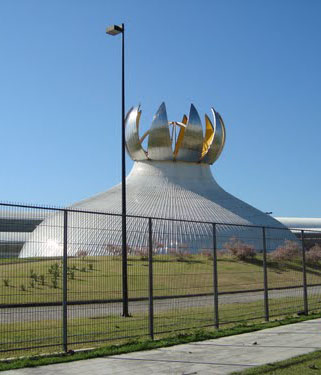
\includegraphics[width=0.30\textwidth]{sarahcupula.jpg}
         }
         \qquad
         
        \subfigure[Perspectiva TRT-Ba fonte: Acervo do Instituto Habitat]
           {\label{figura:trtcupula}
            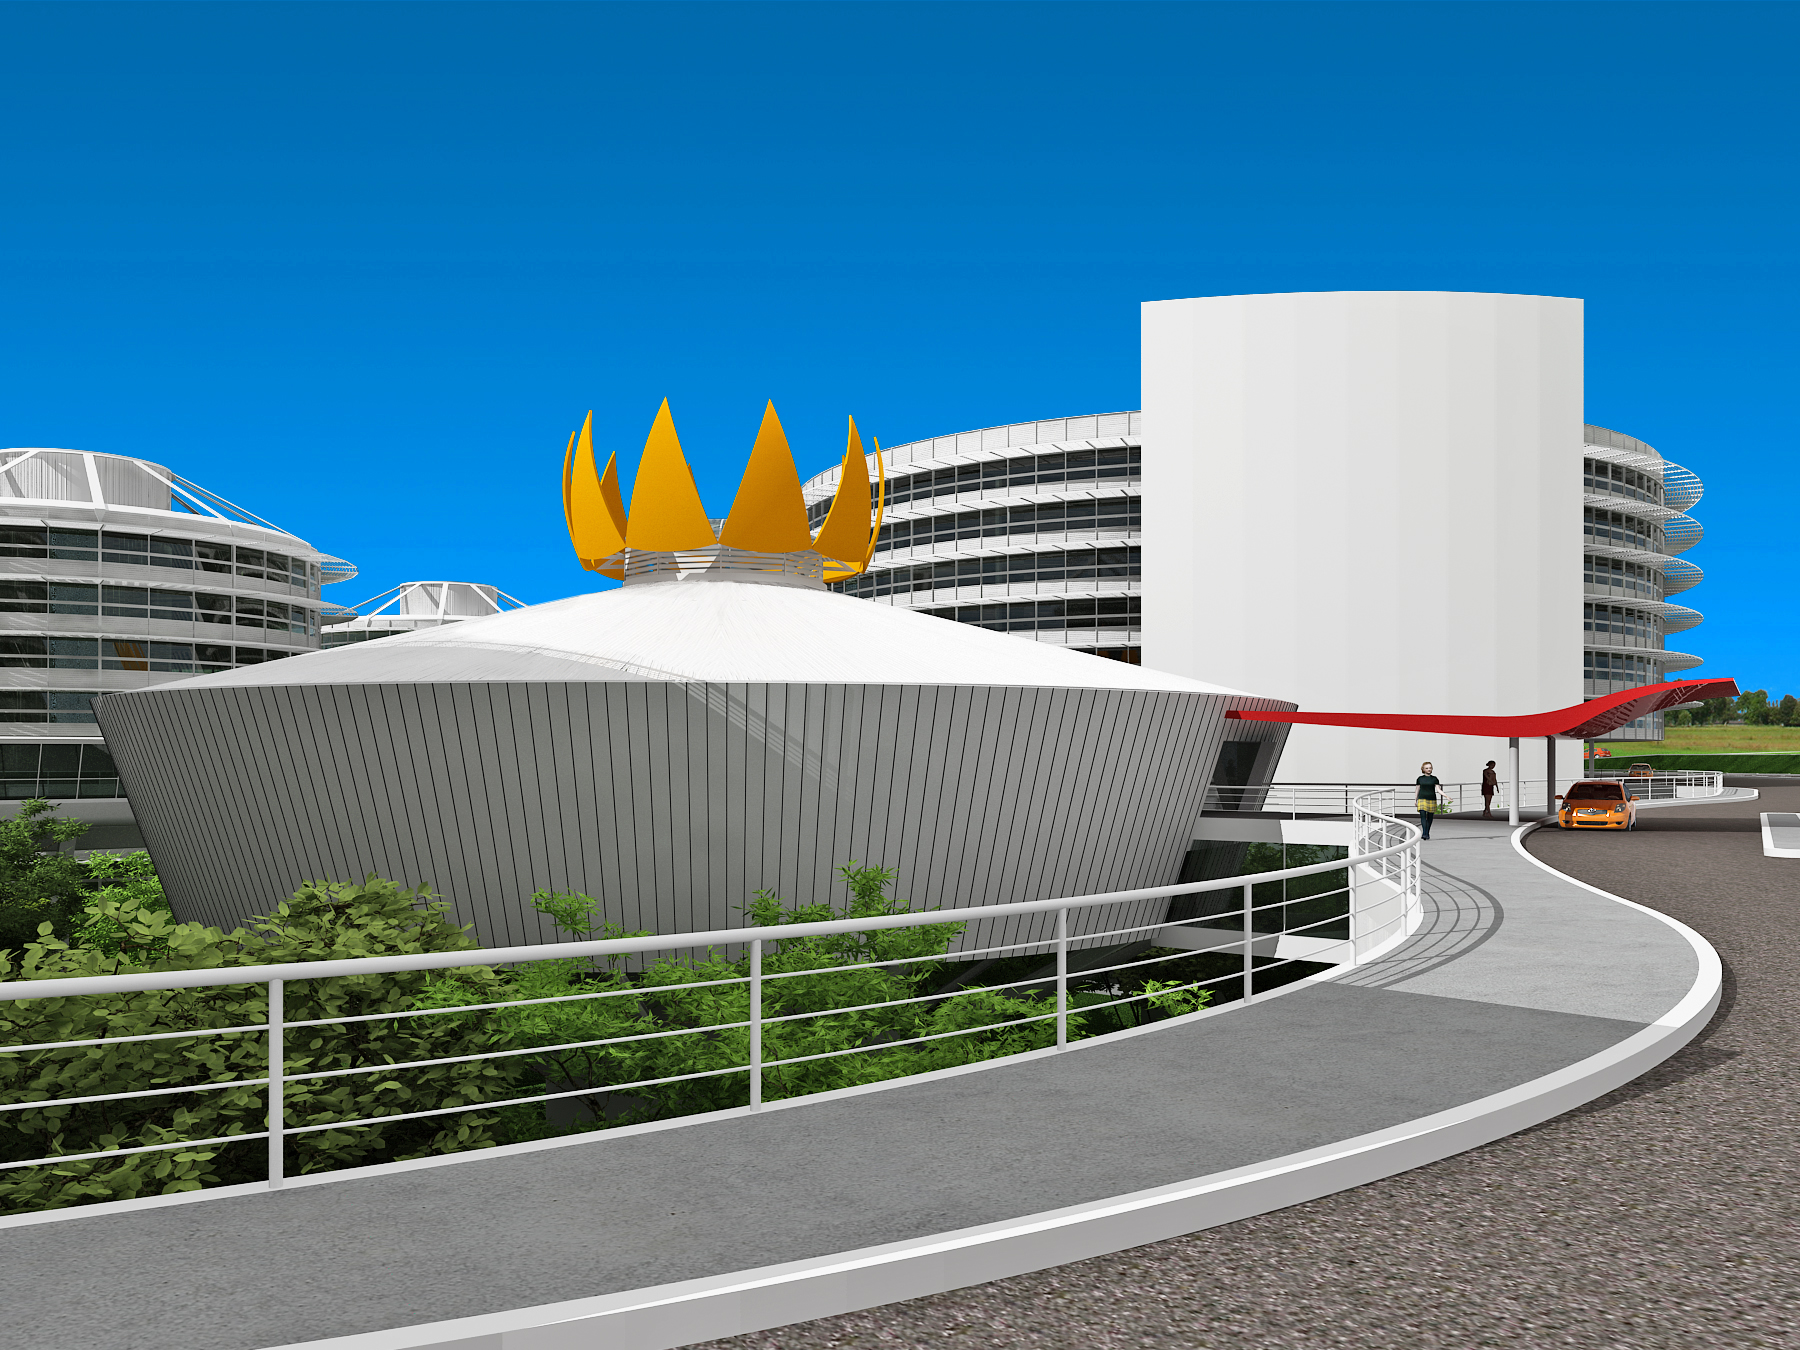
\includegraphics[width=0.47\textwidth]{trtcupula.jpg}
           }
       }

\end{center}
\caption{C�pulas m�veis do Arquiteto Jo�o Filgueiras Lima (Lel�)}
\label{figura:mprExemplos}
\end{figure}

As c�pulas m�veis permitem o controle da ilumina��o e exaust�o nos audit�rios. Possibilitando Tanto que ocorram de maneira natural, economizando energia, quanto artificiais, para que, por exemplo, se possa fazer melhor uso de m�dias projetadas em tel�es. O n�mero de p�talas, o raio de base da c�pula e a altura da calota esf�rica variam entre os dois projetos. Entre os par�metros passiveis de otimiza��o est�o: 

\begin{itemize}
\item o n�mero de p�talas;
\item o raio da base;
\item a altura da c�pula.
\end{itemize}

O n�mero de p�talas tem rela��o direta com os mecanismos (motores) de opera��o das c�pulas. Uma quantidade maior de p�talas, menor o peso de cada uma e um maior n�mero de motores el�tricos respons�veis pela articula��o de cada pe�a. O raio implica diretamente na �rea da abertura de ilumina��o e exaust�o. As tr�s vari�veis tem implica��o direta no aspecto visual da c�pula, sendo exigidas na abordagem do problema est�tico. O exemplo aqui proposto apresenta um algoritmo capaz de desenhar as c�pulas de ambos os projetos e varia��es destas. Al�m das tr�s vari�veis, duas foram acrescentadas: o ponto central do c�rculo de base da calota, e o �ngulo de rota��o da abertura das p�talas. O m�todo segue as seguintes etapas:

\begin{enumerate}
\item O c�rculo $C1$ � desenhado partindo do ponto central $PC$ com raio $r$.


\item $C1$ � dividido em $N$ partes iguais. Os pontos divisores s�o armazenados em uma lista de pontos $Lp1$, ordenados no sentido anti-hor�rio, partindo de um ponto inicial.

\item Cria-se um ponto $PH$ movendo o ponto $PC$ com uma dist�ncia $h$ ao longo do vetor perpendicular ao plano do c�rculo $C1$.

\item Uma lista de segmentos de reta $Llin1$ � criada ligando o ponto $PC$ a cada um dos pontos da lista $Lp1$.

\item Uma lista de arcos $Larc1$ � criada partindo do ponto $PH$ sendo tangente aos vetores representados pelos segmentos orientados da lista $Llin1$ e com ponto final os da lista $Lp1$.

\item uma lista de superf�cies $Ls1$ � criada pelo m�todo de revolu��o. Rotacionando os arcos da  lista $Larc1$ em torno de um eixo definido pelos pontos $PC$ e $PH$ ao longo de um �ngulo de $360/N$ e sentido anti-hor�rio.

\item uma lista de pontos $Lp2$ � criada a partir da lista $Lp1$ extraindo o primeiro elemento da lista e colocando no final: sendo a lista $Lp1$ composta por $Lp1_{0};Lp1_{1};Lp1_{2}...Lp1_{N}$ nesta ordem, em $Lp2$ os elementos de $Lp1$ na sequ�ncia $Lp1_{1};Lp1_{2}...Lp1_{N};Lp1_{0}$.

\item Uma lista de segmentos de reta $Llin2$ � criada ligando os pontos de mesmo �ndice das listas $Lp1$ e $Lp2$.
 
 \item O �ngulo $\alpha$ � definido pelo usu�rio. 
 
 \item Cada elemento da lista de superf�cies $Ls1$ � rotacionado um �ngulo $\alpha$ em torno do elemento correspondente da lista de segmentos de reta $Llin2$.
 
 \item Fim.

\end{enumerate}

\begin{figure}[!ht]
\begin{center}
  \mbox{
      \subfigure[]
         {
            \label{figura:cupula01}
            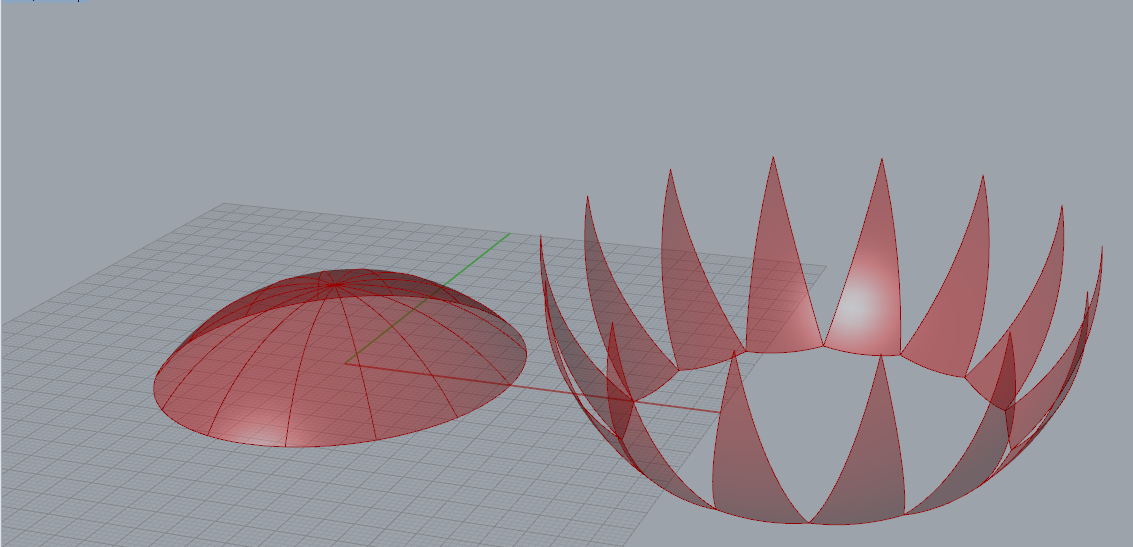
\includegraphics[width=0.45\textwidth]{cupula03.png}
         }
         
         
         

        \subfigure[]
           {
              \label{figura:cupula02}
              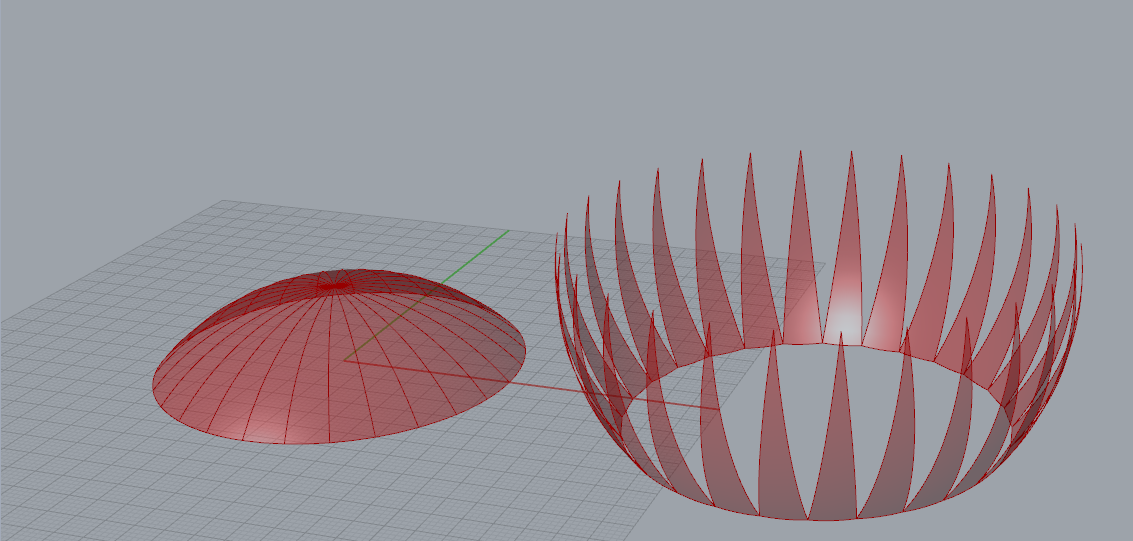
\includegraphics[width=0.45\textwidth]{cupula02.png}
           }
         }
         
  \mbox{
           \subfigure[]
                      {
                         \label{figura:cupula03}
                         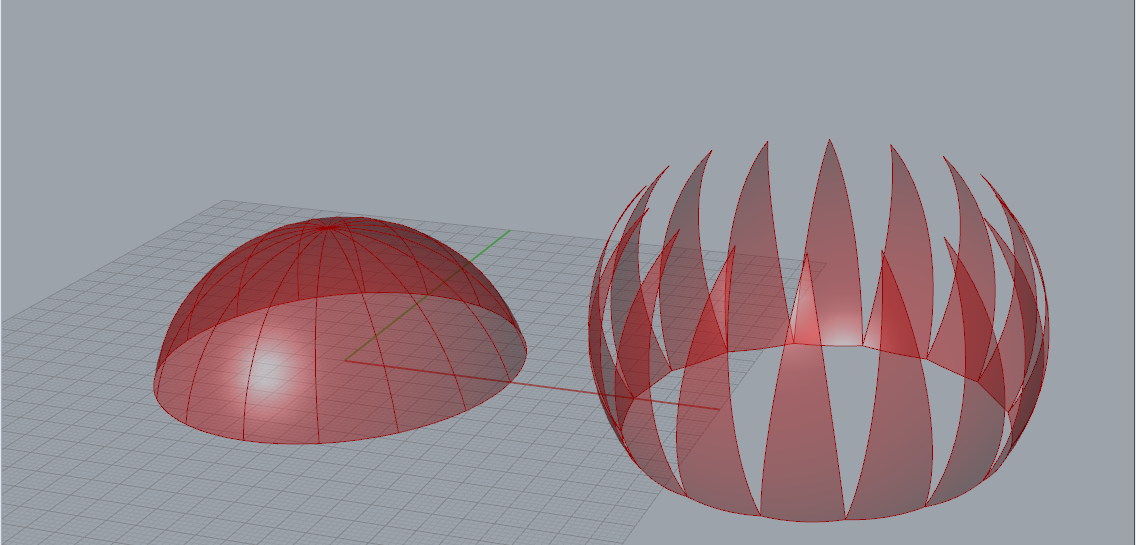
\includegraphics[width=0.45\textwidth]{cupula01.png}
                      }
                      
                      
           \subfigure[]
                                 {
                                    \label{figura:cupula04}
                                    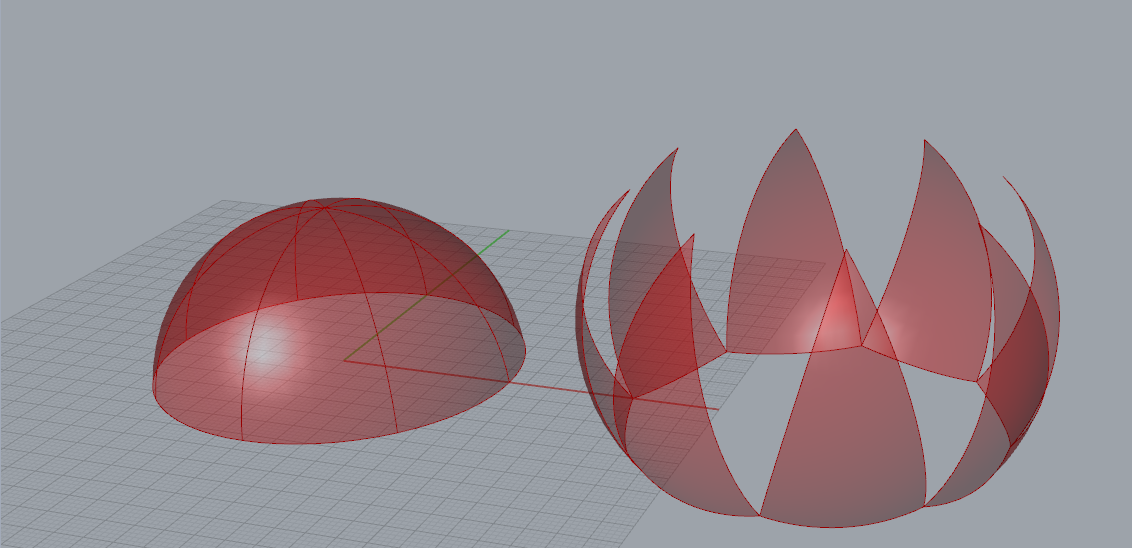
\includegraphics[width=0.45\textwidth]{cupula04.png}
                                 }
       }
\mbox{
           \subfigure[]
                      {
                         \label{figura:cupula05}
                         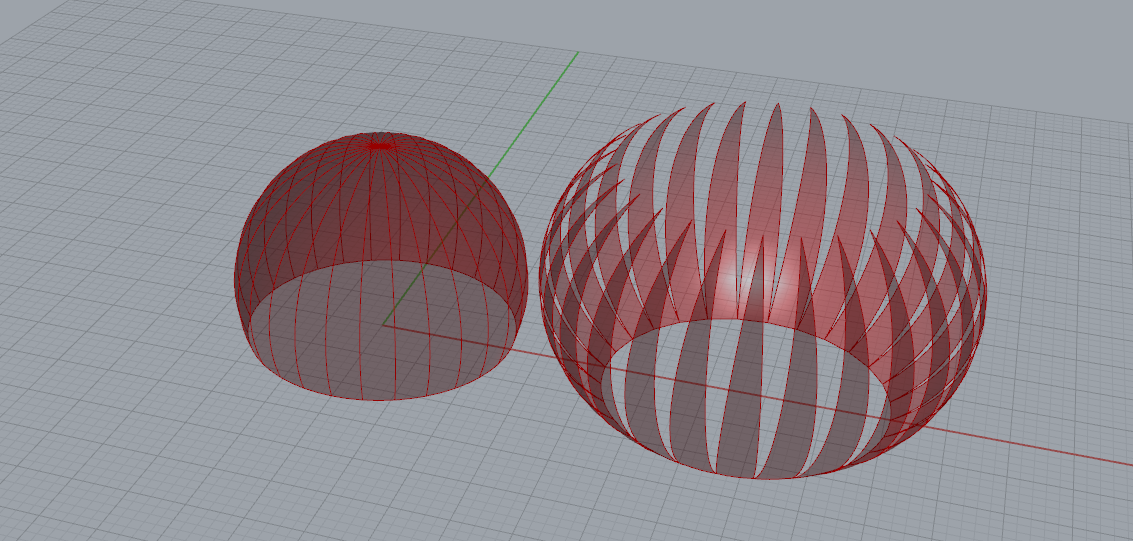
\includegraphics[width=0.45\textwidth]{cupula06.png}
                      }
                      
                      
           \subfigure[]
                                 {
                                    \label{figura:cupula06}
                                    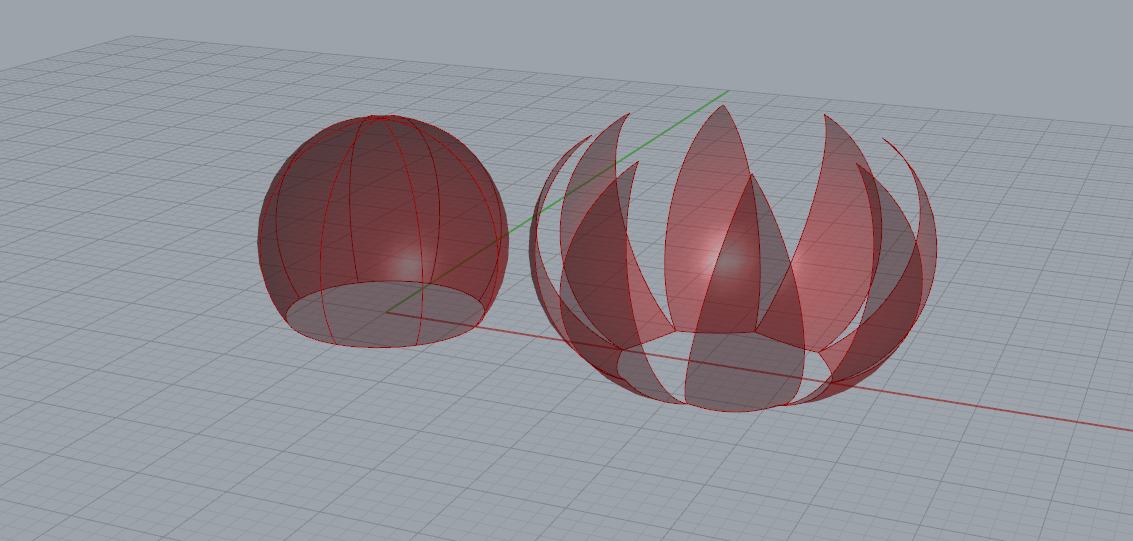
\includegraphics[width=0.45\textwidth]{cupula05.png}
                                 }
    }
 

\end{center}
\caption{C�pulas m�veis geradas por MPR - \textit{Rhinoceros/Grasshopper} }
\label{figura:exemplocupgrass}
\end{figure}


O algoritmo foi implementado no ambiente \textit{Rhinoceros/Grasshopper} e pode ser visto no Ap�ndice \ref{Apend2:cupula}. A Figura \ref{figura:exemplocupgrass} mostra algumas formas geradas pelo processo. Os par�metros de entrada s�o: o ponto $PC$, o raio $r$, a dist�ncia de deslocamento $h$, o n�mero de p�talas $N$ e o �ngulo de rota��o $\alpha$. A cria��o do ponto $PH$, perpendicular ao plano do c�rculo $C1$, � uma exemplo de restri��o. O m�todo de cria��o das geratrizes $Larc1$, em fun��o das tangentes dos vetores em $Llin1$, restringe a forma da c�pula fechada � uma calota esf�rica, com ponto central pertencente � reta que passa pelos pontos $PC$ e $PH$.

Aproximando-se do conceito de demonstra��o de um teorema em Geometria, nota-se uma importante rela��o entre vari�veis $r$ e $h$:
\begin{itemize}
\item sempre que $r$ for igual � $h$, a calota � uma semiesfera e o centro da esfera coincide com o ponto $PC$;
\item sempre que $r$ for maior que $h$, a calota � menor do que a metade da esfera e o seu centro est� abaixo do ponto $PC$;
\item sempre que $r$ for menor que $h$, a calota � maior do que a metade da esfera  seu centro est� acima do ponto $PC$;
\item quando o valor de $r$ ou de $h$ � igual a zero, o algoritmo falha na gera��o de formas, tornando essas configura��es invalidas para a solu��o do problema.  
\end{itemize}

Ampliando essas rela��es para todo o conjunto de par�metros, � poss�vel afirmar que, para cada configura��o v�lida destes, existe uma  �nica c�pula como resposta. O mesmo pode ser dito para qualquer MPR que n�o utilize, de alguma forma, a aleatoriedade em seu conjunto de regras. Cada p�tala � representada computacionalmente como uma curva \textit{nurbs} e, assim como cada uma das geometrias auxiliares utilizadas pelo algoritmo, � composta por um conjunto de vari�veis cujos valores s�o definidos pela atua��o do \textit{constraint solvers}. Os par�metros s�o vari�veis especiais que alimentam e manipulam o conjunto de restri��es que guiam a cria��o das formas.

Enquanto os par�metros de entrada podem ser dinamicamente modificados pelo usu�rio, as restri��es s� podem ser alteradas pela modifica��o do algor�timo. A cria��o das formas � guiada por um di�logo entre os valores explicitamente controlados pelos projetistas e as restri��es impostas pelas regras transcritas no algoritmo. Enquanto os primeiros garantem a cria��o de variedade pela simples altera��o de valores, tamb�m chamadas de flex�es do modelo, as �ltimas garantem que a forma gerada faz parte de um conjunto de resultados espec�ficos, compat�veis com o problema abordado, e apresenta as inten��es de projeto, n�o como forma, mas como ideia. 



    % !TeX encoding = ISO-8859-1
% !TeX spellcheck = pt_BR
\chapter{Grafost�tica}
\label{chapter:grafostatica}

\begin{flushright}
  "\textit{Los que buscan las leyes de la Naturaleza \\
  como un apoyo para sus nuevas obras\\ colaboran con el creador.\\ 
  Copiadores no colaboran.\\
   Debido a esto, la originalidad\\consiste en regresar al origen.}"
  \\(Antoni Gaud�)
\end{flushright}


A origem da Geometria est� intimamente ligada com as primeiras civiliza��es humanas. Reconhecendo as dificuldades de estabelecer um consenso em torno das origens da Matem�tica (Aritm�tica e Geometria), \citeonline[p. 4]{boyer1974} apontam �s teorias antag�nicas de Her�doto e Arist�teles como as hip�teses mais aceitas para o surgimento da Geometria. Her�doto acreditava que a origem estava ligada � necessidade pr�tica de se fazer novas medidas de terra, ap�s cada inunda��o anual, no vale do antigo Egito. Enquanto Arist�teles creditava � classe sacerdotal eg�pcia, que a teria criado para aprecia��o do belo. E lembram o fato dos ge�metras do Egito serem frequentemente chamados de "esticadores de corda" como um apoio comum as duas teorias, j� que essas eram esticadas tanto para demarcar terras, quanto para marcar as bases dos templos. Em ambos os exemplos a atividade de construir est� presente.

\citeonline{ceccato2010mbg} chama aten��o para o significado das palavras "arquiteto" (mestre construtor) e Geometria (medida da terra) para afirmar que ge�metras e arquitetos eram, primordialmente, a mesma pessoa. A liga��o entre Geometria e constru��o s�o evidentes e profundas, mesmo tendo em conta a subdivis�o em diversas profiss�es pela qual a atividade de construir passou ao longo de s�culos. Antes do desenvolvimento da Mec�nica dos Materiais (por volta do s�culo XIX), a constru��o de estruturas era guiada por um conhecimento emp�rico das propor��es entre esfor�os e materiais \cite{mccormac2009}.

\section{Est�tica e Grafost�tica}
\label{section:EstaGrafo}

A Mec�nica � o ramo da F�sica que estuda o movimento e repouso e divide-se em Cinem�tica e Din�mica. Enquanto a primeira se debru�a sobre o movimento sem abranger as suas causas, a segunda trata do efeito das for�as sobre o movimento e repouso dos corpos, e se divide em Cin�tica e Est�tica. \citeonline{johnson1908} aponta m�todos alg�bricos ou gr�ficos podem ser alternadamente mais eficazes  para a resolu��o de determinados problemas da Est�tica, definida como o ramo da Din�mica que estuda o equil�brio dos corpos. Desde ent�o, pouco mudou nas bases e defini��es dos problemas da Mec�nica aplicada �s constru��es, mas diferen�as significativas aparecem nos m�todos e ferramentas de trabalho dos profissionais envolvidos.

\begin{quotation}
\textbf{Grafost�tica}, ou \textbf{Est�tica Gr�fica}, estuda os problemas de Est�tica por m�todos puramente geom�tricos. � de grande utilidade em Resist�ncia dos Materiais para a determina��o das rea��es, esfor�os cortantes, momentos fletores, flechas e, nos sistemas articulados, para a an�lise dos esfor�os interiores que acontecem nas barras dos mesmos. \cite{sanjuan1951}
\end{quotation}

As ferramentas anal�ticas e gr�ficas de c�lculo estrutural foram desenvolvidas paralelamente ao longo do s�culo XIX. Trabalhos como o de James Clerk \citeonline[p.451-525]{maxwell1965} s�o citados tanto como fundamentais na evolu��o da teoria do c�lculo estrutural modero \cite{mccormac2009}, quanto fundador dos procedimentos geom�tricos de resolu��o dos problemas de Est�tica, desenvolvidos principalmente pelos trabalhos de Culmann (1866) e \citeonline{cremona1890graphical} \cite{johnson1908} \cite{gerhardt2003} 
\cite{aag2010193}. 

A medida que ferramentas num�ricas, tanto mec�nicas (e.g. r�gua de c�lculo) mas principalmente computacionais crescem em efici�ncia \cite{baumgart2000} e uma tend�ncia anal�tica se desenha na engenharia \cite{gerhardt2003}, a Est�tica Gr�fica perde espa�o e passa a ser encarada quase que apenas como um instrumento did�tico para o entendimento da Mec�nica, como no livro de \citeonline{costa1974}.

O posterior desenvolvimento da computa��o gr�fica acabou demonstrando que, tamb�m no ambiente computacional, o m�todo anal�tico nem sempre � a maneira mais eficaz de se abordar um problema. O exemplo mais not�rio provavelmente est� na descoberta dos fractais por Mandelbrot. Embora, no experimento que deu origens � este desenvolvimento cient�fico, fun��es estivessem sendo calculadas atrav�s de m�todos num�ricos e vertidos em gr�ficos por um processo de mesma natureza, o avan�o no conhecimento acontece pela inspe��o do olhar humano sobre os desenhos dos resultados, padr�es s�o encontrados, estudados e uma ferramenta matem�tica � testada e aceita para medir as caracter�sticas destas novas geometrias. 

Sobre a Grafost�tica, surge a hip�tese de que o uso das ferramentas computacionais gr�ficas para o aux�lio � tomada de decis�es sobre formas geom�tricas edific�veis, � capaz de trazer uma compreens�o mais ampla, objetiva e clara para o estudo, ensino e pr�tica das quest�es estruturais. As vantagens cognitivas de utilizar formas geom�tricas (diagramas), em oposi��o ao uso de express�es matem�ticas, para a an�lise de outras formas (constru��o) � evidente.

Entre os defensores desta hip�tese, \citeonline{gerhardt2003} apontam as virtudes do m�todo al�m dos exemplos did�ticos. Estabelece rela��o direta entre o uso hist�rico da ferramenta e a maneira como ela � capaz de guiar o projetista pelo espa�o de solu��es poss�veis, destacando os trabalhos de Anton� Gaud� e Gustave Eiffel. Um exemplo de utiliza��o da Grafost�tica em ambiente CAD � apresentado no projeto de refor�o estrutural em um pr�dio da prefeitura de Berlim, onde a proposta executada � enxergada apenas depois de se analisar os diagramas constru�dos atrav�s do m�todo. \citeonline{Block2006} aplicam mecanismos da Grafost�tica na elabora��o de uma estrat�gia computacional para an�lise em tempo real de projetos com estruturas em pedra. \citeonline{Tessmann2008} elenca a Est�tica Gr�fica entre as ferramentas eficientes para aprimoramento do di�logo entre projetistas de arquitetura e de estrutura. \citeonline{Zanni2009} trabalham em um modelo computacional gr�fico para an�lise de estruturas submetidas � carregamento axial. \citeonline{Shearer2010} prop�e algoritmos para automa��o do desenho de diagramas da Grafost�tica e \citeonline{aag2010193} defendem cria��o de uma ferramenta din�mica para gera��o dos mesmos, recebendo informa��es de um MPR. \citeonline{Harding2012} aponta que a Grafost�tica de Culmann serve de base para alguns algoritmos computacionais din�micos de explora��o interativa 2D de estruturas e prop�e um algoritmo que adicione o eixo $z$ no c�lculo. O trabalho de \citeonline{Block2009}, aplica a Est�tica Gr�fica como ferramenta para "encontrar" interativamente estruturas submetidas unicamente � compress�o (\textit{form finding}).

\section{Precis�o do M�todo}
\label{section:precisao}

A precis�o dos m�todos gr�ficos aplicados ao c�lculo de estruturas � demonstrado por diversos autores. \citeonline[p. 30]{panseri1952} mostra que apenas duas ou tr�s casas decimais s�o plenamente satisfat�rios quando levadas em conta as toler�ncias de fabrica��o, as incertezas que envolvem certos esfor�os e os coeficientes de seguran�a necess�rios para a eficiente execu��o de um elemento construtivo. \citeonline[p. 2]{johnson1908} afirma que, embora os dois m�todos sejam cientificamente corretos, a precis�o do processo anal�tico depende da quantidade de casas decimais e algarismos significativos envolvidos. Na resolu��o gr�fica, as habilidades de desenho e os limites da vis�o humana tem car�ter determinante na acuidade do c�lculo.

\begin{figure}[!ht]
\begin{center}
  \mbox{
      \subfigure[C�lculo de rea��es em uma viga simples - fonte: \citeonline{sanjuan1951} ]
         {\label{figura:exemploprecisao1}
          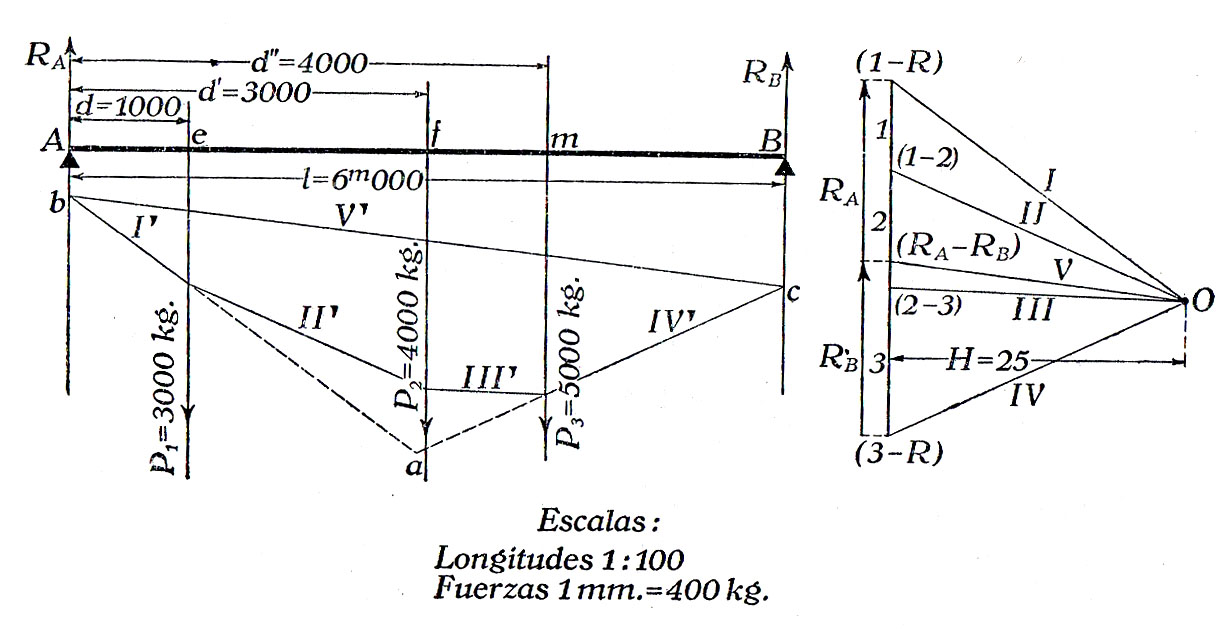
\includegraphics[width=0.40\textwidth]{exemploprecisao1.jpg}
         }
         
         
        \subfigure[C�lculo de rea��es em uma viga simples executado no Rhino3D ]
           {\label{figura:exemploprecisao2}
            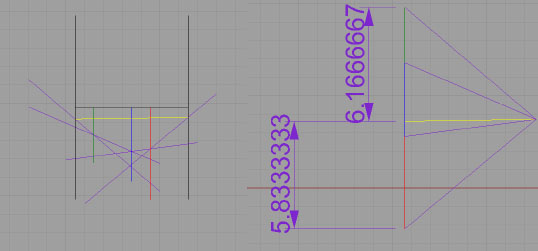
\includegraphics[width=0.40\textwidth]{exemploprecisao2.jpg}
           }
       }

\end{center}
\caption{Precis�o do c�lculo}
\label{figura:exemploprecisao}
\end{figure}

Utilizando a Grafost�tica em ambiente computacional as diferen�as praticamente desaparecem. A Figura \ref{figura:exemploprecisao1} � um problema apresentado por \citeonline[p. 16]{sanjuan1951} onde o mesmo c�lculo de rea��es � feito de maneira anal�tica e gr�fica, apresentando pequenas varia��es entre os resultados. O mesmo problema solucionado graficamente em um programa CAD (Figura \ref{figura:exemploprecisao2} ) tem os mesmos valores da resolu��o anal�tica se executado em uma calculadora com mesmo n�mero de casas decimais utilizadas pelo CAD. 

Embora a Est�tica Gr�fica sirva como base cient�fica do experimento, em um n�vel mais baixo s�o opera��es num�ricas que realizam o c�lculo. A habilidade com os instrumentos de desenho � substitu�da pelo cuidado na aplica��o do comando correto. O espa�o cartesiano implementado no computador pode esconder erros relacionados as vari�veis de ponto flutuante, mas felizmente, as precau��es que devem ser tomadas s�o as mesmas que devem ser adotadas para o desenho t�cnico em CAD. Se, no final do s�culo XIX, muitos engenheiros e arquitetos enxergavam os benef�cios de associar seu instrumento de projeto (a prancheta) com uma ferramenta de c�lculo, semelhantes vantagens podem ser usufru�das por usu�rios experientes nos atuais e precisos sistemas  de projeto assistido por computador.

\section{Conceitos Fundamentais da Est�tica}
\label{section:conceitosestatica}

\begin{itemize}
\item \textbf{Corpo R�gido:} � um corpo que n�o sofre altera��es de forma ou tamanho sob a a��o de uma for�a ou sistema. Embora n�o exista na natureza um material com essas propriedades, para efeito pr�tico, a grande maioria dos materiais construtivos funcionam como um corpo r�gido, em um contexto maior ou menor.
\item \textbf{Repouso:} a rela��o existente entre dois pontos quando uma linha imagin�ria conectando-os n�o apresenta mudan�as em comprimento ou dire��o.
\item \textbf{Movimento:} Quando a linha imagin�ria descrita acima muda. As mudan�as no comprimento s�o chamadas de \textbf{transla��o}, na dire��o, de \textbf{rota��o}
\item \textbf{For�a:} A��o que causa (ou tende � causar) modifica��o no movimento de  um corpo. Entendidas como o ato de puxar ou empurrar, as for�as s�o grandezas vetoriais, e como tais possuem tr�s elementos essenciais:
\subitem \textbf{M�dulo ou Magnitude:} � um valor num�rico real que mede a capacidade de uma for�a em produzir movimento, quando comparado com uma for�a padr�o escolhida. Por defini��o, este valor n�o possui nota��o de positivo ou negativo.
\subitem \textbf{Dire��o:} a dire��o da linha sob a qual a for�a tende a produzir movimento.
\subitem \textbf{Sentido:} para qual dos extremos da dire��o a for�a tende a produzir movimento.
\item \textbf{Representa��o Gr�fica de Vetores:} � dada atrav�s de segmentos orientados. Um dos pontos extremos do segmento � tomado como ponto inicial e o outro como final, definindo assim um sentido. O m�dulo � representado pelo comprimento e a dire��o pela reta que contem o segmento, bem como as paralelas � ela.
\item \textbf{Ponto de Aplica��o:} o ponto do corpo em que a for�a age.
\item \textbf{Linha de A��o:} a dire��o do vetor for�a que passa pelo seu ponto de aplica��o. No caso de um corpo r�gido, um outro \textbf{ponto de aplica��o} pode ser considerado em qualquer local sobre a linha de a��o de uma for�a, produzindo o mesmo efeito.
\item \textbf{Composi��o de Vetores:} para um sistema vetorial qualquer(\textbf{componentes}), a composi��o consiste em encontrar o vetor (\textbf{resultante}) que tende a produzir o mesmo efeito quando aplicado sobre um corpo. Diz-se que as componentes e sua resultante s�o vetorialmente \textbf{equivalentes}. Tamb�m chamada de \textbf{soma de vetores}, a composi��o � graficamente executada posicionando as componentes de forma que o extremo final do vetor anterior encontre o extremo inicial do vetor seguinte. A resultante � o segmento orientado que tem o mesmo ponto inicial do primeiro vetor e o ponto final do �ltimo.
\item \textbf{Resolu��o de Vetores:} para um vetor qualquer, encontrar dois ou mais componentes cuja soma tenha por resultante o vetor dado.
\item \textbf{Equilibrante:} for�a que equilibra o sistema. Possui o mesmo mesmo m�dulo e dire��o e linha de a��o do vetor resultante, porem com sentido oposto.
\item \textbf{Bin�rios:} duas for�as iguais (m�dulo e dire��o) e de sentidos opostos, com linhas de a��o paralelas sobre o mesmo corpo. Os bin�rios apresentam unicamente a tend�ncia de produzir rota��o. A medida desta tend�ncia � chamada de \textbf{momento do bin�rio}, que � calculada pela multiplica��o do m�dulo de uma das for�as pela dist�ncia ortogonal entre suas linhas de a��o
(bra�o), em unidade apropriada.

\end{itemize}

 
\section{Diagramas Rec�procos}
\label{section:diagramasreciprocos}

A Grafost�tica baseia seus algoritmos de c�lculo nos chamados diagramas rec�procos, que consistem em apresentar o mesmo sistema de for�as em duas figuras complementares. Em uma temos os vetores das for�as atuantes sobre um corpo r�gido, grafados em magnitude, dire��o, sentido e representados na posi��o de soma (Figura \ref{figura:poligonodeforcas}), essa figura � referida como pol�gono de for�as (PF). Para a determina��o do m�dulo uma escala que relaciona for�a e medida � eleita (e.g. $ \dfrac{1 cm}{10 Kgf} $) de forma semelhante ao procedimento de desenho t�cnico em escala. No segundo diagrama, chamado de forma geom�trica (FG) ou plano de situa��o (Figura \ref{figura:formageometrica}), apenas as linhas de a��o s�o representadas.

\begin{figure}[!ht]
\begin{center}
  \mbox{
      \subfigure[Pol�gono de For�as]
         {\label{figura:poligonodeforcas}
          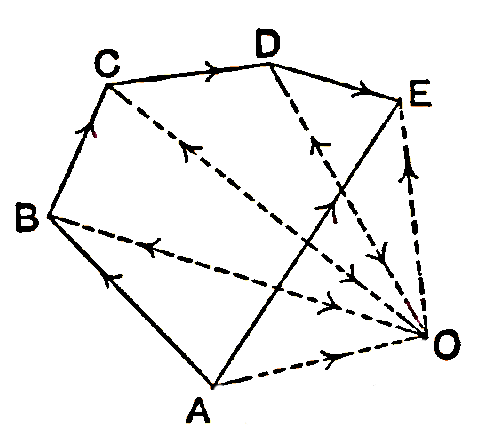
\includegraphics[width=0.45\textwidth]{poligonodeforcas.png}
         }
         
         
        \subfigure[Forma Geom�trica]
           {\label{figura:formageometrica}
            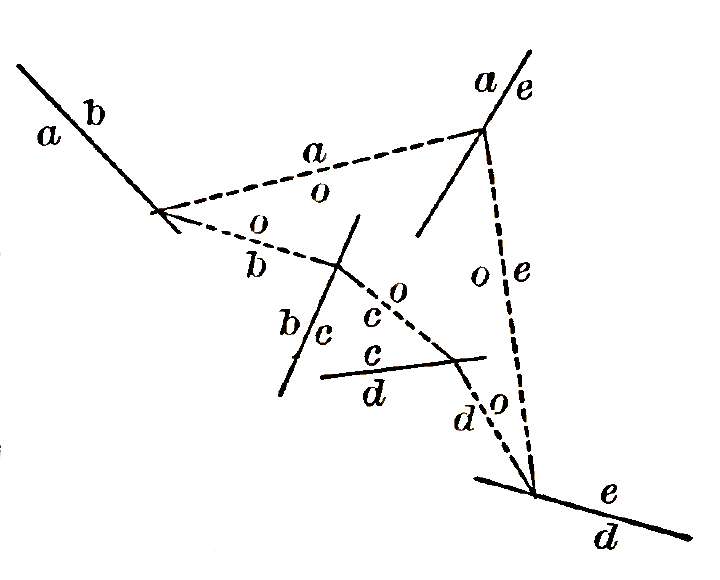
\includegraphics[width=0.45\textwidth]{formageometrica.png}
           }
       }

\end{center}
\caption{Diagramas Rec�procos - fonte: \citeonline{Hoskins1899} (editado)}
\label{figura:driagramasreciprocos}
\end{figure}


Partindo do sistema da Figura \ref{figura:driagramasreciprocos}, considerando um conjunto de quatro for�as, representadas por $AB, BC, CD$ e $DE$ no pol�gono de for�as, e cujas respectivas linhas de a��o s�o $ab, bc, cd$ e $de$ na rec�proca forma geom�trica (nota��o de Bow \cite[p. 5-7]{burr}), o c�lculo da resultante $AE$ e da sua linha de a��o $ae$ � feito pelos seguintes passos:


\begin{enumerate}
\item Um ponto qualquer, chamado de polo, representado por $O$ � escolhido no pol�gono de for�as. 
\item Os raios polares, linhas partindo do ponto $O$ para cada um dos pontos $A, B, C, D$ e $E$  s�o desenhados.
\item A reta $oa$, paralela � $OA$ � tra�ada na forma geom�trica partindo de um ponto qualquer na linha de a��o $ab$.
\item Pelo mesmo ponto que $oa$ intercepta $ab$, a reta $ob$ paralela � $OB$ � tra�ada.
\item A reta $oc$, paralela a $OC$ � tra�ada  partir do ponto em que $ob$ intercepta $bc$. O passo � repetido para $od$ partindo da intercess�o de $oc$ e $cd$, e para $oe$ por $od$ e $de$.
\item O vetor $AE$ � determinado pela liga��o dos pontos $A$ e $E$ no pol�gono de for�as.
\item A dire��o $ae$ � tra�ada por uma paralela � $AE$ passando pelo ponto intercess�o das retas $oa$ e $oe$ na forma geom�trica.  
\end{enumerate}

A poligonal formada por $oa, ob, oc, od,$ e $oe$ � chamada de pol�gono funicular, e seus lados s�o as denominados de cordas \cite[p. 16]{Hoskins1899} ou linhas de press�o \cite{costa1974}. Para cada polo $O$ escolhido aleatoriamente um funicular diferente � constru�do. Para o sistema apresentado na Figura \ref{figura:driagramasreciprocos}, as intercess�es de  $oa$ e $oe$ referentes ao polo $O$ e a um outro polo qualquer $O'$ estar�o necessariamente sobre a linha de a��o $ae$, uma alternativa para o c�lculo. 

\section{Condi��es de Equil�brio}
\label{section:condicaodeequilibrio}
No m�todo anal�tico, as condi��es de equil�brio de um corpo r�gido submetido a um sistema de for�as � que, tanto o somat�rio dos momentos, quanto o das transla��es seja igual a zero (equa��o \ref{equacao:equilibrio}).


\begin{equation}
\label{equacao:equilibrio}
 \sum{M}=0  \qquad \sum{T}=0 
\end{equation}


Na Grafost�tica, a an�lise do equil�brio � feita pela observa��o do pol�gono de for�as e do funicular.

\begin{itemize}
\item Se PF � um pol�gono fechado, o sistema est� em equil�brio de transla��o.

\item Se o funicular � um pol�gono fechado, o sistema est� em equil�brio de rota��o.

\item Se o PF � fechado e o funicular aberto e de lados opostos paralelos, a resultante do sistema � um bin�rio. O corpo r�gido submetido a estas for�as est� em equil�brio de transla��o, mas est� submetido a um momento. Neste caso, os raios polares extremos ser�o iguais, e o valor do momento ser� dado pelo produto do comprimento de um dos raios polares extremos pela dist�ncia entre as paralelas das cordas extremas.

\end{itemize}

As propriedades dos diagramas rec�procos est�o ligadas ao fato destes serem representa��es gr�ficas de aspectos complementares da an�lise de for�as. O pol�gono de for�as trata da soma dos vetores, um PF fechado implica em um somat�rio de resultante nula para o sistema. O equil�brio de transla��o pode ser assim verificado, por�m a rota��o, os bin�rios e seus momentos precisam de informa��es quando � posi��o no espa�o, pontos de aplica��o e linhas de a��o das for�as, fornecidas pela forma geom�trica. Os raios polares relativos a pontos consecutivos do PF podem ser entendidos como componentes da for�a representada entre esses pontos (considerando o sentido a partir do polo para o primeiro e sentido em dire��o ao polo para o segundo). A utiliza��o de intercess�es entre linhas de a��o do FG corresponde ao princ�pio da Est�tica que afirma, sobre o estudo dos corpos r�gidos, que qualquer ponto sobre a linha de a��o de uma for�a pode ser adotado como ponto de aplica��o produzindo o mesmo efeito. As propriedades dos diagramas rec�procos podem ser experimentadas atrav�s do algoritmo no Ap�ndice \ref{Apend1:funicular1}, cujo funcionamento foi registrado e comentado no v�deo \href{https://www.youtube.com/watch?v=pIa0o2M0-_s}{01 - Propriedades dos PF, FG e Funiculares} em anexo.


\section{Problemas em Equil�brio}
\label{section:resolucaodeproblemas}
Os problemas de Est�tica consistem em determinar os elementos desconhecidos (magnitudes, dire��es, sentidos, linhas de a��o e ponto de aplica��o) em sistemas de for�as que est�o sabidamente em equil�brio. \citeonline{johnson1908} apresenta os problemas fundamentais da seguinte maneira:

\begin{enumerate}
\item encontrar a magnitude, dire��o e ponto de aplica��o de uma for�a de um sistema;

\item magnitude de duas for�as de um sistema;

\item magnitude de uma for�a e magnitude e dire��o de outra do mesmo sistema;

\item magnitude de tr�s for�as do mesmo sistema.

\end{enumerate}

Uma abordagem did�tica, que permite ao leitores antever os valores desconhecidos que deveram ser determinados pela Grafost�tica em cada situa��o. As opera��es necess�rias para encontrar esses valores, representam a solu��o dos quatro casos que formam a base dos problemas da Est�tica, cuja formula��es e solu��es gr�ficas ser�o apresentadas e comentadas em seguida.

\subsection{Caso Um - Composi��o de uma For�a}
\label{section:prob1}


O primeiro caso � basicamente o c�lculo da resultante apresentado na Se��o \ref{section:diagramasreciprocos}. Mas � importante saber que, al�m da resultante, este problema fundamental tamb�m � usado para o c�lculo da equilibrante do sistema. Partindo da Figura \ref{figura:driagramasreciprocos}, o primeiro passo para encontrar a for�a que equilibra o sistema � justamente o c�lculo da resultante, seguindo a sequ�ncia de instru��es apresentada. Na forma geom�trica, a linha de a��o $ae$ � a mesma para a resultante e equilibrante do sistema. No pol�gono de for�as contudo, o equil�brio se d� pela atua��o da for�a de mesmo m�dulo e dire��o que a resultante $AE$ porem com o sentido oposto. Portanto o vetor $EA$ tem m�dulo, dire��o e sentido, bem como ponto te aplica��o $ea$ para a resolu��o do caso.

\subsection{Caso Dois - Resolu��o de uma For�a em Duas Componentes}
\label{section:prob2}

O segundo caso � dividido em dois problemas: o primeiro trata de for�as concorrentes, o segundo, considerado uma situa��o especial, trata de um conjunto de for�as onde todas, inclusive as duas de magnitude desconhecidas, s�o paralelas.


\begin{figure}[!ht]
\begin{center}
  \mbox{
      \subfigure[Pol�gono de For�as]
         {\label{figura:pf2a}
          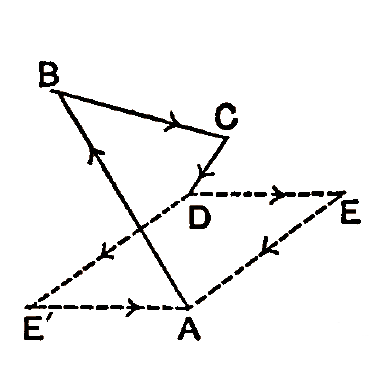
\includegraphics[width=0.40\textwidth]{pf2a.png}
         }
         
         
        \subfigure[Forma Geom�trica]
           {\label{figura:fg2a}
            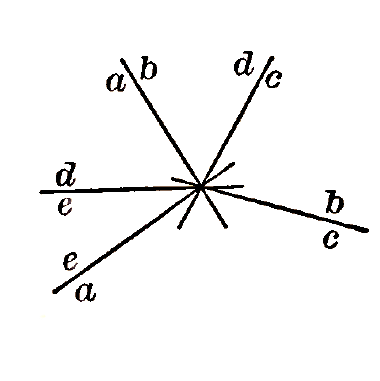
\includegraphics[width=0.40\textwidth]{fg2a.png}
           }
       }

\end{center}
\caption{Caso 2 -  for�as concorrentes - fonte: \citeonline{Hoskins1899}}
\label{figura:caso2a}
\end{figure}

No caso de for�as concorrentes, ilustrado na Figura \ref{figura:caso2a}, onde s�o plenamente conhecidas as for�as $AB, BC$ e $CD$, e pretende-se encontrar as magnitudes de $DE$ e $EA$. O primeiro passo � desenhar todas as linhas de a��o no FG (Figura \ref{figura:fg2a}). Em seguida, desenha-se as for�as totalmente conhecidas no PF. Sabendo que o sistema est� em equil�brio, infere-se que o PF tem que ser um pol�gono fechado. Tra�ando uma paralela � $de$ pelo ponto $D$ e uma � $ea$ pelo ponto $A$, observa-se que o ponto de encontro dessas duas retas � o ponto $E$. O PF se fecha e s�o determinadas as magnitudes $DE$ e $EA$. O ponto $E'$ pode ser constru�do tra�ando-se uma paralela � $EA$ pelo ponto $D$ e uma paralela � $DE$ pelo ponto $A$ e tamb�m � admitido como solu��o do problema, os mesmos vetores s�o encontrados em magnitude e sentido, tendo por dire��o as retas que cada uma delas � paralela. Deve-se contudo, atentar para que n�o haja conflito com a nomenclatura dos vetores nos diagramas rec�procos. 

\begin{figure}[!h]
\begin{center}
  \mbox{
      \subfigure[Pol�gono de For�as]
         {\label{figura:pf2b}
          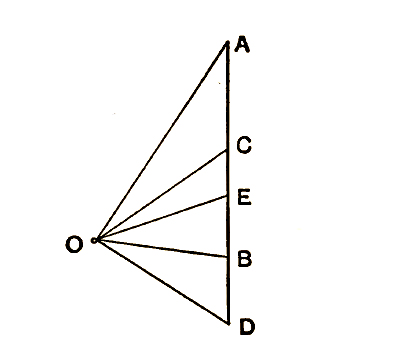
\includegraphics[width=0.40\textwidth]{pf2b.png}
         }
         
         
        \subfigure[Forma Geom�trica]
           {\label{figura:fg2b}
            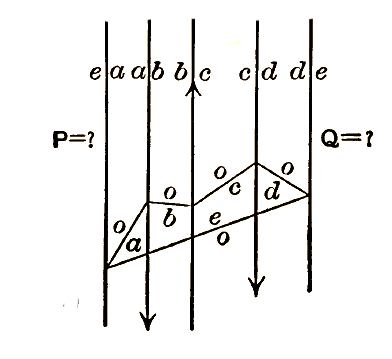
\includegraphics[width=0.40\textwidth]{fg2b.png}
           }
       }

\end{center}
\caption{Caso 2 - for�as paralelas - fonte: \citeonline{johnson1908}}
\label{figura:caso2b}
\end{figure}

Para um sistema de for�as paralelas (Figura \ref{figura:caso2b}) tomemos por vetores totalmente conhecidos $AB, BC$ e $CD$, com suas respectivas linhas de a��o tra�adas na figura \ref{figura:fg2b}. No PF, tra�a-se as for�as $AB, BC$ e $CD$, bem como seus respectivos raios polares relativos � um polo $O$ qualquer. As cordas paralelas aos raios polares conhecidos s�o desenhadas na FG. Para que o sistema esteja em equil�brio de rota��o, a corda $eo$ deve interceptar $ea$ e $de$ nos pontos coincidentes com  $oa$ e $od$, fechando o funicular. Uma paralela � $eo$ e desenhada pelo polo $O$, dividindo a resultante parcial $AE$ em $DE$ e $EA$, em magnitude e sentido. Essa constru��o � bastante usada para determinar rea��es dos apoios de vigas simples, como no exemplo mostrado na Figura \ref{figura:exemploprecisao}. 

\subsection{Caso Tr�s - Resolu��o de uma For�a em uma Componente de Dire��o Conhecida e Outra que Passe por um Ponto}
\label{section:prob3}

A constru��o mostrada no \textbf{caso dois}, quando aplicada no c�lculo das rea��es de apoio para uma viga bi-apoiada, funciona apenas quando o carregamento n�o possui componentes horizontais, ou se estes s�o considerados dispens�veis na an�lise do modelo. Caso algum dos vetores n�o seja perpendicular ao eixo da viga, uma das possibilidades � admitir que um de seus apoios deve resistir tamb�m a esfor�os na dire��o axial. Embora seja conhecido o ponto de aplica��o desta rea��o, sua linha de a��o permanece desconhecida. Este terceiro caso b�sico � a forma gen�rica de resolu��o destes problemas.

\begin{figure}[!ht]
\begin{center}
  \mbox{
      \subfigure[Pol�gono de For�as]
         {\label{figura:pf3}
          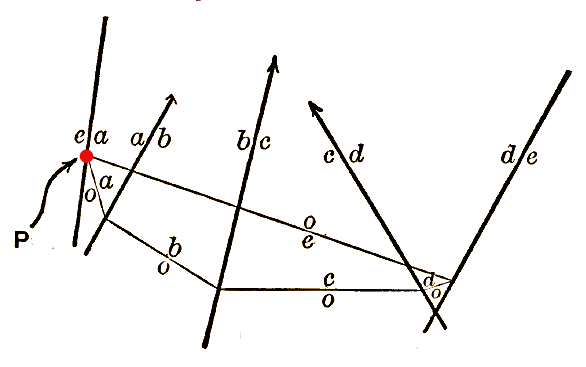
\includegraphics[width=0.55\textwidth]{pf3.png}
         }
         
         
        \subfigure[Forma Geom�trica]
           {\label{figura:fg3}
            \includegraphics[width=0.30\textwidth]{fg3.png}
           }
       }

\end{center}
\caption{Caso 3 - fonte: \citeonline{johnson1908} (editado)}
\label{figura:caso3}
\end{figure}

As for�as $AB, BC$ e $CD$ s�o totalmente conhecidas, $DE$ tem sua linha de a��o definida por $de$ e de $EA$ conhecemos apenas o ponto de aplica��o $P$ (figura \ref{figura:caso3}). Desenha-se o PF com as for�as conhecidas por inteiro, com os seus respectivos raios polares. O tra�ado das cordas  deve come�ar pelo ponto $P$, e segue pelo ponto de interse��o entre $oa$ e $ab$, at� que a linha de a��o $dc$. Para que a condi��o de equil�brio de rota��o seja atendida, a corda $oe$ deve conter o ponto de encontro entre $od$ e $de$ , bem como o ponto $P$. Tra�ando as paralelas a $oe$, partindo do polo, e $de$, pelo ponto $D$, encontra-se $E$ que fecha o PF obtendo o vetor $EA$. A linha de a��o $ea$ � determinada desenhando uma paralela � $EA$ pelo ponto $P$.



\subsection{Caso Quatro - Resolu��o de uma For�a em Tr�s Componentes}
\label{section:prob4}

No estudo das treli�as, a maior parte das linhas de a��o s�o definidas previamente pela proposta do desenho dos eixos das pe�as. A an�lise dos esfor�os pode ser feita atrav�s dos n�s (m�todo de Cremona), os pontos de uni�o dos eixos das diagonais e banzos, ou pelo m�todo das se��es, tomadas de forma a cortarem at� tr�s elementos desconhecidos da treli�a (m�todo de Culmann). Estes �ltimos s�o resolvidos pelo caso quatro, que pode ser considerado uma combina��o dos casos dois e tr�s. Uma for�a aplicada � um ponto de um corpo r�gido, tem o mesmo efeito que a aplica��o da mesma for�a em qualquer outro ponto de sua linha de a��o. Por essa afirma��o da Est�tica, pode-se considerar o ponto de interse��o entre duas das dire��es das for�as parcialmente conhecidas como o ponto $P$ e resolver o problema conforme descrito no caso tr�s. Assim feito, o vetor calculado no ponto $P$ � concorrente com as duas for�as ainda n�o completamente conhecidas, situa��o que pode ser resolvida pelo caso dois. 

\begin{figure}[!ht]
\begin{center}
  \mbox{
      \subfigure[Pol�gono de For�as]
         {\label{figura:pf4}
          \includegraphics[width=0.30\textwidth]{pf4.png}
         }
         
         
        \subfigure[Forma Geom�trica]
           {\label{figura:fg4}
            \includegraphics[width=0.50\textwidth]{fg4.png}
           }
       }

\end{center}
\caption{Caso 4 - fonte:  \citeonline{Hoskins1899}}
\label{figura:caso4}
\end{figure}

De maneira simples, imagina-se que a for�a $AB$ � a resultante das for�as conhecidas do problema, grafadas no PF e $ab$ � sua linha de a��o no FG (Figura \ref{figura:caso4}). Na forma geom�trica, encontram-se os pontos de interse��o das linhas de a��o das quatro for�as (as tr�s desconhecidas e $ab$), duas � duas. No ponto $M$ a linha de a��o da resultante das for�as conhecidas $ab$ encontra $da$ e $cd$ e $bc$ tem por $N$ seu ponto em comum. Para que as condi��es de equil�brio sejam satisfeitas, as resultantes de $bc$ e $cd$ precisam ter a mesma linha de a��o da composi��o de $ab$ e $da$ (como mesmo m�dulo e sentido contr�rio). Uma paralela � $NM$ tra�ada em $B$ representa a dire��o da composi��o de $BC$ e $CD$ e encontra a paralela � $da$ tra�ada em $A$, definindo o vetor $DA$ em m�dulo e sentido. O encontro de uma paralela � $bc$, tra�ada em $B$, com uma paralela � $cd$, pelo ponto $D$ define o ponto $C$ que fecha o PF, garantindo equil�brio de transla��o para o sistema. � importante notar que o segmento $BD$ na Figura \ref{figura:pf4} n�o representa nenhuma for�a descrita no problema, � apenas uma constru��o auxiliar para completar o desenho do PF. No sentido $DB$, � a composi��o de $DA$ e $AB$, seu inverso, $BD$ � a resultante de $BC$ e $CD$. Iguais em magnitude e dire��o, como exige a Est�tica.


\section{C�lculo das Rea��es e Esfor�os em Treli�as Planas Bi-Apoiadas}
\label{section:trelicabiGarfo}

\citeonline{malcolm2009} apontava o m�todo gr�fico como o mais conveniente para o c�lculo das ten��es em treli�as de cobertura, tanto pela velocidade, quanto pelo fato das constru��es geom�tricas fornecerem maneiras de se verificar os resultados. A Figura \ref{figura:TrExMal01} � apresentada como um exemplo ilustrativo do c�lculo das rea��es e esfor�os. Partindo do desenho dos eixos dos elementos da treli�a e conhecendo totalmente os vetores dos carregamentos, pode-se afirmar que todas as linhas de a��o das for�as no FG s�o conhecidas.

\begin{figure}[!ht]
\begin{center}
  \mbox{
      \subfigure[Treli�a - Forma Geom�trica]
         {\label{figura:TrExMal01}
          \includegraphics[width=0.50\textwidth]{TrExMal01.png}
         }
         
         
        \subfigure[Pol�gono de For�as]
           {\label{figura:TrExMal02}
            \includegraphics[width=0.45\textwidth]{TrExMal02.png}
           }
       }

\end{center}
\caption{Exemplo de C�lculo de Esfor�os de Treli�as - fonte:  \citeonline{malcolm2009}}
\label{figura:exemplotr01}
\end{figure}

\subsection{Determina��o Est�tica de Treli�as}
\label{section:determinacaoestatica}

Antes de utilizar-se um modelo matem�tico para a resolu��o de um problema, � preciso certificar-se que o modelo se aplique adequadamente ao problema. Os m�todos gr�ficos apresentados aqui lidam com problemas da Est�tica Pura. Definida como o campo da ci�ncia que trata dos problemas da Est�tica passiveis de solu��o apenas pela satisfa��o das condi��es de equil�brio dos corpos r�gidos  \cite[p. 45]{johnson1908}. Na literatura atual � mais comum encontrar os termos isost�tico e hiperest�tico apara definir os principais tipo de problema do c�lculo estrutural. Quando as equa��es de equil�brio de um corpo r�gido s�o de mesma quantidade que as vari�veis envolvidas, diz-se que o problema � isost�tico. Quando existem mais vari�veis que equa��es diz-se que o problema � hiperest�tico \cite{mccormac2009}. Para resolver um sistema estrutural hiperest�tico, s�o adicionadas equa��es ao problema, provenientes das caracter�sticas da deforma��es dos materiais de constru��o empregados (lei de Hooke). Portanto, dizer que um problema � isost�tico ou que ele pertence ao escopo da Est�tica Pura tem o mesmo significado.

A isostaticidade de uma treli�a � determinada por duas caracter�sticas e uma condi��o de igualdade. As caracter�sticas s�o:

\begin{itemize}
\item os elementos devem formar apenas tri�ngulos pelo encontro de seus eixos;
\item dois ou mais eixos devem se encontrar apenas em um n�.
\end{itemize}

A condi��o de igualdade apresentada na  Equa��o \ref{equacao:trelicaIso} \cite[p. 99]{mccormac2009} deve ser satisfeita, onde $m$ � o numero de barras (membros) da treli�a e $j$ � o n�mero de n�s.

\begin{equation}
\label{equacao:trelicaIso}
 m= (2 \times j) -3
\end{equation}

No exemplo em quest�o, nota-se por inspe��o da forma, que as duas caracter�sticas s�o satisfeitas e que existem $21$ elementos e $12$ n�s. A condi��o de igualdade ($(12 \times 2) - 3 = 21$) � atingida, portanto a treli�a � isost�tica e pode ser resolvida dentro do escopo da Est�tica Pura.

\subsection{Regras de Desenho para Obten��o de Diagramas Rec�procos}
\label{section:Sentido_select}

Antes de prosseguir com a descri��o do algoritmo de desenho, algumas regras devem ser assumidas para que as figuras geradas sejam realmente rec�procas. As propriedades que garantem a reciprocidade das figuras s�o \citeonline[p. 65]{Hoskins1899}:
\begin{itemize}
\item Para cada conjunto de linhas que se interceptam em um ponto na FG, s�o representadas no PF como um pol�gono fechado com paralelas �s respectivas linhas na outra figura.
\item A ordem das for�as representadas no PF � deve ser a mesma das linhas da FG, se observadas consecutivamente ao redor do n�.
\end{itemize}

Para que a segunda propriedade seja plenamente atingida � necess�rio estabelecer um sentido de sele��o para as for�as conhecidas e linhas de a��o que deve ser adotado tanto para o c�lculo das rea��es quanto para o dos esfor�os nas barras. O sentido adotado neste exemplo � hor�rio, o sentido anti-hor�rio poderia ser tamb�m utilizado, obtendo os mesmos valores para as inc�gnitas, desde que apenas um desses sentidos poss�veis seja utilizado em todas as etapas do processo.


\subsection{C�lculo das Rea��es}
\label{section:reacExemplo}

As rea��es de apoio $R1$ e $R2$ s�o as �nicas for�as externas desconhecidas e devem ser calculadas primeiro. Como apenas carregamentos verticais s�o aplicados � treli�a, pode-se afirmar que as duas rea��es tem dire��es tamb�m verticais. Neste caso, aplica-se o problema fundamental da Est�tica chamado de caso dois para for�as paralelas, descrito na Se��o \ref{section:prob2}. A sele��o das for�as deve seguir o sentido eleito, partindo da for�a mais pr�xima de $R1$ at� $R2$. Os raios polares e o funicular s�o desenhados (linhas pontilhadas na Figura \ref{figura:exemplotr01}) e as rea��es s�o definidas. A ordem estabelecida garante que a componente $R1$ ser� a por��o do somat�rio de for�as mais pr�xima do carregamento no n� $U1$. Analogamente ao c�lculo anal�tico, as rea��es s�o determinadas pela satisfa��o da premissa que garante o equil�brio de rota��o do sistema.

\subsection{C�lculo dos Esfor�os}
\label{section:forcasExemplo}

\begin{figure}[!h]
\begin{center}
\includegraphics[width=0.45\textwidth]{TrExMal03.png}
\caption{Pol�gono de For�as - fonte:\citeonline{malcolm2009}} 
\label{figura:PFfinalExemplo01}
\end{center}
\end{figure}

Al�m da obten��o dos m�dulos e sentidos dos esfor�os em cada elemento, do ponto de vista gr�fico, partindo dos carregamentos e resultantes calculados na Figura \ref{figura:TrExMal02}, procura-se construir um �nico pol�gono de for�as que contenha elementos rec�procos � todas as linhas de a��o da forma geom�trica, como mostrado na Figura \ref{figura:PFfinalExemplo01}. Utilizando-se do m�todo de Cremona, que procura satisfazer as condi��es de equil�brio de transla��o para cada n�, deve-se iniciar por um ponto onde no m�ximo duas for�as n�o estejam completamente determinadas. Geralmente pelos pontos de apoio, onde atuam as rea��es $R1$ e $R2$.

\begin{figure}[!h]
\begin{center}
  \mbox{
      \subfigure[N� $L0$]
         {\label{figura:TrExMalNo01}
          \includegraphics[width=0.40\textwidth]{TrExMalNo01.png}
         }
         
         
        \subfigure[N� $U1$]
           {\label{figura:TrExMalNo02}
            \includegraphics[width=0.40\textwidth]{TrExMalNo02.png}
           }
       }

\end{center}
\caption{Satisfa��o das Condi��es de Equil�brio de Transla��o - $L0$ e $U1$ - fonte:  \citeonline{malcolm2009}}
\label{figura:nosL0U1}
\end{figure}

Aplicando a condi��o de equil�brio no n� $L0$, utilizando o sentido de sele��o das for�as ao redor do ponto, deve-se ordenar os elementos atuantes de forma que as duas for�as desconhecidas sejam usadas por ultimo. Analisando o n� em quest�o, apenas a rea��o $R1$ � completamente conhecida. A partir de $R1$ no PF, desenha-se o sentido do elemento $X1$ na extremidade final e a dire��o do elemento $1Y$ no primeiro ponto, como ilustrado na Figura \ref{figura:TrExMalNo01}. Para que a condi��o de equil�brio seja completamente atendida, os vetores devem descrever um pol�gono fechado tamb�m em suas dire��es, portanto $X1$ tem sentido descendente e $1Y$ da esquerda para a direita. A defini��o da natureza dos esfor�os baseia-se nos crit�rios apresentados em \citeonline[p. 99-102]{malcolm2009}. Movendo as for�as $X1$ e $1Y$ do PF para a FG pelos seus pontos finais at� o ponto do n�, a natureza do esfor�o sera de compress�o, caso haja sobreposi��o entre os elementos do FG e o seguimento rec�proco movido do PF, como acontece com a for�a $X1$. Caso os segmentos n�o se sobreponham, como no caso da for�a $1Y$, a solicita��o � de tra��o. O procedimento de determina��o dos sentidos e natureza dos esfor�os deve ser realizado para todas as solicita��es calculadas.

Determinando todas as solicita��es que atuam em $L0$, restam apenas dois valores desconhecidos no n� $U1$. Aplicando o sentido de sele��o, partindo das for�as conhecidas procura-se os vetores $1X$ ($X1$ e $1X$ representam o mesmo elemento segundo a nota��o de Bow, que leva em conta o sentido de sele��o para determinar a nomenclatura em cada n�) e o carregamento $P$. Desenha-se as dire��es dos elementos $X2$ e $21$, partindo respectivamente do ponto final e inicial do pol�gono aberto das for�as conhecidas neste ponto. no ponto de encontro dessas duas dire��es fecha-se o pol�gono determinam os sentidos (Figura \ref{figura:TrExMalNo02}).

\begin{figure}[!h]
\begin{center}
  \mbox{
      \subfigure[N� $L1$]
         {\label{figura:TrExMalNo03}
          \includegraphics[width=0.40\textwidth]{TrExMalNo03.png}
         }
         
         
        \subfigure[N� $U2$]
           {\label{figura:TrExMalNo04}
            \includegraphics[width=0.40\textwidth]{TrExMalNo04.png}
           }
       }

\end{center}
\caption{Satisfa��o das Condi��es de Equil�brio de Transla��o - $L1$ e $U2$ - fonte:  \citeonline{malcolm2009}}
\label{figura:nosL1U2}
\end{figure} 

A determina��o completa das for�as no n� $U1$ abre caminho para resolu��o de $L1$. Pelos crit�rios de sele��o adotados, procura-se por $Y1$ e $12$ no PF (elementos completamente conhecidos) e desenha-se a dire��o de $23$ no ponto final de $12$ e $3Y$ no in�cio de $Y1$. Como $Y1$ e $3Y$ tem a mesma dire��o, ocorre uma sobreposi��o de linhas, como mostra a Figura \ref{figura:TrExMalNo03}.

A soma de vetores � uma opera��o comutativa, independem da ordem em que os vetores s�o selecionados. Obedecendo o sentido de sele��o, contudo, garante-se um �nico pol�gono de for�as para todos os n�s. Analisando $U2$ nota-se que as for�as conhecidas $32$, $2X$ e $P$ est�o grafadas no PF pelos passos anteriores, $X4$ e $43$, quando determinadas nos pontos final e inicial  respectivamente do pol�gono aberto (Figura \ref{figura:TrExMalNo04}) garantem que os v�rtices seguintes que dependem dessas for�as encontraram suas representa��es no PF nas posi��es convenientes para prosseguir com o c�lculo de um PF �nico.



\begin{figure}[!h]
\begin{center}
  \mbox{
      \subfigure[N� $L2$]
         {\label{figura:TrExMalNo05}
          \includegraphics[width=0.40\textwidth]{TrExMalNo05.png}
         }
         
         
        \subfigure[N� $U3$]
           {\label{figura:TrExMalNo06}
            \includegraphics[width=0.40\textwidth]{TrExMalNo06.png}
           }
       }

\end{center}
\caption{Satisfa��o das Condi��es de Equil�brio de Transla��o - $L2$ e $U3$ - fonte:  \citeonline{malcolm2009}}
\label{figura:nosL2U3}
\end{figure}

Em $L2$ as for�as conhecidas $Y3$ e $34$ s�o identificadas no PF e determina-se as magnitudes e sentidos desconhecidos para $45$ e $5Y$ (Figura \ref{figura:TrExMalNo05}). Em $U3$, pode-se calcular as for�as desconhecidas $x4'$ e $4'5'$ efetuando os mesmos passos a partir do v�rtice onde atua $R2$ , mas como tanto a forma da treli�a, quanto os carregamentos s�o sim�tricos em rela��o ao eixo $5'5$, os resultados para cada elemento apresentar�o mesmo m�dulo e natureza dos elementos sim�tricos j� calculados. O PF final apresentar� tamb�m simetria, como grafado na Figura \ref{figura:PFfinalExemplo01}. O c�lculo de $5'5$ � apresentado na Figura \ref{figura:TrExMalNo06} e ocorre pela aplica��o do caso um dos problemas fundamentais da Est�tica. o PF desenhado pelas demais for�as que atuam em $U3$ j� descrevem um pol�gono fechado, implicando na nulidade da magnitude de $5'5$. Optando por n�o colocar um elemento $5'5$, as condi��es de isostaticidade apresentadas na Se��o \ref{section:determinacaoestatica} ainda seriam satisfeitas com 19 elementos e 11 v�rtices ($(11 \times 2)-3=19$).

\section{C�lculo das Rea��es e Esfor�os em Treli�as Planas em Balan�o}
\label{section:trelicaBalGarfo}

\begin{figure}[!h]
\begin{center}
  \mbox{
      \subfigure[Treli�a - Forma Geom�trica]
         {\label{figura:trelicaBalancoExemplo}
          \includegraphics[width=0.55\textwidth]{trelicaBalancoExemplo.png}
         }
         
         
        \subfigure[Pol�gono de For�as]
           {\label{figura:trelicaBalancoExemploPF}
            \includegraphics[width=0.40\textwidth]{trelicaBalancoExemploPF.png}
           }
       }

\end{center}
\caption{Exemplo de C�lculo de Esfor�os de Treli�as em Balan�o- fonte:  \citeonline{malcolm2009}}
\label{figura:exemplotr02}
\end{figure}

O m�todo apresentado nesta se��o baseia-se nos algoritmos apresentados  em \citeonline[p. 145-159]{burr}, \citeonline[p. 114-116]{malcolm2009}\citeonline[p. 161-172]{goldenhorn1943} ou \citeonline[p. 132-133]{zalewski1998shaping}. Para o c�lculo das rea��es na treli�a em balan�o apresentada na Figura \ref{figura:trelicaBalancoExemplo}, deve-se primeiro analisar as rea��es $R1$ e $R2$. Enquanto a segunda tem uma dire��o definida pelo seguimento $AD$, a primeira tem dire��o desconhecida. A resolu��o usual deste problema parte do c�lculo da resultante dos carregamentos ignorando as rea��es.

Pelo caso um dos problemas fundamentais da Est�tica, a rea��o $R$ � calculada pelo fechamento do funicular. As rea��es $R1$ e $R2$ tem por soma $R$. prolongando o sentido de $R2$ at� encontrar a linha de a��o de $R$ no ponto $C$. Para satisfa��o das condi��es de equil�brio, $R1$ deve ter dire��o $BC$. Atendendo os crit�rios de sele��o e sentido (adotado o anti-hor�rio neste exemplo) em torno do ponto $R$ as rea��es s�o completamente determinadas, sendo $R1$ tra��o e $R2$ compress�o. O esfor�o no elemento $AD$ tamb�m � determinado, visto que este precisa se anular com a rea��o $R2$ em torno do n� $A$, tratam-se de for�as com mesmo m�dulo e dire��o, mas com sentidos opostos no PF. 

A resolu��o dos demais elementos da treli�a deve ser executada a partir do ponto $B$ e seguir em dire��o ao ponto $E$, respeitando os mesmos crit�rios de sele��o, sentido e constru��es geom�tricas aplicadas na resolu��o da treli�a apresentada na Se��o \ref{section:trelicabiGarfo}.

O n� $E$, entretanto, n�o chega a ser formalmente calculado, e sim serve como ferramenta de confer�ncia do C�lculo. Em torno deste n� atuam o carregamento $YX$, a solicita��o no elemento $X1$ do banzo superior e em $1Y$ no inferior. Enquanto o carregamento � um dado do problema, $1Y$ � calculado fechando o pol�gono para o n� imediatamente anterior � $E$ no banzo inferior e $X1$ para o n� imediatamente anterior � $E$ no banzo superior. Quando o elemento $X1$ � definido em magnitude � sentido, ele deve fechar os pol�gonos de for�as ao redor do ponto em que foi calculado e tamb�m em torno do ponto $E$. Se os dois pol�gonos se fecham com uma linha paralela � $X1$ na FG, o problema foi resolvido corretamente.


\section{Outros Algoritmos da Grafost�tica}
\label{section:AlgorGarfo}

Apesar das publica��es e republica��es sobre Grafost�tica terem sido drasticamente reduzidas na segunda metade do s�culo XX, a quantidade de material dispon�vel sobre o assunto � muito grande. A real dificuldade, na aus�ncia de um levantamento bibliogr�fico sobre os m�todos de solu��o para diferentes prolemas da Est�tica Gr�fica, � filtrar o material existente. Sem a pretens�o de realizar um levantamento extensivo, ser�o listados nesta se��o alguns t�picos que merecem destaque, pela clareza da exposi��o, pelo cuidado com a apresenta��o da teoria das estruturas ou por apresentarem algoritmos pouco explorados por seus pares, nos trabalhos dos autores que forneceram a fundamenta��o para o estudo da Grafost�tica realizado nesta pesquisa.

Dentre os livros t�cnicos e manuais pr�ticos consultados para a elabora��o deste trabalho (muitos deles com os direitos de publica��o e reprodu��o j� em dom�nio p�blico) encontram-se dispon�veis para consulta e \textit{download} em reposit�rios na internet (e.g. \href{http://openlibrary.org/}{openlibrary.org}), outros podem ser encontrados em territ�rio nacional, no com�rcio \textit{online} de livros usados.

Os algoritmos fundamentais, os c�lculos e diagramas de solicita��es e tens�es b�sicas para treli�as e vigas de alma cheia s�o assuntos cobertos por todas as publica��es. Destacam-se o livro de \citeonline{Hoskins1899}, pela abordagem objetiva e introdut�ria das bases da disciplina e \citeonline{johnson1908} pela cuidadosa apresenta��o dos conceitos te�ricos e o constante paralelo com os m�todos anal�ticos para os mesmos problemas. O livro de \citeonline{burr} tem um cap�tulo inteiro dedicado � teoria das linhas de influ�ncia aplicada nos algoritmos de c�lculo e an�lise, outro sobre deforma��es calculadas graficamente. \citeonline{Kneip1939} apresentam o tratamento gr�fico de eixos e gruas, com suas aplica��es ao projeto de pe�as mec�nicas. \citeonline{henkel1953} trabalha com algoritmos de deforma��o no c�lculo de equil�brio em vigas continuas. \citeonline{eddy2010new} trata de tens�es provenientes da dilata��o t�rmica e estruturas em forma de c�pula, em metal e pedra. \citeonline{malcolm2009} discute a an�lise e o c�lculo de tens�es para um s�rie de treli�as de cobertura, inclusive estruturas em balan�o e assim�tricas. \citeonline{goldenhorn1943} apresenta dois m�todos para o c�lculo de vigas continuas e o tratamento gr�fico das propriedades das se��es planas (incluindo o momento de in�rcia e o raio de gira��o). \citeonline{sanjuan1951} mostra m�todos de desenho para a determina��o gr�fica de integrais no final de seu livro, com suas aplica��es na resist�ncia dos materiais em sistemas isost�ticos e hiperest�ticos, mostrando a extens�o do poder de c�lculo desses algoritmos. \citeonline{panseri1952} trata, de maneira extensa e cuidadosa com os aspectos te�ricos da F�sica, as propriedades de se��es planas, apresentando os m�todos de Culmann e Mohr para o c�lculo destas propriedades. As aplica��es das derivadas e integrais gr�ficas no tratamento dos esfor�os cortante e momento fletor abordadas pelo autor, tamb�m merecem destaque. \citeonline{Bayle1966} apresenta objetivamente os aspectos b�sicos da Grafost�tica com a particularidade de, ao final de cada cap�tulo, mostrar de maneira resumida as correlatas aplica��es anal�ticas e m�todos de verifica��o do c�lculo gr�fico pela utiliza��o de express�es matem�ticas. O trabalho te�rico de \citeonline{Crapo} � considerado fundamental \cite{gerhardt2003} \cite{aag2010193} para a formula��o do estudo tridimensional da Grafost�tica. O livro de \citeonline{zalewski1998shaping} � uma publica��o recente sobre o tema, largamente ilustrada onde a Est�tica Gr�fica � utilizada como ferramenta para a cria��o e refino de forma, demonstra o renovado interesse de institui��es respeitadas de ensino e pesquisa como o MIT e a Universidade de Yale a respeito do m�todo. A �nica publica��o nacional encontrada nesta pesquisa foi a de \citeonline[p. 3-39]{costa1974} que, apesar de utilizar a Grafost�tica com recurso introdut�rio para o estudo anal�tico de Resist�ncia dos Materiais, apresenta em poucas p�ginas os fundamentos b�sicos da disciplina de maneira clara e objetiva.




\section{Ferramentas Computacionais}
\label{section:ferramentascomputacionais}

\begin{itemize}

\item \textbf{ActiveStatics:} Desenvolvido por Simon Greenwold no MIT (\citeauthor{GREENWOLD}), � considerada a primeira implementa��o computacional baseada em Grafost�tica. Idealizada como ferramenta de ensino, o programa implementa alguns algoritmos gr�ficos de Est�tica que podem ser dinamicamente experimentados \cite{Shearer2010};

\item \textit{\textbf{eQUILIBRIUM:}} Implementa��o na plataforma educacional \textit{Open sourse} GeoGebra de alguns m�todos da Est�tica Gr�fica pelo \citeauthor{BLOCKResearchGroup} da Polit�cnica de Zurique;

\item \textbf{CADenary:} Uma ferramenta baseada em Grafost�tica implementada na linguagem de \textit{scripts} \textit{Processing} (\citeauthor{Kilian});

\item \textbf{RhinoStatics:} Desenvolvido como parte da disserta��o de mestrado de \citeonline{Shearer2010}, ferramentas Grafost�ticas s�o desenvolvidas sobre a forma de \textit{scripts}, em linguagem \textit{Visual Basic} no ambiente \textit{Rhinoceros}. As solu��es s�o constru�das atrav�s de fun��es que manipulam entidades gr�ficas. Qualquer altera��o feita nas geometrias, porem, deve ser redesenhada por novas chamadas das fun��es do programa;

\item Os algoritmos propostos por \citeonline{lachauer2011a}, a �nica ferramente computacional baseada em Grafost�tica, implementada em um ambiente altamente din�mico como o \textit{Grasshopper}, que esta pesquisa encontrou. Aplicados como modelo de an�lise e gera��o \textit{form finding}, os algoritmos s�o propostos em um ambiente (\textit{Rhinoceros, Grasshopper, VB.net}) semelhante ao utilizado neste experimento (\textit{Rhinoceros, Grasshopper, Python}).

\end{itemize}


    % !TeX encoding = ISO-8859-1
% !TeX spellcheck = pt_BR
\chapter{Ambiente de Implementa��o}\label{chapter:ambientedeimplementacao}


\begin{flushright}
\textit{"If you want to teach people a new way of thinking, \\don't bother trying to teach them.\\ Instead, give them a tool, the use of which\\ will lead to new ways of thinking."} \\ (R. Buckminster Fuller)
\end{flushright}

A ideia de aproximar a programa��o de formas e an�lises � atividade de projeto vem ganhando for�a e espa�o, principalmente nos grandes escrit�rios de arquitetura ao redor do mundo. O \textit{"Specialist Modeling Group"} do escrit�rio \textit{Foster and Partners'} ou o \textit{"CODE unit"} de \textit{Zaha Hadid Architects} s�o exemplos de departamentos de programa��o, criados em firmas de arquitetura para trabalhar em coopera��o e sincronia com os demais setores, na elabora��o de propostas e projetos \cite{ceccato2010mbg}.

\begin{figure}[!ht]
\begin{center}
  \mbox{
      \subfigure[Interface do \textit{Rhinoceros 3D} 5.0 ]
         {\label{figura:rhinoInterface}
          \includegraphics[width=0.45\textwidth]{rhinoInterface.jpg}
         }
         
         
        \subfigure[Interface do \textit{Grasshopper} e \textit{Rhinoceros 3D} 5.0 ]
           {\label{figura:rhinoGrassInterface}
            \includegraphics[width=0.45\textwidth]{rhinoGrassInterface.png}
           }
       }
        
  \mbox{
        \subfigure[Interface do \textit{GH.Python}]
                   {\label{figura:interfaceghpython}
                    \includegraphics[width=0.45\textwidth]{interfaceghpython.png}
                   }
       }

\end{center}
\caption{Ambiente de Implementa��o}
\label{figura:ambienteimplem}
\end{figure}


As demandas de programa��o entretanto, devem se adaptar aos cronogramas e prazos da atividade fim. Por isso, as linguagens de c�digo e \textit{scripts} devem ter f�cil intera��o com os ambientes computacionais de projeto, permitindo trabalho r�pido, eficiente, manipula��o de entidades gr�ficas vetoriais e reaproveitamento de algoritmos em diferentes atividades.


Dentre os muitos poss�veis sistemas \textbf{CAD} que poderiam ser utilizados para a implementa��o do experimento, foi escolhido o \textit{Rhinoceros 3D} 5.0 e o  \textit{plug-in} \textit{Grasshopper}, com �nfase no ambiente de  \textit{Python Script} suportado por ambos (Figura \ref{figura:ambienteimplem}).

\section{\textit{Rhinoceros 3D}}
\label{section:rhinoceros3d}

O \textit{Rhinoceros 3D} , assim como o \textit{Autodesk Autocad}, \textit{BricsCAD}, \textit{LibreCAD}, entre outros,  � um \textbf{CAD} de interface baseada em linha de comando (marcada com a letra "A" na figura \ref{figura:rhinoInterface}). Com caracter�sticas mais adaptadas � modelagem 3D, principalmente de curvas e superf�cies complexas, � usado em diversos ramos do \textit{design} industrial e foi adotado pelo mercado de arquitetura \cite{ceccato2010mbg}, desempenhado papeis importantes nas etapas iniciais de concep��o de projeto. Um dos motivos que levaram � esse uso est� no fato do programa ser constru�do como um conjunto de bibliotecas gr�ficas envoltas por uma interface CAD, potencializada por \textit{plug-ins}. A principal dessas bibliotecas � a \textit{OpenNurbs}, desenvolvida e mantida pela empresa respons�vel pelo \textit{Rhinoceros} e \textit{Grasshopper} (\textit{Robert McNeel \& Associates}) porem com licen�a \textit{open source}, nela est�o os m�todos de grava��o e leitura dos arquivos .3dm e a representa��o das formas geom�tricas do programa. O desenvolvimento de novas funcionalidades do \textit{software} s�o feitas atrav�s de \textit{plug-ins}, usado o mesmo IDE dispon�vel para programadores terceiros, as fun��es e m�todos de grava��o e manipula��o de entidades gr�ficas podem ser acessadas tanto em C++, a linguagem de programa��o em que o programa � escrito, quanto em linguagens interpretadas (\textit{C\#, VB.net }e \textit{Python}) que permitem mais r�pida cria��o e manipula��o de algoritmos \cite{Tibbits2011}.

Essas caracter�sticas atra�ram tamb�m o interesse de trabalhos acad�micos e pesquisas, que usam a plataforma para implementa��o e testes de seus algoritmos. \cite{Tessmann2008},  \cite{Block2009}, \cite{vettoretti2010}, \cite{Shearer2010}, \cite{1148846}, \cite{lachauer2011a},  \cite{dalvi2011}, \cite{Block2014}.




\section{\textit{Grasshopper}}
\label{section:grasshopper}

Um dos \textit{plug-ins} desenvolvido pela \textit{Robert McNeel \& Associates} para expans�o das capacidades do \textit{Rhinoceros 3D} � o \textit{Grasshopper}, uma interface visual de programa��o e cria��o de modelos param�tricos \cite{lachauer2011a}. A interface do \textit{plug-in}, mostrada na Figura \ref{figura:rhinoGrassInterface}, permite a elabora��o de algoritmos pela interliga��o de componentes, tamb�m chamados de baterias (\textit{batteries}), que desempenham papeis de armazenamento de informa��es (vari�veis e objetos), ou de fun��es que manipulam objetos geom�tricos. Existem tr�s aspectos importantes da integra��o entre programa e \textit{plug-in} que precisam ser entendidos:

\begin{itemize}
\item \textbf{Comunica��o \textit{Rhinoceros/Grasshopper}}: todas as geometrias desenhadas no \textit{Rhinoceros}, pontos, curvas, superf�cies, s�lidos e combina��es de elementos, podem ser selecionados a partir de um componente do \textit{Grasshopper}, usadas como vari�veis ou objetos, e manipuladas pelos componentes seguintes do algoritmo proposto.
\item \textbf{Ambiente de Modelagem do \textit{Grasshopper}}: todas as formas geradas pelos algoritmos do \textit{Grasshopper} s�o, por padr�o, mostradas na janela no \textit{Rhinoceros}, mas apenas os elementos desenhados no \textit{Rhinoceros} podem ser editadas por este. As geometrias criadas pelo algoritmo s�o dinamicamente alteradas pela edi��o de uma geometria selecionada em uma bateria do \textit{plug-in}, ou pela altera��o de qualquer elemento do algoritmo. Essa velocidade de gera��o das varia��es � que torna o sistema interessante como ferramenta para avalia��o de alternativas de projeto.
\item \textbf{Comunica��o \textit{Grasshopper/Rhinoceros}}: qualquer geometria gerada pelos componentes do \textit{Grasshopper} pode ser copiada, em uma configura��o espec�fica dos par�metros que a geraram, como uma geometria do \textit{Rhinoceros}, podendo ent�o, ser editada como qualquer outra.
\end{itemize}



\begin{figure}[!ht]
\begin{center}
  \mbox{
      \subfigure[Exemplo 1 - \textit{Grasshopper}]
         {\label{figura:grassExgh1}
          \includegraphics[width=0.45\textwidth]{grassExgh1.png}
         }
         
         
        \subfigure[Exemplo 1 - \textit{Rhinoceros 3D}]
           {\label{figura:grassExrs1}
            \includegraphics[width=0.45\textwidth]{grassExrs1.png}
           }
       }
        
  \mbox{
        \subfigure[Exemplo 2 - \textit{Grasshopper}]
           {\label{figura:grassExgh2}
            \includegraphics[width=0.45\textwidth]{grassExgh2.png}
           }
           
           
          \subfigure[Exemplo 2 - \textit{Rhinoceros 3D}]
             {\label{figura:grassExrs2}
              \includegraphics[width=0.45\textwidth]{grassExrs2.png}
             }
         }

\end{center}
\caption{Grasshopper - Componentes e listas }
\label{figura:ghexemplos}
\end{figure}


Outro conceito importante � que a grande maioria das entradas e sa�das dos componentes s�o tratados como listas numeradas. Cada elementos de uma lista com $N$ valores recebe uma numera��o, chamada de �ndice, partindo de zero at� $N - 1$. A Figura \ref{figura:ghexemplos} mostra o mesmo algoritmo com apenas uma reta armazenada no componente \textit{"Crv"} (Figura \ref{figura:grassExgh1}) e com duas curvas selecionadas no mesmo componente (Figura \ref{figura:grassExgh2}), bem como as respectivas geometrias resultantes (Figuras \ref{figura:grassExrs1} e \ref{figura:grassExrs2}). A organiza��o padr�o dos componentes do \textit{Grasshopper} � que as entradas e sa�das s�o feitas pela "conex�o de fios" no sentido esquerda-direita. Nos exemplos da Figura \ref{figura:ghexemplos}, o componente \textit{"Divide"} recebe como entrada a(s)  curva(s) do componente \textit{"Crv"} (segmentos de retas desenhadas no \textit{Rhinoceros}, selecionadas e armazenadas) e um valor inteiro no componente \textit{"Count"}. Os segmentos selecionados em "Crv" s�o lidos pela entrada $C$ do componente \textit{"Divide"} e s�o divididos em $N$ partes iguais, tendo o n�mero inteiro fornecido por \textit{"Count"} como a quantidade de partes. Se na esquerda do componente \textit{"Divide"} se conectam as listas de entrada, na direita s�o lidas as sa�das. No exemplo em quest�o, apenas a saida $P$, com lista(s) de pontos que dividem o(s) seguimento(s), � usada. Os componentes \textit{"Count"}, "h pilastas" e \textit{"Radius"} s�o chamados de \textit{sliders}, pois o valor num�rico passado por estes pode ser alterado deslizando o elemento gr�fico que marca sua posi��o. enquanto o primeiro desses � uma vari�vel inteira, os outros s�o n�meros reais que controlam respectivamente a altura dos elementos cil�ndricos e seu raio. Uma diferen�a vis�vel entre o mesmo algoritmo nas Figuras \ref{figura:grassExrs1} e \ref{figura:grassExrs2} � a maneira como os "fios" que conectam as baterias s�o representados. Na primeira vemos uma linha simples ligando \textit{"Crv"} � \textit{"Divide"} representando que apenas um elemento (ou uma lista unit�ria) � passado como entrada para o componente, na sa�da $P$ uma linha dupla indica que uma lista com $N+1$ pontos (os pontos que dividem o segmento em $N$ partes contando com os extremos deste). Na segunda, uma linha dupla indica que mais de um elemento est�o armazenados em "Crv", gerando duas listas numeradas (uma para cada conjunto de $N+1$ pontos que dividem os segmentos) na saida $P$, neste caso, a primeira curva selecionada recebe o �ndice zero (0), e a segunda � numerada como um (1). As linhas duplas e tracejadas que saem de $P$ no segundo exemplo s�o usadas para indicar que um conjunto de listas numeradas (\textit{Data Tree}) est� sendo transmitido entra as sa�das e entradas das respectivas baterias.

O componente \textit{"Move"} recebe a(s) Lista(s) de pontos e um vetor para move-los oriundo da combina��o do \textit{slider} "h pilastras" com um vetor unit�rio na dire��o "Z". Cada elemento da lista $P$ � movido em m�dulo, dire��o e sentido do vetor e a sa�da $G$ � preenchida com lista(s) cuja numera��o corresponde aos respectivos �ndices dos elementos � serem movidos na entrada $G$ . A bateria "Ln" cria segmentos de reta (pares ordenados de pontos) entre os valores recebidos pelas entradas $A$ e $B$, segundo a ordem dos �ndices de cada elemento. A bateria \textit{"Pipe"}, por fim, cria as geometrias equivalentes � transla��o de um c�rculo, cujo raio � definido pela entrada $R$, ao londo da(s) curva(s) que alimentam a entrada $C$.

A vantagem do sistema descrito � que a simples altera��o do valor de um \textit{slider} ou a edi��o e/ou substitui��o de um objeto geom�trico selecionado � imediatamente reprocessada pelo \textit{constraint solver} que calula as geometrias no \textit{plug-in}, proporcionando uma r�pida visualiza��o das alternativas de projeto. L�gicas semelhantes podem ser encontradas no editor param�trico de texturas do \textit{Software Maya 3D} ou na modelagem param�trica do pacote de efeitos especiais para o cinema Houdini. Na �rea de arquitetura, o \textit{plug-in} \textit{Dinamo}, para \textit{Revit} e \textit{Vassari}, apresenta interface e l�gica semelhantes ao \textit{Grasshopper}. As ferramentas de cria��o de algoritmos do \textit{plug-in} se aproximam dos paradigmas que originaram a linguagem de programa��o Lisp, presentes no artigo cl�ssico de \citeonline{McCarthy1960}, no que tange as listas e no aspecto n�o destrutivo desta manipula��o (no exemplo da Figura \ref{figura:ghexemplos}, v�-se que os pontos transformados pelo componente \textit{"Move"} n�o destroem a lista de pontos que serve de entrada), se afastam porem, no que diz respeito ao conceito de recursividade (uma das formas de se criar um \textit{loop} em programa��o). O paradigma Lisp � frenquentemente associado � criatividade na programa��o. \citeonline{Steele:1996:EL:234286.1057818} relacionam este fato ao perfil dos usu�rios da linguagem (bastante aplicada � �rea de inteligencia artificial). De maneira otimista, pode-se esperar que criatividade tamb�m apare�a na manipula��o de listas por profissionais de projeto.

N�o existe uma maneira de se implementar um \textit{loop} com os componentes do pacote b�sico do \textit{Grasshopper}. O componente \textit{Hoopsnake}, desenvolvido por \citeonline{hoopsnake} e instalado como um \textit{Add-on}, foi usado nos exemplos apresentados no Ap�ndice \ref{figura:tsAg2d} para submeter �s transforma��es geom�tricas � um \textit{loop} semelhante ao \textit{For} com um contador como crit�rio de parada. A manipula��o de listas � a principal ferramenta l�gica de programa��o do \textit{plug-in}. No Ap�ndice \ref{Apend1:somavetconcorre}
temos um teste feito com os componentes padr�o do \textit{Grasshopper}, modelando a soma de vetores e o c�lculo da equilibrante. O recurso encontrado para a coloca��o dos vetores em posi��o de soma foi:

\begin{enumerate}
\item Criar uma lista de segmentos de reta que ligam os vetores com o ponto de coordenadas 0,0,0;
\item Mover os vetores tendo como par�metro as respectivas linhas que o ligam � origem do espa�o cartesiano;
\item Extrair uma lista dos extremos finais dos vetores movidos. Os valores de x,y,z nestes extremos, correspondem �s componentes dos respectivos vetores decompostos nas 3 dire��es;
\item O ponto inicial do PF � acrescentado no in�cio da lista de extremos. O ponto final da mesma lista � retirado;
\item Um componente de soma em massa � utilizado. Ele recebe a lista gerada no passo anterior e retorna uma lista contendo: no �ndice zero, o valor do �ndice zero da lista original; no �ndice um a soma dos valores de �ndices zero e um; e assim sucessivamente, at� que no �ndice $N$ temos a soma dos $N$ valores na lista inicial.
\item Os vetores s�o movidos a partir do seu ponto inicial, at� cada um dos pontos da lista obtida no passo anterior.
\end{enumerate}

Apesar do interessante desafio l�gico de se estabelecer um algoritmo contando unicamente com manipula��es de listas, sem utilizar explicitamente um \textit{Loop}, do ponto de vista pr�tico � bastante trabalhoso. Portanto, uma linguagem de \textit{script} foi escolhida para integrar o processo. 



\section{\textit{Python Script}}
\label{section:ghPython}

\textit{Python} � uma linguagem de programa��o \textit{open source}, interpretada, altamente din�mica, multi-paradigma e multi-plataforma, implementada por Guido van Rossum a partir de 1989 e desenvolvida pela funda��o sem fins lucrativos chamada de \textit{The Python Software Foundation}. Possui sintaxe simples e din�mica, proporcionando f�cil implementa��o, manuten��o e adapta��o de c�digos. Plenamente adaptada as bibliotecas do \textit{OpenNurbs, Rhinoceros e Grasshopper}, o aspecto multi-paradigma da linguagem � um diferencial do \textit{Python} em rela��o �s outras linguagens \textit{script} dispon�veis. Pode-se dizer, em suma, que tanto \textit{loops} semelhantes aos encontrados em linguagens como $C$ e manipula��o de listas semelhantes �s do paradigma Lisp, podem ser facilmente implementados em \textit{Python} \cite{ThepythonFoundation}.


    % !TeX encoding = ISO-8859-1
% !TeX spellcheck = pt_BR
\chapter{Trabalho experimental e desenvolvimento da pesquisa}
\label{chapter:trabalhoexperimental}


\begin{flushright}
  "\textit{With four parameters I can fit an elephant,\\
  and with five I can make him wiggle his trunk.}"
  \\(John von Neumann)
\end{flushright}

Analisando o experimento, levando-se em conta as potencialidades e limita��es do ambiente de implementa��o e imaginando uma estrat�gia de trabalho, optou-se pela subdivis�o do problema em tr�s algoritmos interconectados. A Figura \ref{figura:fluxograma_geral_01} mostra como esses algoritmos relacionam-se, e como o projetista interage e manipula os par�metros e regras para explorar as poss�veis solu��es do problema. Tendo por base o fluxograma apresentado na Figura \ref{figura:fluxogramametodologia}, restringindo-se porem as rela��es entre os algoritmos e o usu�rio.

\begin{figure}[!ht]
\begin{center}
\includegraphics[width=0.55\textwidth]{fluxograma_geral_01.jpg}
\caption{Fluxograma Geral do Experimento}
\label{figura:fluxograma_geral_01}
\end{center}
\end{figure}

Comparando com o modelo te�rico, mostrado na Figura \ref{figura:mod}, os componentes "Algoritmos de Gera��o dos Eixos" e "Algoritimo de Gera��o da Volumetria" controlam as "flex�es poss�veis do modelo geom�trico"; o "Algoritmo de An�lise Grafost�tica" corresponde � "Grafost�tica", marcada na �rea de interse��o entre a F�sica e a Geometria no modelo te�rico; ao "Projetista" cabe escolher a forma final de projeto uma otimiza��o hibrida de objetivos quantitativos e qualitativos.

\begin{figure}[!ht]
\begin{center}
\includegraphics[width=0.95\textwidth]{algGeral.png}
\caption{Captura de tela dos componentes onde os algoritmos foram implementados}
\label{figura:algGeral}
\end{center}
\end{figure}

As formas geradas pelo "Algoritmo de Gera��o dos Eixos" s�o usadas, junto com outros par�metros, tanto para a gera��o da volumetria, quanto para a an�lise da estrutura. O "Algoritimo de Gera��o da Volumetria" � lido junto com a forma dos eixos pelo "Algoritmo de An�lise Grafost�tica" e o conjunto dos resultados � avaliado pelo projetista para que decis�es sejam tomadas. Nesta cap�tulo ser�o apresentados cada um dos algoritmos que comp�em o experimento, bem como sua atua��o em conjunto, valida��o e uma an�lise dos resultados obtidos.

\section{Divis�o da Treli�a em Elementos e Nomenclatura Utilizada}
\label{section:Nomenclaturadaviga}

As treli�as desenhadas pelos Algoritmos s�o subdivididas em elementos para manipula��o e estudo. Na figura \ref{figura:Nomenclaturadaviga}(esq.)  vemos  a nomenclatura padr�o dos elementos de uma treli�a. Os elementos no limite superior e inferior das vigas s�o chamados de banzos. os elementos internos s�o chamados e diagonais.

\begin{figure}[!ht]
\begin{center}
\includegraphics[width=0.95\textwidth]{trelicanomenclatura.jpg}
\caption{Fluxograma Geral do Experimento}
\label{figura:Nomenclaturadaviga}
\end{center}
\end{figure}

A mesma solu��o � desenhada na Figura \ref{figura:Nomenclaturadaviga}(dir.) com os seus elementos separados em 4 grupos para melhor entendimento, juntamente com a nomenclatura proposta. A treli�a foi dividida em tr�s vigas e um elemento de liga��o entre estas, denominado de Conector. Este �ltimo, ao centro, liga as tr�s vigas geradas e possui cinco elementos, quatro deles de borda, formando um quadril�tero, e um central sempre na orienta��o vertical, chamado de eixo do conector. Os pontos do conector de mesma coordenada $x$ s�o referidos como $ptX1$ (superior)  e $ptX2$ (inferior), e os de mesma coordenada $y$ foram chamados de $ptY1$ (coincidindo com o �ltimo n� do banzo superior de v1) e $ptY2$ (coincidindo com o �ltimo n� do banzo superior de v2). A viga "v3", tamb�m chamada de "viga do shed", suporta a cobertura que protege a abertura de ventila��o e ilumina��o.  As vigas "v1" e "v2" s�o constru�das a partir de curvas sim�tricas em rela��o ao eixo do conector. A simetria porem, so � completa se ambas apresentarem o mesmo n�mero de diagonais e a mesma altura na por��o pr�xima aos respectivos apoios, informa��es definidas entre os par�metros de entrada do algoritmo de gera��o dos eixos. Nas tr�s vigas s�o mostrados os elementos dos banzos e diagonais, de acordo com a ordem com que s�o numerados, assim como os n�s.

Para os banzos superiores foi adotado a nomenclatura $bs$ seguida do n�mero, em sequ�ncia que parte do elemento mais pr�ximo ao apoio, nos casos das vigas "v1" e "v2", e mais pr�ximos no conector, no caso da viga "v3". A numera��o vai de 0 (zero) at� n-1 (sendo n o n�mero de elementos do banzo superior de cada viga). Por fim, o nome de cada viga � acrescentado separado pelo caractere \textit{underscore}. Para os elementos do banzo superior da viga "v1" tem-se a sequ�ncia: bs0\_v1, bs1\_v1 ... bs(n-1)\_v1.

Para as diagonais e banzos inferiores substitui-se o prefixo "bs" por "dg" e "bi", mantendo os mesmos crit�rios para o restante da nomenclatura. Para o banzo inferior tem-se :  bi0\_v1, bi1\_v1 ... bi(n-1)\_v1. Pra as diagonais :  dg0\_v1, dg1\_v1 ... dg(n-1)\_v1.

Os n�s s�o nomeados de forma semelhante aos elementos, acrescentando um "n" no prefixo:
nbs0\_v1, nbs1\_v1 ... nbs(n)\_v1. Cada n� pode ser nomeado de duas maneiras, uma em rela��o ao banzo a que pertence e outra em refer�ncia a diagonal. Os n�s do conector tamb�m coincidem com n�s das vigas.



\section{Algoritmo de Gera��o dos Eixos}
\label{section:AlgorEixos}

A modelagem de estruturas atrav�s dos eixos dos componentes � utilizada pela grande maioria dos m�todos de c�lculo e tamb�m pelas mais comuns estrat�gias de detalhamento e constru��o. O primeiro componente deste trabalho tem por principal fun��o o desenho dos eixos dos componentes da treli�a, mas tamb�m tra�a os eixos da cobertura, levando em conta a abertura do shed, e testa a determina��o Est�tica da treli�a gerada.

\begin{figure}[!ht]
\begin{center}
      \subfigure[Eixos Gerados pelo Componente - \textit{Rhinoceros}]
         {\label{figura:eixos_01_rhino}
          \includegraphics[width=.70\textwidth]{eixos_01_rhino.jpg}
         }

        \subfigure[Componente de Gera��o dos Eixos - \textit{Grasshopper} ]
           {\label{figura:eixos_01_grass}
            \includegraphics[width=.70\textwidth]{eixos_01_grass.jpg}
           }
\end{center}
\caption{Algoritmo de Gera��o dos Eixos}
\label{figura:eixos_01}
\end{figure}


Na Figura \ref{figura:eixos_01_rhino} vemos uma solu��o gerada pelo algoritmo com as vari�veis ajustadas como mostrado na Figura \ref{figura:eixos_01_grass}. As onze entradas (\textit{inputs}) do algoritmo e as implica��es destas na forma gerada ser�o comentadas em seguida.


\subsection{Par�metro 1: Curva}
\label{subsection:paramCurva}

O primeiro par�metro (Figura \ref{figura:eixos_01_grass}) de cima para baixo), denominado "Curva", � um dos par�metros obrigat�rios do algoritmo, e de crucial import�ncia para o experimento. Na Figura \ref{figura:eixos_01_rhino}, v�-se um objeto descrito com o texto "Selecionado na entrada Curva". Inicia-se o trabalho desenhando uma curva no ambiente do \textit{Rhinoceros}, selecionando no componente "Crv"(Figura \ref{figura:eixos_01_grass}) que alimenta a entrada "Curva" do algoritmo.

A curva define o formato dos banzos superiores da treli�a. Para melhor visualiza��o e manipula��o, optou-se por mover o desenho dos eixos 10 unidades acima da curva selecionada. Isso pode ser visto na Figura \ref{figura:eixos_01_rhino}, onde a curva inicial est� nomeada como 'Selecionado na entrada "Curva"'. Na citada figura, al�m de ser movida em 10 unidades, a curva inicial est� sendo reduzida por um fator de escala definido pelo par�metro "VigaDist". 

O par�metro aceita tanto curvas \textit{nurbs} (\textit{Non Uniform Rational Basis Spline}); quanto polilinhas, formadas por seguimentos retos e policurvas, que podem ser geradas a partir da uni�o de arcos, curvas e retas. Uma restri��o importante � quanto ao sentido de grafia da curva. Em um sistema CAD as linhas e curvas s�o armazenadas na ordem em que os pontos s�o inseridos. Para o correto funcionamento dos algoritmos, o sentido da curva deve partir do ponto inicial do banzo superior da viga "v1" e segui na dire��o do ponto final do banzo superior da viga "v3". No \textit{Rhinoceros} o sentido da curva pode ser visualizado pelo comando \textit{direction} e invertido pela op��o \textit{flip} do mesmo comando.

Esta curva � a principal liga��o do m�todo de trabalho proposto com as pr�ticas de projeto tradicionais, e tem efeito predominante sobre o aspecto est�tico da treli�a. A curva pode ser desenhada diretamente no \textit{Rhinoceros}, criada a partir da jun��o de segmentos, ou rascunhada em papel e digitalizada, seguindo a metodologia preferida do projetista.

Um \textit{offset} (denomina��o de comando ou fun��o existente em diversas plataformas CAD, que realiza uma c�pia paralela de uma reta ou curva � uma certa dist�ncia) a 0.2 unidades da curva � gerado e nomeado como $Cob1$, representando o eixo da cobertura sobre as vigas "v1" e "v3".

\subsection{Par�metro 2: Eixo de Simetria}
\label{subsection:paramEixosim}

O segundo par�metro opera diretamente sobre o par�metro anterior. Sua fun��o � definir o ponto $ptX1$, coincidente com o ponto inicial do banzo superior da viga "v3" e que � o primeiro ponto do eixo de simetria $ptX1 - ptX2$ e determina, n�o s� o eixo do conector, mas tamb�m o eixo de simetria entre as curvas guias dos banzos superiores das vigas "v1" e "v2".

O par�metro pode receber dois tipos de entrada : um n�mero real entre 0 e 1, ou uma reta. No primeiro caso o ponto $ptX1$ � definido pela propor��o $L \times p$ onde $L$ � o comprimento total da curva inicial e $p$ o valor num�rico entre 0 e 1. No segundo caso, para permitir a sele��o de um ponto espec�fico e preciso sobre a curva inicial, o ponto � determinado pela intersec��o de uma reta com a curva inicial. Neste caso, a reta e a curva inicial precisam estar no mesmo plano.

\subsection{Par�metro 3: HV1}
\label{subsection:paramHV1}

O terceiro par�metro representa a medida do segmento $ptX1 \quad ptX2$. Recebe um valor real positivo. O ponto $ptX2$ � gerado pela c�pia no sentido $-y$ do plano de desenho � uma dist�ncia correspondente ao valor do par�metro "HV1", e uma linha � tra�ada entre os pontos. Esta linha representa um elemento do conector, e tamb�m o eixo em que a curva inicial � dividida em duas, uma que serve de guia para o banzo superior da viga "v1", outro como guia do banzo superior de "v3". A primeira parte � espelhada em rela��o ao eixo do conector gerando assim a linha guia do banzo superior de "v2".

As curvas guias descritas acima fazem parte das "geometrias ocultas" usadas pelo algoritmo para a gera��o das formas finais, e ser�o denominadas como $gs\_v1$, $gs\_v3$ e $gs\_v2$ respectivamente. O termo "geometrias ocultas" aqui empregado refere-se a uma s�rie de objetos geom�tricos que s�o gerados pelo algoritmo, e representam est�gios intermedi�rios da s�rie de passos que, ao seu final, apresentar�o as geometrias que o processo tem por objetivo. Apenas as formas geom�tricas endere�adas � uma das sa�das do componente s�o visualizadas pelo usu�rio.

Um offset da curva $gs\_v2$ � 0.2 unidades � gerado e denominado como $Cob2$, representando o eixo da cobertura sobre a viga "v2". Antes de ser endere�ada para a sa�da "Cobertura", a curva $Cob2$ � editada conforme descrito na Se��o \ref{subsection:paramNoshed}.

Duas geometrias ocultas s�o geradas ap�s a defini��o do ponto $ptX2$. As dist�ncias entre o ponto $ptX2$ e as curvas $gs\_v1$ e $gs\_v2$ s�o calculadas e um \textit{Offset} de cada uma das curvas ($gs\_v1$ e $gs\_v2$) � criado de acordo com as dist�ncias encontradas, respectivamente referidas como $gi1\_v1$ e $gi1\_v2$, e seccionadas no ponto $ptX2$. As curvas $gs\_v1$ e $gs\_v2$ tamb�m s�o seccionadas, tendo o ponto sobre a corva mais pr�ximo de $ptX2$ como ponto de corte. Esses pontos tamb�m s�o utilizados para o desenho das bordas do conector, o ponto sobre a curva $gs\_v1$ � o ponto $ptX1$, e o ponto sobre $gs\_v2$ � $ptX2$.

Ligam-se os pontos $ptX1$, $ptY1$, $ptX2$ , $ptY2$ e fecha-se o quadril�tero no ponto inicial $ptX1$ com uma polilinha, gerando assim as bordas do conector.

Um \textit{offset} da curva $gs\_v3$ � gerado, na dist�ncia ela e o ponto $ptY2$, denominada de $gi\_v3$. 


\subsection{Par�metros 5 e 7: HV2 e HV3}
\label{subsection:paramHV2HV3}

O par�metro HV2 recebe um valor real maior que zero, representando a altura da viga "v1" no extremo do apoio.

O par�metro HV3 recebe um valor real maior que zero, representando a altura da viga "v2" no extremo do apoio.

A altura no extremo do apoio � controlada atrav�s das curvas auxiliares $gi2\_v1$, para a viga v1, e $gi2\_v2$ em v2. Os banzos inferiores das vigas v1 e v2 s�o determinados com o auxilio de duas curvas guias cada. Assim como a curva guia $gi1\_v1$ (cuja cria��o � comentada na Se��o \ref{subsection:paramHV1}), a curva $gi2\_v1$ � gerada por um \textit{offset} da curva guia do banzo superior, $gs\_v1$, a uma dist�ncia correspondente ao valor do par�metro HV2. O mesmo vale para as curvas $gi1\_v2$ e $gi1\_v2$, gerados a partir da curva $gs\_v2$ tendo como dist�ncia o par�metro HV3, na viga v2. 

Os par�metros HV2 e HV3 s�o opcionais, caso nenhum valor seja recebido por uma das entradas citadas, o valor de HV1 � usado, for�ando uma viga de altura constante entre o apoio e o conector. A maneira como as linhas guias s�o usadas para o desenho das treli�as esta descrito na Se��o \ref{subsection:funcV1V2}.

\subsection{Par�metros 4, 6 e 8: diagV1, diagV2 e diagV3}
\label{subsection:paramdiagV1diagV2diagV3}

Os par�metros diagV1, diagV2 e diagV3 definem respectivamente o n�mero de diagonais das vigas "v1", "v2" e "v3". As entradas diagV2 e diagV3 s�o opcionais, caso n�o recebam valor  diagV2 assume o mesmo valor de diagV1 e diagV3 � carregado com o valor nove.


\subsection{Par�metro 9: No\_Shed}
\label{subsection:paramNoshed}

Determina em que n� da viga "v2" termina a cobertura sobre esta, e come�a a abertura de ilumina��o e ventila��o do \textit{Shed}. Recebe um valor inteiro e maior que zero. O n�mero recebido pelo par�metro corresponde ao ultimo n� do banzo superio de "v2" � servir de apoio para a cobertura, contado no sentido inverso, ou seja, partindo do n� mais pr�ximo do conector, em dire��o ao mais pr�ximo do apoio, no citado banzo. A curva $Cob2$ � cortada no ponto mais pr�ximo do n� definido por No\_Shed.


\subsection{Par�metro 10: VigaDist}
\label{subsection:paramVigaDist}

O par�metro VigaDist fixa o valor para o v�o (dist�ncia entre apoios) da treli�a. A Figura \ref{figura:paramVigaDist} apresenta duas solu��es geradas sem que o par�metro VigaDist tenha recebido um valor. Neste caso n�o existe dist�ncia fixa para o v�o. As duas solu��es foram geradas a partir da mesma curva, apresentada na parte inferior da figura, e respectivos valores de $0.60$ e $0.65$ para o par�metro Eixo\_de\_ Simetria. Todos os demais par�metros de entrada receberam valores iguais nas duas solu��es.

\begin{figure}[!ht]
\begin{center}
\includegraphics[width=0.75\textwidth]{paramVigaDist.png}
\caption{Varia��o do V�o em Fun��o do Par�metro Eixo de Simetria}
\label{figura:paramVigaDist}
\end{center}
\end{figure}

J� que a a curva guia $gs\_v2$ da viga "v2" � definida por um espelhamento da por��o da curva inicial que se encontra antes do ponto $ptX1$, se o citado ponto encontra-se mais pr�ximo do ponto de origem da curva inicial ($0.60$ no exemplo apresentado) as por��es sim�tricas ser�o menores em rela��o �s geradas com um ponto $ptX1$ mais distante da origem ($0.65$).

Se o par�metro VigaDist recebe um valor (um n�mero real positivo), a curva inicial � submetida � um fator de escala definido por $ \frac{VigaDist\times 0.5}{D1}$, onde $D1$ corresponde � distancia horizontal entre o ponto $ptX1$ e o ponto de origem da curva inicial.
Desta forma o espelhamento da curva guia $gs\_v1$ em $gs\_v2$ definir� um v�o com a dist�ncia igual ao valor lido na entrada VigaDist.

Embora treli�as possam ser geradas sem a sua utiliza��o, o par�metro tem grande import�ncia na aplica��o do algoritmo em situa��es de projeto, visto que, na pr�tica profissional, os v�os vencidos pela treli�a s�o geralmente definidos pela malha de pilares e vigas em um passo anterior. Caso ocorram mudan�as no espa�amento desses elementos, pode-se adaptar rapidamente o desenho da treli�a.




\subsection{Par�metro 11: Plano}
\label{subsection:paramPlano1}

O par�metro Plano, como o nome sugere, define o plano em que a curva inicial � desenha e , portando , o desenho dos eixos das solu��es ser� gerado. Caso n�o receba nenhum valor, o algoritmo considera as coordenadas $XY$ do ambiente do \textit{Rhinoceros} como plano de desenho. 


\subsection{Fun��o 01: Gera��o dos Eixos das Vigas v1 e v2}
\label{subsection:funcV1V2}
Uma fun��o foi pensada para o desenho dos eixos das vigas "v1" e "v2". As entradas da fun��o s�o:


\begin{itemize}
\item A linha guia do banzo superior $gs\_v1$ ou $gs\_v2$, aqui chamado simplesmente de $gs$.
\item O n�mero de diagonais, $dn$.
\item A dist�ncia HV1.
\item A dist�ncia HV2 ou HV3, dependendo de qual viga esteja sendo desenhada, identificada aqui como HV2.
\item O ponto $ptX2$ � passado como ponto de refer�ncia para orienta��o de dire��es de desenho. 
\end{itemize}

Duas curvas auxiliares s�o constru�das com o intuito de servirem como guias para o desenho do banzo inferior. Um \textit{offset} da cuva $gs$ na dist�ncia HV1, denominada $g1$, e outro , da mesma curva, com a dist�ncia HV2, referida como $gi2$.

Sendo $N$ o n�mero e diagon�is, a linha guia do banzo superior � dividida em $2 \times N$.
gerando uma lista de pontos. O primeiro ponto � movido na dist�ncia HV2 e retirado da lista. A lista de pontos ainda deve ser reduzida a $0.5 \times N$. isso � feito atrav�s de uma m�scara bin�ria na forma (False , True , False, False). Essa lista � aplicada em \textit{loop} at� o �ltimo elemento da lista de pontos gerando a lista $ptB1$.

A estrat�gia de dividir o banzo em um n�mero maior de partes e reduzir permite afastar o ponto inicial do banzo superior do apoio no banzo inferior de forma a gerar um desenho melhor distribu�do das diagonais. a propor��o foi encontrada atrav�s de testes e altera��es no c�digo fonte.

O ponto de apoio � o primeiro a ser incorporado para a lista de pontos do banzo inferior. Os demais pontos s�o gerados pelo seguinte processo:

Uma linha � tra�ada entre os pontos consecutivos da lista do banzo superior. O ponto m�dio dessas linhas � encontrado e utilizado para calcular os pontos sobre as curvas $gi1$ e $gi2$
mais pr�ximos deste ponto m�dio. Uma linha auxiliar liga os pontos sobre as curvas no sentido $gi2$, $gi1$. Um ponto escolhido sobre a linha auxiliar na propor��o $\frac{d}{l} = \frac{D}{L}$ onde $l$ � o comprimento total da linha auxiliar, $d$ a dist�ncia entre o ponto inicial da linha auxiliar e o ponto a ser escolhido, $D$ � o comprimento da curva $gi2$ at� o ponto a partir de onde foi tra�ada a linha auxiliar e $L$ o comprimento total da curva $gi2$. Com a curva $gi2$ e a linha auxiliar tra�adas pelos m�todos acima descritos, nota-se que a �nica inc�gnita desta equa��o � $d$. Quanto mais pr�ximo do ponto inicial da curva $gi2$ se encontrar a linha auxiliar, mais pr�ximo da origem da citada linha estar� o ponto escolhido, portanto mais pr�ximo do valor de HV2. A medida que os pontos se distanciam da origem de $gi2$, se aproximar�o da curva $gi1$, onde se encontra o ponto final da linha auxiliar, convergindo, portando, � dist�ncia HV1.

Com o n� dos dois banzos definidos, o desenho da viga � uma quest�o de manipula��o e cria��o de polilinhas entre eles.

\subsection{Fun��o 02: Gera��o dos Eixos da Viga v3}
\label{subsection:funcV3}

Uma fun��o foi pensada para o desenho dos eixos da viga "v3", tamb�m chamada de viga do \textit{shed}. As entradas da fun��o s�o:

\begin{itemize}
\item A linha guia do banzo superior $gs\_v3$.
\item O n�mero de diagonais, $dn$.
\item O ponto $ptX2$ � passado como ponto de refer�ncia para orienta��o de dire��es de desenho. 
\end{itemize} 

O processo � semelhante ao de gera��o das vigas "v1" e "v2". Apenas um \textit{offset} da curva $gs\_v3$ � criada, com a dist�ncia entre o ponto $ptY2$ e a citada curva. As linhas auxiliares s�o tra�adas entre as duas curvas e o ponto sobre as linhas s�o encontrados pela f�rmula  $\frac{d}{l} = \frac{D}{L} \times 0.75$. Desta forma os pontos mais distantes da origem das curvas (na proximidade do conector) apresenta ums solu��o para o valor de $d$ pr�ximos � zero. Aproximando-se do final da curva, a dist�ncia entre os banzos aproximasse de $0.75 \times $ a dist�ncia do \textit{offset}. 

\subsection{Teste de Determina��o Est�tica}
\label{subsection:detEstatica}

Como descrito na Se��o \ref{section:determinacaoestatica}, duas caracter�sticas e uma condi��o de igualdade deve ser satisfeitas para verificar a isostaticidade de treli�as. As caracter�sticas s�o analisadas pela inspe��o visual das formas. Depois do desenho dos eixos, � bastante simples extrair o n�mero de n�s e barras, e a igualdade pode ser checada por uma condicional (\textit{if}) � um aviso de "determina��o est�tica", juntamente com os valores de $m$ e $j$ � impresso na sa�da \textit{out}. O algoritmo de gera��o dos eixos foi pensado de forma a gerar sempre treli�as que atendam a igualdade, portanto o teste condicional serve apenas para provar que este aspecto da determina��o est�tica � sempre atingido. As duas caracter�sticas da forma, entretanto, devem ser observadas sempre que houverem altera��es na geometria dos eixos. Tendo como principal elemento de defini��o uma curva as implica��es das sinuosidades no desenho das pe�as deve ser levado em cota e observado a cada caso. O objetivo do algoritmo � desenhar treli�as coerentes com crit�rios construtivos, a combina��o de par�metros que resultam em grandes distor��es dos elementos da treli�a deve ser devidamente analisado e, sendo o caso, descartado.

Imaginando-se uma tangente � curva inicial no ponto de interse��o com o eixo de simetria, nota-se que, quando a inclina��o da tangente se aproxima dos $45 \textdegree $, as bordas do conector se aproximam de um quadrado. Quando a referida inclina��o se aproxima de $0 \textdegree $ ou $90 \textdegree $, a tend�ncia � que o algoritmo distor�a o conector e a viga do \textit{shed}, falhando em produzir uma treli�a v�lida.

\subsection{Sa�das do Algoritmo}
\label{subsection:eixosSaida}

\begin{itemize}
\item \textbf{Out :} uma sa�da padr�o dos componentes program�veis. � poss�vel mostrar resultados e textos atrav�s dos comandos de exibi��o de texto (comando \textit{print}). O teste de determina��o Est�tica � mostrado na sa�da do componente.
\item \textbf{Cobertura :} linhas de eixo da cobertura s�o mostradas atrav�s desta sa�da.
\item \textbf{Eixos :} os eixos dos elementos da treli�a.
\item \textbf{Plano :} retorna o plano utilizado para a constru��o do desenho dos eixos.
\end{itemize} 


\section{Algoritmo de Gera��o da Volumetria}
\label{section:AlgorVolumetria}

Devido a grande import�ncia dos eixos da treli�a, tanto para o c�lculo, quando para o detalhamento e execu��o, optou-se pelo componente espec�fico para sua implementa��o. Um dos maiores benef�cios de se usar computa��o gr�fica para projetos � a possibilidade de visualizar em 3D as formas em estudo. Enquanto no espa�o bidimensional do papel, os volumes podem ser vistos apenas sob um angulo de vis�o para cada perspectiva desenhada, os ambientes computacionais, a partir da defini��o do conjunto de objetos tridimensionais, permitem a an�lise de suas formas por todos os �ngulos poss�veis pela simples varia��o do ponto de observa��o. 

\begin{figure}[!ht]
\begin{center}
      \subfigure[Volumes Gerados pelo Componente - \textit{Rhinoceros}]
         {\label{figura:rhinoVolume}
          \includegraphics[width=.8\textwidth]{rhinoVolume.png}
         }

        \subfigure[Componente de Gera��o dos Volumes - \textit{Grasshopper} ]
           {\label{figura:grassvolume}
            \includegraphics[width=.8\textwidth]{grassVolume.png}
           }
\end{center}
\caption{Algoritmo de Gera��o dos Eixos}
\label{figura:volumes_01}
\end{figure}

Apesar de, atrav�s dos eixos, ser poss�vel imaginar as dimens�es, propor��es e volumes, o modelo tridimensional � a forma mais completa e direta de se analisar os rebatimentos t�cnicos e est�ticos, como pode ser visto na Figura \ref{figura:rhinoVolume}. As dimens�es e dist�ncias necess�rias para transformar os eixos bidimensionais em um volume s�o as mesmas vari�veis que seriam necess�rias para a determina��o das cargas usadas no c�lculo das rea��es devido ao carregamento e peso pr�prio da estrutura. Por conta disto, optou-se por realizar os c�lculos das citadas cargas tamb�m neste componente(Figura \ref{figura:grassvolume}).

\subsection{Par�metro 1: Mostrar Volume}
\label{subsection:volParmam_Mostrar_volume}

O primeiro par�metro recebe um valor booleano: verdadeiro (\textit{True}) ou falso (\textit{False}). Funciona como um controle de exibi��o e, mais especificamente, como um controle de fluxo do algoritmo. Quando o valor inserido � \textit{True}, ou quando nenhum valor � recebido pela entrada do componente, a geometria 3D � calculada e exibida. Quando o valor � \textit{False}, n�o so os volumes n�o s�o mostrados, mas todo o c�digo utilizado para sua gera��o � ignorado. A bateria ligada � entrada "Mostrar\_volume" � denominada \textit{Boolean Toggle} e permite a r�pida altera��o entre os valores \textit{True} e \textit{False} por um duplo clique. Esse controle permite tanto a altern�ncia entre visualiza��es do volume e dos eixos, quanto a economia de recursos computacionais. Ainda que o tempo de processamento n�o seja elevado, a economia de alguns segundos na execu��o dos componentes pode proporcionar um conforto maior para o trabalho em um ambiente \textit{CAD}.

As cargas e �reas dos elementos, contudo, s�o sempre calculadas, independentemente do valor lido pela entrada "Mostrar\_volume".

\subsection{Par�metro 2: N\_Tr}
\label{subsection:volParmam_N_Tr}

O par�metro N\_Tr recebe um valor inteiro e maior que zero. Controla quantas treli�as ser�o geradas. � um recurso de visualiza��o, permitindo analisar um trecho da cobertura onde o  n�mero de treli�as pretendido � gerado. 

\subsection{Par�metro 3: Cobertura}
\label{subsection:volParmam_Cobertura}

Recebe os eixos das coberturas gerados pelo componente do algoritmo de gera��o dos eixos.

\subsection{Par�metro 4: Eixos}
\label{subsection:volParmam_Eixos}

Recebe os eixos dos elementos da treli�a (vigas "v1", "v2" ,"v3" e conector) gerados pelo componente do algoritmo de gera��o dos eixos.

\subsection{Par�metro 5: Dist\_entre\_eixos}
\label{subsection:volParmam_dist_Entre_Eixos}

A dist�ncia entre eixos de duas treli�as adjacentes da cobertura. Determina tamb�m, juntamente com as curvas da cobertura, a �rea de influ�ncia da cobertura sobre a treli�a.

\subsection{Par�metro 6: Peso\_cobertura}
\label{subsection:volParmam_Peso_cobertura}

O peso estimado da cobertura por unidade de �rea. Caso nenhum valor seja recebido, adota a estimativa de $20 \quad Kg/m^{2}$.

\subsection{Par�metro 7: Peso\_esp\_Tr}
\label{subsection:volParmam_Peso_esp_tr}
O peso espec�fico do material da treli�a. Caso n�o receba valor, � adotado o peso espec�fico do a�o: $7800 \quad Kg/m^{3}$.

\subsection{Par�metro 8: Fator\_de\_Conv}
\label{subsection:volParmam_fatorConv}
Fator que converte as unidades de massa em unidades de for�a. Como o quilograma � usado como padr�o, caso o par�metro n�o receba valores, � utilizado o valor de 10, que converte as unidades para Newtons (o valor de $10 \quad m/s^{2}$ � a aproxima��o da acelera��o da gravidade amplamente adotada no c�lculo de estruturas).

\subsection{Par�metros 9 e 10: Diag\_e e Diag\_l}
\label{subsection:volParmam_diag}
Respectivamente a espessura e largura dos elementos das diagonais

\subsection{Par�metros 11 e 12: Bz\_e e Bz\_l}
\label{subsection:volParmam_BZ}

Respectivamente a espessura e largura dos elementos dos banzos. Caso o par�metro Bz\_l n�o receba valor, � adotado o mesmo valor de Diag\_l.


\subsection{Par�metro 13: Plano}
\label{subsection:volParmam_Plano}

Plano do de desenho dos eixos da Treli�a. Igual ao par�metro de mesmo nome do componente de gera��o dos eixos.

\subsection{Fun��o 01: Gera��o dos volumes}
\label{subsection:volParmam_func01}
Uma fun��o foi pensada para o desenho dos volumes dos elementos e da cobertura. As entradas da fun��o s�o:

\begin{itemize}
\item Os eixos dos elementos.
\item A espessura dos elementos, $e$.
\item A largura dos elementos, $l$.
\end{itemize}

A fun��o cria uma c�pia do eixo a uma dist�ncia  $l/2$ na dire��o -Z, em rela��o as coordenadas XYZ do plano de desenho. A partir da c�pia do eixo, s�o gerados dois \textit{offsets} no plano de desenho com dist�ncia $e/2$ nas duas dire��es. Uma superf�cie � gerada tendo como bordas os dois \textit{offsets}. A superf�cie � transformada em um s�lido sendo extrudado com uma dimens�o $l$ na dire��o Z do sistema de coordenadas XYZ do plano de desenho.

Os elementos dos banzos e das diagonais s�o separados e recebem os respectivos valores de espessura e largura. O volume do conector � gerado pelos mesmos valores atribu�dos aos banzos. A cobertura recebe a dist�ncia entre eixos das vigas como largura e um valor fixo de $0.01 \quad m$ (um cent�metro) como espessura. Assim todos os volumes s�o gerados de forma esquem�tica, porem suficiente para a visualiza��o e interpreta��o dos objetos a serem constru�dos.

\subsection{Fun��es 02 e 03: Cargas}
\label{subsection:volParmam_cargas}

\begin{figure}[!ht]
\begin{center}
\includegraphics[width=1\textwidth]{VolumeCargas.png}
\caption{Ilustra��o do C�lculo das Cargas}
\label{figura:VolumeCargas}
\end{center}
\end{figure}

Duas fun��es s�o respons�veis pela defini��o das cargas nos n�s superiores da treli�a. Uma calcula as cargas nas vigas "v1" e "v2", e outro para a viga "v3". A Figura \ref{figura:VolumeCargas} mostra os crit�rios usados para determinar as cargas provenientes do peso pr�prio e do carregamento da cobertura. As linhas azuis representam a dire��o das cargas (sempre com o sentido da gravidade) as brancas a treli�a e as curvas vermelhas a cobertura. O mecanismo b�sico das fun��es � separar os elementos de acordo com a proximidade � cada n�. Os banzos superiores s�o divididos ao meio e esses pontos servem de refer�ncia para a divis�o da cobertura em trechos que tem maior influ�ncia sobre o n� analisado. O comprimento de cada elemento � multiplicado pela �rea de sua respectiva se��o, e este resultado � multiplicado pelo peso espec�fico do material da treli�a. As curvas dos eixos das coberturas tem seu comprimento multiplicado pelo par�metro " Dist\_entre\_eixos" e pelo peso por $m^{2}$ da cobertura.

Os estremos de cada treli�a s�o analisados de acordo com suas particularidades. Nas extremidades pr�ximas ao conector o n�mero (par ou impar) de diagonais em cada treli�a � levado em conta, como ilustrado na Figura \ref{figura:VolumeCargas}.

\subsection{Fun��es 04 e 05: �reas e Momentos de In�rcia M�nimos}
\label{subsection:areasInercia}

Para a espessura e largura de cada uma das pe�as, uma fun��o calcula as �reas das se��es planas das pe�as. Esses valores s�o passados para a sa�da \textbf{Areas} em forma de uma lista, na sequ�ncia [Banzo, Diagonal].

Uma fun��o calcula os momentos de in�rcia das se��es planas dos banzos e diagonais. Para cada elemento � aplicada a f�rmula do c�lculo para se��es quadradas (Equa��o \ref{equacao:inerciaquad}). Alternando os valores de espessura e largura como base $b$ e altura $h$ para cada pe�a. 

\begin{equation}
\label{equacao:inerciaquad}
I = \frac{ b \times h ^ 3}{ 12 }
\end{equation}

Os resultados s�o comparados e a fun��o retorna o menor valor encontrado para os banzos e o menor para as diagonais. Uma lista na mesma sequ�ncia da de �reas � gerada e direcionada tamb�m para a sa�da \textbf{Areas}, que acaba por fornecer para o componente de an�lise, n�o s� a medida quadrada da superf�cie, como uma importante propriedade da se��o plana dos elementos.

\subsection{Sa�das do Algoritmo}
\label{subsection:volParmam_saidas}

\begin{itemize}
\item \textbf{Out :} Mostra o peso pr�prio total da treli�a e a carga total da cobertura. 
\item \textbf{Tr\_3D :} O modelo tridimensional da treli�a e do trecho da cobertura que representa a �rea de influ�ncia sore a treli�a.
\item \textbf{Tr\_copias} As c�pias da treli�a e da �rea de influ�ncia da cobertura.
\item \textbf{Cargas :} Lista com as cargas em cada n�, ordenadas por viga e na numera��o crescente dos n�s do banzo superior
\item \textbf{Areas :} Uma lista com a �rea dos elementos dos banzos e diagonais da treli�a e os respectivos momentos de inercia m�nimos para cada se��o.
\end{itemize}


\section{Aplica��o e Valida��o Dos Algoritmos de Gera��o dos Eixos e dos Volumes}
\label{section:AlgorEixoVolValida}

Como estabelecido anteriormente, o conceito de Algoritmo Generativo aplicado � Arquitetura est� ligado tanto a capacidade do algoritmo de gerar formas � serem constru�das, quanto � ideia de se estabelecer um m�todo de trabalho prop�cio � aplica��o em projetos. Nos objetivos da pesquisa foi posto que o experimento deveria resultar em uma ferramenta de trabalho e uma metodologia de atua��o. A maneira mais eficaz de se explicar um m�todo de trabalho � mostrando-o. A variedade de treli�as v�lidas � vasta, isso por�m, n�o significa que qualquer curva ou configura��o de par�metros resultar� necessariamente em uma treli�a v�lida. A experi�ncia do projetista deve guiar o processo para que as formas geradas resultem em proposta para constru��o.

\begin{figure}[!h]
\begin{center}
\includegraphics[width=.9\textwidth]{comparaMercadoAlg.png}
\caption{Compara��o entre a treli�a do Mercado S�o Miguel e a gerada pelo algoritmo}
\label{figura:comparaMercadoAl}
\end{center}
\end{figure}

As formas geradas pelos algoritmos foram inspiradas ne treli�a de cobertura do projeto do Mercado S�o Miguel. A primeira experi�ncia realizada foi a de ajustar os par�metros para aproximar as formas do algoritmo o m�ximo poss�vel do desenho que o inspirou. A Figura \ref{figura:comparaMercadoAl} mostra as linhas usadas como entrada (dir. abaixo), a treli�a gerada pelo algoritmo (dri. acima), um detalhe do \textit{shed} do projeto do mercado (esq. acima), e as configura��es dos par�metros do algoritmo (esq. abaixo). Algumas simplifica��es foram adotadas no desenho, principalmente na viga "v3", mas tamb�m nos extremos pr�ximos aos apoios banzos superiores de "v1" e "v2". Um eixo foi adicionado ao conector dividindo-o em dois tri�ngulos. A justificativa para essas mudan�as est�o na inten��o de se gerar treli�as isost�ticas, passiveis de an�lise estrutural pelos m�todos escolhidos.

\begin{figure}[!h]
\begin{center}
  \mbox{
      \subfigure[]
         {
            \label{figura:trelicaeixos01}
            \includegraphics[width=0.45\textwidth]{trelicaeixos01.png}
         }
         
         
         

        \subfigure[]
           {
              \label{figura:trelica3d01}
              \includegraphics[width=0.45\textwidth]{trelica3d012.png}
           }
         }
         
  \mbox{
           \subfigure[]
                      {
                         \label{figura:trelicaeixos02}
                         \includegraphics[width=0.45\textwidth]{trelicaeixos02.png}
                      }
                      
                      
           \subfigure[]
                                 {
                                    \label{figura:trelica3d02}
                                    \includegraphics[width=0.45\textwidth]{trelica3d02.png}
                                 }
    }
 
 
 \mbox{
            \subfigure[]
                       {
                          \label{figura:trelicaeixos03}
                          \includegraphics[width=0.45\textwidth]{trelicaeixos03.png}
                       }
                       
                       
            \subfigure[]
                                  {
                                     \label{figura:trelica3d03}
                                     \includegraphics[width=0.45\textwidth]{trelica3d03.png}
                                  }
     }

 \mbox{
            \subfigure[]
                       {
                          \label{figura:trelicaeixos04}
                          \includegraphics[width=0.45\textwidth]{trelicaeixos04.png}
                       }
                       
                       
            \subfigure[]
                                  {
                                     \label{figura:trelica3d04}
                                     \includegraphics[width=0.45\textwidth]{trelica3d04.png}
                                  }
     }
\end{center}
\caption{Varia��es na Gera��o de Treli�as}
\label{figura:exemploTrelicas}
\end{figure}


Outro aspecto da valida��o � a capacidade de gerar solu��es alternativas para o projeto. Os passos necess�rios para se desenhar e explorar as poss�veis solu��es foram registrados em v�deos.O primeiro, \href{https://www.youtube.com/watch?v=hgHxjgR4OGs}{02 - Modo de trabalho 01}, mostra aspectos b�sicos do desenho assistido pelo algoritmo generativo. O segundo desta s�rie, \href{https://www.youtube.com/watch?v=OHUYTQkkLFs}{03 - Modo de trabalho 02}, mostra o funcionamento dos par�metros obrigat�rios, o v�deo seguinte, \href{https://www.youtube.com/watch?v=ArcR9vWXesY}{04 - Modo de trabalho 03}, apresenta os opcionais e, em sequ�ncia, o v�deo \href{https://www.youtube.com/watch?v=kIoJBWcv7aM}{05 - Modo de trabalho 04} enfatiza as atividades de desenho e redesenho da curva inicial como ferramenta de cria��o de formas.


\begin{figure}[!ht]
\begin{center}
      \subfigure[Treli�a Gerada por Polilinha Reta no Par�metro da Curva Inicial]
         {\label{figura:trelicaReta}
          \includegraphics[width=.8\textwidth]{trelicaReta.png}
         }

        \subfigure[treli�a Gerada por Retas e Curva no Par�metro da Curva Inicial]
           {\label{figura:trelicaAssimet}
            \includegraphics[width=.8\textwidth]{trelicaAssimet.png}
           }
           
        \subfigure[Treli�a com 'Abas' Curvadas]
           {\label{figura:trelicaAbaCurva}
            \includegraphics[width=.8\textwidth]{trelicaAbaCurva.png}
           }
           
        \subfigure[Treli�a 'Tunel']
           {\label{figura:trelicaTunel01}
            \includegraphics[width=.8\textwidth]{trelicaTunel01.png}
           }
           
\end{center}
\caption{Outros Exemplos de Varia��es na Gera��o de Treli�as}
\label{figura:outrastrelicas}
\end{figure}


Constru��es que levam � falha do algoritmo foram apresentadas na Se��o \ref{subsection:detEstatica}. Estas representam limita��es do c�digo e n�o necessariamente falhas do SGP. Se uma quantidade consider�vel de alternativas pode ser rapidamente explorados no processo, pode-se afirmar que o sistema cumpriu seu papel.

A Figura \ref{figura:exemploTrelicas} mostra rebatimentos de flex�es dos par�metros na gera��o de formas. Os exemplos apresentados s�o apenas um pequeno conjunto de varia��es poss�veis, baseada em um conceito de cobertura que foi traduzido em algoritmo de gera��o de formas associado � uma estrat�gia de trabalho. Juntando os exemplos das imagens e as estrat�gias e recursos de desenho apresentado nos v�deos, � poss�vel vislumbrar a cria��o de incont�veis varia��es de um mesmo tema. A Figura \ref{figura:outrastrelicas} apresenta quatro direcionamentos diferentes para o desenho das formas, encontradas a partir da explora��o de poss�veis entradas no par�metro da curva inicial. 



\section{Algoritmo de An�lise Grafost�tica}
\label{section:AlgorGrafostatica}

\begin{figure}[!h]
\begin{center}
\includegraphics[width=1\textwidth]{grafostaticagrass.png}
\caption{Componente de An�lise Grafost�tica}
\label{figura:grafostaticagrass}
\end{center}
\end{figure}

Em linhas gerais, o algoritmo de an�lise grafost�tica recebe informa��es sobre a geometria, as cargas, caracter�sticas dos materiais e coeficiente de seguran�a adotado no projeto, e calcula as tens�es nos elementos das barras. Algumas simplifica��es foram adotadas na execu��o do c�lculo. A principal � considerar a treli�a o que � definido por \citeonline[p. 83]{johnson1908} como treli�a ideal. Consistindo em uma estrutura onde: o atrito nas articula��es pode ser desconsiderado, que o peso das barras seja modelado considerando que este atue apenas nas suas extremidades e que outras cargas sejam aplicadas exclusivamente nas articula��es. Partindo dessas assun��es, o autor conclui que apenas compress�o e tra��o pura atuam nos elementos.


\begin{figure}[!ht]
\begin{center}
\includegraphics[width=1\textwidth]{Cargas_grafo.jpg}
\caption{Carregamento da Treli�a}
\label{figura:grafostaticaCargas}
\end{center}
\end{figure}

A relev�ncia dos deslocamentos na posi��o dos n�s e provocados pelas deforma��es foi, ao longo da hist�ria do c�lculo, desconsiderada na investiga��o de treli�as cuja geometria proporciona maior rigidez do conjunto. Uma lista ilustrada de algumas dessas geometrias pode ser vista em \citeonline[p. 67]{malcolm2009}. A treli�a em quest�o n�o pertence a nenhum dos tipos definidos pela literatura. Sendo gerada a partir de uma curva, simplificada em uma s�rie de seguimentos de reta, a forma da curva inicial � respons�vel, tanto pela leitura est�tica particular presente em cada uma das poss�veis solu��es, quanto pela maior ou menor suscetibilidade � deforma��es do conjunto inteiro. Al�m das deforma��es, os esfor�os proveniente da a��o dos ventos, as cargas m�veis (e.g. funcion�rios de manuten��o transitando pela cobertura), a an�lise din�mica das vibra��es que podem afetar a estrutura, as for�as s�smicas, entre outras, s�o desconsideradas.  

A aplicabilidade do algoritmo est� direcionada � fase de projeto ligada � defini��o das formas e pr� dimensionamento dos elementos. Na sequencia tradicional da elabora��o de projetos, a defini��o das necessidades da edifica��o � sucedida por esbo�os gen�ricos da rela��o entre os espa�os e o todo. Esses conceitos traduzidos em desenhos s�o sequencialmente desenvolvidos e, a medida que as formas v�o se transformando em detalhes, estes �ltimos s�o confrontados com o todo e entre si, com o objetivo de minimizar interfer�ncias e resolver conflitos entre elementos de projeto. O fluxo de trabalho raramente � linear. Na busca pela otimiza��o (quantitativa e qualitativa) do projeto n�o � raro que desenhos anteriormente definidos sejam alterados em prol da harmonia entre as partes.

A Figura \ref{figura:grafostaticagrass} mostra o carregamento da treli�a, calculado pelo componente respons�vel tamb�m pela volumetria das treli�as e grafado por linhas em escala definida pelo algoritmo de an�lise. Dois crit�rios de simplifica��o foram usados na defini��o das cargas.

O primeiro, relativo ao peso pr�prio da estrutura, assume que as cargas podem ser consideradas atuantes apenas nos n�s do banzo superior. essa simplifica��o � largamente reconhecida e aplicada em modelos de c�lculo estrutural. Suficiente para dimensionamento e, por conseguinte, para o almejado pr� dimensionamento. Quando calculado por sistemas computacionais de c�lculo, contudo, pela natureza \textit{black box} da maioria das ferramentas adotadas pelo mercado, � impreciso afirmar que crit�rio semelhante tenha sido adotado ou n�o.

O segundo crit�rio de simplifica��o diz respeito ao pontos de aplica��o das cargas provenientes da cobertura. A modelagem de cargas mais pr�xima do real deveria levar em conta a localiza��o das pe�as da cobertura que transmitem os carregamentos para a treli�a, denominadas ter�as. Uma gama de possibilidades construtivas pode solucionar a quest�o, mas n�o necessariamente teremos uma ter�a � cada n�. Levando em conta as treli�as que serviram de inspira��o para este trabalho, a cobertura seria formada por telhas met�licas em folhas curvadas por um equipamento industrial conhecido como calandra. Os crit�rios de loca��o das ter�as levam e conta a posi��o dos n�s do banzo superior e o v�o �til m�ximo das folhas da cobertura. Para atender as necessidades de um dimensionamento preliminar entretanto, a defini��o dos pesos da cobertura divididos por todos os n�s do banzo superior � aceit�vel e suficiente.


\begin{figure}[!h]
\begin{center}
\mbox{
      \subfigure[Forma Geom�trica - Shed]
         {\label{figura:FgShed01}
          \includegraphics[width=.5\textwidth]{FgShed01.jpg}
         }

        \subfigure[Pol�gono de For�as - Shed]
           {\label{figura:Pfshed01}
            \includegraphics[width=.5\textwidth]{Pfshed01.jpg}
           }
      }
\end{center}
\caption{Diagramas Rec�procos do Shed (viga v3)}
\label{figura:DiagRecipShed}
\end{figure}

Para a realiza��o da an�lise, a treli�a foi dividida em duas partes: a primeira, mostrada na Figura \ref{figura:DiagRecipShed}, vemos que o \textit{shed} foi isolado das demais partes e, nos pontos onde descarrega sobre o conector, duas rea��es ($RA$ e $RB$) s�o calculadas. Considerando que apenas tra��o ou compress�o pura atua nas barras, o desenho das treli�as com seus carregamentos e rea��es representa completamente o diagrama da forma geom�trica ( Figura \ref{figura:FgShed01}) e o reciproco pol�gono de for�as aparece representado na Firura \ref{figura:Pfshed01}.

Enquanto no PF apenas a nomenclatura dos elementos, carregamentos e rea��es � anotada, na FG a nomenclatura � acompanhada pelo valor da tra��o ( sinal positivo ) ou compress�o (sinal negativo) atuante no elemento. A viga do \textit{shed} � abordada como uma estrutura em balan�o, e sua solu��o segue os algoritmos de desenho descritos na Se��o \ref{section:trelicaBalGarfo} para resolu��o de treli�as em balan�os com dois pontos de apoio.

\subsection{Defini��o do Sentido de Sele��o das Linhas de A��o}
\label{subsection:DesenhoDiagrecip}



\begin{figure}[!ht]
\begin{center}
\includegraphics[width=1\textwidth]{sentidografo.png}
\caption{Sentido de Sele��o das For�as}
\label{figura:sentidografo}
\end{center}
\end{figure}

A defini��o de um sentido (conforme descrito na Se��o \ref{section:Sentido_select}), de natureza intuitiva para a percep��o humana, necessita de uma estrat�gia para o apropriado funcionamento no algoritmo. A Figura \ref{figura:sentidografo} ilustra como os sentidos de desenho s�o escolhidos pelo algoritmo. O crit�rio utilizado baseia-se na dire��o da curva inicial (em azul). Um c�rculo (em vermelho) � desenhado atrav�s de tr�s pontos na seguinte ordem: o apoio da viga "v1", o ponto $ptX1$ e o apoio na viga "v2". Recordando que a curva inicial tem obrigacionalmente dire��o partindo do ponto de apoio da viga "v1", seguindo para o ponto vinal da viga "v3", caso essa curva seja desenhada da esquerda para a direita, a sele��o dos tr�s pontos gera um c�rculo no sentido hor�rio, no caso inverso, no sentido anti-hor�rio como pode ser visto na Figura \ref{figura:sentidografo} onde as setas (em branco) indicam o sentido de desenho dos c�rculos e das curvas iniciais. As for�as externas s�o ordenadas sempre segundo o mesmo crit�rio: para a viga "v3" seguem a ordem crescente de sua numera��o. para as vigas "v1" e "v2" seguem ordem crescente para "v1", seguindo pela carga $P0\_v3$ somada com a rea��o $RB$ da treli�a do\textit{shed}, e ordem decrescente para "v2" (a carga no �ltimo n� de "v2" � somada com a rea��o $RA$ da viga do \textit{shed}). Os c�rculos fazem parte das geometrias invis�veis e n�o s�o grafados no ambiente do \textit{Rhinoceros} pelo algoritmo, mas servem como par�metro para as fun��es que ordenam as for�as em cada n�.

\subsection{M�todo Grafost�tico Aplicado � Viga do \textit{Shed}}
\label{subsection:grafostaticaShed}

A viga do \textit{shed} � resolvida pela implementa��o do algoritmo descrito na Se��o \ref{section:trelicaBalGarfo}. Os v�deos \href{https://www.youtube.com/watch?v=0fDi8jLN1lU}{06 - Shed impar pt1}, \href{https://www.youtube.com/watch?v=7SpKQBZAAAs}{07 - Shed impar pt2}, \href{https://www.youtube.com/watch?v=kN73jWCeSZg&list=UUCkMaRdD7PBWhs4JgH5s6_w}{08 - Shed par pt1} e \href{https://www.youtube.com/watch?v=ErmTKx63AZI&list=UUCkMaRdD7PBWhs4JgH5s6_w}{09 - Shed par pt2} em anexo s�o ao mesmo um recurso did�tico para auxiliar a explica��o dos m�todos utilizados, como importante instrumento de valida��o dos resultados. A ideia consiste na consci�ncia da Grafost�tica se tratar de um campo da ci�ncia devidamente comprovado e descrito desde meados do s�culo XIX. Estes m�todos s�o formula��es gr�ficas dos princ�pios da mec�nica cl�ssica que, no escopo e aplica��es requisitadas pela engenharia das estruturas, permanece incontestavelmente coerente e eficiente. As opera��es gr�ficas modeladas em algoritmo foram testadas manualmente e sequencialmente nos v�deos apresentados e a ordem de suas opera��es conferidas nos diversos materiais bibliogr�ficos citados. Ao final dos v�deos, os resultados do desenho manual � validado e se mostra coerente com a pesquisa bibliogr�fica e os diagramas gerados pelo algoritmo s�o sobrepostos perfeitamente, mostrando que a sequ�ncia de opera��es realizadas pelo algoritmo est� de acordo com as regras estabelecidas pela Est�tica Gr�fica.

\begin{figure}[!ht]
\begin{center}
\mbox{
      \subfigure[\textit{Shed} com N�mero Impar de Diagonais]
         {\label{figura:shedImpar}
          \includegraphics[width=.5\textwidth]{shedImpar.png}
         }

        \subfigure[\textit{Shed} com N�mero Par de Diagonais]
           {\label{figura:shedPar}
            \includegraphics[width=.48\textwidth]{shedPar.png}
           }
      }
\end{center}
\caption{Resolu��o de Rea��es em \textit{Sheds} com N�meros Pares e Impares de Diagonais}
\label{figura:shedparimpar}
\end{figure}

Os procedimentos para determina��o das rea��es para diferentes n�meros de diagonais respondem �s mesmas premissas, porem foram testados e apresentados em sequencias distintas, afim de validar os dois caminhos previstos no algoritmo. A Figura \ref{figura:shedparimpar} mostra a FG de uma treli�a do \textit{shed} com n�mero impar(Figura \ref{figura:shedImpar} ) e com n�mero par de diagonais (Figura \ref{figura:shedPar} ). Os primeiros passos, nos dois casos, consistem em transpor os vetores das cargas para o PF, com exce��o da for�a $P0\_v3$, cuja a��o � considerada diretamente sobre o conector. Na Figura \ref{figura:Pfshed01} pode-se ver as for�as $P1\_v3$ � $P4\_v3$ da treli�a com sete diagonais mostrada na Figura \ref{figura:FgShed01}. Com as for�as em posi��o de soma, um polo � definido e os raios polares s�o tra�ados. Com as dire��es dos raios polares tra�a-se o funicular na FG. Fechando o funicular, um ponto da resultante dos carregamentos � definido, a dire��o da for�a � a mesma da soma grafada no PF. na Figura \ref{figura:shedparimpar} as linhas vermelhas representam as respectivas resultantes na FG. Assim como no m�todo anal�tico, as resultantes s�o calculadas pela ado��o de um momento nulo na estrutura, portanto a resultante e as duas rea��es ( em azul) devem se anular. No caso de treli�as impares temos a rea��o $RB$ definida em dire��o, no outro caso, a rea��o $RA$ � definida. Estende-se ent�o a rea��o definida em dire��o at� o seu ponto de interse��o com a linha de a��o da resultante, para a defini��o da dire��o da rea��o restante, liga-se o ponto de aplica��o desta at� o ponto de interse��o encontrado.

Com as dire��es definidas, deve-se ent�o utilizar o sentido de sele��o para determinar a posi��o das for�as no PF. Pelo sentido hor�rio, partindo da for�a conhecida (resultante) obtemos a ordem, $RA$ e $RB$. Na Figura \ref{figura:Pfshed01} tem-se, portanto a rea��o $RA$ posicionada no extremo final da soma das cargas e $RB$ no ponto inicial. Estendendo cada uma das dire��es at� o ponto de interse��o delas, defini-se a magnitude das rea��es na escala adotada.

Os sentidos s�o atribu�dos automaticamente pelo algoritmo. A rea��o $RA$ combate a compress�o e reage no sentido acendente, e $RB$ descendente. Em ambos os casos uma das barras da treli�a � determinada imediatamente como igual e contr�ria a uma das rea��es. No caso de n�mero impar de diagonais, a rea��o $RB$ se anula com  o primeiro elemento do banzo superior e no caso par, $RA$ e o primeiro elemento do banzo inferior s�o iguais e opostas.

A sequencia de resolu��o das demais barras � definida pela literatura pelos n�s das diagonais pela sua numera��o crescente. Para cada n� o sentido das for�as � definido e os elementos j� conhecidos s�o seguidos em ordem pelo algoritmo encontrando os pontos inicial e final do pol�gono aberto. A primeira das for�as desconhecidas parte do ponto final at� o ponto de interse��o com a dire��o da segunda for�a desconhecida, com dire��o que come�a no mesmo ponto de interse��o at� o ponto inicial do pol�gono aberto. A defini��o da natureza dos esfor�os (tra��o ou compress�o) � definida pelos crit�rios apresentados na Se��o \ref{section:forcasExemplo}. As for�as desenhadas no PF s�o transportadas para a FG utilizando-se uma linha com ponto inicial no extremo final da linha do  PF e ponto final no n� em an�lise. A dist�ncia entre o ponto inicial do vetor movido e o ponto m�dio do eixo rec�proco na FG � armazenado em uma vari�vel denominada $D1$. O valor de $D1$ � comparado com o valor de $C1$ obtido por $C1 = L2/2 + L1$, onde $L1$ � o comprimento do vetor no PF e $L2$ o comprimento do eixo rec�proco na FG. Caso $C1$ seja menor que $D1$, existe sobreposi��o das linhas e a natureza do esfor�o � de compress�o, caso sejam iguais, a solicita��o � de tra��o. Optando usar o ponto m�dio do eixo na FG � a metade no comprimento de $L1$ n�o � necess�rio saber se o eixo do elemento est� escrito a partir do n� ou em dire��o ao n�. 

O processo segue inalteradamente at� o pen�ltimo n� da diagonal. Neste, apenas uma for�a permanece desconhecida, bastando unicamente ligar ordenadamente o �ltimo ponto do pol�gono aberto ao primeiro fechando completamente o PF. Neste ponto da execu��o o m�todo gr�fico apresenta dois mecanismos visuais de confer�ncia do modelo constru�do: a primeira � a aferi��o do paralelismo entre a ultima for�a desenhada no PF pela liga��o de dois pontos com sua rec�proca na FG. Foi implementado no pr�prio algoritmo um teste de paralelismo para esses casos e os resultados foram positivos em todos as configura��es testadas. A segunda diz respeito as for�as que atuam no �ltimo n�. O fechamento do pen�ltimo n� implicara necessariamente na constru��o de um pol�gono fechado no PF cujos lados correspondem as for�as atuantes no �ltimo n�, fato que pode ser observado em todas as simula��es.

\section{M�todo Grafost�tico Aplicado �s Vigas v1, v2 e Conector}
\label{section:grafov1v2Conector}

A divis�o do problema em dois pares de diagramas rec�procos foi a estrat�gia imaginada para formatar o experimento proposto dentro do arcabou�o fornecido pelos diversos algoritmos geom�tricos encontrados no levantamento bibliogr�fico. Este tipo de abordagem � largamente utilizada na pr�tica profissional dos escrit�rios que lidam com estruturas. A pr�pria ideia de an�lise estrutural carrega em s� o conceito de dividir o problema em partes que, embora sejam simplifica��es do todo, traduzam em suas inter-rela��es e resultados as caracter�sticas estruturais das formas imaginadas.

\begin{figure}[!ht]
\begin{center}
%\mbox{
      \subfigure[Forma Geom�trica - Vigas v1 e v2]
         {\label{figura:Fgvigas01}
          \includegraphics[width=.9\textwidth]{FgViga01.jpg}
         }

        \subfigure[Pol�gono de For�as - Vigas v1 e v2]
           {\label{figura:Pfvigas01}
            \includegraphics[width=.5\textwidth]{PfViga01.jpg}
           }
%      }
\end{center}
\caption{Diagramas Rec�procos das Vigas v1 e v2 }
\label{figura:DiagRecipVigas}
\end{figure}

Uma premissa fundamental para o sucesso da an�lise � adotar uma modelo que leve em considera��o as influencias de um dos elementos da an�lise nos demais. No caso espec�fico, as rea��es $RA$ e $RB$ determinadas para a viga do \textit{shed}, mostradas na Figura \ref{figura:DiagRecipShed} tem seus pontos de aplica��o coincidentes perspectivante com o dos carregamentos do �ltimo n� da viga "v2" e com a for�a $P0\_v3$ ( que atua diretamente sobre o ponto $ptX1$ do conector). O v�deo \href{https://www.youtube.com/watch?v=TWKjLepw9UM}{10 - cargas} mostra a valida��o destas duas somas de vetores. O processo � simples e direto: as rea��es aplicadas aos n�s do \textit{shed} s�o iguais e contrarias �s rea��es exercidas nos mesmos n�s quando o restante da treli�a � analisado. A determina��o da soma � realizada graficamente, as rea��es s�o revertidas e movidas pelos seus pontos finais para os pontos iniciais das respectivas for�as. uma linha ligando o ponto inicial da rea��o movida e o ponto de aplica��o da carga representa o carregamento em cada um desses dois pontos cr�ticos, como pode ser visto na Figura \ref{figura:Fgvigas01}.

Com as contribui��es do \textit{shed} devidamente computadas, o pr�ximo passo � determinar as rea��es nos apoios da treli�a. O m�todo utilizado para determinar as rea��es de apoios � o mesmo apresentado para a treli�a apresentada na Se��o \ref{section:reacExemplo}. A aplicabilidade deste algoritmo para a presente etapa do experimento foi detectada ap�s o c�lculo da resultante dos carregamentos no PF (Figura \ref{figura:Pfvigas01}), quando resultantes perfeitamente verticais foram verificadas independentemente das combina��es dos par�metros fornecidos. Depois de observado, o motivo de tal comportamento pareceu �bvio: em primeiro lugar, todas as cargas utilizadas no experimento s�o verticais e as �nicas for�as com componentes horizontais s�o as rea��es $RA$ e $RB$. Estas contudo, foram determinadas como componentes da resultante vertical das cargas atuantes no \textit{shed}. Portanto � seguro dizer que as componentes horizontais das duas for�as se anulam e que as demais cargas n�o possuem componentes horizontais. 

Embora a nulidade das componentes horizontais possa ser verificada tanto pelos procedimentos anal�ticos quanto gr�ficos, a simplicidade visual dos diagramas da grafost�tica tornam a investiga��o das estruturas intuitiva e acurada. A determina��o das rea��es foi registrada no v�deo \href{https://www.youtube.com/watch?v=YHHoQwJRfB4}{11 - Rea��es Pilares}.

Com o conhecimento das rea��es, os c�lculos dos elementos das vigas "v1" e "v2" podem ser efetuados. Assim como o exemplo mostrado na Se��o \ref{section:forcasExemplo} e a grande maioria das treli�as estudadas na bibliografia, os c�lculos tem in�cio nos n�s onde as rea��es atuam. Na Figura \ref{figura:Fgvigas01} podemos identificar o primeiro n� da viga "v1" onde atua a rea��o $R\_v1$ e os esfor�os nos elementos $dg0\_v1$ e $bi0\_v1$ selecionados na ordem apresentada sendo $R\_v1$ a �nica for�a conhecida e, as demais definidas na dire��o e desconhecidas no m�dulo e sentido. No n� seguinte da mesma viga temos em ordem $dg0\_v1$ e o carregamento $P0\_v1$ como conhecidas e os elementos $bs0\_v1$ e $dg1\_v1$ respectivamente. Na viga $v2$ o processo � an�logo e parte  $R\_v2$, mas seguindo o mesmo sentido (hor�rio) da viga "v1" o elemento do banzo inferior $bi0\_v2$ aparecer� como a primeira inc�gnita e a diagonal $dg0\_v2$ como segunda. No segundo n� a ordem dos componentes conhecidos come�a pela carga ($P0\_v2$) e tem sequencia na diagonal $dg0\_v2$, as inc�gnitas, em ordem s�o $dg1\_v2$ e $bs0\_v2$. O diagrama rec�proco \ref{figura:Pfvigas01} mostra as constru��es resultantes desta sele��o. As regras para o fechamento dos pol�gonos s�o as mesmas utilizadas no exemplo apresentado na Se��o \ref{section:forcasExemplo} e a constru��o do diagrama pode ser conferido nos v�deos \href{https://www.youtube.com/watch?v=RnDPnAqX70s}{12 - viga v1} e  \href{https://www.youtube.com/watch?v=BsfiVaj26Iw}{13 - viga v2}.

O processo mostrado nos v�deos segue a ordem dos n�s das diagonais de cada viga at� o pen�ltimo. Neste ponto da execu��o todos os elementos de cada uma das vigas est�o determinados e os algoritmos passam para a resolu��o dos elementos do conector, $bc0\_c$ e $bc1\_c$ na sequ�ncia da viga "v1" e $bc2\_c$ e $bc3\_c$ para a viga "v2". Para tanto, o �ltimo n� do  banzo superior de cada viga � analisado. Neste �ltimo n�, para as vigas com n�mero impar de diagonais, deve-se levar em conta a �ltima diagonal, como mostrado no v�deo \href{https://www.youtube.com/watch?v=BsfiVaj26Iw}{13 - viga v2}, fato que n�o ocorre no exemplo mostrado no v�deo \href{https://www.youtube.com/watch?v=RnDPnAqX70s}{12 - viga v1}.

Ap�s os c�lculos dos elementos das bordas das diagonais por ambos os lados, o eixo do conector � resolvido pelo ponto $ptX1$ construindo um pol�gono na sequ�ncia  $bc0\_c$, $F0$ $bc3\_c$, tendo apenas o elemento $bc4\_c$ como inc�gnita.  O v�deo \href{https://www.youtube.com/watch?v=3Y2ibbWiTME}{14 - Eixo do Conector} mostra o processo que gera uma linha vertical no PF, paralela � sua rec�proca no FG. O ponto $ptX2$ � o ponto de confer�ncia, as for�as atuantes devem se anular tamb�m neste ponto, formando um pol�gono fechado.

\section{Valida��o para Treli�as Geradas por Curvas Iniciais no Sentido Dirieta-Esquerda}
\label{section:ValidacaoSimetria}

\begin{figure}[!h]
\begin{center}
\includegraphics[width=1\textwidth]{simetria01.png}
\caption{Sentido de Desenho das Curvas Iniciais}
\label{figura:simetria01}
\end{center}
\end{figure}

Nas se��es anteriores foi mostrado como o algoritmo implementado atua de acordo com as regras apresentadas nos fundamentos da Grafost�ticas, cuja prova matem�tica pode ser vista nos tratados de \citeonline{cremona1890graphical}. A sobreposi��o exata dos diagramas gerados nos v�deos, obedecendo rigorosamente as regras dos c�lculos gr�ficos com os diagramas gerados pelo algoritmo mostra a correspond�ncia do c�digo com o m�todo. A medida que se adquire pr�tica e flu�ncia nas regras de execu��o dos desenhos, a aferi��o dos resultados gerados pelo algoritmo pode ser feita visualmente, observando os sentidos, paralelismos e pontos de interse��o das linhas do PF.

\begin{figure}[!ht]
\begin{center}
\includegraphics[width=1\textwidth]{simetria02.png}
\caption{Treli�as Sim�tricas}
\label{figura:simetria02}
\end{center}
\end{figure}

Todos os resultados apresentados at� agora mostram diagramas gerados a partir de treli�as onde a dire��o da viga "v1" foram grafadas da esquerda para a direita. Tamb�m foi dito que o sentido de grafia das curvas iniciais deve partir do ponto de apoio da viga "v1" na dire��o do ponto final da treli�a do \textit{shed}, podendo ser tando no sentido esquerda-direita, quanto no direita-esquerda (Figura \ref{figura:simetria01}). Considerando o segundo caso, como exposto previamente, o sentido de sele��o das for�as ao redor do n� sera anti-hor�rio.

\begin{figure}[!h]
\begin{center}
\includegraphics[width=.8\textwidth]{simetria03.png}
\caption{PFs e FGs dos \textit{Sheds} Sim�tricos}
\label{figura:simetria03}
\end{center}
\end{figure}

A valida��o para esses segundos casos pode ser feita pelos mesmos m�todos usados no tratamento do primeiro, contudo a invers�o do sentido da viga acompanhada da invers�o do sentido de sele��o das linhas de a��o cria uma situa��o particular e interessante que pode ser usada para verificar o algoritmo: Se espelharmos uma curva inicial em rela��o ao eixo $y$ do plano de desenho e o mesmo espelhamento seja aplicado aos pontos inicial e polo dos PFs obteremos diagramas sim�tricos para as treli�as geradas respectivamente para os objetos originais e espelhados. 

\begin{figure}[!h]
\begin{center}
\includegraphics[width=.8\textwidth]{simetria04.png}
\caption{FGs das Vigas v1 e v2 Sim�tricas}
\label{figura:simetria04}
\end{center}
\end{figure}


\begin{figure}[!h]
\begin{center}
\includegraphics[width=.8\textwidth]{simetria05.png}
\caption{PFs das Vigas v1 e v2 Sim�tricas}
\label{figura:simetria05}
\end{center}
\end{figure}

Considerando devidamente validadas as constru��es geom�tricas nos casos onde a curva inicial est� grafada da esquerda para a direita, espelhando os objetos especificados, encontra-se simetria em todas as linhas desenhadas, correspond�ncia nos valores calculados e na natureza (tra��o ou compress�o) das solicita��es atuantes nos componentes. Esse simples procedimento soma-se �s vantagens do m�todo gr�fico, onde a consciente avalia��o dos desenhos � um importante instrumento de corre��o, verifica��o e valida��o dos c�lculos realizados.

\section{Teste do Dimensionamento dos Menbros da Treli�a}
\label{section:elementosPassFail}

Ap�s o c�lculo da for�a em cada elemento da treli�a, uma fun��o (teste\_elemento) testa se as dimens�es atribu�das as se��es de cada membro s�o capazes de suportar a solicita��o que estes est�o submetidos. S�o realizados dois testes: um para s pe�as tracionadas e outro para as comprimidas.

Para as pe�as tracionadas, a tens�o admiss�vel � calculada a partir da tens�o limite de escoamento do material (par�metro T\_Trac) dividido pelo coeficiente de seguran�a (par�metro coe\_Trac). A carga atuante na pe�a e dividida pela �rea da se��o e, caso o valor obtido seja menor que a tens�o limite, o elemento passa no teste e seu texto � grafado na cor verde, caso contrario a pe�a precisa ser redimensionada e � escrita na cor magenta.

Para os elementos comprimidos, a tens�o cr�tica de flambagem � comparada com a tens�o atuante na pe�a. O �ndice de esbeltez da pe�a ($\lambda$) � obtido pela equa��o \ref{equacao:esbeltez}, onde $l$ corresponde ao comprimento de flambagem da pe�a (para elementos com fixa��es articuladas em ambos os extremos o comprimento de flambagem corresponde ao comprimento total do eixo da pe�a), $r$ � o raio de gira��o, $I$ o menor momento de inercia da pe�a e $A$ a �rea da se��o.

\begin{equation}
\label{equacao:esbeltez}
\lambda = \frac{ l}{ r }
\verb| , sendo |
r=\sqrt{ \frac{ I}{ A }}
\end{equation}

O valor de $\lambda$ � comparado com um valor m�nimo (lido no par�metro esb\_min). Caso $\lambda$ seja maior que o m�nimo, utiliza-se a f�rmula de Euler para determina��o carga cr�tica. A Equa��o \ref{equacao:eulerTensao} apresenta a f�rmula de Euler na forma que retorna a tens�o admiss�vel ($\bar{\sigma}_{fl}$), sendo $E$ � o m�dulo de elasticidade do material (par�metro Mod\_E) e $s$ o coeficiente de seguran�a para a flambagem (par�metro coe\_Comp).

\begin{equation}
\label{equacao:eulerTensao}
\bar{\sigma}_{fl}  = \frac{ \pi ^2 \times E}{ \lambda ^2 \times s }
\end{equation}

Quando o valor de $\lambda$ � menor que o m�nimo, a f�rmula de Euler n�o pode ser aplicada. Utiliza-se ent�o uma das f�rmulas emp�ricas para determina��o da ten��o admiss�vel. Optou-se pela Equa��o \ref{equacao:flmbagemAISC}, conhecida como f�rmula parab�lica do I.A.S.C. (\textit{American Institute of Steel Construction}). O resultado de ($\bar{\sigma}_{fl}$) obtido j� leva em conta coeficientes de seguran�a, entretanto deve-se ter em mente que os valores assim calculados tem por unidade $lb/in ^2$, um fator de convers�o � utilizado para comparar com os valores em Pa da tens�o atuante em cada barra \cite[p. 267-269]{nash1974resist}.

\begin{equation}
\label{equacao:flmbagemAISC}
\bar{\sigma}_{fl}  = 17000 - 0,485 \times \lambda
\end{equation}

Assim como para as pe�as tracionadas, a tens�o atuante na pe�a ($P/A$) � comparada com o valor admiss�vel calculado e as mesmas cores s�o atribu�das para os casos em que o dimensionamento � confirmado ou descartado.

Al�m das cores, mensagens s�o direcionadas para a sa�da \textit{Out} do componente indicando o nome do elemento que n�o foi aprovado pelo teste e se a verifica��o falhou na an�lise da tens�o admiss�vel para tra��o ou para flambagem.

\section{Par�metros do Algoritmo de An�lise Grafost�tica}
\label{section:grafoParam}

\begin{enumerate}
\item \textbf{Iniciar\_Analise:} Funcionamento an�logo ao do par�metro Mostrar\_Volume do Algoritmo de Gera��o dos Volumes. Recebe uma vari�vel booleana (True or False) que ativa e desativa a execu��o da an�lise estrutural da treli�a.

\item \textbf{Cargas:} Recebe tr�s listas com os valores dos carregamentos em cada n� do banzo superior, provenientes da sa�da de mesmo nome do Algoritmo de Gera��o dos Volumes. As listas contem os valores num�ricos ordenados das cargas para cada uma das treli�as.

\item \textbf{Areas:} Uma lista com a �rea dos elementos dos banzos e diagonais da treli�a e os respectivos momentos de inercia m�nimo para cada se��o. Recebe os valores da sa�da de mesmo nome do Algoritmo de Gera��o dos Volumes.

\item \textbf{T\_Trac:} Recebe um n�mero real correspondente � tens�o de escoamento do material da treli�a.

\item \textbf{coe\_Trac:} O coeficiente de seguran�a � um valor real que serve como fator de majora��o no c�lculo da tens�o admiss�vel dos elementos submetidos � tra��o. Os valores dos coeficientes de seguran�a para o a�o recomendados pela literatura costumam variar entre 1,5 e 2,0. Caso nenhum valor seja lido pela entrada, o algoritmo assume o valor do coeficiente como 2,0.
\item \textbf{Mod\_E:} M�dulo de elasticidade do material. Caso nenhum valor seja designado para o par�metro, assume-se 200 GPa. 

\item \textbf{coe\_Comp:} Coeficiente de seguran�a para c�lculo de elementos submetidos a flambagem. Caso nenhum valor seja lido pela entrada, o algoritmo assume o valor do coeficiente como 2,0.

\item \textbf{esb\_min:} �ndice de esbeltez m�nimo, utilizado pelo teste de resist�ncia � flambagem. Caso nenhum valor seja lido pela entrada, o algoritmo assume o valor do coeficiente como 105.

\item \textbf{Escala:} Define as escalas em que as for�as ser�o grafadas nos diagramas. Caso nenhum valor seja lido pela entrada, o algoritmo assume o valor de 0,0001 (1/1000 em nota��o convecional de escalas). Significando que o comprimento das linhas ser� 1000 (mil) vezes menor do que a for�a representada por esta.

\item \textbf{Eixos:} Os eixos da treli�a. Rebebe a geometria ds sa�da de mesmo nome do Algoritmo de gera��o dos Eixos.

\item \textbf{polo\_1:} Recebe o ponto que sera usado como polo do PF da treli�a do \textit{shed}.

\item \textbf{pto\_inicial\_1:} Recebe o ponto que sera usado como ponto inicial do primeiro carregamento transportado da FG para o PF da treli�a do \textit{shed}. Os pontos polo\_1 e pto\_inicial\_1 devem ser coplanares em um plano paralelo ao plano de desenho.

\item \textbf{pto\_base\_FG1:} Ponto base pelo qual pode-se mover a FG da treli�a do \textit{shed}.

\item \textbf{polo\_2:} Recebe o ponto que sera usado como polo do PF das treli�as "v1", "v2" e conector.

\item \textbf{pto\_inicial\_2:} Recebe o ponto que sera usado como ponto inicial do primeiro carregamento transportado da FG para o PF das treli�as "v1", "v2" e conector. Os pontos polo\_2 e pto\_inicial\_2 devem ser coplanares em um plano paralelo ao plano de desenho.
\item \textbf{pto\_base\_FG2:} Ponto base pelo qual pode-se mover a FG das treli�as "v1", "v2" e conector.

\item \textbf{Plano:} Plano de desenho. recebe valores da sa�da de mesmo nome do Algoritmo de gera��o dos Eixos e tem fun��o An�loga � entrada de mesmo nome do Algoritmo de Gera��o dos Volumes.

\end{enumerate}

\section{Fun��es do Algoritmo de An�lise Grafost�tica}
\label{section:grafoFunc}

\begin{enumerate}
\item \textbf{estendeCorda:}
\begin{itemize}
\item Entradas:(linha, ponto, indice).
\item Fun��o: Quando os raios polares s�o ordenadamente movidos do PF para a FG, para o desenho correto do diagrama, a nova linha (corda) deve ter seu comprimento determinado pelas interse��es de duas linhas de a��o de for�as consecutivas. A fun��o reescreve a linha para que seja assim delimitada. 
\item Sa�das: A corda em sua posi��o e dimens�es apropriadas.
\end{itemize}
\item \textbf{Linha\_force\_extena:}
\begin{itemize}
\item Entradas:(no, peso, conv)
\item Fun��o: Desenha uma linha em escala representando o vetor de uma for�a externa, com ponto final coincidindi com o n�.
\item Sa�das: Uma reta representando a linha de a��o da for�a.
\end{itemize}
\item \textbf{Linhas\_de\_Cargas:}
\begin{itemize}
\item Entradas:(vigas, cargas, nome)
\item Fun��o: Pega os valores coletados no par�metro \textbf{Cargas} e transforma em linhas ordenadas e devidamente locadas no respectivo n�. Usa a fun��o \textbf{Linha\_force\_extena} para cada uma das cargas. Tamb�m nomeia as for�as em ordem crescente. A entrada "nome" � usada para gerar o sufixo da viga em quest�o (\_v1, \_v2, \_v3).
\item Sa�das: Uma lista de retas (vetores) e uma lista de triplas para nomear as cargas
\end{itemize}
\item \textbf{Elementos\_vigas:}
\begin{itemize}
\item Entradas:(lista de polilinhas que forma uma das 3 vigas)
\item Fun��o: As vigas, recebidas pela entrada \textbf{Eixos}, s�o escritas como polilinhas. A fun��o gera as listas ordenadas dos elementos do banzo superior, inferior e diagonais, bem como a lista de n�s dos mesmos. 
\item Sa�das: listas dos elementos e dos n�s para o banzo superior, banzo inferior e diagonais de uma viga.
\end{itemize}
\item \textbf{SentidoNo:} 
\begin{itemize}
\item Entradas:(CirDir, no, plano , raio)
\item Fun��o: desenha um c�rculo ao redor do n� na mesma dire��o do c�rculo mostrado na Se��o \ref{subsection:DesenhoDiagrecip}. para ser usado pela fun��o que ordena as for�as ao redor do n�.
\item Sa�das: c�rculo
\end{itemize}
\item \textbf{TraComp:}
\begin{itemize}
\item Entradas:(no, linha do PF, rec�proca na FG)
\item Fun��o: Testa a naturaza do esfor�o do elemento (tra��o ou compress�o).
\item Sa�das: retorna o valor $1$ para tra��o e $-1$ para compress�o.
\end{itemize}
\item \textbf{teste\_elemento:}
\begin{itemize}
\item Entradas:(nome, carga, linfg)
\item Fun��o: Testa se o elemento resiste �s for�as internas atuantes, como apresentado na Se��o \ref{section:elementosPassFail}
\item Sa�das: retorna um c�digo RGB. Caso o elemento seja capaz de suportar a tens�o aplicada, o c�digo da cor ciano � passado. Caso contr�rio, o c�digo RGB da cor magenta e retornado como sa�da.
\end{itemize}
\item \textbf{elemntos\_node:}
\begin{itemize}
\item Entradas: (no, lista de elementos, prefixo da lista, sufixo da viga)
\item Fun��o: Dada uma lista de elementos ou carregamentos quaisquer e um n�, a fun��o determina quais dentre os membros da lista atuam diretamente sobre o n� em quest�o.
\item Sa�das: Uma lista dos elementos que atuam sobre o n� e uma lsita na mesma ordem com a nomenclatura de cada um dos elementos.
\end{itemize}
\item \textbf{OrdenaLinhasDeAcao:}
\begin{itemize}
\item Entradas: (no, CirDir, Linhas, nomes, dicPF, Plano)
\item Fun��o: Coloca as linhas de a��o na ordem correta para a determina��o dos elementos desconhecidos no PF. Recebe com uma lista de linhas da FG que atuam no n� e seus respectivos nomes. Acha o menor segmento da lista e usa metade do valor do comprimento como raio do c�rculo desenhado pela fun��o \textbf{SentidoNo} com centro no pr�prio n�. Na interse��o das linhas com o c�rculo, � medido o comprimento do arco entre um ponto da circunfer�ncia considerado como inicial e o ponto de interse��o com cada reta. A lista de linhas e a de nomes � ordenada de maneira crescente em rela��o a medida deste comprimento de arco. A entrada dicPF � uma estrutura de dados chamada dicion�rio, que consiste em associar objetos (no caso, as linhas das for�as no PF) � textos (nomenclatura atribu�da a cada barra). A fun��o testa se o primeiro item da lista de nomes j� est� no dicion�rio do PF. Em caso positivo, o primeiro elemento das listas de nomes e linhas � reposicionado para o final da lista. O teste � repetido at� que o primeiro elemento elemento das listas n�o esteja no PF. Um teste semelhante � feito ent�o, procurando elementos que n�o estejam no PF. Encontrando assim uma sequ�ncia de linhas, no sentido estabelecido, que come�a nos elementos j� calculados e termina no(s) n�o calculado(s).
\item Sa�das: Lista de elementos, lista com os nomes dos elementos, n�mero de elementos j� calculados no PF e n�mero de elementos por calcular no n�.
\end{itemize}
\item \textbf{Cremona2:}
\begin{itemize}
\item Entradas:(no, nomes, linhas, countPF , dicPF)
\item Fun��o: Caso o n�mero de inc�gnitas n� seja de duas for�as, esta fun��o � chamada para solu��o do n�. O dicion�rio do PF � usado para , atrav�s da lista de nomes ordenada pela fun��o \textbf{OrdenaLinhasDeAcao:} encontrar os pontos extremos dos lados abertos do pol�gono das rec�procas das for�as no PF.
\item Sa�das: Um dicion�rio com as duas for�as calculadas aqui para atualiza��o do dicion�rio do PF, duas triplas contendo as informa��es de nomenclatura. 
\end{itemize}
\item \textbf{Cremona1:}
\begin{itemize}
\item Entradas:(no, nomes, linhas, countPF , dicPF)
\item Fun��o:Caso o n�mero de inc�gnitas n� seja de uma for�a, esta fun��o � chamada para solu��o do n�. Um teste de paralelismo � realizado entre as reciprocas da inc�gnita no PF e na FG. Caso sejam paralelas, a \textit{string} "PARALELISMO" � impressa na sa�da \textit{out} do componente.
\item Sa�das:Um dicion�rio com a for�a calculada aqui para atualiza��o do dicion�rio do PF, uma tripla contendo as informa��es de nomenclatura.
\end{itemize}
\item \textbf{PF\_funic:}
\begin{itemize}
\item Entradas:(pto\_inicial, polo, carreg, nomes\_cargas)
\item Fun��o: Desenha os carregamentos no PF, os raios polares e o funicular ainda aberto na FG. Nesta fun��o o dicion�rio do PF � criado e contem inicialmente apenas os vetores dos carregamentos ligados aos nomes.
\item Sa�das: Dicion�rio do PF, lista dos raios polares, lista das cordas do funicular, A resultante no PF e triplas para nomenclatura.
\end{itemize}
\item \textbf{Grafo\_Shed:}
\begin{itemize}
\item Entradas:( viga do shed, carregamentos, Plano, DicPF, CirDir, nome da viga)
\item Fun��o: Percorre os n�s das diagonais, determinando a nomenclatura, ordenando os elementos , calculando as for�as internas das barras e atualizando o dicion�rio do PF.
\item Sa�das: Dicion�rio do PF atualizado, triplas para a nomenclatura
\end{itemize}
\item\textbf{ Grafo\_Viga:}
\begin{itemize}
\item Entradas:( viga , carregamentos, Plano, DicPF, CirDir, nome da viga)
\item Fun��o: Mesmo que a fun��o \textbf{Grafo\_Shed:} para os c�lculos das vigas "v1" e "v2"
\item Sa�das: Dicion�rio do PF atualizado, triplas para a nomenclatura
\end{itemize}
\end{enumerate}

\section{Sa�das do Algoritmo de An�lise Grafost�tica}
\label{section:grafoSaidas}

\begin{itemize}
\item \textbf{Out:\textit{}} Imprime os testes de paralelismo para as solu��es encontradas com a fun��o \textbf{Cremona1}.
\item \textbf{Linhas\_de\_Carga:} As linhas representando os vetores de carregamento s�o desenhadas em escala sobre os respectivos pontos dos eixos gerados pelo componente de gera��o dos eixos. 
\item \textbf{txt\_pontos:} Nomenclatura dos elementos. A sa�da apresenta uma lista de triplas, sendo o primeiro valor um ponto que sera usado para a inser��o do texto, a \textit{string} do texto e a cor em que ele deve ser escrito. Um conjunto de componentes, conectados � direita desta sa�da, escreve os textos no ambiente do \textit{Rhinoceros} atrav�z destas 3 informa��es. 
\item  \textbf{FG1:} A FG para a viga do \textit{shed}.
\item  \textbf{PF1:} O PF para a viga do \textit{shed}.
\item \textbf{raios\_1:} Os raios polares para a viga do \textit{shed}.
\item \textbf{funicular\_1:} O funicular desenhado para a viga do \textit{shed}.
\item \textbf{resultante\_1:} As resultantes  para a viga do \textit{shed}.
\item  \textbf{FG2:} A FG das vigas v1, v2 e conector.
\item  \textbf{PF2:} O PF das vigas v1, v2 e conector.
\item \textbf{raios\_2:} Os raios polares do PF das vigas v1, v2 e conector.
\item \textbf{funicular\_2:} O funicular desenhado para as vigas v1, v2 e conector.
\item \textbf{resultante\_2:} As resultantes para as vigas v1, v2 e conector.

\end{itemize}


\section{Aplica��o do Algoritmo de An�lise Grafost�tica}
\label{section:AlgorGrafoAplica}

O uso do componente de an�lise grafost�tica segue um modelo semelhante ao do desenho das formas. As informa��es fornecidas para o in�cio dos trabalhos do algoritmo est�o apresentadas no v�deo \href{https://www.youtube.com/watch?v=u9NDa8uhQ7U&list=UUCkMaRdD7PBWhs4JgH5s6_w}{15 - An�lise Grafost�tica pt1} O papel das an�lises das caracter�sticas, no m�todo de trabalho apresentado, � a de antecipar comportamentos e realimentar etapas de trabalho que, no m�todo tradicional, precederiam a an�lise em si. O trabalho de modelagem das formas executado antes da an�lise, caso os resultados desta pretendam ser usados, n�o simplesmente como avalia��o \textit{pass or fail} (como mostradas no v�deo \href{https://www.youtube.com/watch?v=DD5FKfY0EHk&list=UUCkMaRdD7PBWhs4JgH5s6_w}{16 - An�lise Grafost�tica pt2}), mas como informa��es a serem usadas  para a melhoria de aspectos do projeto, teria que ser, em muitos pontos refeito. A maneira imediata com que as informa��es da an�lise podem guiar mudan�as e ajustes da forma � descrito no v�deo \href{https://www.youtube.com/watch?v=xZz3Nv2hDKs&list=UUCkMaRdD7PBWhs4JgH5s6_w}{17 - An�lise Grafost�tica pt3}. 

O entendimento dos significados de cada linha nos diagramas rec�procos, assim como o estudo anal�tico de estruturas, requer um tempo consider�vel de dedica��o aos seus conceitos fundantes e ao conhecimento das sequ�ncias de execu��o, objetivos e inter-rela��es dos seus algoritmos de desenho. A medida que os par�metros s�o flexionados e instantaneamente os rebatimentos tanto da forma quanto da an�lise s�o gerados, � poss�vel observar e concluir pela simples tend�ncia de contra��o ou dilata��o do pol�gono de for�as os efeitos sobre a forma e o comportamento analisado. Embora n�o abranja todo o escopo de c�lculo necess�rio para a completa verifica��o da treli�a, o m�todo se apresenta aberto ao julgamento da equipe de projeto, sendo submetido � crit�rios subordinados ao conhecimento te�rico, pr�tico e est�tico destes profissionais. 
    %
\chapter{Scenario Definitions and Network Analysis}\label{chpdata}

This chapter illustrates the use of our model to represent a real world population,
summarises the model's options and examines the properties of the underlying small world
network representation for a variety of scenarios. It highlights and contrasts the
model's strengths and weaknesses as compared with the original small world model
\cite{Watts1998} and traditionally used social network models.


\section{Scenarios}

The data used to define the population scenarios for analysis and validation of this
model comes from Brazil. A national study conducted in 2000, evaluated the sexual
behaviour of the Brazilian population and perception of HIV/AIDS \cite{msbrasil2000}. The
study consisted of a face to face interview of 3,600 males and females ageing between 16
and 65 years and living in urban areas of 169 micro regions of Brazil. The micro regions
were defined by the Brazilian 1996 census. The urban population in this age range was
77,018,813 people and the sample region represents a population of 59,872,819 people,
corresponding to 77.7\% of this population.

A similar study was conducted in 2003 by the Brazilian National STD/AIDS programme to
investigate the behaviour of the sexually active population in the past six months, 14
years of age and above \cite{msibope2003}. This second study focused only on sexual
behaviour and safe sex practice of the population; 1,298 face to face interviews were
conducted nationwide.

A further follow-up survey entitled the \emph{Knowledge, Attitudes and Practices of the
Brazilian Population aged between 15 and 54 years} \cite{Szwarcwald2004} expanding on the
first and second was completed in 2004. A total of 6,000 individuals were interviewed,
the sample was stratified according to geographic region (macro-region): 900 interviews
were conducted in the North, South and Centre-West regions, 1,100 in the Northeast region
and 2,200 in the Southeast. In each of the major regions, the sample was carried out in
multiple stages: States; census sectors; and households. The sectors within each of the
States were selected by systematic sampling, with probability proportional to size.

\newpage
The data from the second and the third studies is also available and was used to adjust
the parameters fitted to the first study due to observed sexual behavioural changes
during the four years gap. For clarity the data is not presented here but in Appendix
\ref{chpfitting}. The way that parameters were estimated and the model was fitted is also
described in detail in Appendix \ref{chpfitting}. The following two scenarios will be
used to verify and validate the model as a small world network, illustrate its use to
represent a real world population and the flexibility of the model implementation.

\subsection{Single Group}\label{scenariosingle}

Table \ref{singlegroup} defines a single group representation of the population; this
scenario will be used to illustrate the properties of the social network, the effects of
sexual behavioural change and social interactions on the dynamics of the sexual
transmission of HIV in a small world network.

\begin{longtable}[c]{|p{9cm}|c|}
\caption{Single group scenario definition}\label{singlegroup}\\ \hline
\bfseries Parameters and probability distributions & \bfseries Value (months) \\\hline\hline
\endfirsthead

\multicolumn{2}{c} {{\tablename} \thetable{} -- Continued} \\\hline
\bfseries Parameters and probability distributions & \bfseries Value (months) \\\hline\hline
\endhead
\multicolumn{2}{r}{\emph{Continued on next page}}
\endfoot
\endlastfoot

Population size (\emph{n})      & 3,324  \\\hline
Age distribution                & Weibull(181.47, 267.95, 1.46) \\\hline
Life expectancy                 & 840 (70 years) \\\hline
Proportion of females           & 0.55  \\\hline
Proportion of males             & 0.45  \\\hline
Proportion of homosexual males  & 0.05  \\\hline\hline
HIV prevalence                  & 0.007 \\\hline
HIV lead-time distribution                                    & Weibull(0.13, 47.78, 1.36) \\\hline
HIV testing rate                                              & 0.28 \\\hline\hline
Maximum number of concurrent partnerships                     & 5    \\\hline
Probability of concurrent partnership                         & 0.11 \\\hline
Probability of a casual partnership                           & 0.18 \\\hline
Probability of looking for a sexual partner at any time       & 0.82 \\\hline
Probability of searching own group first for a casual partner & 1    \\\hline\hline
Duration of stable partnerships                                                   & Weibull(141.36, 1.10) \\\hline
Time between stable partnerships                                                  & Gamma(20.20, 1.06) \\\hline
Rate of sexual intercourse for stable partnership per unit of time                & Gamma(4.83, 1.41) \\\hline
Probability of safe sex practice during sexual intercourse for stable partnership & 0.18 \\\hline\hline
Duration of casual  partnerships                                                  & InvNormal(-2.44, 14.49, 49.60) \\\hline
Rate of sexual intercourse for casual partnership per unit of time                & Gamma(5.02, 1.5) \\\hline
Probability of safe sex practice during sexual intercourse for casual partnership & 0.42 \\\hline
\end{longtable}

\subsection{Multiple Groups}\label{scenariomulti}

Table \ref{multigroup} defines a multi group representation of the Scenario
\ref{scenariosingle} population. It is important to notice the overlapping of the group
definition for \emph{under 25} and \emph{married} groups. In this case, being married has
higher priority over age, therefore less than 25 years of age and married individuals are
classified as part of the married sub group. This scenario will be used to evaluate the
effects of inter core group interactions on the dynamics of the sexual transmission of
HIV in a small world network. For simplicity the initial HIV prevalence will be kept
unchanged.

\begin{landscape}
\begin{longtable}[c]{|p{8.1cm}|c|c|c|}
\caption{Multi group scenario definition}\\ \hline
\bfseries \multirow{2}{8.1cm}{Parameters and probability distributions} & \multicolumn{3}{|c|}{\bfseries Groups Definition (months)} \\
\cline{2-4} & \bfseries Married & \bfseries Under 25 & \bfseries Others \\\hline\hline
\endfirsthead

\multicolumn{4}{c} {{\tablename} \thetable{} -- Continued} \\\hline
\bfseries \multirow{2}{8.1cm}{Parameters and probability distributions} & \multicolumn{3}{|c|}{\bfseries Groups Definition (months)} \\
\cline{2-4} & \bfseries Married & \bfseries Under 25 & \bfseries Others \\\hline\hline
\endhead

\multicolumn{4}{r}{\emph{Continued on next page}}
\endfoot
\endlastfoot
\label{multigroup}
Population size (\emph{n})      & 1422 & 794 & 1108 \\\hline
Age distribution                & \small{Weibull(182.3, 336.28, 2.29)}& \small{LogNormal(143.95, 95.05, 36.99)} & \small{InvNormal(242.15, 246.94, 621.89)}\\\hline
Life expectancy (70 years)      & 840 & 840 & 840 \\\hline
Proportion of females           & 50\%   & 45.7\% & 62.4\% \\\hline
Proportion of males             & 50\%   & 54.3\% & 37.6\%\\\hline
Proportion of homosexual males  & 5\%    & 5\%    & 5\%  \\\hline\hline
HIV prevalence                  & 0.007   & 0.007   & 0.007 \\\hline
HIV lead-time distribution      & Weibull(64.26, 1.63) & Weibull(71.79, 1.61) & Weibull(64.26, 1.63) \\\hline
HIV testing rate                & 16.34\% & 11.71\% & 18.29\% \\\hline\hline
Maximum number of concurrent partnerships                     & 5 & 5 & 5 \\\hline
Probability of concurrent partnership                         & 0.06 & 0.21 & 0.14 \\\hline
Probability of a casual partnership                           & 0.06 & 0.40 & 0.27 \\\hline
Probability of looking for a sexual partner at any time       & 1 & 0.78 & 0.64 \\\hline
Probability of searching own group first for a casual partner & 0.4 & 0.8 & 0.7 \\\hline\hline
Duration of stable partnerships                                                   & Weibull(198.19, 1.55) & LogNormal(29.77, 37.2) & Weibull(89.74, 1.01) \\\hline
Time between stable partnerships                                                  & Gamma(20.16, 1.07) & Weibull(14.89, 1.10) & Gamma(24.38, 1.03) \\\hline
Rate of sexual intercourse for stable partnership per unit of time                & Gamma(4.71, 1.51)  & Gamma(6.5, 1.06)     & Gamma(5.09, 1.34) \\\hline
Probability of safe sex practice during sexual intercourse for stable partnership & 0.11 & 0.47 & 0.21 \\\hline\hline
Duration of casual  partnerships                                                  & Gamma(8.84, 1.14) & Gamma(5.25, 1.03) & LogNormal(9.16, 14.61) \\\hline
Rate of sexual intercourse for casual partnership per unit of time                & Gamma(5.01, 1.58) & Gamma(7.1, 1.1) & Gamma(5.31, 1.39)  \\\hline
Probability of safe sex practice during sexual intercourse for casual partnership & 0.12 & 0.55 & 0.42 \\\hline
\end{longtable}

\begin{longtable}[c]{|c|c|c|c|}
\caption{Multi group default mixing matrix}\\ \hline
\label{multimixmat}
$\Rightarrow \oslash \Rightarrow $ & Married & Under 25 & Others \\\hline
& & & \\
Married  & x       & 0.5      & 0.5    \\
& & & \\\hline
& & & \\
Under 25 & 0.5     & x        & 0.5    \\
& & & \\\hline
& & & \\
Others   & 0.5     & 0.5      & x      \\
& & & \\\hline
\end{longtable}

\end{landscape}

The population mixing matrix defined in Table \ref{multimixmat} is given as default and
assumes that the flow of people between any two groups is the same on both directions.
However this is not the case for most real world situations and one should tune these
parameters in order to give a more realistic representation of the direction of external
interactions between different core groups' populations.

\subsection{HIV Infection}

The variables required by the model to represent the transmissibility and natural history
of the STD infection have been specified in section \ref{stddefsection}. Table
\ref{hivdefinition} defines the characteristics of the HIV transmission and progress from
infection to AIDS death without HAART intervention.

\begin{longtable}[c]{|p{8cm}|c|c|}
\caption{Transmissibility and natural history of HIV infection}\\\hline
\label{hivdefinition}
\textbf{Probability of HIV Transmission}     & \textbf{Value} & \textbf{References}  \\\hline
Female to Male                               & 0.002 &  \cite{Donovan2000,Royce1997} \\\hline
Male to Female                               & 0.003 &  \cite{Donovan2000,Royce1997} \\\hline
Male to Male                                 & 0.010 &  \cite{Donovan2000,Royce1997} \\\hline
\multicolumn{3}{|l|}{\textbf{Infection Characteristics}}\\\hline
Lifelong infection?                          & Yes   &  \\\hline
Duration of infection                        & N/A   &  \\\hline
Allow reinfection?                           & No    &  \\\hline
Mortality rate                               & 98\%  & \cite{UNAIDSRG2002} \\\hline
\multicolumn{3}{|l|}{\textbf{Natural History of HIV infection}}\\\hline
Progression from HIV infection to AIDS death & Weibull (126.12, 2.38) & \cite{UNAIDSRG2002} \\\hline
\end{longtable}


\subsection{Global Settings}\label{globalsettings}

The model's global configuration guides how the simulation behaves during run-time as
well as defines the constraints for calculation of the network global efficiency, length
of simulation warm-up, distribution of the initially infected individuals within the
population and the network structure. Table \ref{hivacsimconfig} defines the default global settings that
will be used throughout the model evaluation and validation. Changes to this global
configuration will be explicitly stated when they are required for the demonstration of a
specific property or condition.

\begin{longtable}[c]{|p{10cm}|c|c|}
\caption{HIVacSim global configuration and network structure definition}\\\hline
\label{hivacsimconfig}
\textbf{Simulation Properties}     & \textbf{Value} & \textbf{References}  \\\hline
Clock                                       & Month & \ref{hivacsim} \\\hline
Duration (12 years)                         & 144   & \ref{hivacsim} \\\hline
Replications (Runs)                         & 100   & \ref{hivacsim} \\\hline
\multicolumn{3}{|l|}{\textbf{Global Efficiency Calculation}}\\\hline
Switch algorithm at small world probability \emph{p} value & 0.13      & \ref{netinfo}\\\hline
Maximum network size for numerical calculation      & 500       & \ref{netinfo}\\\hline
Size of the geodesic sample for estimation          & 400       & \ref{netinfo}\\\hline
\multicolumn{3}{|l|}{\textbf{Warm-up \ref{warmup} and Initial Infection}}\\\hline
Duration (2 years)                                  & 24     & Table \ref{warmupconfig} \\\hline
Minimum number of concurrent partnerships           & 2      & Table \ref{warmupconfig} \\\hline
Probability of concurrent partnership               & 0.5    & Table \ref{warmupconfig} \\\hline
Distribution of the initial infection               & Clustered & \ref{initinfdist}\\\hline
\multicolumn{3}{|l|}{\textbf{Network Structure}}\\\hline
Maximum size of the acquaintances list              & 50     & \ref{listsize}\\\hline
$\beta$ (maximum number of trials)                  & 1      & \ref{searchrel}\\\hline
Degrees of separation                               & 3      & \ref{searchrel}\\\hline
Expected number of people in one's neighbourhood    & 50     & \ref{structure}\\\hline
Radius of the real world (earth)                    & 6378   & \ref{structure}\\\hline
Network topology                                    & Sphere & \ref{structure}\\\hline
\end{longtable}

The network structure settings are defined at group level and as such they may assume
different values according with the size of each group's population. The values provided
in Table \ref{hivacsimconfig} for size of the acquaintances list and neighbourhood are
used for solving Equations \ref{egnofriends} and \ref{solvedistance} respectively within
each group definition. The maximum number of trials is also dependent on the population
size and therefore will have a similar effect on the searching for relationships
(\ref{searchrel}, b).

\section{Small World Network Properties}\label{swnproperties}

The characteristics and measurements of small world networks are described in Section
\ref{swnetworks}. This section evaluates the strengths to which the HIVacSim model
conforms to the general theory of small world networks. Scenario \ref{scenariosingle}
will be used for verification and validation of the small world model in this and the
next chapter unless specified otherwise. 15 replications of each experiment are used
throughout this exercise to produce the plots, error bars and to define confidence
limits.

The original small world model of Watts and Strogatz \cite{Watts1998} can be quantified
by two simple statistics: the clustering coefficient \emph{C} for measuring local density
and the mean geodesic length \emph{L} for measuring the global separation. A small world
network is defined as a broad region between regularity and randomness in which the
network is highly clustered and has a short path length. As discussed in Sections
\ref{smgraphs} and \ref{geodesic}, the original formulation of the mean geodesic length
by Watts and Strogatz \cite{Watts1998} is valid only for fully connected networks. This
is not always the case in the real world where not everyone has friends or is involved in
a sexual partnership all the time.

Figure \ref{connected} shows the frequency of fully connected network occurrences found
experimentally in this model as a function of the network randomness parameter \emph{p}
(\emph{x axis has multiple scales}). This clearly illustrates the limitation of the
original small world model formulation and supports the adoption of a more consistent and
meaningful notation (\ref{netefficiency}) to quantify the characteristics of a small
world network.
\begin{figure}[h]
\includegraphics[width=\textwidth]{connected}
\caption{Frequency of fully connected sexual network occurrences} \label{connected}
\end{figure}

Figure \ref{originalswn} gives the small world network characteristics \emph{L} and
\emph{C} evaluated according to the original formulation of Watts and Strogatz
\cite{Watts1998}. Note that the \emph{L} values have been calculated only for the
occurrences of a fully connected network. Nevertheless the small world effect is clearly
visible. At just a small amount of randomness $(p \sim 0.1)$, \emph{L} has almost reached
its minimum value, yet \emph{C} is about half of its maximum value.
\begin{figure}[ht]
\begin{center}
\includegraphics{originalswn}
\caption{Characteristics of a small world network} \label{originalswn}
\end{center}
\end{figure}

Another global measure depending upon full network connectivity is the diameter, defined
as the length of the longest geodesic (\ref{geodesic}). This measure has a close relation
with the mean geodesic length and therefore can be evaluated only for fully connected
networks. Figure \ref{diameter} shows the small world effect on network diameter.
\begin{figure}[!h]
\includegraphics{diameter}
\caption{Small world effect on network diameter} \label{diameter}
\end{figure}

\subsection{Network Efficiency}\label{netefficiency}

The concept of efficiency on small world networks has been introduced by Latora and
Marchiori \cite{Latora2001} for measuring the global and local efficiency of a network
(\ref{smnefficiency}); these measures are denoted by $E_g$ and $E_l$ respectively. From
this perspective a small world network can be rephrased as a network with high global and
high local efficiency, therefore exchanging information very efficiently both on a global
and on a local scale. Figure \ref{efficiency} shows the HIVacSim model's efficiency.
These values compare well with those provided by Latora and Marchiori \cite{Latora2001},
and therefore we concluded that the HIVacSim network model indeed represents a small
world network.
\begin{figure}[h]
\includegraphics[width=\textwidth]{efficiency}
\caption{HIVacSim model's global and local efficiency} \label{efficiency}
\end{figure}

The short paths represented by the global efficiency, provide high-speed communication
channels between distant parts of the network, thereby facilitating any dynamical process
that requires global coordination, transmission of information or propagation of
infectious disease. The local efficiency provides short distance communication, enabling
high-speed propagation of information or disease through local clusters within the
population.

The network efficiency has a good agreement with the original small world model
formulation due to Watts and Strogatz \cite{Watts1998} by reporting a normalised
$1/E_g(p)$ and $E_l(p)$ as shown in Figure \ref{efficiencyswn}.
\begin{figure}[h]
\begin{center}
\includegraphics{efficiencyswn}
\caption{Network efficiency as the original small world characteristics}
\label{efficiencyswn}
\end{center}
\end{figure}

Figure \ref{efficiencyswn} compares well with Figure \ref{originalswn}, produced using
the original formulation of the small world characteristics. The small discrepancies
between global efficiency and \emph{L} can be attributed to the fact that the values for
\emph{L} in Figure \ref{originalswn} have been calculated using only a fraction of the
data produced by the experiment due to its network connectivity requirement, which is not
the case for global efficiency.


\subsection{Clustering Coefficient}\label{swnclustering}

The small world clustering coefficient \emph{C} defined in Section \ref{clusteringcoef},
measures the overlapping of acquaintances within the population. This measure can be
calculated numerically for the fully connected regular (\ref{latticegraphs}), the random
(\ref{randomgraph}) and the original small world network models (\ref{clusteringcoef}).
However for disconnected networks there is no deterministic formulation and therefore
this quantity has been evaluated through Monte Carlo simulation. Figure \ref{clustering}
compares the clustering coefficient of our small world model with results obtained by
deterministic evaluation of equivalent regular and random networks.
\begin{figure}[ht]
\includegraphics[width=\textwidth]{clustering}
\caption{Small world clustering coefficient} \label{clustering}
\end{figure}

As shown in Figure \ref{connected}, regular networks are less likely to be fully
connected due to the lack of concurrency and absence of long distance connectivity among
individuals within the population. This behaviour has a direct impact on the clustering
coefficient of the small world network as shown in Figure \ref{efficiencyswn}. However
real world networks, and in particular sexual networks, rarely fall in this category as
being regular and fully connected at the same time. Therefore we conclude that the
clustering coefficient of our small world network model approaches both extremities of
the theoretical spectrum for regularity and randomness with good accuracy and precision,
so it is consistent with the general definition of the small world network theory.


\subsection{Degree Distribution}

The study of degrees has received enormous attention in social networks and as a
consequence, it is one of the most popular terms in the sociology literature. It refers
to the number of social connections that one possesses, the number of partners at a point
in time and so on. From a small world perspective, the degree distribution quantifies the
size of the lists of acquaintances, the popularity of individuals within the network.
Figure \ref{degreeavg} shows the small world effects on the average degree of the
individuals within our model, a non-linear relation between randomness and average degree
can be observed.
\begin{figure}[h]
\includegraphics{degreeavg}
\caption{Small world effect on the average degree distribution} \label{degreeavg}
\end{figure}

Application of degrees is as common in graph theory as it is in social networks. It forms
the basis of the network \emph{centrality}, a measure of the varying importance of the
individuals in a network according to some predefined criterion, a coefficient of the
popularity of an actor, also known as degree centrality (\ref{netcentrality}). Degrees
were also the basis of the reverse small world experiment \cite{Killworth1978}.

The degree distributions of the original small world models have been defined through a
set of equations in Section \ref{swndegreedist}. However, they do not match most real
world networks very well since this was not a goal of the original model in the first
place. We provide empirical results showing the small world effect on degree distribution
of individuals within our model.

Figures \ref{degreepdf} and \ref{degreecdf} give the degree probability density function
(PDF) and cumulative distribution function (CDF) respectively. They clearly show the
small world effect on the degrees distribution of the population as a function of the
small world randomness parameter \emph{p}. As the randomness value of \emph{p} increases,
the location and shape of the degree distributions also change following a non-linear
scale as can be observed by looking at the degree CDF.

\begin{figure}[ht]
\includegraphics{degreepdf}
\caption{Empirical degree probability density function (PDF)} \label{degreepdf}
\end{figure}

\begin{figure}[ht]
\includegraphics{degreecdf}
\caption{Empirical degree cumulative distribution function (CDF)} \label{degreecdf}
\end{figure}
\clearpage

\section{Topology of a Small World Network}\label{topology}

Traditional analysis of social networks as it appears in well known works such as
Wasserman and Faust \cite{Wasserman1994}, has focused almost solely on static structure
(\ref{dynamicsw}). It fails to understand how individuals interact within a dynamic
social structure, how the network structure itself is transformed by the actions of the
actors and how the network efficiency will change through time \cite{Watts1999}. In a
sexual social network, actors have different preferences and desires; however their
actions and behaviour must be accepted or shared by their neighbours and partners in
order for them to be socially accepted. Acceptance therefore is a key strategy and actors
will change their behaviour, transform their clusters and dynamically reorganise the
global network in order to achieve their goals.

The network topology defines the shape and layout of a population. The way in which
different individuals in a social network are connected to each other and how they
communicate, propagate information or contagious disease through the network boundaries
are partly influenced by the network's topology. As described in Section \ref{structure},
HIVacSim model provides three topologies:

\parskip=0pt
\begin{itemize}
    \item \emph{Free} -- a network where no geographical considerations are made, people are
    close to each other by social distances. This is typical of traditional social
    networks and epidemiological models with no geographical considerations;
    \item \emph{Circle} -- the original small world networks topological model of Watts and
    Strogatz \cite{Watts1998}, where the population lives in a lattice ring with
    periodic boundary conditions;
    \item \emph{Sphere} -- a topological network introduced by this model as an alternative
    and more realistic representation of the real world where people live on the surface
    of a sphere.
\end{itemize}
\parskip=\baselineskip

In order to quantify the effects of topology on small world network models, we consider
the network efficiency as the baseline for analysis. The experiment consists of running
the HIVacSim model using Scenario \ref{scenariosingle} for each topology, gradually
increasing the network randomness parameter \emph{p} from regularity to randomness, and
evaluating the network efficiency (HIV Prevalence) for each experiment at the end of 144
months (12 years).

An important point about this experiment is the initial distribution of the infected
population, or the origins of the information to be transmitted through the network
connections. As defined in Section \ref{initinfdist}, this model provides two options for
distributing the initial infected individuals or the sources of information within a
network: \emph{uniform} or \emph{clustered}. These initial distributions define the two
scenarios for the topological analysis of our small world network model.

\subsection{Uniform Initial Distribution}

The initially infected individuals or sources of knowledge are uniformly distributed
within the population. This mimics the traditional social networks and epidemiological
models with no geographical considerations. In this regime, the probability of meeting an
infected individual geographically close to someone is the same as anywhere else in the
network. Therefore topology should have no influence on network efficiency because the
information or disease is already widely spread within the population as illustrated in
Figure \ref{uniforminf}. In such a case, one is likely to get infected or acquire the
knowledge from anywhere in the network with the same probability, independent of network
topology or one's geographical location. Figure \ref{topologyuniform} shows the effect of
topology on network efficiency for this experiment.
\begin{figure}[h]
\includegraphics[width=\textwidth]{topologyuniform}
\caption{Network efficiency by topology with uniform distribution}
\label{topologyuniform}
\end{figure}

The differences on network efficiency between topologies are negligible and the errors
bars clearly confirm that no conclusive difference exists. The topology has no effect on
network efficiency when the initially infected individuals or information holders are
uniformly distributed within the network. In such a case, a \emph{topology free network}
should be used as it represents the traditional structure of epidemiological models and
provides an efficient computation time compared with the other two topologies
(\ref{computetime}). Figure \ref{topologyudifference} shows that there is no clear
pattern of topological differences on network efficiency for this scenario. For clarity a
smoothed line has been included to highlight the irregularity of the differences between
topologies.
\begin{figure}[h]
\includegraphics[width=\textwidth]{topologyudifference}
\caption{Topological differences on network efficiency with uniform distribution}
\label{topologyudifference}
\end{figure}

This experiment illustrates the limitations of social networks and epidemiological models
that ignore the dynamics of information and infectious diseases spread through geography.
Life experience suggests that this knowledge is not easy to find, we need to compete and
move to have access to good universities, subscribe to scientific journals, pay for
datasets and so on. Information holders are not uniformly distributed. The spread of
infectious diseases on the other hand can vary enormously by geography. Take for example
the recent SARS epidemic in the Far East where geographical boundaries were effectively
used by health authorities and governments in order to isolate and control the spread of
the virus.

\newpage
In the case of infectious agents with a long incubation period such as HIV, it is
difficult to identify the source of infection and therefore geographical boundaries are
not efficient. Although HIV has been known for more than 20 years, its prevalence
worldwide still varies enormously by continent, country, city, community, etc.  This is
clear evidence that geography must be taken into account when trying to model the
dynamics of social networks and the spread of infectious diseases.


\subsection{Clustered Initial Distribution}

The initially infected individuals or sources of information are distributed by
geographical clusters within the population as shown in Figure \ref{nonuniforminf}. In
this case, the probability of meeting an infected individual geographically close to
someone will depend upon one's social and geographical location within the network.
Information or infectious diseases are dynamically transmitted within the network
geographically through social interactions. Figure \ref{topologynuniform} shows the
effects of topology on network efficiency for a clustered initial distribution.
\begin{figure}[h]
\includegraphics[width=\textwidth]{topologynuniform}
\caption{Network efficiency by topology with clustered distribution}
\label{topologynuniform}
\end{figure}

This result shows that within a dynamic clustered initial configuration, topology matters
and has a distinct effect on network efficiency. It is important to notice that for $p
>\sim 0.8$ the topological effects become inconclusive. This is caused by the amount of
randomness added to the network interactions as it approaches its maximum value at $p =
1.0$. At this point we have a random network and the three topologies effectively
converge to the same network efficiency as expected.

Topology has a clear effect on network efficiency and should not be overlooked. The
\emph{circle topology} clearly has the lowest network efficiency. \emph{Topology free}
has the highest network efficiency, however it completely ignores the geographical
distribution of individuals and consequently is not a realistic representation of the
real world. \emph{Spherical topology} provides an intuitive representation of the real
world and its network efficiency lies between regularity (circle) and randomness (free).
Figure \ref{topologynudifference} gives a different view of the convergence to a random
network and shows how the topology affects the patterns of network efficiency.
\begin{figure}[h]
\begin{center}
\includegraphics[width=\textwidth]{topologynudifference}
\caption{Topological differences on network efficiency with clustered distribution}
\label{topologynudifference}
\end{center}
\end{figure}

Table \ref{topologysummary} summarises the average difference between topologies on
network efficiency for a clustered initial distribution of infection or source of
information. It numerically quantifies the overall topological differences shown in
Figure \ref{topologynudifference} and enforces the importance of topology on
epidemiological and dynamic networks modelling.

\begin{longtable}[c]{|l|c|c|}
\caption{Summary of topological effects on network efficiency}\\\hline
\label{topologysummary}
\textbf{Topologies} & \textbf{Average difference} & \textbf{Standard deviation}  \\\hline
Free to Circle      & 16.66\%   &   0.84\% \\\hline
Free to Sphere      & 5.07\%    &   0.89\% \\\hline
Sphere to Circle    & 12.43\%   &   1.12\% \\\hline
\end{longtable}


\subsection{Computation Times}\label{computetime}

The average simulation run-time for each interaction of HIVacSim using Scenario
\ref{scenariosingle} is affected by both the network topology and the small world
randomness parameter \emph{p }. A laptop with an Intel Pentium Mobile processor 1.6GHz,
2Mb of cache and 512GB of memory was used to run the experiments presented in this
thesis. Figure \ref{runtime} shows a summary of the simulation run-times.
\begin{figure}[h]
\includegraphics[width=\textwidth]{runtime}
\caption{HIVacSim run-times by topology} \label{runtime}
\end{figure}

Topologies \emph{free} and \emph{circle} have identical computational efficiency for each
value of network randomness parameter \emph{p}. However a \emph{free} topology is
preferred over the \emph{circle} as it mimics the structure of traditional
epidemiological and social networks models with no geographical considerations. The
\emph{spherical} topology however gives a better representation of the real world and the
additional computational expense is very much worthwhile.

It is important to notice that the run-times presented in Figure \ref{runtime} are for
100 replications (\ref{globalsettings}) of Scenario \ref{scenariosingle}, in order to
provide statistical evidence for comparison of results. However in practice, less
replication would be needed for simulation experiments (e.g. 10) and therefore the
run-times should be around 1/10 of the quoted values.

    %\chapter{Epidemiological Verification}\label{chpvalidate}

\parskip=15pt
This chapter describes the use of HIVacSim model for representing, examining and solving
real world problems. The effects of living in a small world, sexual behaviour changes and
social interactions on the dynamics of HIV transmission are verified and validated
against existing models and related published data in the literature. The use of
preventive HIV vaccine intervention to control the HIV pandemic is evaluated
experimentally, though no HIV vaccine is available at the time of this writing.

In the previous chapter, we showed the importance of topology on networks and
epidemiological models (\ref{topology}). The \emph{spherical topology} provides a good
representation of the real world and will be used as the default network topology for the
rest of this thesis. The initial distribution of infection within a population must not
be overlooked when modelling the dynamics of disease propagation through networks. It not
only influences the network efficiency between topologies but also within the same
topology. Figures \ref{initdistprevalence} and \ref{initdistincidence} show the effect of
the initial distribution of infection on HIV transmission as the epidemic progresses over
time in a spherical topology (though the results are point values, we have for clarity
used a continuous graph).
\begin{figure}[h]
\includegraphics{initialdistprevalence}
\caption{Effects of the initial distribution of infection on HIV prevalence}
\label{initdistprevalence}
\end{figure}
\parskip=\baselineskip

\begin{figure}[ht]
\includegraphics{initialdistincidence}
\caption{Effects of initial distribution of infection on HIV incidence}
\label{initdistincidence}
\end{figure}

The effects of the initial distributions of infection as well as that of a small world
are evident. At a low level of randomness $(p < 0.4)$, which includes the relevant region
for HIVacSim (see Figure \ref{connected}), the gap between random and clustered initial
distributions of infection remains wide for longer than otherwise due to the clustering
property of the network. As the network randomness increases beyond this level, the
difference between initial distributions decreases faster as the global network
efficiency starts to converge to that of a random network. This result confirms the
importance of geography and shows the effects of the initial distribution of infection on
the propagation of an epidemic within a dynamic small world network.


\section{Small World Effects on Sexual Transmission of HIV}\label{sweffecthiv}

In order to quantify the effects of a small world network on the sexual transmission of
HIV, we use Scenario \ref{scenariosingle}, where we gradually increment the probability
of a casual partnership (small world randomness probability \emph{p}) from regularity $(p
= 0.0)$ to randomness $(p = 1.0)$ and evaluate the development of the HIV epidemic over
time for each experiment.  Figures \ref{swneffectprevoriginal} and
\ref{swneffectincidoriginal} summarise the results for this experiment by showing the
small world effect on the HIV prevalence and HIV incidence respectively as the epidemic
progresses over time in a dynamic network.

\begin{figure}[ht]
\includegraphics[width=\textwidth]{swneffectprevoriginal}
\caption{Small world effect on HIV prevalence} \label{swneffectprevoriginal}
\end{figure}
\begin{figure}[ht]
\includegraphics[width=\textwidth]{swneffectincidoriginal}
\caption{Small world effect on HIV incidence} \label{swneffectincidoriginal}
\end{figure}
\clearpage

The results show that the small world randomness parameter (probability of casual
partnership) directly affects the speed of the HIV transmission. However the rate of
change on the network randomness value does not have a linear effect on HIV transmission,
as can be observed. For example, an increase of 0.1 in the network randomness $(0.0
\rightarrow 0.1)$ results in a 33\% increase in HIV prevalence and a 42\% in HIV
incidence after 12 years compared with the regular network as the baseline.

The slow decrease in HIV prevalence over time in Figure \ref{swneffectprevoriginal} is
explained by the number of AIDS related deaths within the population. The growth rate of
the HIV epidemic increases very fast during its initial phase. In the absence of
treatment intervention to improve and extend the lives of those HIV infected individuals,
the AIDS symptoms will develop naturally and kill those infected. Figure
\ref{swneffectnodeath} confirms this argument by showing the HIV prevalence for the
scenario above but now assuming that HIV infection will not lead to AIDS and subsequent
death. In the model, the \emph{HIV mortality rate} is set to \emph{zero} (see Table
\ref{hivdefinition}).

\begin{figure}[ht]
\includegraphics[width=\textwidth]{swneffectnodeath}
\caption{Small world effect on HIV prevalence without AIDS deaths}
\label{swneffectnodeath}
\end{figure}

This result shows the importance of treatment for those infected with HIV and highlights
the world's need to understand the long term consequences of widely accessible HAART
treatment for the HIV epidemic as a whole. A balance between prevention and treatment is
crucial, the effectiveness of HAART might be less important than behavioural influences
on the progress of the HIV epidemic \cite{Dangerfield2001}.

In order to illustrate the consequences of treatment interventions in the HIV epidemics,
we experimentally evaluate the efficacy of a HAART programme with 100\% HIV positive
population coverage (infectivity is kept unchanged). Assuming that through HAART we could
double the life expectancy of those infected individuals, Figure \ref{swneffecthaart}
shows the effects of HAART on the HIV prevalence as the epidemic progresses over time
with different levels of randomness in the network.

\begin{figure}[h]
\includegraphics[width=\textwidth]{swneffecthaart}
\caption{Effects of HAART intervention on HIV prevalence} \label{swneffecthaart}
\end{figure}

This result clearly shows that widely accessible HAART treatment dramatically increases
the number of HIV positive individuals within the general population over time.
Governments and health authorities must be aware of the long term consequences of such
HAART programmes in order to improve the planning and management of resources to prevent
HIV infection in the first place and make the life of those infected more human and
comfortable.

The small world network efficiency peaks at about 90\% of randomness and not at 100\% as
one might expect (see Figures \ref{swneffectprevoriginal} to \ref{swneffecthaart}). This
rather curious occurrence is explained by the difference in sexual behaviour regarding
safe sex practices between stable (18\%) and casual (42\%) partnerships. Figures
\ref{swneffectprevcondom} and \ref{swneffectincidcondom} confirms this argument by
showing the HIV prevalence and incidence for the scenario above by now assuming the same
rate of safe sex practice (18\%) for both casual and stable partnerships.

\begin{figure}[ht]
\includegraphics[width=\textwidth]{swneffectprevcondom}
\caption{Same rate of safe sex practice effects on HIV prevalence}
\label{swneffectprevcondom}
\end{figure}
\begin{figure}[ht]
\includegraphics[width=\textwidth]{swneffectincidcondom}
\caption{Same rate of safe sex practice effects on HIV incidence}
\label{swneffectincidcondom}
\end{figure}
\clearpage

The small world network theory may explain in part why HIV has managed to spread itself
to every corner of the world, infecting and killing people from all ethnic and social
backgrounds, surviving like no other disease has ever done in the same proportion and
time scale. An infectious disease or information needs only a small amount of randomness
$(p \sim 0.2)$ in the network interactions in order for it to efficiently propagate on a
local and global scale.

By examining the small world effects on the HIV epidemic for the original population
definition shown in Figures \ref{swneffectprevoriginal} and \ref{swneffectincidoriginal},
one can observe that there is no major increase in network efficiency or epidemic growth
after 12 years for randomness parameter $p > 0.5$. At $p \approx 0.5$, the network has
already reached over 70\% of its maximum efficiency $(p \sim 0.9)$. These results were
corroborated by Kuperman and Abramson \cite{Kuperman2001} for a SIR model using the
original small world model.

Figure \ref{smallpertubation} shows that small perturbations in the system such as the
experimental changes in safe sex practices illustrated by Figures
\ref{swneffectprevcondom} and \ref{swneffectincidcondom}, can have an unpredictable
effect on the network efficiency and therefore on the course of the HIV epidemic. Error
bars used in plots throughout this chapter represent a 95\% confidence interval for the
mean.
\begin{figure}[h]
\includegraphics[width=\textwidth]{smallpertubation}
\caption{The effects of small perturbations on network efficiency}
\label{smallpertubation}
\end{figure}
\clearpage

This result highlights the importance of preventive intervention strategies such as sex
education and free condoms to fight the HIV pandemic. It also illustrates the network
sensitivity to small behaviour changes among individuals and shows how such changes are
dynamically propagated within the network.

The magnitude of the small world effect on the HIV epidemic can be quantified by both
prevalence and incidence as above. This experiment highlights the flexibility of the
HIVacSim model in representing different aspects of the infectious disease in question,
identifying and quantifying the causes leading to the transmission and evaluating the
consequences of small behavioural changes for the future development of the epidemic.


\section{HIVacSim as a Compartmental Model}\label{hivacsimsir}

The basic compartmental models of disease spread, also known as SIR models are still the
standard in epidemiology (\ref{sirmodels}). This traditional family of models are
represented within HIVacSim by the HIV infection state of each individual given as
\emph{Susceptible}, \emph{Infected} or \emph{Protected} (\ref{hivacsim}) respectively.
The \emph{protected} or \emph{removed} state can represent either natural or preventive
vaccine protection against HIV infection.

Deaths are quantified and classified as natural or caused by HIV/AIDS infection to
provide detailed information on the epidemic death rate. At any moment in time, one can
evaluate the number of individuals in each compartment within a group and quantify the
epidemic in the traditional way. The small world probability \emph{p} can be tuned to
represent the current spread of HIV as predicted by existing compartmental models. In
order to demonstrate this feature, we fitted HIVacSim experimentally to the Epidemiologic
Projection Package (EPP) \cite{UNAIDSRG2002,Ghys2004}. EPP is a four parameter
compartmental model developed by the UNAIDS Epidemiology Reference Group to estimate and
project adult HIV prevalence from surveillance data in countries with generalised
epidemics.

To conduct this experiment, the EPP model was set up using UNAIDS previously published
HIV prevalence estimates for Brazil (1997 = 0.63\% \cite{UNAIDS1998}, 1999 = 0.57\%
\cite{UNAIDS2000}, 2001 = 0.6\% \cite{UNAIDS2002} and 2003 = 0.7\% \cite{UNAIDS2004}) as
input data. In order to avoid a sudden drop in EPP's HIV prevalence estimate, the HIV
prevalence for Brazil in 2005 was estimated to be 0.8\%, assuming a linear pattern of the
epidemic from the past two years. EPP was then tuned to estimate HIV prevalence for
Brazil up to 2013, which produced the HIV/AIDS epidemic curve shown in Figure
\ref{eppbrazil}. \newpage

\begin{figure}[ht]
\includegraphics{eppbrazil}
\caption{EPP estimated of HIV prevalence for Brazil} \label{eppbrazil}
\end{figure}

The next step was to run HIVacSim using different values for probability of casual
partnerships or the small world randomness probability \emph{p} (0.0, 0.01, 0.02 . . .
0.1, 0.2 . . . 1.0) for scenario 6.1.1 population. The 95\% confidence interval (CI) of
the mean HIV prevalence was then calculated for each value of \emph{p} and this range
(�95\% CI) was compared with that of the EPP estimate. The closest matches ranged from
0.06 - 0.08, therefore the middle point (\emph{p} = 0.07) was chosen as the small world
randomness parameter \emph{p}, which best represents the HIV epidemic in Brazil in
accordance with EPP, as shown in Figure \ref{swnbrazil}. This value is smaller than that
found in the literature for Brazil (0.18), but remains inside the relevant region, as
defined in Figure \ref{connected}.
\begin{figure}[h]
\includegraphics[width=\textwidth]{swnbrazil}
\caption{HIVacSim estimate of the HIV epidemic in Brazil} \label{swnbrazil}
\end{figure}

Although this seems a very simplistic way to define the small world randomness parameter,
the UNAIDS plausibility bounds  \cite{Glassly2004}, used around the EPP estimate, are
very large (e.g. 2003 = 0.7 [0.3 - 1.1]) and therefore it is difficult to define a more
accurate value. The slight difference in heights of peaks at the beginning of the
epidemic curve in Figure \ref{swnbrazil} is attributed to the difference in starting
conditions for the two models. In particular there is a twenty years gap between the
starting of the epidemic within the two models. Nevertheless, this exercise illustrates
the flexibility of HIVacSim to estimate the HIV epidemics worldwide.

A fundamental limitation of the EPP model is that only HIV prevalence is given as output,
there is no identification of the different routes of infection which is fundamental to
the understanding of  the spread of an epidemic and the planning of better intervention
strategies. HIVacSim quantifies prevalence, incidence, sources of infection, types and
scope of partnerships and many other variables (see Table \ref{outputdata}). It also
quantifies the network characteristics (Table \ref{netproperties}) through which the
transmission occurs, providing a detailed local and global view of the epidemic's
development. Thus, it enables targeted intervention strategies to be planned, delivered
and evaluated at different levels within a local community or the overall population.


\section{Sexual Behaviour Changes and HIV}

Sexual transmission of HIV remains the main force behind the AIDS epidemic worldwide.
Sexual behaviour change towards safer sex practice is the single most effective method of
preventing HIV infection. The risk-taking behaviour among already infected individuals
and the daily life management of their disease must be closely monitored in order to keep
pace with the rapid evolution of the epidemic and societal responses to it.

In an epidemic where changes are occurring rapidly at the level of the virus, treatment
and populations at risk, models addressing social structure, geography and also measuring
the impact of dynamic sexual behaviour changes are urgently needed. These models provide
a valuable support to decision makers when defining the course of action for delivering
good intervention strategies to control the epidemics.

\parskip=13pt
From a modelling perspective, sexual behaviour changes must be measured not as an
individual phenomenon but through relationships, appreciating the fact that sexual risk
behaviour directly involves two people. The focus therefore should be directed towards
selective mixing, safe sex practices and the variations in partnership patterns such as
length, strength and overlapping. In the following sections we examine the effects of
condom use and concurrent partnerships on HIV transmission.
\parskip=\baselineskip

\subsection{Safe Sex Practices}

Consistent condom use was shown by Weller and Davis \cite{Davis1999,Weller2004} to
dramatically reduce the risk of sexual transmission of HIV infection. They estimated that
compared with no condom use, consistent condom use results in an overall 80\% reduction
in risk of HIV transmission, with best-case and worst-case scenarios ranging from 35\% to
94\%.

In order to illustrate the effectiveness of consistent condom use on the sexual
transmission of HIV, we experimentally consider the following three scenarios:
\parskip=0pt
\begin{itemize}
    \item \emph{No safe sex} -- there is no condom use;
    \item \emph{Original}    -- the rates of condom use for stable and casual partnerships
    are as found in the literature for Brazil as 18\% and 42\% respectively;
    \item \emph{Intervention} -- defines a public campaign promoting consistent condom
    use among stable partners as a family planning strategy, which results in increasing
    the rate of consistent condom usage among stable partners to that of casual partnerships (42\%).
\end{itemize}

Figures \ref{safesexcondom} shows the impact of consistent safe sex practices on reducing
the HIV epidemic (prevalence and incidence) within our model for the above scenarios.
\parskip=\baselineskip
\begin{figure}[!h]
\includegraphics[width=\textwidth]{safesexcondom}
\caption{Safe sex practice influence on HIV transmission} \label{safesexcondom}
\end{figure}

The observed use of condoms in Brazil is high for casual partnerships among young people;
however it is relatively low among married couples. This result clearly illustrates the
efficacy of consistent condom use in preventing HIV transmission. Additionally, the
result supports the promotion of public campaigns, targeting not only the most vulnerable
groups but the entire population, inducing sexual behaviour changes towards safer sex
practices.

\subsection{Concurrent Partnerships}\label{swnconcurrency}

The effects of simultaneous sexual partnerships on the spread of STDs have been the
subject of many studies in epidemiology and social networks (see \ref{concurrencynet}).
In particular Morris and Kretzschmar (\cite{morrism1997} \emph{Figures} 3-4 and
\cite{Kretzschmar2000} \emph{Figure} 3) have shown that concurrent partnerships
exponential like increases the number of infected individuals and the growth rate of
the HIV epidemics during its initial phase.

The concurrency property of HIVacSim is governed by two variables: the maximum number of
concurrent partnerships that one is allowed to have at any time (maximum concurrency) and
the probability of concurrent partnerships within the population (\ref{popdefinition}).
Figure \ref{concurrency3d} shows the effects of multiple sexual partners or extramarital
partnerships on the sexual transmission of HIV within the population for different levels
of these two variables of concurrency of the HIVacSim network model.
\begin{figure}[h]
\includegraphics[width=\textwidth]{concurrency3d}
\caption{Effects of concurrency on the HIV epidemic} \label{concurrency3d}
\end{figure}

In a monogamous population (maximum concurrency = 1), the network necessarily
disintegrates into $\frac{n}{2}$ isolated dyads, thus limiting any outbreak of an
epidemic. This suggested that in the absence of concurrent partnerships, the HIV/AIDS
epidemic would die off by itself rapidly, as can be observed in Figure
\ref{concurrency3d} (\emph{green region}). On the other hand, when concurrent
partnerships are allowed (maximum concurrency $> 1$ and probability of concurrent
partnership $> 0$), the network starts to exhibit a large connected component thereby
enabling the outbreak of an epidemic to reach an increasing fraction of the population,
as can be observed by the different colours regions in Figure \ref{concurrency3d}.

The exponential like growth of the HIV epidemic can be observed as a function of the
level of concurrency in the network. Figure \ref{concurrency3dbar} gives a different view
of Figure \ref{concurrency3d} in order to illustrate how each level of concurrency in the
population affects the HIV/AIDS pandemics.
\begin{figure}[h]
\includegraphics[width=\textwidth]{concurrency3dbar}
\caption{Exponential growth of the HIV epidemic as concurrency increases}
\label{concurrency3dbar}
\end{figure}

Figures \ref{concurrencyprob} and  \ref{concurrencymax} give yet another view of the
impact of concurrent partnerships on the sexual transmission of HIV by illustrating the
sensitivity, the relationship and the role played by the maximum number of concurrent
partners and the probability of concurrent partnership in the prevalence of HIV within
the population.
\begin{figure}[ht]
\includegraphics[width=\textwidth]{concurrencyprob}
\caption{Maximum number of concurrent partners effect on HIV prevalence}
\label{concurrencyprob}
\end{figure}
\begin{figure}[ht]
\includegraphics[width=\textwidth]{concurrencymax}
\caption{Probability of concurrent partnership effect on HIV prevalence}
\label{concurrencymax}
\end{figure}
\clearpage

The cultural and social traditions of a community play an important role in the spread of
HIV. In modern societies adultery may not be a norm but is usually tolerated. The
previous results highlight the importance of concurrent partnerships on the sexual
transmission of HIV and compares well with those reported by Morris and Kretzschmar
\cite{morrism1997,Kretzschmar2000}. These results strongly suggest that the HIV pandemic
would be short lived in a regular network or monogamous social structure.

In their experiments, Morris and Kretzschmar allowed a maximum of ten concurrent
partnerships to take place (\cite{Morris1995} Table 1), though this maximum has never
been reached in practice (\cite{Kretschmar1996} Table 2). In our experiment we allowed a
maximum of five overlapping partnerships, yet the effects of concurrency are clearly
corroborated.

Figure \ref{partnershipdist} concludes this analysis by showing the effects of
concurrency on the distribution of number of partnerships within the population. In this
experiment a maximum of five concurrent partnerships was allowed, the probability of
concurrent partnership (\emph{pcp}) was then tuned from serial monogamy $(pcp = 0.0)$ to
promiscuity $(pcp = 1.0)$. The level of concurrency, represented by \emph{pcp}, is shown
in the upper right corner of each plot ($pcp = 0.11$ is the value for the Brazilian data,
see Table \ref{singlegroup}). As the level of concurrency increases the distribution of
number of partnerships within the population also changes following a non-linear scale.
\begin{figure}[h]
\includegraphics{partnershipdist}
\caption{Concurrency effects on the distribution of partnerships} \label{partnershipdist}
\end{figure}

\section{Multi Group Interactions}

The assumption of homogeneous and random interactions between sexual partners is not well
suited for modelling the spread of STDs as was shown in Section \ref{Heterogeneity}. The
traditional approach to deal with different levels of sexual activity between partners
within a population is to divide the population into core groups or risk groups according
to the level of sexual activity and exposure to the disease. The models are typically
evaluated for two scenarios: isolation or assortative interaction (like with like), and
disassortative interaction (like with unlike).

In HIVacSim a population mixing matrix is used to define the level of interaction between
distinct core groups (\ref{mixingpat}). In order to evaluate the effects of heterogeneity
in sexual behaviour and transmission of HIV, we used the multi group Scenario
\ref{scenariomulti} and three different population mixing strategies:
\parskip=0pt
\begin{itemize}
    \item \emph{Isolation} --  each core group population interacts within its bounds,
    no external interaction is allowed. This scenario is meant solely for the evaluation of
    population heterogeneity, we appreciate the fact that married people will not have
    concurrent partnerships only among themselves. Table \ref{isolationmixmat} defines
    the assortative mixing matrix for this scenario;
    \begin{longtable}[c]{|c|c|c|c|}
    \caption{Isolation population mixing matrix}\\ \hline
    \label{isolationmixmat}
    $\Rightarrow \oslash \Rightarrow $ & Married & Under 25 & Others \\\hline
    Married  & x       & 0.0      & 0.0    \\\hline
    Under 25 & 0.0     & x        & 0.0    \\\hline
    Others   & 0.0     & 0.0      & x      \\\hline
    \end{longtable}

    \item \emph{Default} -- external interactions between core groups are disassortative
    and equally likely as defined in Table \ref{multimixmat}, replicated in
    Table \ref{defaultmixmat} for convenience;
    \begin{longtable}[c]{|c|c|c|c|}
    \caption{Default population mixing matrix}\\ \hline
    \label{defaultmixmat}
    $\Rightarrow \oslash \Rightarrow $ & Married & Under 25 & Others \\\hline
    Married  & x       & 0.5      & 0.5    \\\hline
    Under 25 & 0.5     & x        & 0.5    \\\hline
    Others   & 0.5     & 0.5      & x      \\\hline
    \end{longtable}

    \item \emph{Custom} --  the level and direction of the sexual activities between
    distinct core groups are customised in order to represent a non-uniform distribution
    of external interactions between individuals from different core groups.
    Table \ref{custommixmat} defines the population customised mixing matrix.
    \begin{longtable}[c]{|c|c|c|c|}
    \caption{Custom population mixing matrix}\\ \hline
    \label{custommixmat}
    $\Rightarrow \oslash \Rightarrow $ & Married & Under 25 & Others \\\hline
    Married  & x       & 0.4      & 0.6    \\\hline
    Under 25 & 0.2     & x        & 0.8    \\\hline
    Others   & 0.3     & 0.7      & x      \\\hline
    \end{longtable}
\end{itemize}
\parskip=\baselineskip

Figure \ref{multigovertime} shows the influence of heterogeneity and different levels of
sexual interactions on the HIV epidemic over time. The results are compared with a
homogeneous population and clearly illustrate the effects of heterogeneity and population
mixing on the development of the epidemic.
\begin{figure}[h]
\includegraphics[width=\textwidth]{multigovertime}
\caption{Heterogeneity effects on the HIV epidemics over time} \label{multigovertime}
\end{figure}

Figures \ref{multigmixprevalence} and \ref{multigmixincidence} compare the impact of
heterogeneity (core groups) and population mixing respectively on the HIV prevalence and
incidence after 12 years. The results clearly show that a homogeneous population
structure, represented as single group, increases the size of the overall HIV
epidemic.\clearpage

\begin{figure}[!ht]
\includegraphics[width=\textwidth]{multigmixprevalence}
\caption{Heterogeneity effects on HIV prevalence} \label{multigmixprevalence}
\end{figure}

\begin{figure}[!ht]
\includegraphics[width=\textwidth]{multigmixincidence}
\caption{Heterogeneity effects on HIV incidence} \label{multigmixincidence}
\end{figure}

This analysis concludes that the core group approach provides a better representation of
the population structure and the dynamics of social interactions. In the real world not
everyone has the same risk of acquiring and passing on HIV infection to new partners due
to the heterogeneity in the sexual behaviour and different individual immune responses to
the virus.\clearpage

\section{Preventive HIV Vaccine Intervention}\label{swnvaccine}

The development of a preventive HIV vaccine is the best hope of controlling the HIV
pandemic worldwide in the long-term. Unfortunately no effective HIV vaccine is available
or in sight at the time of this writing (\ref{vaccine}). The dynamics of HIV transmission
is a highly complex process and varies enormously. Not only is the HIV epidemic dynamic
in terms of treatment options, prevention strategies and disease progression, but also in
terms of sexual behaviour. In this section we evaluate the effects of a preventive HIV
vaccine on the HIV/AIDS epidemic.

In this experiment, we consider lifelong immunisation interventions using preventive HIV
vaccines with varying levels of  efficacy (25\%, 50\% and 75\%) and population coverage
(No vaccination, 25\%, 50\%, 75\% and 100\%). Vaccination covers only HIV negative
individuals and takes place at the beginning of the simulation (time = 1). As the
prevalence of HIV transmission diminishes in the population due to immunisation, each
individual's risk of contracting HIV also lessens regardless of whether they are directly
protected. Figures \ref{vaccineprevefficacy} and \ref{vaccineincdefficacy} show the
effects of the different preventive HIV vaccination strategies in the HIV prevalence and
incidence respectively according to vaccine efficacy and intervention coverage.

\begin{figure}[h]
\includegraphics[width=\textwidth]{vaccineprevefficacy}
\caption{Preventive vaccine effects on HIV prevalence} \label{vaccineprevefficacy}
\end{figure}
\clearpage

\begin{figure}[ht]
\includegraphics[width=\textwidth]{vaccineincdefficacy}
\caption{Preventive vaccine effects on HIV incidence} \label{vaccineincdefficacy}
\end{figure}

This result compares well with that reported by Gray at al \cite{Gray2003} (\emph{50\%
efficacy vaccine with 75\% coverage could reduce the HIV prevalence by 80\% over 20 years
-- see Figure 3 and Table 3 of this reference}). It shows that even a low efficacy
vaccine (e.g. 25\%) can reduce HIV transmission if coverage is high (e.g. 100\%). However
the epidemics would not be under control as the HIV incidence remains relatively high. On
the other hand, with higher vaccine efficacy the HIV pandemic could be markedly reduced.
Even a moderately protective HIV vaccine of 50\% efficacy with broad population coverage
of 75\% could reduce the HIV prevalence and incidence by as much as 44\% and 51\%
respectively over 12 years; while a vaccine with 75\% efficacy could achieve 58\% and
68\% reduction respectively within the same time scale for a similar coverage.

Although a preventive HIV vaccine could potentially halve the HIV epidemics in the short
term, any effective HIV vaccine intervention must go alongside education and a wide range
of effective prevention programmes. If the availability of a HIV vaccine results in a
generalised disinhibition in the whole population towards risky sexual behaviour, then the
benefits of low efficacy preventive HIV vaccine could be overshadowed. It is important to
point out in such programmes that vaccine efficacy is not 100\% and those who receive the
vaccine must understand that although their risk of contracting HIV infection has
lessened, it has not vanished.

    %\chapter{Concluding Remarks}\label{chpconclusion}

The world has known about AIDS for more than twenty years. During this time the disease
has spread to every corner of the world and in the worst affected countries it has set
back human progress by decades. Turning back the HIV/AIDS epidemic is a task beyond
individual effort, no matter how outstanding or heroic. It requires governments, nations,
regions and communities to come together in concerted and co-ordinated action.

Consistent and courageous policies can halt the spread of the disease and let those
infected with HIV live a normal and dignified life by using four essential elements:
prevention, treatment, human rights and resources. Such policies have proved to be very
effective in controlling the transmission rate as well as extending the life of those
infected. For example, Brazil has more than halved its predicted AIDS epidemic by
ensuring free treatment. The support given by governments is fundamental to making the
population feel encouraged to accept voluntary and confidential testing (VCT), thus
improving the notification of HIV infection in earlier stages that otherwise would be
hidden and passed on to other people.

In the first years of the HIV epidemic, there was a great urge to look for historical
models as a means of dealing with the AIDS pandemic by finding its similarities with
other well known STDs. However HIV requires sophisticated approaches, capable not only of
recognising how HIV is like past epidemics, but precisely identifying the ways in which
it is different. Scientists have been working around the clock for more than two decades
to develop an effective cure for HIV, but despite the success of expensive HAART
interventions in slowing down the progress of the disease, no cure is in sight. The best
hope for controlling the HIV/AIDS pandemic lies in the development of an effective HIV
vaccine.

Traditional epidemiological models largely disregard the complex patterns and structures
of intimate contacts, yet they are the standard for quantifying the spread of HIV
worldwide. These models deal with well-mixed populations, where sub-groups interact in
proportion to their sizes ignoring the population structure altogether, or treat the
population as spatially distributed in a medium as elements in a lattice. However, real
populations rarely fall into either of these categories, being neither well mixed nor
lattice. In a sexual network, individuals are strongly heterogeneous in their sexual
preferences and the length of partnerships is extremely variable as are the frequency of
their sexual activities.

Social networks analysis embodies the social structure by addressing issues of
centrality, which individuals are best connected to others, who is more influential and
connectivity. The identity and precise nature of the individuals is down played, or even
suppressed, in the hope of uncovering deeper laws. Furthermore, traditional network
analysts still have problems with dynamics and networks are treated as the frozen
embodiment of social forces. All one needs to do is collect network data, measure the
right properties and all will be revealed. Unfortunately as life experience tells,
personal and social lives are always under construction, continuously changing
dynamically. This static structure analysis can be thought of as snapshots taken during
this ongoing process of evolution.

In a dynamic view of networks, existing structures can only be properly understood in
terms of the nature of the processes that led to them. In response to small
perturbations, both the network structure and the pattern of activity on the network will
change. Furthermore, each kind of decision helps set the context in which subsequent
decisions must be made. The HIVacSim model defines a network of spontaneous order, where
neighbours are defined by geography and social rules. Its connectivity gives rise to rich
forms of self-organisation, people live in a small world and diseases or information are
always dynamically transmitted over the network.

\section{Small World Networks}

The original small world models \cite{Watts1998,Newman1999} have proved to be unsuitable
for modelling social networks and the spread of infectious diseases for three main
reasons. Firstly, the network vertices are equally considered for rewiring or shortcuts,
which is unlike the real world as the level of interaction that an individual possesses
will not be the same as other individuals. Secondly, they do not characterise the
ties/link properties of edges, essential to capture the social behaviour of an individual
within the network. And finally, connections are equally weighted or the network is
strongly connected.

Sexual networks are rarely fully connected (\ref{swnproperties}). Because of it the
original formulation characterising the small world network global connectivity due to
Watts and Strogatz \cite{Watts1998} cannot be used as it requires a fully connected
network. Therefore, a small world network is better characterised by the network
efficiency introduced by Latora and Marchiori \cite{Latora2001} for measuring the global
and local efficiency of a network (\ref{netefficiency}). From this perspective a small
world network is a network with high global and high local efficiency, propagating
diseases or information very efficiently both on a global and on a local scale.

In order to accommodate differential selectivity and sexual behaviour, network properties
such as performance and concurrency, which are fundamental for the modelling of human
sexual network and the spread of HIV must be included. We have modified the original
small world model so that the connectedness restriction is relaxed, conditions that two
vertices must hold in order to be connected are added, and properties for each vertex and
edge are added in order to capture sexual behaviour changes.

HIVacSim model represents a small world network and is consistent with the general
definition of the small world theory (\ref{netefficiency}, \ref{swnclustering}). The
short paths represent the \emph{global efficiency} and provide high-speed communication
channels between distant parts of the network. This characteristic facilitates any
dynamical processes that require global coordination, transmission of information or
propagation of infectious disease. The \emph{local efficiency} provides short distance
communication, enabling high-speed propagation of information or disease through local
clusters within the population.

The degree distribution quantifies the size of the lists of acquaintances, hence the
popularity of individuals within a population. The small world randomness parameter
\emph{p} has a remarkable effect on the degree distribution of individuals. As the
randomness value \emph{p} increases, the location, shape and scale of the degree
distribution also change following a non-linear scale.

The effects of topology on network efficiency must not be overlooked. Traditional social
networks and epidemiological models ignore the dynamics of information and infectious
diseases spread through geography; initially infected individuals or information holders
are uniformly distributed within the population. In such a case, one is likely to get
infected or acquire the knowledge from anywhere in the network with the same probability,
independent of topology or one's geographical location. However, life experience suggests
that knowledge is not easy to find and information holders are not uniformly distributed.
The spread of infectious diseases on the other hand can vary enormously by geography
(e.g. HIV prevalence).

In a dynamic geographically clustered distribution of initially infected individuals or
sources of information, topology matters and has a distinct effect on network efficiency.
The probability of meeting an infected individual close to someone will depend upon one's
social and geographical location within the network. Information or infectious diseases
are dynamically transmitted geographically through social interactions.


The original \emph{circle topology} of the small world network has the lowest network
efficiency. \emph{Topology free} networks typical of traditional social networks and
epidemiological models with no geographical considerations, have the highest network
efficiency, however they completely ignore the geographical distribution of individuals
and consequently are not a realistic representation of the real world. \emph{Spherical
topology} is a intuitive representation of the real world and its network efficiency lies
between regularity (circle) and randomness (free). The initial distribution of infection
or sources of information also has a significant effect on network efficiency within the
same topology.

HIVacSim allows both geographical and social distances to be taken into account as part
of the dynamics of social interactions. Actors are uniquely represented by their personal
and social characteristics within the system. They can choose their partners and have
different sexual behaviour when in a partnership. The making and breaking of network ties
take place over time, vertices can be added or removed at any point in time and the
strength of the interactions are governed by social, cultural and structural rules. Thus,
there is dynamics on the network and the dynamics of social networks and spread of
diseases or information can be better understood.


\section{Epidemiology in a Small World}

The small world network theory may explain in part why HIV has managed to spread itself
to every corner of the world, infecting and killing people from all ethnic and social
backgrounds, surviving like no other disease has ever done in the same proportion and
time scale. An infectious disease or information needs only a small amount of randomness
$(p \sim 0.2)$ on network interactions in order for it to spread efficiently on a local
and global scale.

The randomness parameter of the small world (probability of casual partnership) has a
direct and non-linear effect on HIV transmission (\ref{sweffecthiv}). The network
efficiency peaks at about 90\% of randomness and not at 100\% as one might expect. This
effect is caused by the differences in sexual behaviour regarding safe sex practices
between stable and casual partnerships. The expected small world effect on the growth of
the HIV epidemic can be achieved by assuming a homogenous sexual behaviour towards safe
sex practices for both stable and casual partnerships.

Compartmental models such as UNAIDS' EPP, used to estimate the HIV epidemic worldwide,
can be easily represented and evaluated within HIVacSim (\ref{hivacsimsir}). However
unlike this traditional family of epidemiological models, HIVacSim identifies the
different routes of infection (Table \ref{outputdata}), which is fundamental for
understanding the spread of an epidemic and planning better intervention strategies. It
also quantifies the characteristics of the network (Table \ref{netproperties}) through
which the transmission occurs, providing a detailed local and global view of the
epidemic's development. This enables targeted intervention strategies to be planned
globally and delivered at different levels within the population such as a local
community or specific risk group.

The course of the HIV/AIDS epidemic is changing rapidly at the level of the virus,
treatment availability and within populations at risk. Nevertheless, sexual transmission
of HIV remains the main force behind the epidemic. HIVacSim measures the impact of
selective mixing, variations in partnership characteristics such as length and
overlapping, and sexual behaviour changes towards safer sex practices, the single most
effective method of preventing HIV infection.

The cultural and social traditions of a community play an important role in the spread of
HIV. In modern societies adultery may not be a norm but is usually tolerated. The results
presented in Section \ref{swnconcurrency}, highlight the importance of concurrent
partnerships, with exponential like increase in the number of infected individuals and
the growth rate of the HIV epidemic during its initial phase. This result corroborates
that presented by Morris and Kretzschmar \cite{morrism1997,Kretzschmar2000} and suggests
that the HIV pandemic would be short lived in a monogamous society. This supports the
small world networks theory, which states that only a small fraction of random
connections in the network is needed in order for it to increase its efficiency and allow
fast propagation of infectious diseases or information within its bounds.

The homogeneous representation of sexual partners is not well suited for modelling the
spread of STDs. It provides little information about population structure and
increases the overall epidemic. The core group approach, which divides the population
into risk groups according to their level of sexual activity and exposure to the disease,
gives a better understanding of the population. Not everyone has the same risk of
acquiring and passing on HIV infection to new partners due to the heterogeneity in the
sexual behaviour and different individual immune responses to the virus.

Despite the effectiveness of HAART in delaying the development of AIDS among HIV infected
individuals, the development of a preventive HIV vaccine is the best hope of controlling
the HIV pandemic in the long-term. However an eventual vaccine will not be a magic
bullet, it is likely that the first preventive HIV vaccine will be only partially
effective due to genetically distinct subtypes of the HIV virus. Nevertheless the search
continues and even a low 25\% efficacy vaccine can reduce the HIV transmission if
coverage is high, while a vaccine with 75\% efficacy could markedly reduced HIV pandemic
with relatively low coverage (\ref{swnvaccine}).

\newpage
In any case, vaccine intervention must go alongside education and a wide range of
effective prevention programmes. Those who receive the vaccine must understand that their
risk of contracting HIV infection has lessened but has not vanished.

The spread of sexually transmitted diseases and, in particular, HIV results from a
complex network of dynamic social interactions and other factors related to culture,
sexual behaviour, demography, geography and disease characteristics, as well as the
availability, accessibility and delivery of public healthcare. This thesis gives an
overview of the historical development of STDs, highlights the challenges facing the
world to control the HIV/AIDS epidemic, examines traditional epidemiological models and
introduces HIVacSim, a new modelling framework based upon the small world theory. We
conclude with the following statements:
\begin{itemize}
    \item Sexual behaviour changes towards unsafe sex practices and concurrent partnerships
    dramatically increase the size of the sexually transmitted epidemic;

    \item The introduction of the dynamics of selectivity in interactions for the small
    world network models is as important as the network definition itself;

    \item Connectivity alone will not capture the dynamics, variability and uncertainty
    present in human social and sexual behaviour;

    \item Nodal and edge properties must be taken into account in order to quantify both
    the connections and the spread of disease or information through the network;

    \item Prevention has to be viewed in a global context, however actions must be taken
    locally, at different levels of the community. They should target the sources of long
    range links in the network, responsible for the global spread of the epidemics;

    \item A general behaviour model for the description of human sexual contacts, which
    incorporates actor heterogeneity and dependence, is essential for the future social
    network models of epidemiology. In this context, we developed HIVacSim as our
    contribution to this new era of dynamic networks and epidemiological models.
\end{itemize}

\newpage
\section{Further Work}

The development of the HIVacSim model was successful on meeting the aims of the proposed
research given the available time. The project is a starting point for a long-term
development, which will require further improvements of the model in order to incorporate
the outcome of new research on the dynamics of social interactions, HIV transmission,
treatment and preventive HIV vaccine. Although significant progress has been undoubtedly
achieved, it is vital to continue the research on the dynamics of sexual networks,
improve the knowledge about the rampant HIV pandemic facing the world and add these new
techniques to the HIVacSim model. The following is a list of desired features that should
be carried forward in further development of HIVacSim model:
\parskip=0pt
\begin{itemize}
    \item \emph{Migration} - provides an important factor to the spread of HIV worldwide.
    It includes people travelling for professional reasons (truck drivers, traders,
    military, airline personnel, etc) as well as those running away from their home
    countries, fleeing persecution because of their beliefs, political activism, or wars.
    However, being a migrant, in and of itself, is not a risk factor for HIV. It is the
    situations encountered and the activities undertaken during the migration process that
    are the risk factors. HIVacSim provides external contacts between core group
    populations, but does not allow physical migration of individuals to take place
    between core groups. This is a potential feature to be added to the model, but let
    us not forget that migration is a complex subject in its own right;

    \item \emph{Treatment} - in the absence of an effective HIV vaccine, the availability
    of free HAART treatment has become high in the agenda of governments around the world.
    At present, HIVacSim only accounts for vaccine interventions. Adding support
    for HAART would enable the model to evaluate both preventive and treatment interventions;

    \item \emph{Infectiousness} - the rate of HIV transmission varies by types of exposure
    as well as other facts such as viral load and CD4 cell count \cite{Lifson1989,Lyles2000}. The definition of
    infectious disease within HIVacSim only accounts for types of exposure, therefore more
    flexibility settings should be added in order to represent the effects of treatment
    interventions and accommodate changes to the natural history of the HIV infection;

    \item \emph{HIV subtypes} - it is not clear at the time of this writing if the
    different HIV strains could be dealt with a single vaccine, or if subtype-specific
    vaccines will be needed. The fact however, is that most the vaccines currently under
    development are targeting strains commonly found in North America and Europe. In this
    light, HIV subtypes should be incorporated into HIVacSim;

    \item \emph{Software} - although the current implementation of HIVacSim is very
    flexible from a developer's point of view, it does not provide a friendly GUI to enable
    non computer literate people to use it without expert assistance. The design and
    implementation of a GUI for HIVacSim in order to improve its usability has high
    priority for future development. From a developer's perspective, HIVacSim should be
    made thread safe in order to enable distributed and parallel execution of different
    scenarios, thereby taking advantage of multi-processor computers.
\end{itemize}
\parskip=\baselineskip

There is a great need worldwide to promote the evolved framework and developed model
described within this thesis to a wider healthcare audience. The structure and
flexibility of this model should contribute towards a better understanding of the effects
of social network interactions, sexual behaviour changes and concurrency on the dynamics
of HIV transmission. This would help improve the planning and management of resources to
prevent HIV infection in the first place and make life for those HIV infected individuals
more human and comfortable.

    % !TeX encoding = ISO-8859-1
% !TeX spellcheck = pt_BR
\chapter{Considera\c{c}\~oes finais}
\label{chapter:consideracoesfinais}

\begin{flushright}
  "Learn from yesterday, live for today, hope for tomorrow.\\ The important thing is to not stop questioning." 
  \\
  (Albert Einstein)
\end{flushright}

%Chegou a hora de apresentar o apanhado geral sobre o trabalho de
%pesquisa feito, no qual s\~ao sintetizadas uma s\'erie de
%reflex\~oes sobre a metodologia usada, sobre os achados e
%resultados obtidos, sobre a confirma\c{c}\~ao ou recha\c{c}o da
%hip\'otese estabelecida e sobre outros aspectos da pesquisa que
%s\~ao importantes para validar o trabalho. Recomenda-se n\~ao
%citar outros autores, pois a conclus\~ao \'e do pesquisador.
%Por\'em, caso necess\'ario, conv\'em cit\'a-lo(s) nesta parte e
%n\~ao na se\c{c}\~ao seguinte chamada \textbf{Conclus\~oes}.

Uma consider�vel gama de conhecimento foi abordada ao longo do processo que culminou na proposi��o do Sistema Generativo de Projeto desenvolvido ao longo do experimento. Esse SGP, que engloba os tr�s algoritmos propostos e as possibilidades e limita��es de um ambiente computacional capaz de dar suporte ao projeto, foi desenvolvido com o objetivo principal de apresentar uma forma de trabalho exequ�vel. Especialmente voltada para as primeiras etapas de elabora��o de projetos, levou-se em considera��o a profundidade das implica��es que estas etapas exercem sobre todo o resultado.

No caso espec�fico do desenho de uma cobertura tipo \textit{shed}, imaginou-se que a medida do v�o vencido pela treli�a estaria previamente determinado em uma etapa ainda anterior de projeto. Uma funcionalidade recorrente dos algoritmos baseados em par�metros e restri��es � a possibilidade de rapidamente atualizar uma etapa de trabalho em fun��o das demandas de outra. Caso a modula��o dos pilares seja alterada, � f�cil notar que, com poucas altera��es nos par�metros de controle da forma, � poss�vel atingir esse objetivo. Outros elementos construtivos ser�o adicionados e os conflitos gerados n�o podem ser completamente previstos. Nesses casos conta-se basicamente com a capacidade do algoritmo de produzir varia��es.

No que diz respeito ao Algoritmo de An�lise Grafost�tica, com as limita��es do m�todo e do escopo te�rico devidamente postas, algumas quest�es devem ser levantadas. O componente de an�lise grafost�tica foi escrito sob medida para as sa�das dos outros dois. Dentro do ponto de vista dos SGP � uma estrat�gia poss�vel. Cabe uma r�pida observa��o sobre a extens�o de cada algoritmo: enquanto, entre linhas de comando e coment�rios, os dois primeiros algoritmos possuem menos de 300 linhas cada um, o terceiro tem pouco menos de 900. Considerando que o objetivo de um SGP deve ser o suporte ao trabalho na atividade fim, e n�o a elabora��o de um \textit{software}, o tempo despendido na programa��o deve ser pesado de acordo com os benef�cios oferecidos ao projeto. Caso a grafost�tica seja eleita como ferramenta de an�lise estrutural, � apropriado direcionar a programa��o para a elabora��o de uma biblioteca de fun��es que possam ser reaproveitadas em c�digos futuros. Entre as fun��es apresentadas na se��o \ref{section:grafoFunc}, apenas as duas �ltimas s�o especialmente escritas para o problema em foco, e portanto precisariam passar por reescrita para sua aplica��o, as demais poderiam fazer parte de an�lises para diferentes problemas.

\section{Conclus�es}
\label{section:conclusoes}

%Brevemente comentada no texto acima, nesta se\c{c}\~ao o
%pesquisador (i.e. autor principal do trabalho cient\'ifico) deve
%apresentar sua opini\~ao com respeito \`a pesquisa e suas
%implica\c{c}\~oes. Descrever os impactos (i.e.
%tecnol\'ogicos,sociais, econ\^omicos, culturais, ambientais,
%pol�ticos, etc.) que a pesquisa causa. N\~ao se recomenda citar
%outros autores.

Os algoritmos de gera��o da forma tem como principal ferramenta de varia��o a curva inicial. O desenho desta pode partir do que costuma chamar-se de gesto: um movimento de desenho grafado por um l�pis no papel ou em bites no ambiente computacional. O gesto representa o que existe de mais humano na concep��o de um projeto e relaciona-se com algumas propostas art�sticas de cria��o arquitet�nica. Os algoritmos de par�metros e restri��es propostos s�o calcados em um sequ�ncia de constru��es geom�tricas semelhantes �s apresentadas na Figura \ref{figura:algorEg}, estendendo-se porem, at� esbo�arem uma ideia de um objeto a ser constru�do. As flex�es dos par�metros representam etapas do algoritmo em que decis�es podem ser imediatamente revistas. Seguindo a mesma partitura, as mudan�as nessas decis�es produzem significativas varia��es do mesmo tema e transformam os dados em formas geom�tricas coerentes para a an�lise e constru��o. O par�metro "eixo\_de\_simetria" produz uma varia��o particular nas formas. As pequenas mudan�as no seu valor geram surpreendentes rebatimentos no desenho da treli�a, principalmente se levarmos em conta que tudo que o par�metro faz � escolher um ponto sobre a curva inicial e fornec�-lo para os passos seguintes do algoritmo. A Figura \ref{figura:exemploSimetria01-04} mostra quatro treli�as iguais em todos os par�metros, exceto pelo eixo de simetria, que assume os valores de $.75 $, $.70 $, $.65 $ e $.60 $.

\begin{figure}[!ht]
\begin{center}
  \mbox{
      \subfigure[]
                 {
                      \label{figura:exemploSimetria01}
                      \includegraphics[width=0.45\textwidth]{exemploSimetria01.png}
                 }
         
         
         

        \subfigure[]
                   {
                        \label{figura:exemploSimetria02}
                        \includegraphics[width=0.45\textwidth]{exemploSimetria02.png}
                   }
         }
         
  \mbox{
           \subfigure[]
                      {
                         \label{figura:exemploSimetria03}
                         \includegraphics[width=0.45\textwidth]{exemploSimetria03.png}
                      }
                      
                      
           \subfigure[]
                      {
                         \label{figura:exemploSimetria04}
                         \includegraphics[width=0.45\textwidth]{exemploSimetria04.png}
                      }
    }
 
 
 
     
\end{center}
\caption{Varia��es do Eixo de Simetria de uma Treli�a}
\label{figura:exemploSimetria01-04}
\end{figure}

As aplica��es computacionais para Arquitetura e Engenharia marcaram seu territ�rio nos escrit�rios e empresas de constru��o e projeto por todo o mundo, e a computa��o, na sua rela��o com o complexo mundo contempor�neo serve de fonte de inspira��o para muitos projetos. Esta pesquisa porem, concorda com os autores que afirmam que os algoritmos generativos n�o definem um estilo arquitet�nico. Embora as aprecia��es est�ticas n�o fa�am parte do escopo do trabalho, os exemplos de utiliza��o de algoritmos na Arquitetura perpassam a linha do tempo das vilas de Pal�dio �s formas org�nicas contempor�neas, mostrado m�todos de trabalho aplic�veis � concep��o de projetos dos mais variados estilos.

Do in�cio das civiliza��es aos dias atuais a atividade de construir contou com a constante companhia da Geometria. Alguns dos modelos de algoritmos apresentados na se��o \ref{section:tiposag}, como os aut�matos celulares, os diagramas de Voronoi e as gram�ticas de forma, possuem uma clara representa��o geom�trica, os algoritmos de otimiza��o e de intelig�ncia artificial s� s�o vi�veis como algoritmos generativos quando apresentam um rebatimento geom�trico, j� o termo "Geometria Fractal" fala pro si.

Na an�lise estrutural, os elementos construtivos s�o representados por formas geom�tricas, as for�as, definidas como vetores, podem ser assim representados. A Grafost�tica contudo, transforma o pr�prio c�lculo em um processo de constru��o geom�trica. Ao inv�s de traduzir uma geometria em equa��es, os m�todos da Est�tica Gr�fica relacionam formas a serem constru�das a diagramas que representam o comportamento estrutural do objeto projetado.

Muitas informa��es podem ser capturadas pela an�lise do modelo e seus diagramas. Na Figura \ref{figura:exemploSimetria01-04}, temos quatro treli�as geradas apenas pela varia��o do valor do par�metro do eixo de simetria. As vigas "v1" e "v2" da treli�a s�o perfeitamente sim�tricas. Os diagramas do PF mostrados seriam tamb�m sim�tricos (em rela��o a um eixo horizontal no ponto de interse��o das rea��es), caso os carregamentos tamb�m fossem. A maior contribui��o de for�as assim�tricas vem das rea��es da viga do \textit{shed}. Quanto menor o valor do par�metro analisado, maior ser� o \textit{shed} e maiores ser�o os carregamentos provocados por suas rea��es, a assimetria do PF e a magnitude das solicita��es (principalmente nos elementos mais pr�ximos do \textit{shed}). Este conjunto de an�lises pode ser alcan�ado por m�todos gr�ficos, anal�ticos e num�ricos(ou pelo conhecimento bem estruturado dos fundamentos da mec�nica das estruturas), porem a no��o de como a estrutura se comporta em rela��o � mudan�as (anda que pequenas) em seus par�metros pode ser observada em tempo real no SGP proposto. A informa��o das consequ�ncias, nas formas e an�lises, destas interfer�ncias fornecem ao projetista uma vis�o �nica sobre o rebatimento de pequenas decis�es na forma e comportamento do elemento construtivo analisado.



\section{Contribui��es}
\label{section:contribuicoes}

%Apresentar as contribui\c{c}\~oes te\'oricas e pr\'aticas que a
%pesquisa e o(s) seu(s) resultado(s) trazem.

O trabalho contribui no debate sobre os Sistemas Generativos de Projeto nos seus aspectos te�ricos e pr�ticos. Apresentando um quadro geral dos modelos e procurando uma defini��o para o conceito de Algoritmos Generativos, onde se ve alguns modelos computacionais que despertaram grande interesse cient�fico nas �ltimas d�cadas, aplicados na gera��o de formas para a ind�stria da constru��o civil. O painel formado pelas diversas abordagens de modelagem dos problemas tratados pelos SGP evidenciam a abrang�ncia e multidisciplinaridade destas aplica��es, e corroboram com o j� alardeado potencial desses modelos na resolu��o e tratamento de quest�es complexas.

No aspecto pr�tico, o experimento testa uma das maneiras de se direcionar a investiga��o das solu��es poss�veis de projeto com o aux�lio dos SGP. A forma inicial � estabelecida junto com o conjunto de regras que permitem a flex�o das formas e a cria��o de varia��es.

O algoritmo de an�lise grafost�tica, escolhido como instrumento de avalia��o do desempenho estrutural da treli�a, apresenta uma modelagem bastante particular e interessante por ser tamb�m um modelo de par�metros e restri��es. N�o pode ser considerado como Algoritmo Generativo j� que as formas geradas n�o tem objetivo de serem constru�das, mas de servirem como instrumentos de an�lise e tomada de decis�es. A natureza geom�trica do m�todo permite uma f�cil conex�o com a varia��o das formas. A pesquisa procurou no seu levantamento bibliogr�fico tanto autores atuais que defendem a import�ncia e aplica��o dos m�todos da Est�tica Gr�fica, quanto os manuais que apresentam os diversos algoritmos desenvolvidos ao longo da hist�ria do m�todo.

A associa��o da Grafost�tica com um SGP em um ambiente de implementa��o din�mico enfatiza as caracter�sticas cognitivas do m�todo. As flex�es dos par�metros da treli�a implicam diretamente na altera��o da forma do pol�gono de for�as. Essa constata��o valida a hip�tese que os mecanismos do algoritmo baseado na Est�tica Gr�fica teriam semelhan�as com os SGP. Pela intercomunica��o destes modelos, as implica��es das mudan�as da formas nos desempenhos estruturais � percebida visualmente pelas altera��es no comprimentos das linhas do PF. A no��o das consequ�ncias que implicam cada altera��o de par�metros � percebida dentro do contexto das interdepend�ncias das caracter�sticas modeladas.

\subsection{Principais Produtos e Algoritmos Desenvolvidos}
\label{section:contribProd}

\begin{itemize}
\item O SGP e os v�deos registrando seu funcionamento e opera��o, apresentados no Cap�tulo \ref{chapter:trabalhoexperimental}, constituem os produtos fundamentais desta pesquisa.

\item Os algoritmos de gera��o do Tri�ngulo de Sierpinski e seu an�logo tridimensional, utilizados para ilustrar a Se��o \ref{subsection:fractais} e apresentados no Ap�ndice \ref{Apend2:triSierp}.

\item O algoritmo de gera��o de c�pulas m�veis, exemplificando os conceitos dos MPR na Se��o \ref{subsection:agParam} e apresentado no Ap�ndice \ref{Apend2:cupula}.

\item O algoritmo de Desenho do PF, FG, Funicular e c�lculo da Resultante e Momento, e o v�deo que registra seu funcionamento, apresentado na Se��o \ref{section:condicaodeequilibrio} e Ap�ndice \ref{Apend1:funicular1} como recurso did�tico para o entendimento das propriedades dos pol�gonos funiculares.

\item  O algoritmo de soma de vetores e c�lculo da equilibrante, descrito na Se��o \ref{section:grasshopper} e Ap�ndice \ref{Apend1:somavetconcorre}.


\end{itemize}
\section{Atividades Futuras de Pesquisa}
\label{section:atividadesfuturaspesquisa}

%Esta \'e uma se\c{c}\~ao breve, uma vez que o pesquisador
%apresenta as id\'eias que ser\~ao desenvolvidas e/ou as atividades
%que j\'a est\~ao em andamento, de maneira que a pesquisa realizada
%seja complementada ou ampliada. Com esta se\c{c}\~ao, o
%pesquisador indica implicitamente que o trabalho n\~ao acabou e
%que seu interesse continua ativo.
Os sistemas generativos de projeto s�o um campo de pesquisa vasto e complexo. Grande interesse tem se mostrado, particularmente na cria��o de ferramentas de desenho para formas org�nicas e complexas. O desejo de contribuir neste contexto passa pela ideia de, n�o simplesmente desenhar e detalhar essas formas, mas de propor SGPs que tenham a capacidade de analisar os desempenhos destas em toda a sua complexidade.

A Grafost�tica despertou bastante interesse principalmente pela sua natureza geom�trica e seu car�ter intuitivo. Sob o ponto de vista cognitivo, a aplica��o destes m�todos no ensino das disciplinas de estrutura deve ser explorado, e potencializado com as estrat�gias de programa��o. Dos muitos algoritmos encontrados na pesquisa bibliogr�fica, os que tratam das flechas e deforma��es de estruturas seriam o pr�ximo passo para ampliar a eficacia da an�lise.

Das formas geradas pelos algoritmos muitos passos devem ser seguidos at� a execu��o plena da treli�a. Folgas entre as pe�as, chanfros e recortes nas pe�as met�licas dever�o ser considerados para possibilitar os encaixes e as soldas que manter�o a estrutura coesa. Uma das linhas de pesquisa atuais no campo da constru��o, denominada de \textit{Design Optimization and Fabrication} (DOF), incorpora etapas de constru��o controladas por computadores (cortes de chapa, impress�es 3D) e aproxima o projeto da atividade fim. 
    % include more chapters ...

   %%----------------------------------------------------------------------------
    %% Include thesis appendices
    %%----------------------------------------------------------------------------

    \begin{thesisappendices}
        % !TeX encoding = ISO-8859-1
% !TeX spellcheck = pt_BR
% Thesis Appendix -------------------------------------------------------

\chapter{Algoritmos Baseados na Grafost�tica}\label{Apend1}

\section{Algoritmo de Soma de Vetores e C�lculo da Equilibrante}
\label{Apend1:somavetconcorre}

\begin{figure}[H]
\begin{center}
\includegraphics[width=1\textwidth]{SomaDeVetoresConcorrentes.png}
\caption{Captura de Tela do Algoritmo de Soma de Vetores} \label{figura:Ap1:SomaDeVetoresConcorrentes}
\end{center}
\end{figure}


\section{\textit{Cluster} Utilizado para a Visualiza��o de Vetores}
\label{Apend1:clusterVisu}

\begin{figure}[H]
\begin{center}
\includegraphics[width=1\textwidth]{clusterVisu.png}
\caption{Captura de Tela do Algoritmo do Cluster de Visualiza��o de Vetores} \label{figura:Ap1:clusterVisu}
\end{center}
\end{figure}



\section{Algoritmo de Desenho do PF, FG, Funicular e C�lculo da Resultante e Momento }
\label{Apend1:funicular1}


\begin{figure}[H]
\begin{center}
\includegraphics[width=1\textwidth]{Algfunicular01.png}
\caption{Captura de Tela do Algoritmo de Desenho do PF, FG, Funicular, Resultante e Momento} \label{figura:Ap1:Algfunicular01}
\end{center}
\end{figure}

\begin{figure}[H]
\begin{center}
\includegraphics[width=.75\textwidth]{Algfunicular01B.png}
\caption{Entradas e sa�das do componente} \label{figura:Ap1:Algfunicular01B}
\end{center}
\end{figure}

V�deo registrando o funcionamento do algoritmo dispon�vel em:

\href{https://www.youtube.com/watch?v=pIa0o2M0-_s}{https://www.youtube.com/watch?v=pIa0o2M0-\_s}


        % !TeX encoding = ISO-8859-1
% !TeX spellcheck = pt_BR
% Thesis Appendix -------------------------------------------------------
\chapter{ALgoritmos Generativos no \textit{Rhinoceros 3D / Grasshopper}} 
\label{Apendice2}

\section{ Tri�ngulo de Sierpinski}
\label{Apend2:triSierp}


\begin{figure}[H]
\begin{center}
\includegraphics[width=1\textwidth]{tsAg2d.png}
\caption{Algoritmo Param�trico do Tri�ngulo de Sierpinski 2D} \label{figura:tsAg2d}
\end{center}
\end{figure}

\begin{figure}[H]
\begin{center}
\includegraphics[width=\textwidth]{tsAg3D.png}
\caption{Algoritmo Param�trico para An�logo Tridimensional do Tri�ngulo de Sierpinski 3D} \label{figura:tsAg3d}
\end{center}
\end{figure}


\section{C�pula M�vel}
\label{Apend2:cupula}


\begin{figure}[H]
\begin{center}
\includegraphics[width=1\textwidth]{cupula_movel.png}
\caption{Algoritmo param�trico de uma C�pula M�vel} \label{figura:cupula_movel}
\end{center}
\end{figure}


%        % Thesis Appendix -------------------------------------------------------

\chapter{Software Design Specifications}\label{chpsoftware}

This appendix defines the software design specifications for the HIVacSim model requirements,
as described in Chapter \ref{chpmodel}. The installation files and a short guide on how
to use the implemented simulation model are included in the accompanying CD.

\section{User Cases}

A use case describes the events of an actor (an entity external to the system who in some
way participates in the user case definition) using the system to complete a process. In
this context, use cases describe the process of a user creating and maintaining
simulation scenarios, using HIVacSim to simulate the population over time and saving the
simulation results. Table \ref{tabusercases} defines the user cases for HIVacSim.

\begin{longtable}{|c|p{12.5cm}|}
\caption{User cases for HIVacSim}\label{tabusercases}\\\hline
\endfirsthead
\multicolumn{2}{c} {{\tablename} \thetable{} -- Continued} \\\hline
\endhead
\multicolumn{2}{r}{\emph{Continued on next page}}
\endfoot
\endlastfoot

\textbf{User Case} & \textbf{Simulation Scenario} \\\hline
Actors      & User \\\hline
Purpose     & Capture the process of handling the simulation scenario files \\\hline
Overview    & The user creates a new simulation scenario (core groups, infection,
              intervention types and intervention strategies) and then saves it with a
              given file name to a predefined location. The user can load an existent
              scenario file, modify, and save it with same name or different name and
              location. \\\hline
Complexity  & Medium \\\hline\hline

\textbf{Use Case}  & \textbf{Configure Simulation} \\\hline
Actors      & User \\\hline
Purpose     & Capture the HIVacSim configuration options \\\hline
Overview    & The user sets the simulation options before running the model \\\hline
Complexity  & Low \\\hline\hline

\textbf{Use Case} & \textbf{Simulation Executive} \\\hline
Actors      & User \\\hline
Purpose     & Capture the process of running the simulation \\\hline
Overview    & The user runs the simulation for the predefined configuration and
              scenario; HIVacSim presents a summary of the current interaction and
              run as its progresses through time. \\\hline
Complexity  & High \\\hline\hline

\textbf{Use Case}   & \textbf{Simulation Results} \\\hline
Actors      & User \\\hline
Purpose     & Capture the process of presenting the simulation results \\\hline
Overview    & The model makes the results available as comma separated values.
              The user then can save both the network characteristics and the
              population data grouped by simulation interaction and clock.\\\hline
Complexity  & Medium \\\hline
\end{longtable}

Figure \ref{appcusercase} shows the HIVacSim's use cases and their relationships.
\begin{figure}[!h]
\center{\includegraphics[width=\textwidth]{appcusercase}
\caption{HIVacSim user case diagram} \label{appcusercase}}
\end{figure}

\section{Activity Diagram}

The activity diagram shows the internal working flows of the use cases activities,
representing a dynamic view of the system as shown Figure \ref{appcactivity}.
\begin{figure}[h]
\center{\includegraphics[width=\textwidth]{appcactivity}
\caption{HIVacSim activity diagram} \label{appcactivity}}
\end{figure}

\newpage
\section{Class Diagram}

The class diagram shows the internal structure of HIVacSim modules, classes and
interfaces. It illustrates how they are related to one another statically using
association and inheritance. Table \ref{listofclasses} provides a description of the
classes, structures and enumerates implemented within HIVacSim.

\begin{longtable}{|l|p{10cm}|}
\caption{HIVacSim list of classes}\label{listofclasses}\\\hline

\textbf{Class Name }  & \textbf{Description} \\\hline
\endfirsthead
\multicolumn{2}{c} {{\tablename} \thetable{} -- Continued} \\\hline
\textbf{Class Name }  & \textbf{Description} \\\hline
\endhead
\multicolumn{2}{r}{\emph{Continued on next page}}
\endfoot
\endlastfoot
AdjList             & Adjacency list data structure class to hold the individuals�
                      list of partners. \\\hline
BookList            & Adjacency list data structure class to hold the individuals�
                      list of acquaintances. \\\hline
Disease             & Defines the characterise of the sexually transmitted disease to be
                      transmitted over the network.  \\\hline
DistributionEditor  & GUI to help the definition of probability distributions \\\hline
DistributionValueEditor & Supports GUIs editing probability distributions. \\\hline
EGender             & Enumerates the gender options \\\hline
EHIVTest            & Enumerates the HIV testing results \\\hline
EPartners           & Enumerates the types of partnership \\\hline
ERelation           & Enumerates the possible partnership status \\\hline
ESimClock           & Enumerates the simulation clock options \\\hline
ESimEvent           & Enumerates the simulation events \\\hline
ESimExit            & Enumerates the simulation run-time exit conditions \\\hline
ESimStatus          & Enumerates the run-time status of the simulation\\\hline
ESTDStatus          & Enumerates the possible STD infection status of the individuals \\\hline
EStrategy           & Enumerates the scope of the intervention strategies \\\hline
ETopology           & Enumerates the population structure topologies \\\hline
EWarmup             & Enumerates the warm-up options \\\hline
Group               & Defines the structure of a population group as a simple, unweighted
                      and undirected graph.  \\\hline
ITVTimer \footnote{Classes provided by the ITVMathLib library.}
                    & Implements a high-resolution timer.\\\hline
ITVDev\footnotemark[1] & Implements random number generators from 27 standard
                      probability distributions. \\\hline
HIVacSimGUI \footnote{Class implementing the HIVacSimGUI.exe application.}
                    & HIVacSim graphical user interface implementation for the windows platform. \\\hline
ListOfIds           & Implements a dynamic list of integers (unique ids) class. \\\hline
Node                & Defines a element within the AdjList, BookList and PQueue lists. \\\hline
Person              & Defines the characteristics of a person, the basic entity of the model \\\hline
Point3d\footnotemark[1] & Defines a structure to represent a point in the three dimensional space.\\\hline
Population          & Defines a population container to hold the groups as a weighted and directed graph. \\\hline
PQueue              & Implements a FIFO queue to hold individuals using a linked list. \\\hline
Relation            & Define the characteristics of the partnerships, the edges of the graph. \\\hline
RIntArray           & Implements an one-dimension array of integers for random sampling individuals' index. \\\hline
RPair               & Implements a structure to hold a pair of persons within RPairArray. \\\hline
RPairArray          & Holds an one-dimension array of RPair for random sampling  \\\hline
RPrsArray           & Implements an one-dimension array of persons for random sampling \\\hline
Scenario            & Defines the simulation scenario class, the manager of the simulation
                      data and file I/O. \\\hline
SimData             & Defines a structure to hold the simulation output data.\\\hline
SimEventArgs        & Defines the simulation event argument. \\\hline
SimEventHandler     & Simulation event handler delegate  \\\hline
Simulation          & Implements the simulation executive, the HIVacSim model kernel.\\\hline
SimulationException & HIVacSim run-time exception message class.\\\hline
Stochastic\footnotemark[1] & Implements the stochastic data structure representing a
                      probability distribution.\\\hline
Strategies          & Defines the intervention strategies container class.\\\hline
Strategy            & Defines a preventive intervention strategy.\\\hline
SWNInfo             & Defines a structure to hold the characteristics of a small world network.\\\hline
TriangArray         & Implements a triangular array, which represents a symmetric square matrix
                      in memory using only half of the normally required space. \\\hline
Vaccine             & Defines the characteristics of a preventive vaccine.\\\hline
Vaccines            & Defines a container to hold the preventive vaccines.\\\hline
\end{longtable}

Figure \ref{appcclass} shows the HIVacSim class diagram. For clarity, the properties and
methods within each class will not be shown in the diagram, the detailed documentation of
each class is provided electronically in the accompanying CD.

\begin{figure}[h]
\center{\includegraphics[width=\textwidth]{appcclass}
\caption{HIVacSim class diagram} \label{appcclass}}
\end{figure}

\clearpage
Figure \ref{appcinheritance} shows the HIVacSim class inheritance diagram.

\begin{figure}[!h]
\includegraphics[width=\textwidth]{appcinheritance}
\caption{HIVacSim class inheritance diagram} \label{appcinheritance}
\end{figure}
\clearpage

\section{Collaboration Diagram}
Figure \ref{appccollaboration} shows the role played by each object within the HIVacSim
model, highlighting how they collaborate in order to achieve the common goal of
representing social interaction and the spread of infectious diseases.

\begin{figure}[h]
\includegraphics[width=\textwidth]{appccollaboration}
\caption{HIVacSim collaboration diagram} \label{appccollaboration}
\end{figure}

\section{Sequence Diagram}
Figure \ref{appcsequence} shows the sequence of actions that occur in the system, the
collaboration between objects in the sequential order that those interactions occur
within the HIVacSim model. \clearpage
\begin{landscape}
\begin{figure}[ht]
\center{\includegraphics[height=14.5cm]{appcsequence}
\caption{HIVacSim sequence diagram}
\label{appcsequence}}
\end{figure}
\end{landscape}

\section{Component Diagram}

Figure \ref{appccomponent} shows the run-time components of HIVacSim and their
relationship.
\begin{figure}[h]
\center{\includegraphics[width=7.5cm]{appccomponent}
\caption{HIVacSim component diagram}
\label{appccomponent}}
\end{figure}

\section{Deployment Diagram}

Figure \ref{appcdeploy} shows the the HIVacSim run-time software components configuration
for deployment on the windows platform.
\begin{figure}[!h]
\center{\includegraphics[width=9.5cm]{appcdeploy}
\caption{HIVacSim deployment diagram}
\label{appcdeploy}}
\end{figure}

        % include more appendices ...
    \end{thesisappendices}

    %%----------------------------------------------------------------------------
    %% Configurar as referencias bibliograficas
    %%----------------------------------------------------------------------------


    \addcontentsline{toc}{chapter}{Refer�ncias Bibliogr�ficas}
    %\bibliographystyle{abnt-alf}
    %\bibliographystyle{abntex2cite-alf}
    \bibliography{References/library}
    %\printbibliography 
    %%----------------------------------------------------------------------------
    %% Finishing
    %%----------------------------------------------------------------------------

    \include{Others/ultimafolha}
\end{document}
%%%-------------------------------------------------------------------------------
%%% Here we finished with your thesis formating. Good luck with the contents
%%%-------------------------------------------------------------------------------
